\def \cover{-\!\!\!<}
\def \weak{\mid\!\approx}
\def \notweak{\mid\!\not\approx}
\def \mm{\mathcal{M}}
\def \half{\frac{1}{2}}
\def \temp{\to_{\otimes}}
\def \time{\Longrightarrow}
\def \live{\Diamond \Box}
\def \a{\wedge}
\def \eqto{\Longleftrightarrow}
\def \up{\uparrow}
\def \down{\downarrow}
\def \last{\protect{\stackrel{-\!\!-}{\bigcirc}}}
\def \next{\protect{\bigcirc}}
\def \diamond{\protect{\Diamond\!\!\!\!-}}
\def \diam{\protect{\mbox{\raisebox{-0.0353cm}{$\Diamond$}$\!\!\!\!\:\!\!-$}}}
\def \dimo{\protect{\raisebox{-0.0353cm}{$\Diamond$}$\!\!\!\!\:\!\!-$}}
\def \past{\protect{\stackrel{-\!\!-}{\Diamond}}}
\def \allpast{\protect{\stackrel{-\!\!-}{\Box}}}
\def \some{\protect{\Diamond^*}}
\def \all{\protect{\Box^*}}
\def \Tri{\bigtriangledown}
\def \bm{\boxminus}
\def \ttb{\begin{ttfamily}}
\def \tte{\end{ttfamily}}
\def \techrep{\cite{cl98}}
\def \na{\newcounter{alg}\setcounter{alg}{1}\arabic{alg}}
\def \ra{\setcounter{alg}{1}\arabic{alg}}
\def \sa{\stepcounter{alg}\arabic{alg}}
\def \line{\renewcommand{\baselinestretch}{1}}
\newcommand{\resp}[2]{$\bm^{#1}$\diam$^{#2}$}
\newcommand{\pers}[2]{\diam$^{#1}$$\bm^{#2}$}
\newcommand{\series}[1]{$y_1, y_2, \ldots, y_{#1}$}
\newcommand{\safe}[1]{$\bm^{#1}$}
\newcommand{\guar}[1]{\diam$^{#1}$}

\documentclass[11pt,oneside]{erc_ucl_thesis}
\usepackage[dvips]{graphics}
\usepackage{latexsym,erc_ucl,makeidx,amssymb,apalike}

\makeindex

\title{Data Mining Temporal and Indefinite Relations with Numerical Dependencies} 

\author{
Ethan Richard Collopy
}

\date{January 1999}  

\newcommand{\avec}[1]{\ensuremath{#1_1, \ldots, #1_n}}
\newcommand{\angavec}[1]{\ensuremath{\langle #1_1, \ldots, #1_n \rangle}}

\includeonly{abstract/abstract,acknowledge/acknowledge,contents/contents,introduction/symbol-index,introduction/introduction,review/review,numdep/numdep,consistency/consist,templog/templog,tempresult/tempresult,conclusion/conclusion,con_prob/con_prob,exp_meth/exp_meth}

\begin{document}         

\pagenumbering{arabic}

\maketitle 
%\bibliographystyle{alpha}
\bibliographystyle{apalike}

\newtheorem{theorem}{Theorem}[section]
\newtheorem{corollary}[theorem]{Corollary}
\newtheorem{lemma}[theorem]{Lemma}
\newtheorem{proposition}[theorem]{Proposition}
\newtheorem{definition}{Definition}[section]
\newtheorem{algorithm}{Algorithm}
\newtheorem{example}{Example}[section]



\begin{abstract}

We propose that data mining, the search for useful,
non-trivial and previously unknown information within a database,
can be successfully performed with Numerical Dependencies (NDs), a
generalisation of Functional Dependencies (FDs), to model the data,
together with resampling, a computationally intensive statistical
sampling process, which allows us to make inferences from temporal
and indefinite databases.

\medskip

We use NDs to model relations containing
temporal and indefinite information. We extend the theory of NDs
by presenting measures for data mining and generalise the chase
procedure, a method for updating a relation to satisfy a constraint
set, for NDs. We motivate NDs in real-world applications by introducing
a database design tool.

\medskip

The consistency
problem, that of attempting to find a relation satisfying a set of FDs
within an indefinite relation, known to be
NP-complete, is studied in the context of using NDs for approximation.
We employ resampling, based on taking samples of definite
relations from indefinite ones, on incremental
sample sizes until an approximate fixpoint is
reached, denoting an upper bound on the required sample
size. Extensive simulations highlight that resampling
to find upper bounds in conjunction with the chase for
indefinite relations returns valid approximate solutions.

\medskip

We also study NDs in temporal sequences of relations for knowledge
discovery purposes. Each relation within a sequence is mined for a set of NDs
which evolve with updates in data. We introduce a temporal logic for the
discovery of rules and properties within these sequences, or
subsequences, which
includes statistical functions within the temporal operators for
time series analysis. We also show that time series data may be analysed
using a restricted set of the logic.
We apply discovery algorithms to both
sequences and resampled sequences, allowing smoothing for trend
detection. Investigations, presented herein, show these rules to
provide interesting and practicable results.

\end{abstract}


\begin{acknowledgements}

The work in this thesis was funded by the EPSRC via a quota award. 
Financial support from the Department of Computer Science, UCL, and
the UCL Graduate School is gratefully acknowledged.

\medskip

I am indebted to my supervisor, Mark Levene, not only for his
continual support, advice, and encouragement, throughout the term of
my research but also for the numerous stimulating discussions we have had
on databases, data mining, and many other research issues.  Similarly,
thanks go to Sean Holden, my second supervisor. I would also
like to thank Jose Borges, Wilfred Ng, Nadav Zin, and many other
colleagues at UCL for making my studies here even more enjoyable.

\medskip

Thanks to the various anonymous reviewers of our papers who have
unknowingly improved the content of this thesis.

\medskip

I would like to thank my parents,
to whom I dedicate this thesis, and without
whose love and support I would surely not now be in
the position of writing these thesis acknowledgements. I also thank
Deborah for her patience and support.  

\end{acknowledgements}


%
\begin{publications}

Some of the work in this thesis has been previously published. 
The section on the evolution of relations in Chapter~\ref{chap:numdep}
was published in an
extended form as a technical report \cite{cl96} and in synopsised
form at IADT '98 \cite{cl98c}.

\medskip

The work on the use of resampling numerical dependency sets and the
use of a hill-climbing algorithm presented in
Chapter~\ref{chap:consistency} appears in two
publications. \cite{cl98b} focuses on the use of NDs and Resampling
whilst \cite{cl98} presents a more detailed overview of the complete
work with regard to the application of indefinite information in
relations as applied to the consistency problem.

\medskip

The work on the use of sequences and our specially developed temporal
logic presented in Chapters~\ref{chap:templog} and associated results detailed in Chapter~\ref{chap:tempresult}
appears in a technical report \cite{cl98f}, submitted for
publication.

\end{publications}


{\setlength{\baselineskip}{15pt}
\tableofcontents
\listoffigures
\listoftables
}

%\chapter*{Symbol Index}\label{chap:symbol}
    
\begin{symbolindex}

{\renewcommand{\baselinestretch}{1}
\small\normalsize
\begin{tabbing}
\hspace*{4cm}\=\kill \\
{\bf Symbol} \>        {\bf Meaning}\\
\\
X, Y, Z \> 		 sets of attribute names\\
A, B, C \> 		 attribute names\\
DOM(A) \>  		 the domain of an attribute A\\
$R$ \>   		 the set of attribute names in relation $R$ \\
r($R$) \>  	         a relation r defined over attributes $R$ \\

$t$ \>    		 a tuple $t$ in a relation\\
$t[$X$]$ \>  		 the projection of a tuple t onto a set of attributes X\\
$\pi_{\mbox{\small{X}}}(r)$ \> 		 the projection of a relation r onto a set of
attributes X\\
$r[$X, $x]$ \>		 partition of a relation $r$ whose X value is $x$ \\
X $\to$ Y \> 	   	 X functionally determines Y\\
X $\to^k$ Y \> 	   	 X numerically determines up to $k$ different
Y values\\
$r$ $\models$ $\sigma$ \>  	 $r$ logically implies $\sigma$ \\
$r$ $\not \models$ $\sigma$ \>   $r$ does not logically imply $\sigma$ \\
$r$ $\weak$ $\sigma$ \>   indefinite relation $r$ logically implies $\sigma$ \\
$\Sigma$ \>  		 a set of data dependencies\\
$\Sigma^+$ \>		   the set of dependencies logically implied by $\Sigma$\\
SAT($\Sigma$) \>	 the set of all relations which satisfy $\Sigma$ \\
ATT(d)  \> 		  the set of attributes appearing in an FD, denoted by d \\
$\equiv$        \>   	logical equivalence \\
X$^+$   \>   		the  closure of the set of attributes X \\
DEP(X)  \>   		 the dependency  basis of X \\
$\mid$ X $\to$ Y $\mid$\>   the {\em size} of an FD  X $\to$ Y \\
$\|$ F $\|$\>   the sum of all the sizes of all the FDs in F \\
 FD \>			Functional Dependency \\
 ND \>			Numerical Dependency \\
 AR \>			Armstrong Relation \\
 (R)DBMS \>		(Relational) Database Management System \\
 ADS \>			Active Domain Size \\
 $\top$ \>		the top of a lattice \\
 $\bot$ \>		the bottom of a lattice \\
 $\mid S \mid$ \>	the cardinality of a set $S$ \\
 ${\mathcal P}(S)$ \>	the powerset of a set $S$ \\
 $n!$ \>		the factorial of $n$  \\
 $\forall$ \>		universal quantification  \\
 $\exists$ \>		existential quantification  \\
$\Diamond \sigma$ \>	at some point in the future $\sigma$ \\	
$\Box \sigma$ \>	at all points in the future $\sigma$ \\	
$\bigcirc \sigma$ \>	at the next point in the future $\sigma$ \\	
$\sigma_1 {\cal U} \sigma_2$ \>	$\sigma_1$  until  $\sigma_2$ \\	
$\sigma_1 {\cal S} \sigma_2$ \>	$\sigma_1$  since  $\sigma_2$ \\	
$\Delta$ \>		temporal relation sequence or temporal database \\
$s \preceq \Delta$  \>	sequence $s$ is contained in $\Delta$	\\
$s1 \lessdot s2$  \>	$s1$ starts before $s2$ and $s2$ ends after $s1$  \\
$s1 \gtrdot s2$  \>	$s2$ starts before $s1$ and $s1$ ends after $s2$ \\
($\Delta$, $r$) $\models^w \sigma$ \>	relation $r$ in 
$\Delta$ satisfies $\sigma$ over a moving average window of size $w$	\\
($\Delta$, $s$) $\models^w \sigma$ \>	sequence $r$ in
$\Delta$ satisfies $\sigma$ over a moving average window of size $w$	\\
$\bm^n \sigma$\>	all sequences of size $n$ satisfy $\sigma$  \\
\diam$^m \sigma$ \>	some sequence of size $n$ satisfies $\sigma$ \\
\pers{n}{m} $\sigma$  \>	some sequence of size $n$ satisfies
$\bm^m$$\sigma$, where $m \le n$ \\
\resp{n}{m} $\sigma$ \>		all sequences of size $n$ satisfy
\diam$^m$ $\sigma$,
where $m \le n$ \\
$\sigma_1 \leadsto \sigma_2 $ \>  A sequence, say $s1$, satisfying $\sigma_1$,
starts before a sequence, say $s2$,  \\
\>			satisfying $\sigma_2$, and $s2$ ends after $s1$ \\
$\sigma_1 \wedge^k \sigma_2$  \> A sequence satisfies $\sigma_1$ and
$\sigma_2$ and there is a maximum correlation \\
	\>		with lag value $k$  \\


\end{tabbing}

}


\end{symbolindex}


\chapter{Introduction}\label{chap:intro}

Knowledge Discovery in databases is currently a particularly fast
growing area of computing research, not least
because it can be said 
to be the hybrid of a number of other research disciplines as shown in
Figure~\ref{fig:dm_process}, primarily statistics, machine learning,
and database theory, with direct real-world application.

\medskip

In this thesis we propose a general approach to
knowledge discovery
problems in databases which contain either indefinite or temporal
information. Throughout we use {\em Numerical Dependencies} (NDs), a
generalisation of the {\em Functional Dependency} (FD), and  
show how they are applicable in numerous domains.  We also use and develop some
resampling processes, which are computationally intensive statistical  
procedures, well suited to inferring information from  
databases containing temporal and indefinite information.  

In Section~\ref{sec:int_hyp} we present the goal of the thesis, moving
on to discuss knowledge discovery in databases 
in~\ref{sec:int_kdd}, where we place our work in context and present a
brief example for overview. We detail
the contribution of this work in 
Section~\ref{sec:int_contrib} and outline the rest of the
thesis in~\ref{sec:int_outline}. Lastly, we detail notation in
Section~\ref{sec:not}. 

\begin{figure}
\centerline{\scalebox{0.5}{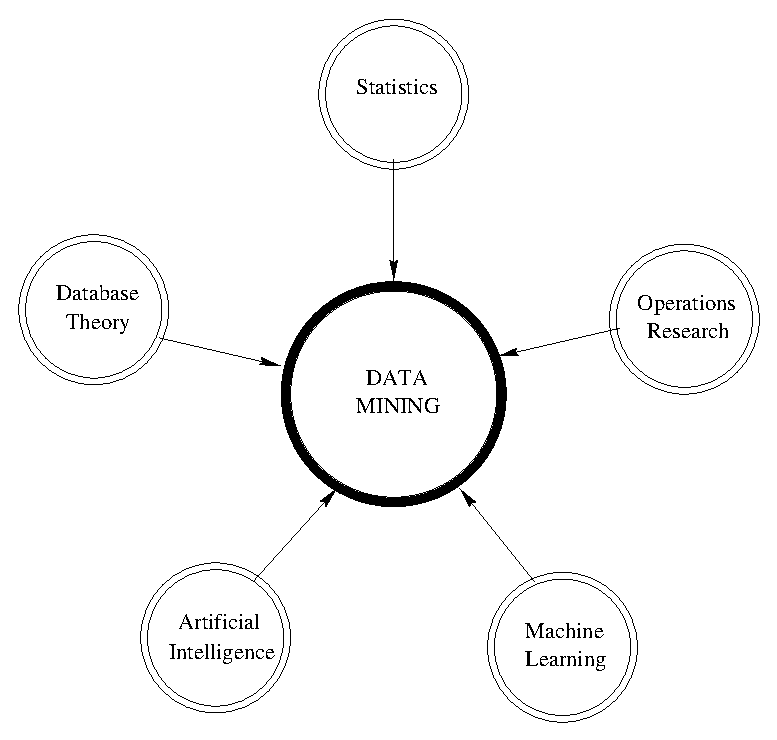
\includegraphics{figures/dm_process}}}
\caption{\label{fig:dm_process}Components of the Data
Mining Process}
\end{figure}
\index{Data Mining Components}  

\section{The Goal of the Thesis}\label{sec:int_hyp}
\index{Thesis Goal}

The ability to discover {\em knowledge} from a database which is not
explicitly represented in the data is clearly a desirable goal. We
propose that such {\em data mining} can be achieved using NDs,
generalisations of the FD, 
which themselves have a well-defined semantics for application within
the relational model. The application of NDs allow data
mining principles to be exercised on categorical data, often the bulk
of many corporate databases, or a combination of categorical and
numerical data. 

\smallskip
We show how relations containing indefinite or temporal data satisfy
numerous ND sets, being either definite instances of indefinite data
or possibly changing ND sets over time. The ND sets satisfied are
obtained from an initial template of FDs which is supplied by the
user; alternatively, it would be possible to mine for ND set
satisfaction. In the indefinite
domain the ND sets are satisfied in definite instances of the same indefinite
relation. We show how {\em resampling}, a computationally
intensive sampling procedure, may be applied on increasing sample
sizes to determine an approximate fixpoint upon which a heuristic based
hill-climbing algorithm is employed to find a suitable ND set
approximation to functional satisfaction. 
In the temporal domain the ND sets may change over time
for the same attributes; we
show how resampling and other time series statistics may be employed
to determine {\em properties} which may hold over time, using a logic
we have developed. Our data
mining framework thereby discovers information using many ND set
approximations upon which statistics are applied, varied for the
domain in question, to make further inferences from the data.

\section{Knowledge Discovery in Databases and this thesis}\label{sec:int_kdd}
			\index{Knowledge Discovery!Goals}
			\index{Knowledge Discovery!Outline}
			\index{Machine Learning!and Data Mining}
			\index{Pattern Discovery}
			\index{Data Warehouse}

 
\begin{figure}
\centerline{\scalebox{0.5}{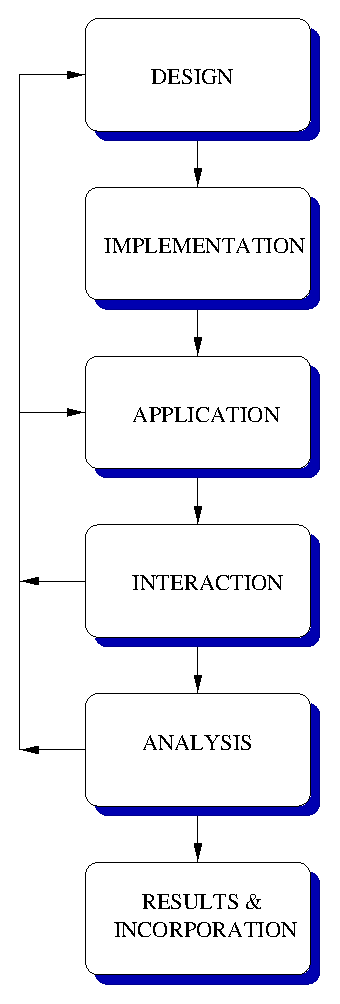
\includegraphics{../literature/kd_process.eps}}}
\caption{\label{fig:kd_process}The Knowledge Discovery
Application Cycle}
\end{figure}

The following widely accepted definition is due to \cite{kdd96}:

\begin{definition}[Knowledge Discovery in Databases]
\begin{rm} Knowledge Discovery in Databases is defined as {\em the
nontrivial extraction of valid, previously unknown, potentially
useful, and ultimately understandable information from a
database}. $\quad\Box$ 
\end{rm}
\end{definition}
\index{Knowledge Discovery!Outline}		

Knowledge Discovery may only provide {\em potentially} useful
information given that it may frequently discover relations, possibly
weak, between unconnected real-world information or even relations
that do not serve the interests of the user.  This includes the
possible discovery of redundant information. For instance, in a
medical database a system may discover a dependency $pregnant
\rightarrow female$ implying that all pregnant patients are female;
obviously such information is superfluous. Methods 
to prevent such redundant information generation may include the
specification of trivial associations before the mining process takes
place and continuous interaction with an expert, a much understated
component of knowledge discovery, defined as {\em data
archaeology} \cite{ba96}, as well as provision of a dependency
template upon which knowledge is discovered.   

\medskip
Knowledge discovery comprises a number of component parts including
data cleansing, design, warehousing and mining as well as expert
analysis, detailed in Figure~\ref{fig:kd_process}. Databases within
data warehouses are now frequently designed with a view to data mining
operations; where the goal of the database is {\em reliable storage}
the goal of the data warehouse is {\em decision support}
\cite{fay98b}. The process of data cleansing includes collecting data 
from different sources and processing it into a homogeneous form. The
design and implementation of a capable knowledge discovery tool will handle
these stages. Figure~\ref{fig:kd_process} displays a generic cycle
for knowledge discovery. It highlights the requirement that
interaction and analysis of the system may need to return to the
design stage if initial results suggest comparison with new data, which
may have been omitted, or the data cleansing stage has to be repeated
with new error parameters, perhaps to adjust the error and confidence
for noise within the database.  
Recent work has included
research on formalising the data warehouse \cite{hgmw95,inm96a} as
well as significant
data cleansing research.  Interesting as the issues of data
cleansing and warehousing are, we do not consider them further within
this thesis, concentrating on data mining.

\medskip

Knowledge
discovery refers to the process of extracting patterns and relationships 
from the data whereas data mining refers to the actual process of applying
these algorithms to the data, though many of the boundaries are vague.
In data mining applications a key requirement is 
the preparation of data for analysis. In Figure~\ref{fig:kd_process},
an example of a KDD application cycle, we assume that the
design and application components handle any required data
cleansing. Many data mining algorithms may also divide the data into
suitable training and validation subsets.   
Data Mining encompasses a number of different
approaches, such as clustering, data summarisation, learning
classification rules, finding dependency networks, 
and anomaly detection.  Data Mining is seen as a research frontier
for both database research and machine learning. Many other AI based techniques, such as Natural Language 
Processing and Distributed AI methods, are also increasingly included
\cite{kdd96}.  Machine Learning can be said to be the use of {\em
sophisticated} algorithms to generate and then process information,
for eventual understanding. \cite{xiao95} characterises learning from a
database as a triple $\langle$ D, C, A $\rangle$ where 
D is the data, C the {\em concept biases}, and A the language in which to
phrase the definitions. He also notes that as a database stores no  
negative information induction should be performed cautiously to avoid
over generalisation.
\medskip

Data Mining has been defined as the application of algorithms, within
the limits of computational efficiency, that produce a set of
expressions $E$ which represent patterns expressed in a well-defined
language over a data set $F$ \cite{kdd96}. There are a number of ways to
represent $E$, including: association rules \cite{ais93,toi96b}, rough
sets \cite{ziar91,incunc93}, temporal logic \cite{pt96,bt98}, and
FDs \cite{km95}. This 
latter class consists itself of many well-developed approximation
techniques including Fuzzy FDs \cite{bdp94}, PAC-approximation
\cite{at94,km95}, and probabilistic approximations
\cite{psm93,pk95,hkp98}. To this category we add NDs for pattern
expression \cite{cl98}. Their suitability to this task is shown via
their satisfaction of {\em lattice properties} from which measures for
approximation can be formed and the desirability of
mining NDs from databases. Mined NDs, expressed as {\em cardinality
constraints} (equivalent to NDs with empty left hand sides), have
recently been used to
reverse-engineer ER-models in \cite{sou98}. We also develop a
restricted temporal logic for discovery of patterns using NDs as our
atoms \cite{cl98f}.

\medskip

To date knowledge discovery research has focused on application
within relational databases containing definite information. However,
the advanced functionality of DBMSs extend the set of
data types beyond that of strict numerical or categorical data to
include NULL value representation \cite{lip79,il84}, the most common
interpretation being that a value
exists but we do not currently know what it is. The literature has
extended this to handle indefinite or disjunctive information where a
value might now be, for example, Tuesday or Wednesday, implying that
we know the value is one of a finite set \cite{inv91,vn95}.  To allow DBMSs to
handle scheduling 
and planning processing and querying directly the ability to store 
indefinite information is paramount. Data Mining techniques will then
have to be extended to encompass these data types. We show for the
case of NDs in \cite{cl98} how definite instances (or possible worlds)
of an indefinite relation satisfy different ND sets; other
FD approximation methodologies can be applied similarly.

\medskip
\index{Data Mining!Introduction}

Data Mining algorithms are bounded both by potentially huge data sets
and the limits of a computationally efficient methodology. Therefore,
sampling and the use of randomised algorithms for data mining have
been utilised \cite{km94,gms97,cl98b}. Sampling within data mining has
been well studied \cite{km94,jl96}; to this we include the use of
resampling for data mining. Resampling is a computationally intensive
sampling methodology for non-parametric data; the distribution is
unknown for most data sets. Its use allows for information about the
distribution of data to 
be made and has a wider range of application than standard
sampling. Many data mining algorithms seek to make inferences from
sample data; classical statistics refers to this as {\em estimation}. 
Our work incorporates resampling processes \cite{efro79,et86,et93}
to achieve this. Heuristics are often required for knowledge to be
discovered;
in such cases randomised algorithms may allow the efficient processing of
data for discovery. Indeed for a theory to be verified without error
the complete data set needs to be examined though only one violating occurrence
is required for falsification. Randomised algorithms and sampling allow for 
efficient analysis to be achieved utilising this fact. We use randomised
algorithms and resampling to find approximate solutions to the
{\em consistency problem}, known to be NP-complete, which is the problem of
searching for a possible world within an indefinite relation that
satisfies a given FD set \cite{vn95,cl98b,cl98}.

\medskip

Temporal
Databases have been a significant area of research in the last few
years \cite{tcg93,ct95}, unsurprising given the need for temporal
support in real-world applications, particularly in the financial and
medical domains. Building on this work is the rapid rise of, and need
for, temporal data mining applications.  
Much of Temporal Knowledge Discovery relates to forecasting events in the
future and analysing 
patterns which occur over time. Indeed, these goals are closely
related to time series analysis, a well established research field in
statistics and econometrics \cite{end95,naze88}. Nearly all databases
in use contain a 
temporal component and there has been much recent data  mining work on
temporal knowledge discovery \cite{alss95,pt96,bc96,bt98}. 

\medskip

Data mining and statistics have been substantially analysed
\cite{fhs96,gmp97}. One of the prime goals of data mining
is that of predicting values and this is inherently related to the
representation of temporal data and {\em time series analysis}. Time
series analysis when applied in a 
 database is used for anything from identifying demand and modifying
supply accordingly or for calculating patterns and changes in salary over time
to predicting the expense of projects within different time
periods. Until recently there was minimal use of time series analysis
techniques within temporal databases \cite{smd95}.

The Classic multiplicative model views time series as containing four
parts, namely trend, cycles, seasonal, and irregular patterns.
Trends may be up or down and can be used to characterise the time
series over a long time irrespective of short term fluctuations.
Cycles display a recurring up and down movement around trend levels,
including expansion and contraction. Seasonal patterns complete within
a given time period. Finally, irregular patterns account for erratic
changes in a time series and may be modelled as noise in the data.
\smallskip

The above may be understood using many techniques including trend
moving averages, ratio-to-moving averages (for deriving 
the seasonal component), and difference equations for model
representation. Using these time series may be extrapolated.
Related issues are (1) granularity changes (2) application of moving
windows, and (3) attribute value transformation. The temporal logic we
present, as well as the related work we survey
\cite{frm94,lai93,alss95,dgm97,dlm98}, is closely linked with many
aspects of (stationary) time series analysis. \cite{gmp97} also
tackles the issues of how data mining is extending and not simply
repeating previous statistical research. There have been significant
use of data mining algorithms incorporating statistical
functions, not least in the scientific domain in applications as
diverse as astronomical cataloguing through to geological sensing for
earthquake detection \cite{fhs96}.

\medskip

Recently there have been a number of different approaches to temporal
data mining, stemming from machine learning work on pattern
matching \cite{lai93,alss95}. There seems to be a demarcation between research based on
data mining from temporal databases and research using time series as
the input data set from which knowledge is to be discovered. Our
approach allows for discovery from either or a combination of the
two, given that in each case only series of
numbers change over time. 

\medskip

Temporal logic is used for temporal data mining in
\cite{pt96,bt98}. It has been shown to be sufficient for expressing
temporal relationships that have been discovered. If more complex
relationships are required, such as, say, correlation between two data
sets temporal logic does not have the functionality to express this
without an explicit {\em correlation function}. Therefore
we present a logic with statistical
functionality so that such values are embedded within the logic. Given
that the sentences of the logic express results of statistics
we do not have to present {\em confidence} and
{\em frequency} values (akin to work
on association rules \cite{ais93,kmrtv94,hkmt95}) for the rules that
we discover as our rule discovery 
itself is representative of specific statistical values. Our work on
temporal relations is pattern focused; we do 
not attempt to discover a global model, the undoing of many time
series analysis studies, but logical rules which describe local behaviour
on subsequences of the temporal data set. Of course these can be, if
desired, extended to global conditions.
It is interesting to note that discovery in this
sense is closely linked to the power of the query language. Similarly,
we may view rule discovery using temporal logic as directly dependent on
the expressiveness of the logic.
Patterns within a (temporal) database may be referred to as {\em properties}
which model the data. Temporal logic for property satisfaction is a
well-researched area within program verification. Properties used to
express the correctness of a temporal system also have application
in data mining where a database with many states may be viewed as a
temporal system. We claim that these properties are therefore suitable
as {\em candidate patterns} for potentially interesting knowledge
discovery. 

\medskip

The real-world desire for ever more information and knowledge
precludes data mining from being anything but a significant research
area. Many different mechanisms for expressing patterns have been
developed and we believe that NDs, though not a panacea for expression
within data mining, are widely applicable and easily understood. 
To illustrate, an ND $STUDENT \to^5 COURSE$ in a timetable relation
specifies that a student can take at most 5 different courses; it is
clear that such data may often need to be represented and in current
DBMSs this data would satisfy no built-in constraints.
The progression towards a standardised query language for data mining
\cite{cha98} 
would benefit from their inclusion as we note their utility in
different domains.

\section{Main Results and Contribution}\label{sec:int_contrib}
\index{Thesis Contribution}

We provide a novel approach to data mining. We show how, in databases
containing indefinite and temporal information, given an FD set F we
form sets of approximations to F which may be satisfied for
different definite instances of the indefinite relation or over time
in a temporal relation. We choose to express these approximations as
sets of NDs;
other expressions may also be appropriate, such as a probabilistic
approximation \cite{psm93}. In either indefinite or temporal databases
we can use these sets to obtain statistics to determine how they
may change in the indefinite relation or over time. We show
how resampling can be applied to these sets to make inferences from
the data. For indefinite relations we present a dynamic resampling
process which allows for resampling on increasingly large sample sizes
until an approximate fixpoint is reached. This provides an upper bound
on sample size which is then used in a heuristic based hill-climbing
algorithm. 
For temporal relation
sequences we may take moving averages or create resampled sequences to
determine how patterns, expressed in the form of {\em properties}, are
satisfied at various time points. 

\medskip

We now outline our methodology as a general framework. We
take a large set $\alpha$ of approximations to a given FD set and then
apply resampling to 
$\alpha$ to draw conclusions on the nature of the data in the
database. The exact method of the application of resampling, and the
use of other statistical functions, differs with the type of data we
are mining. This framework is applicable to other domains, extending
the traditional mining approaches of simply using approximations to
dependencies to infer information. Indeed, we assume that an FD set is
provided by the user as a template in both indefinite and temporal
domains; this FD set may be modified by a system user to compare
results for different dependency sets. We shall demonstrate how it is
possible to utilise temporal and indefinite domains from which the
approximations, in our 
case NDs, are taken to make further discoveries from the relation
which is being mined. 

\smallskip
\noindent This thesis makes the following specific contributions:
\begin{enumerate}
\item NDs are shown to be effective and useful for 
data mining in that they provide a clear notion of proximity to FDs.
NDs are shown to be able to efficiently and accurately approximate FDs
in a relation with an easily understood semantics. 
An evolutionary database design procedure is introduced as a 
motivation for real-world ND applications as a precursor to their application
in non-standard database domains. The lattice properties of NDs are
exploited to provide a metric for data mining which we use in this work. 
\item We provide a detailed study on an approach which uses NDs to
provide approximations to the Consistency Problem, namely the
NP-Complete problem of finding a definite world that satisfies a set
of FDs within a relation containing indefinite data. 
\item Procedures for applying the Bootstrap, a resampling methodology \cite{et93}, within relations containing
indefinite and temporal data are defined and shown to be useful via extensive
simulations. They include a dynamic procedure for application of the
bootstrap in indefinite relations for sample size determination. 
\item A temporal logic for NDs is presented. This logic is then used
for mining sequences of relations. We examine the sequences for proximity
to FD set satisfaction, expressed as NDs, and compare this
to standard time series 
analysis. The logic is transferable to standard time series and other
linearly ordered numerical data sequences.
\item We present a model for the application of our temporal data
mining system to a sequence of temporal relations. Results using
financial time series of stock prices from the oil,
finance and retail sectors are presented and analysed.
\end{enumerate}

The thesis also presents a taxonomy of standard and temporal 
dependency data mining, placing our work in context, as well as making
suggestions for future research. 

\section{Outline of the Thesis}\label{sec:int_outline}
\index{Thesis Outline}

After this introduction, Chapter~\ref{chap:review} formally introduces
the required relational database theory so that the remainder of the
work is self-contained.  All of the relevant theory presented is
placed in the context of this research and related work. Additionally,
we survey related data mining research, focusing on three areas:
\begin{enumerate}
\item
We examine functional dependency data mining and the methods used to
find approximations to FDs \cite{km95,at94,Mann92,sf93,HS95,pk95,bel95b,psm93}, of which using NDs is part of our
contribution, shown in Chapter~\ref{chap:numdep}.
\item We briefly
examine work conducted on 
indefinite information, related to our study of the consistency
problem.
\item Temporal data mining research is discussed so that
the reader is able to appreciate the contribution of the
work in Chapters~\ref{chap:templog}
and~\ref{chap:tempresult}. 
\end{enumerate}
Chapter~\ref{chap:review} concludes with a
brief presentation of
resampling in statistical applications, which is then expanded upon in
Chapters~\ref{chap:consistency} and~\ref{chap:tempresult}.

\medskip

Chapter~\ref{chap:numdep} presents ND theory with regard to data
mining, including a {\em chase procedure} for NDs. The chase
procedure may be used to modify a relation to satisfy a given ND set
allowing us 
to test whether or not an ND set implies a specific ND.
We show how a
data mining distance function is used for assessment, related
to approximation work presented in
Chapter~\ref{chap:review}. Additionally, research on applying NDs for
mining within relations is discussed and compared with other
approaches. We also present a practical database design tool for randomly
evolving example relations which satisfy FD sets.

\medskip
Chapter~\ref{chap:consistency} then introduces
the consistency problem and its applications. We present randomised
algorithms which use NDs and the chase procedure for indefinite
relations together with a novel application of resampling to determine
sample size. Results of extensive simulations applied to
randomly generated indefinite relations are examined. We
also discuss the 
usefulness of the chase procedure as a heuristic.

\medskip

Chapter~\ref{chap:templog} moves on to temporal data mining. We
motivate the need for rules in temporal data mining, introduce our
logic for temporal data mining, examine the logic and introduce the
notion of temporal properties which we use in our temporal data mining
environment. This logic is then assessed against a standard time series
analysis which could be conducted on any time series data set and also
on any temporal sequence of relations satisfying ND sets in each
state over fixed intervals. Chapter~\ref{chap:tempresult} presents the
details of our temporal 
rule discovery system, the use of resampling, and results from data
sets studied, concluding with a discussion of future work together
with an analysis of the utility of our temporal data mining approach.

\medskip

Finally in Chapter~\ref{chap:conclusion} we give our concluding
remarks and present a final discussion of the work, introducing
avenues for further research and stating the open problems that remain.


\section{Notation}\label{sec:not}
\index{Notation}

We presented an index of the symbols used at the beginning of the thesis
in the symbol index.

\smallskip

This thesis adheres to the standard notational convention generally followed in
relational and deductive database texts, notably \cite{Ullm88}.  R
refers to a relation 
schema, denoting a finite set of attributes,  and $r$ to a relation over R,
denoting a finite set of tuples.  Uppercase letters (possibly
subscripted) refer to attributes if they are from the beginning of the
alphabet such as A, B, C and to attribute sets if they are from the
end of the alphabet such as X, Y, Z.  Tuples are referred to by
lowercase $t$ and $u$ (possibly subscripted).

\medskip

Lowercase letters (possibly subscripted) refer to constants if they
are from the beginning of the alphabet such as $a$, $b$, $c$ and to
variables if they are from the end of the alphabet such as
$x$,$y$,$z$.  Predicate symbols (possibly subscripted) of arity $\ge
0$ are referred to by $p$, $q$ and $r$. 
We use $\mid X \mid$ to refer to the cardinality of set $X$ and simply
$X$ to denote the singleton set $\{ X \}$. The nonempty powerset of a
set $X$ is denoted by $\cal P$($X$). From the 
relational database literature, we refer to the union of
two sets $X \cup Y$ by $XY$. The end of a definition or proof is
denoted by $\Box$.



\chapter{Relational Database, Data Mining, and Statistical
Theory}\label{chap:review}

The aims of this chapter are to provide the requisite
background to be able to read the thesis as a self-contained body of
work as well as enabling the reader to appreciate this research within
the wider fields of both relational database theory and data mining.

In Section~\ref{sec:db_for_dm} we present the relationship of this
work to both database and data mining theory. 
In Section~\ref{sec:relmod} we introduce the relational database theoretic
concepts relevant to this thesis and in Section~\ref{sec:datmin}
we introduce the area of data mining, concentrating firstly on dependency data
mining so that the reader can fully appreciate the context of
Chapter~\ref{chap:numdep} and then temporal data mining for the
background of Chapters~\ref{chap:templog}
and~\ref{chap:tempresult}. In later chapters we will refer to 
the definitions presented in~\ref{sec:relmod} and~\ref{sec:datmin}
as and when they are initially used.

\section{Database Theory for Data Mining}\label{sec:db_for_dm}
\index{Data Mining!and Database Theory}
There has been significant work in the data mining community on the
mining of {\em data dependencies}, both in standard \cite{psm93,km95} and
temporal environments \cite{bwj96}. Much of this concentrates solely
on the discovery process, in effect working totally within a machine
learning (ML) context, i.e. \cite{she91}; scant regard is paid to the
database theory upon which the dependencies are based. Though we
do not question the quality of this work because of this omission we
believe that NDs which fit into the
relational model, both for design and, as we show in this thesis, data
mining, are a valuable tool. Until recently, much data mining research
was disjoint from database 
theory, based within statistics or machine learning though there is
now a body of work on unifying these areas \cite{cha98}; this thesis
requires an appreciation of both.
We introduce the background material on
database theory in Section~\ref{sec:relmod} to clarify
later work on Armstrong relations and the chase procedure, a
theorem proving tool for FDs in a relation, as well as our use of indefinite
information for the consistency problem. Theoretical work on FD
behaviour has directly led to the 
creation of numerous data mining methodologies which we introduce
in~\ref{subsec:fdmining}.  Section~\ref{sec:relmod} concludes with a
presentation of 
temporal databases and dependencies.

Section~\ref{sec:datmin} introduces aspects of dependency data mining,
including a discussion of the relationship to NDs. We provide a
discussion of measures based 
on aspects of FD theory in~\ref{subsec:fdmining}. We then introduce
temporal databases and dependencies before moving on to temporal data
mining and rule discovery from time series, closely
related to work in Chapters~\ref{chap:templog} and~\ref{chap:tempresult}.
This section concludes with a brief overview of sampling in data
mining followed by an informal introduction to resampling, useful for
later work presented on indefinite and temporal relations.

\section{Relational Database Theory}\label{sec:relmod}
\index{Relational Database|see{Relational Data Model}}

We now present the relational database theory required within this
thesis. The reader is referred to
\cite{databasefound,atze93,Maier83,Ullm88} for a complete coverage of
the area.

\subsection{The Relational Model}
\index{Relational Data Model}

In 1970, E. F. Codd introduced the relational model \cite{cod70}, with
relations as the data structure,  so
that database users need not concern themselves with the physical
storage of data.  This allowed independence between programs and their
machine representations by providing a sound basis for describing the
structure of data and operations for data manipulation without the
need for consideration of the internal machine
representation. Subsequently other data models have been developed,
including the Entity-Relationship model, for high level conceptual
database modelling, and object-oriented data models
\cite{kim90,databasefound}. The latter were primarily developed to
combat the growing requirements for complex data manipulation; we do
not make further reference to these data models and remain within the
confines of the relational model in this thesis. Its universality and
ease of data 
manipulation does not require further justification. We now formalise the
relational model.

\index{Universe}
\begin{definition}[Universe]
\begin{rm}
A universe $\cal U$ is a finite, fixed set of symbols that represent the 
column names which can appear within a relation.  They are referred to
as attributes. $\quad\Box$
\end{rm} 
\end{definition}

\index{Attribute Domain}
\begin{definition}[Attribute Domain]
\begin{rm}
The domain of an attribute A $\in \cal U$, denoted by DOM(A), is the
countable set
of possible values which can be members of A.  This is the set
of values which can appear in a column of A.$\quad\Box$
\end{rm}
\end{definition}
\index{Relation Schema}
\index{Relation}
\begin{definition}[Relation Schema and Relation]
\begin{rm}
A relation schema R is a subset of the universe $\cal U$.  The elements
of a relation schema are denoted by $\{$ A$_1$, $\ldots$, A$_n$ $\}$.
A {\em tuple} over R is an element of DOM(A$_1$) $\times \ldots \times$
DOM(A$_n$), where $\times$ refers to the cartesian product.  An instance
of a relation over R is a finite set of tuples defined over R. $\quad\Box$
\end{rm}
\end{definition}

A relation consists of a finite set of tuples where each tuple
represents an entity.  A relation is therefore simply an entity set. 
Each tuple can be considered a row if we assume
the table representation of a relational database.
\index{Database Schema}
\begin{definition}[Database Schema and Database]
\begin{rm}
A Database Schema over $R$ is a finite set of relation schema $\{$ R$_1$,
$\ldots$, R$_n$ $\}$.  A database over $R$ is a finite set $d$ = $\{ r_1,
\ldots, r_n \}$ such that each $r_i \in d$ is a relation over R$_i \in
R$. $\quad\Box$
\end{rm}
\end{definition}

The relational algebra is presented by Codd \cite{cod70} in the context of
deriving desired result relations from other relations.  The operations include
{\em selection}, {\em projection}, defined below, {\em join}, {\em
union}, {\em difference}, and
{\em renaming};  all are defined in
\cite{databasefound,atze93,Date95,Maier83,Ullm88}.
\index{Projection}
\begin{definition}[Projection]
\begin{rm}
The projection of an R-tuple $t$ onto a set of attributes Y $\subseteq$
R, denoted by $t[$Y$]$ (also called the Y-value of $t$), is the
restriction of $t$ to the attributes in Y.  The projection of a
relation $r$ onto Y, denoted as $\pi_{\rm Y}$($r$),
is defined by $\pi_{\rm Y}$($r$) = \{ t[Y] $\mid$ t $\in$ $r$ \}.$\quad\Box$
\end{rm}
\end{definition}

We now move on to the representation of constraints in the relational
model required to ensure the maintenance of integrity within a
database. Data mining now often uses such constraints and constraint
approximations to discover previously unknown and non-trivial
information \cite{kdd96}.


\subsection{Functional Dependencies}
\index{Integrity Constraints}
			\index{Data Dependencies}
			\index{Functional Dependency}
			\index{Determination}
			\index{Key}
			\index{Functional Independency}
			\index{Axiomatisation}
		 	\index{Soundness}
			\index{Completeness}
Integrity constraints, or data dependencies, allow a database to have
associated with it an intended meaning or semantics for the tuples
within the database.  The most common
constraint is the FD introduced in
\cite{cod72}, its prevailing application in practice is as
a key dependency.  FDs were given a {\em sound} and
{\em complete} axiomatisation in \cite{Arms74}.  We note that {\em
soundness} implies that each dependency, which is derived using a
finite number of applications of an axiomatisation from a given set,
holds. {\em Completeness} implies that valid each dependency which holds can be
derived using the axiomatisation. FDs
are restricted first order logic (FOL) sentences shown in
\cite{sdpf81} to be equivalent to Horn clause statements, relating
determinations to logical implication \cite{fag77,logicfound,mak87}. 
There has been extensive work on the theory of FDs,
of which some seminal contributions are
\cite{Arms74,fag77,bb79,sdpf81}. Although work on FD theory has somewhat
exhausted itself there has recently been extensive work in data mining for
approximating FDs \cite{Mann92,sf93,bb95,hkp98}.

\begin{definition}[Data Dependency]
\begin{rm}
A data dependency is a restricted integrity constraint incorporating a
(specified) property that is to be satisfied by all instances of the database
schema. $\quad\Box$
\end{rm}
\end{definition}

Dependencies within the relational model allow for the incorporation of a more
complex semantics via meta-data representations. We now formalise the
FD, its axiom system, and the closure of FD attribute sets. 

\index{Functional Dependency}
\begin{definition}[Functional Dependency (FD)]
\begin{rm}
A {\em functional dependency} over R (or simply an FD)
is a statement of the form X $\to$ Y, where X, Y $\subseteq$ R. $\quad\Box$
\end{rm}
\end{definition}
\medskip
 
 F {\em is known as a set of FDs over} R and X $\to$ Y 
{\em is  a single FD over} R. We denote logical implication by $\models$.
A key dependency is an FD of the form X $\to$ R for some X $\subseteq$
R. 
\index{Functional Dependency!Satisfaction}
\begin{definition}[Satisfaction of an FD]\label{def:sat}
\begin{rm}
Given $r$,  a definite relation over R,
an FD X $\to$ Y is {\em satisfied} in $r$,
denoted by $r \models$ X $\to$ Y, whenever
$\forall t_1, t_2 \in$ $r$, if $t_1$[X] = $t_2$[X] then $t_1$[Y] = $t_2$[Y].
A set of FDs F is {\em satisfied} in $r$,
denoted by $r \models$ F, whenever
$\forall$ X $\to$ Y $\in$ F, $r \models$ X $\to$ Y.$\quad\Box$
\end{rm}
\end{definition}
\medskip
\index{Armstrong's axioms!for FDs}
FDs obey a set of axioms, shown to be sound and complete in
\cite{Arms74}, which are:
\begin{definition}[Armstrong's Axioms for functional dependencies]
\begin{rm}
Given a relation schema R and X,Y,Z $\subseteq$ R:
{\line
\begin{description}
\item[Reflexivity] If Y $\subseteq$ X, then X $\to$ Y
\item[Augmentation] If X $\to$ Y then XZ $\to$ YZ
\item[Transitivity] If X $\to$ Y and Y $\to$ Z, then X $\to$ Z$\quad\Box$
\end{description}
}
\end{rm}
\end{definition}


\index{Closure!of an attribute set}

\begin{definition}[Closure of an attribute set]
\begin{rm}
Given a set F of FDs over a set of attributes X in schema R the closure of X
under F, denoted X$^+$, is the set $\{$ A $\in$ R $\mid$ F $\models$ X
$\to$ A $\}$. $\quad\Box$
\end{rm}
\end{definition}

X$_{\rm F}^+$ refers to the closure of X with respect to F, that is
the set of all attributes A $\in$ R such that X $\to$ A holds in F.
We define F$^\star$ to be the closure of F such that trivial
FDs of the form X $\to$ Y, where Y $\subseteq$ X, are excluded.

\begin{definition}[Non-trivial closure]
\begin{rm}
F$^\star$ = $\{$ X $\to$ Y $\mid$ XY $\subseteq$ R and Y $\subseteq$
X$_{\rm F}^+$ $-$  X $\}$. $\quad\Box$
\end{rm}
\end{definition}

\begin{definition}[Closure of a set of attribute sets]
\begin{rm}
Given an FD set F we denote the closure of all possible
attribute sets under F by CL(F). This is defined as
CL(F) = $\{$ X $\mid$ X $\subseteq$ R and X$_{\rm F}^+$ = X $\}$. $\quad\Box$
\end{rm}
\end{definition}

Note that the schema R is always included in the closure of attribute
sets for any FD set. The next lemma shows that F$^\star$ and 
CL(F) are equivalent in characterising a set of FDs F. The
non-trivial closure is relevant in data mining measures,
discussed in Section~\ref{subsec:fdmining}.

\begin{lemma}
\begin{rm}
Given two sets of FDs, F and G, we then prove 
G$^\star$ $\subseteq$ F$^\star \equiv$ CL(G) $\supseteq$ CL(F)
\end{rm}
\end{lemma}

{\em Proof. (if) }
Assume, to the contrary, that CL(G) $\not\supseteq$ CL(F).
Therefore $\exists$ X $\in$ CL(F) such that X $\not\in$ CL(G), implying
that X is not closed in G. 
Then X$_{\rm G}^+$ = XY, for some attribute set Y.
 This implies that X $\to$ Y is in G but
not in F, yet G$^\star \subseteq$ F$^\star$, leading to a
contradiction.

\smallskip
{\em (only-if)}
Assume, to the contrary, that G$^\star \not\subseteq$ F$^\star$. 
Then $\exists$ X $\to$ Y $\in$ G$^\star$ such that X $\to$ Y $\not\in$
F$^\star$. 
Then Y $\subseteq$ X$_{\rm G}^+$ but Y $\not\subseteq$ X$_{\rm F}^+$, 
and so X$^+_{\rm G} \not=$ X$^+_{\rm F}$.
Given that CL(G) $\supseteq$ CL(F) it must be the case that 
any closed set in F
must be closed in G, and so we have a contradiction. $\Box$

\medskip
\index{Closure!of a set of FDs}
\begin{definition}[Closure of a set of FDs]
\begin{rm}
Given an FD set F we denote the closure of F by F$^+$. 
This is defined as
\begin{displaymath}
\mbox{F}^+ = \{\mbox{X} \to \mbox{Y} \mid \mbox{XY} \subseteq \mbox{R}
\mbox{ and } \mbox{F} \models \mbox{X}
\to \mbox{Y}  \}\quad\quad\Box
\end{displaymath}
\end{rm}
\end{definition}


An algorithm to compute the closure of a set of FDs is in 
\cite{databasefound,atze93} which runs in time linear to the size of
the set FDs. The
concept of a maximal set is now introduced; its data mining
applications will be briefly discussed in
Section~\ref{subsec:fdmining} and Chapter~\ref{chap:numdep}.
\index{Maximal Set}
\begin{definition}[Maximal Set]
\begin{rm}
Given X, a subset of schema R, and A $\in$ X then
a set Y $\subseteq$ X is a {\em maximal} set for A, if F
$\not\models$ Y $\to$ A and for any
Z $\subseteq$ X such that Y $\subset$ Z we have F $\models$ Z $\to$
A.$\quad\Box$ 
\end{rm}
\end{definition}

\begin{definition}[The set of all maximal sets]
\begin{rm}
$max$(F,X,A) = $\{$ Y $\subseteq$ X $\mid$ Y is a maximal set such that
F $\not\models$ Y $\to$ A $\}$.  If F is understood from the context then it
is written simply $max$(X,A); $max$(X) denotes the union of $max$(X,A)
where A $\in$ X.$\quad\Box$
\end{rm}
\end{definition}


A maximal set is an attribute set X which for some attribute A is
a largest possible set {\em not} determining A. We also define
generator sets. The generator function, GEN, omits those sets from the
closure of an attribute set which can be formed by the intersection of
other sets in the closure to obtain a more concise
representation. Theorem 13.1 of \cite{Mann92} shows that $max$(X) = GEN(X).
\index{Generator Function!and Maximal Sets}
\begin{definition}[The generator function]\label{def:GEN}
\begin{rm}
The generator function produces a set for X such that
GEN(X) = $\{$ Y $\in$ CL(X) $\mid$ Y $\subset \bigcap \{$ W $\in$
CL(X) $\mid$ Y $\subset$ W $\}\}$$\quad\Box$
\end{rm}
\end{definition}

We now define the cover of a set of dependencies, useful for
discovering equivalent FD sets.

\index{Cover!of a dependency set}

\begin{definition}[Cover of a set of Dependencies]
\begin{rm}
Given sets F and G of FDs, F is a {\em cover} of G
if F$^+$ = G$^+$. A {\em cover} G is minimal for F if there does not
exist a cover H of F such that $\mid$ H $\mid$ $<$ $\mid$ G $\mid$. A
minimal cover is necessarily nonredundant,  
that is, $\forall d \in$ G we have  G $\backslash \{ d \} \not\models
d$, though nonredundancy does not imply minimality. $\quad\Box$
\end{rm}
\end{definition}

\begin{example}
\begin{rm}
From \cite{mr92}, the set F = $\{$ A $\to$ BC, B $\to$ AD, CD $\to$ E,
E $\to$ CD $\}$ and the set  G = $\{$ A $\to$ BE, B $\to$ A, CD $\to$
E, E $\to$ CD $\}$ are equivalent. This is proven by showing that G
$\models$ F and F $\models$ G.  The non-trivial 
cases are showing that F $\models$ A $\to$ E and G $\models$ $\{$ A
$\to$ C, B $\to$ D $\}$. To illustrate, A $\to$ C may be shown to hold
from G as we know A $\to$ E holds, by transitivity A $\to$ CD
holds, and therefore A $\to$ C is known to be satisfied by G. 
\end{rm}
\end{example}

To test if two covers, F and G, are equivalent we can check that
every X $\to$ Y $\in$ F is satisfied in G and vice versa.  Using the
algorithm presented in \cite{mr92} this can be done in time $O( \mid$ F
$\mid \|$ G $\| + \mid$ G $\mid \|$ F $\|)$, where $\|$ X $\|$ denotes
the number of attributes in X including repetitions. Alternatively, we
can check for 
equivalence of the maximal sets. We now introduce some notation to aid
the reading of the next section.
\index{Agreement set}
\begin{definition}[Agreement set of two tuples]
\begin{rm}
Given a relation $r$ over R, where $t_1$,$t_2$ are
two tuples in $r$ the agreement set is defined as
$ag(t_1, t_2)$ $=$ $\{$ B $\in$ R $\mid$ $t_1[$B$]$ $=$
$t_2[$B$]$$\}$. \newline 
The disagreement set is defined dually, disag($t_1$,$t_2$) = R
$\backslash ag(t_1, t_2) $.$\quad\Box$
\end{rm}
\end{definition}

Given an attribute A in disag(a,b) let X be the disagreement set of all
attributes for tuples a and b apart from A, i.e. X = disag(a,b) $\backslash \{$A$\}$.  
Then any set in the left-hand side of A must contain at least one
attribute of X. Why is this so?  Let us assume that it does not hold and
that for a member of the left-hand side of A an attribute of X is not
contained.  This implies, however, that there exist two tuples which disagree
on A when they have the same left-hand side.  Obviously this violates F and so is
not the case. X is therefore said to be a necessary set for A, used in
dependency mining \cite{Mann92}.

\begin{definition}[Agreement set of a relation]
\begin{rm}
Given a relation $r$ over attribute set R, the agreement set is defined as
$agr(r) = \{ ag(t_1,t_2) \mid$ $t_1,t_2 \in r \}$.$\quad\Box$
\end{rm}
\end{definition}


We now define Armstrong Relations (AR) and
follow this with a discussion of database design and its relationship
to data mining.

\subsection{Armstrong Relations}\index{Armstrong Relations}


\cite{Arms74} introduced the concept of an {\em Armstrong relation}:  

\begin{definition}[Armstrong Relation]\label{def:AR}
\begin{rm}
An Armstrong relation for F is a relation $r$ which satisfies F$^+$
and is such
that for every FD $\sigma \not\in {\rm F}^+$ for which  F$^+ \not\models
\sigma$, then $r$ violates $\sigma$.$\quad\Box$
\end{rm}
\end{definition}

In theory, Armstrong relations \cite{fag82,bdfs84,dt95,gl90,lev95,mr86}
serve as ``ideal'' example relations, since they satisfy exactly the set of
all logical consequences of the set of FDs specified, say F.
Thus an Armstrong relation provides an example for all FDs
that are logically implied by F and a counterexample for all 
those FDs that are not logically implied by F.
One of the problems with Armstrong relations is that, in general,
their cardinality is exponential in the size of F and the set of attributes, R,
over which F is defined \cite{bdfs84}. An Armstrong relation for a
set of FDs, if
deterministically generated \cite{Mann92}, always provides
the same resulting relation. It would be highly desirable if varying Armstrong relations
of different domain and tuple sizes may be generated as a side effect of 
the forming of example relations.

\medskip

\cite{fag82} presents a survey of Armstrong Databases  including
descriptions of the techniques for generating Armstrong Relations from
a set of FDs.  
These are: (1) Use {\em disjoint union } to create an isomorphic copy of each
relation and then form the union of all of the tuples in all of the
relations. For each FD $\sigma$ which is not a logical consequence of
the relations create a relation $r_\sigma$ which obeys F but not
$\sigma$. Then form the union for all {\em standard} FDs, where the
left hand side is non-empty, to give an
AR.  (2) Create {\em agreement
sets}. The agreement set is formed such that
GEN(F) $\subseteq agr(r) \subseteq$ CL(F). \cite{bdfs84} construct
an Armstrong relation by firstly computing the closure of the FD set
F, CL(F), and then constructing a relation such that $agr(r)$ =
CL(F). (3) {\em Direct
products }(used by \cite{gm85a} to prove no Horn clause
representation exists for NDs). A relation is created for each $\sigma$ outside
of CL(F) which violates $\sigma$ and satisfies CL(F). The direct
product of these is then formed. (4) Use the {\em chase procedure},
presented in Section~\ref{subsec:rev_chase}. Given
an Armstrong relation which obeys an FD set
F and violates all FDs outside of CL(F) form a model where all
FDs are violated using the chase which can cause new tuples and/or
constants to be added to the database. We shall see in
Chapter~\ref{chap:numdep} how an evolutionary technique using mutation
and guided by ND
satisfaction may often generate Armstrong relations \cite{cl96,cl98c}.

\medskip

\cite{fv83} shows that an Armstrong database may be generated for a
set of inclusion  
dependencies and standard FDs.  An inclusion dependency
states that if some combination of values occurs in one part of a
database it  must also occur in another part.  
\medskip

Lemma 3.1 \cite{bdfs84} shows that if $\Sigma$ is a set of FDs and $\sigma$ a
single FD such that $\Sigma \not\models \sigma$ then there exists a two tuple
relation that obeys $\Sigma$ but not $\sigma$.  A by-product of this result is
that it is always possible to add a tuple to a relation $r$ satisfying
$\Sigma$ which
violates $\sigma$.  A deficiency of deterministic processes for AR
generation are that
only one specific Armstrong relation is ever returned for a given FD
set. \cite{bdfs84} present an analysis on the upper and lower bounds of the
size of an Armstrong Relation based on the number of distinct entries 
in the relation, referred to as the generator sets which \cite{mr86} 
later refine. 
\cite{mr86} show that the size of a minimal Armstrong relation for a
normalised  scheme R depends strongly on the number of keys for R.
The possible exponential size of a minimal Armstrong relation depends
only on the number of dependencies, and not on the number of attributes. 

An Armstrong relation should be as small as possible, as should the
set of values used, though the smaller the relation the more difficult
it becomes for the designer to locate all of the anomalies as opposed
to an Armstrong relation which lists all examples of dependency
violations in a pairwise format.\\ 

\subsection{Relational Database Design}\label{subsec:reldbdes}
\index{Relational Database Design}
\index{Database Design|see {Relational Database Design}}
\index{Referential Integrity}
\index{Normalisation}
			\index{Redundancy}
			\index{Normal Form}
			
We now mention relational
database design related to work presented in
Chapter~\ref{chap:numdep}. Informally, database design attempts to
remove redundancy and facilitate querying by the use of normalisation.
A relation can be 
constructed to adhere to a series of increasingly restrictive normal forms introduced so as to prevent redundancy and (update) anomalies within the
database, discussed in
\cite{cod72,databasefound,atze93,Date95,Maier83,Ullm88}.  

\medskip

Keys provide the only method for tuple identification  in the standard
relational model, and they are
therefore central to the retrieval of information and good database design. There are many key
related properties whose determination is computationally intractable
\cite{lo78}. We now present the superkey class, used within Boyce-Codd
Normal Form.

\index{SuperKey}
\index{BCNF|see{Boyce Codd Normal Form}}
\index{Boyce Codd Normal Form}
\begin{definition}[SuperKey]
\begin{rm}
Given a relation scheme R and a set  $\Sigma$ of FDs which apply to
it, a  set of attributes X is a superkey for R if the FD X $\to$ R
$\in \Sigma^+$. $\quad\Box$ 
\end{rm}
\end{definition}

\begin{definition}[Boyce Codd Normal Form]\label{def:bcnf}
\begin{rm}
Given a relation scheme R and a set of FDs $\Sigma$ which apply to it,
R is in Boyce Codd Normal Form (BCNF) if for every non-trivial FD X
$\to$ A $\in \Sigma^+$, X is a superkey.$\quad\Box$ 
\end{rm}
\end{definition}


We assume that all relations discussed in this thesis
satisfy first normal form (1NF), where each relation is flat, and
present a database or relation satisfying BCNF as the ideal normal form,
where each non-trivial FD has a superkey as its left hand side. BCNF
attempts to 
overcome the deficiencies in 3NF by dropping the constraint that {\em
non-prime} attributes, those not in any key, which are allowed on the
right hand side of FDs may violate the normal
form . \cite{bb79}
present an analysis method to achieve a BCNF relation by splitting
relations successively which violate BCNF. No such procedures exist
which 
are guaranteed to be constraint preserving.  A non-mathematical
treatment of normal 
forms is given in \cite{ken83} which are then extended for temporal 
relations in \cite{jss92}. 
\medskip
\index{Example Relation}

\cite{sm81} introduced the
idea of example relations generated from a set of FDs and MVDs  for 
database design purposes. Example relations give the database designer 
a guide to the information within a relation associated with a given
set of dependencies. 
\cite{sm81} formalise a design technique which attempts to provide the
database designer an iterative method of obtaining the FD set which
most {\em characterises} a relation.  More recently  \cite{mr86,mr92},
approached various database 
design problems with the goal of formalising methods and tools to
produce schemas with specific properties. They 
introduce the technique of using example relations within the design
process, notably as ``an application of ARs'', by presenting an
algorithm to deterministically generate ARs for the benefit of the
database designer.  \cite{bdfs84} note how an
Armstrong relation, perhaps generated automatically from a set of FDs, is of
much use in the design process from an application point of view.
Automated database design has 
been seen as a goal for dependency theory \cite{bv84}.

\medskip

In \cite{cl98c}, summarised in Chapter~\ref{chap:numdep}, we present
 a probabilistic extension of this work, 
 allowing the database designer to view many different example
 relations, though not necessarily ARs, for any given FD set specified
 over R. The size of the relation is governed by the database designer.
 \cite{mr86} state,  ``A good example
 relation should not leave the designer any illusions about what can
 be stored in the database.'' Our algorithm for generating example
 relations achieves this. It is based on the following loop
which we envisage during the database design process:
\begin{enumerate}
\item The database designer specifies a set of FDs, F, 
 the maximum number of tuples in the example relation, $m$, and
the maximum domain size, $d$, for a relation. (The designer
has the options of specifying $m$ and $d$ so that relations
of different structure can be viewed.)
\item A random example relation satisfying F, 
having at most $m$ tuples, and a domain ranging
from 2 to $d$ values is generated. The quality,
in terms of its proximity to that of an Armstrong relation, for the 
FD set is measured and returned to the designer.
\item The database designer either accepts F or modifies the parameters
F, $m$ and $d$, 
and then returns to step (2).
\end{enumerate}

Two aspects of this work are discussed subsequently; the
evolutionary hill climbing algorithm which uses NDs in a hill climbing
fashion to obtain a relation satisfying an FD set is presented in
Chapter~\ref{chap:numdep} and the {\em
quality} function used to obtain a proximity to an Armstrong relation
for the output, which may be viewed as the data mining component of
this work, is introduced in~\ref{subsec:rev_fd_sim}.

\subsection{The Chase Procedure}\label{subsec:rev_chase}
\index{Chase Procedure!for FDs}

If we have an attribute set R, an FD set F over R and a relation
$r$ which does not satisfy F, $r \not\models$ F, we can use the
chase procedure to modify $r$ so that it satisfies F. This technique
is known as the chase, introduced in \cite{mms79} and generalised 
to tuple and equality generating dependencies in \cite{bv84}. We
assume in algorithm~\ref{alg:chase}, without
loss of generality,  that our
domains are {\em linearly ordered}.

{\renewcommand{\baselinestretch}{1}
\begin{figure}[ht]
\begin{center}
\fbox{\begin{minipage}{14cm}
\begin{algorithm}[{\rm CHASE}($r$, {\rm F})]\label{alg:chase}
\begin{rm}
\begin{tabbing}
t1\=t2\=t3\=t4\=t5\=t6\= \kill \\
\na.  \> \> {\bf begin} \\
\sa.  \> \> \> Result := $r$; \\
\sa.  \> \> \> Tmp := $\emptyset$; \\
\sa.  \> \> \> {\bf while} Tmp $\not=$ Result {\bf do} \\
\sa.  \> \> \> \> Tmp := Result; \\
\sa.  \> \> \> \> {\bf if} $\exists$ X $\to$ Y $\in$ F and $\exists t_1,
t_2 \in$ Result \\
\> \> \> \>  \> such that $t_1$[X] = $t_2$[X] but $t_1$[Y] $\not=$
$t_2$[Y] {\bf then} \\
\sa.  \> \> \> \> \> \> $\forall A \in$ Y$-$X, $t_1$[A], $t_2$[A] := max($t_1$[A], $t_2$[A]); \\
\sa.  \> \> \> \> {\bf end if} \\
\sa.  \> \> \> {\bf end while} \\
\sa. \> \> \> {\bf return} Result;  \\
\sa. \> \> {\bf end.}
\end{tabbing}
\end{rm}
\end{algorithm}
\end{minipage}}
\end{center}
\caption{\label{rev:fd_chase} The Chase procedure for FDs}
\end{figure}
}

Given that NDs and FDs are expressible in First-Order Logic (FOL) any
FOL proof procedure may be applied. The chase is however suitably
specialised for FDs avoiding costly theorem proving
procedures. Additionally, the 
chase procedure is a decision procedure in that it always halts.
We can discover the closure of a set of attributes
X by creating a two-tuple relation which agrees on X and disagrees
on all other attributes. After the chase procedure halts (proven to
occur in \cite{mms79}) the agreement set in the relation $r$ consists
of exactly the closure of X.  We illustrate this with a small
example for the FD set F = $\{$ T $\to$ H, H $\to$ C $\}$ and the
relation $r_{1}$ in Table~\ref{tab:befcha}. We wish to
obtain the closure of T, shown in Table~\ref{tab:aftcha} after
application of the chase where T$^+$ = THC.


{\line
\begin{table}[ht]
\begin{minipage}[b]{6cm}
\begin{center}
\begin{tabular}{|c|c|c|} \hline
 T & H & C \\ \hline
 2 & 1 & 1 \\
 2 & 2 & 4 \\  \hline
\end{tabular}
\end{center}
\caption{\label{tab:befcha}$r_{1}$ before the chase}
\end{minipage}
\hfill
\begin{minipage}[b]{6cm}
\begin{center}
\begin{tabular}{|c|c|c|} \hline
 T & H & C \\ \hline
 2 & 2 & 4 \\  \hline
\end{tabular}
\end{center}
\caption{\label{tab:aftcha}$r_{1}$ after the chase, T$^+$ = THC}
\end{minipage}
\end{table}
}

In Chapter~\ref{chap:numdep} we generalise the concept of
the equality generating chase to cover NDs and in Chapter~\ref{chap:consistency} we extend it
to accept relations which contain indefinite information. Examples of
the chase in use are given in \cite{databasefound,Mann92}. In
\cite{ler86} it is noted that the chase turns a database consisting of
extensional and intensional data into one containing extensional data only.


\subsection{Numerical Dependency Theory}\label{subsec:rev_ndtheory}
\index{Numerical Dependency}
\index{Cardinality Constraint}
\index{Branching Dependency}
\index{Scalability!of NDs}
\index{Boolean Dependency}

\cite{gm85a,gm85b} introduced the concept of NDs as
extensions of FDs for providing the database designer
with additional flexibility.  They have a clear intuitive semantics
which can easily be accommodated for many database representation
issues, including cardinality constraints.


\begin{definition}[Numerical Dependency (ND)]
\begin{rm}
A {\em numerical dependency} over R (or simply an ND)
is a statement of the form X $\to^k$ Y, where X, Y $\subseteq$ R and
$k \ge 1$.$\quad\Box$ 
\end{rm}
\end{definition}
\smallskip
\index{branching factor|see{Numerical Dependency}}
\index{Numerical Dependency!branching factor}
We let N be {\em a set of NDs over} R and X $\to^k$ Y 
{\em is a single ND over} R, with $k \ge 1$.
Intuitively, an ND X $\to^k$ Y is satisfied in a definite relation $r$ over R,
if each X-value in $r$ is associated with at most $k$ Y-values in $r$;
when $k = 1$ then the ND X $\to^1$ Y reduces to the FD X $\to$ Y. For
an ND X $\to^k$ Y we refer to $k$ as the branching factor. The 
satisfaction of X $\to^k$ Y with $k > 1$ is equivalent to the
satisfaction of a Functional Independency \cite{gl90}.
NDs are generalisations of FDs which
allow an attribute set to uniquely determine up to $k$ different attribute
set values, noting that $k = 1$ in the case of FDs. For any given FD
set F and a relation $r$ the set of all possible approximations forms a
{\em complete lattice} \cite{dp90}; this is the basis for a metric we define
in Chapter~\ref{chap:numdep} and use for how well an ND set
approximates F in Chapter~\ref{chap:consistency}. 

\index{Numerical Dependency!Satisfaction}

\begin{definition}[Satisfaction of an ND]\label{def:sat-nd}
\begin{rm}
Given a definite relation $r$ over R,
an ND X $\to^k$ Y is {\em satisfied} in $r$,
denoted by $r \models$ X $\to^k$ Y, whenever
$\forall t_1, t_2, \ldots, t_k, t_{k+1} \in$ r, if 
$t_1$[X] = $t_2$[X] = $\ldots$ = $t_k$[X] = $t_{k+1}$[X] then 
$\exists i,j$ such that $1 \le i < j \le k+1$
and $t_i$[Y] = $t_j$[Y].
A set of NDs N is {\em satisfied} in $r$,
denoted by $r \models$ N, whenever
$\forall$ X $\to^k$ Y $\in$ N, $r \models$ X $\to^k$ Y.$\quad\Box$
\end{rm}
\end{definition}

We now present an
example of the application of NDs in Table~\ref{tbl:1.0}  in a
teaching relation $PLAN$(Lecturer, Course).  The intended semantics for
this relation is that a lecturer can teach up to, but not more than, 2
different courses, written as Lecturer $\to^2$ Course.
 
{\line
\begin{table}[ht]
\begin{center}
\begin{tabular}{||l|l||} \hline
{\bf Lecturer} & {\bf Course} \\ \hline
 Mark &  C320 \\
 Robin & B11a \\
 Robin & B151 \\ 
 Mark  & B151 \\ 
 Sean  & C340 \\ \hline
\end{tabular}
\end{center}
\caption{\label{tbl:1.0} relation $PLAN$(Lecturer, Course)} 
\end{table}
}

We now define cardinality constraints and show in
lemma~\ref{rev:lem_cc} that cardinality constraints restricted only by
upper bounds are equivalent to NDs with empty left hand sides.

\index{Cardinality Constraint}

\begin{definition}[Cardinality Constraint]
\begin{rm}
A {\em cardinality constraint} over R (or simply a CC) for an
attribute set X $\subseteq$ R
is a statement of the form $c_1 \le \mid \pi_{\rm X}({\rm R}) \mid \le
c_2$ where 
$c_1$ and $c_2$ are constants. A cardinality constraint is satisfied
if the formula holds. The formula may be restricted to just having
either an upper ($c_2$) or lower ($c_1$) bound.$\quad\Box$
\end{rm}
\end{definition}
\medskip

Cardinality constraints were introduced in \cite{kan80}. \cite{lew93}
surveys cardinality constraints and shows their widespread application
in numerous data models. 

\begin{lemma}\label{rev:lem_cc}
\begin{rm}
A cardinality constraint $\mid \pi_{\rm X}({\rm R}) \mid \le c$ is
equivalent to 
the ND $\emptyset \to^c$ X.
\end{rm}
\end{lemma}


{\em Proof.} Trivial, given that $\emptyset$ is a unique
partition. $\Box$

Cardinality constraints are applied, as restricted NDs, in
Chapter~\ref{chap:tempresult}. NDs were themselves generalised to branching
dependencies in \cite{dks92}. Informally, a {\em branching dependency}
over R 
is a statement X $\stackrel{(p,q)}{\rightarrow}$ Y which
states that there do not exist $q+1$ different tuples such that for at
most $p$ different values on X there are not $q+1$ different values on
Y. 

\begin{definition}[Branching dependency]\index{Branching Dependency}
\begin{rm}
A {\em branching dependency} over R (or simply a BD)
is a statement of the form X $\stackrel{(p,q)}{\to}$ Y where X, Y
$\subseteq$ R and $p \ge 1, q \ge 1$.$\quad\Box$
\end{rm}
\end{definition}
\index{Branching Dependency!Satisfaction}
\begin{definition}[Satisfaction of a BD]
\begin{rm}
Given a definite relation $r$ over R, 
a BD X $\stackrel{(p,q)}{\to}$ Y is {\em satisfied} in $r$,
denoted by $r \models$ X $\stackrel{(p,q)}{\to}$ Y, whenever
$\forall t_1, t_2, \ldots, t_q, t_{q+1} \in$ r, if 
$\mid \{$ $t_1$[X], $t_2$[X], $\ldots$, $t_{q+1}$[X] $\} \mid$ $\le p$ then 
$\mid \{$ $t_1$[Y], $t_2$[Y], $\ldots$, $t_{q+1}$[Y] $\} \mid$ $\le
q$.$\quad\Box$ 
\end{rm}
\end{definition}


Note the special  cases of branching dependencies
where $p = 1$ such that the BD is  $A 
\stackrel{(1,q)}{\rightarrow} B$
is equivalent to a standard ND and when
$ p = 1, q = 1$ such that  $A \stackrel{(1,1)}{\rightarrow} B$ then
this is equivalent to a FD. We now present an example of a BD:

\begin{example}
\begin{rm} 
In Table~\ref{tbl:1.0} the BD Lecturer $\stackrel{(2,2)}{\to}$ Course
is violated. This is highlighted in the first three tuples where we
have Robin and Mark as the lecturers for $\{$ C320, B11a, B151 $\}$. 
Lecturer $\stackrel{(2,2)}{\to}$ Course implies that at most two
Lecturers teach at most two courses. Table~\ref{tbl:1.0} satisfies 
Lecturer $\stackrel{(2,3)}{\to}$ Course.
\end{rm}
\end{example}

The following lemma is a
restatement of lemma 3.2 of \cite{dks92}. Based on this we do
not consider BDs any further within the mining process due to all
cases satisfying NDs.

\begin{lemma}\label{rev:lem_bd}
\begin{rm}
Any BD X $\stackrel{(p,q)}{\rightarrow}$ A satisfied in a relation $r$
also satisfies X $\stackrel{(1,q)}{\rightarrow}$ A.
\end{rm}
\end{lemma}

{\em Proof.} No single {\em partition} on X contains more than $q$
different values, therefore the relation $r \models$ X $\to^q$ A. $\Box$

\medskip

In the sequel we frequently refer to partitions on attributes,
implying the semantics of Definition~\ref{def:nd_part}, and we define {\em mean
NDs} in Section~\ref{nd:subsec:mean} to be the sum of branching
factors for an ND in all partitions divided by the number of
partitions. We define an ND X $\to^k$ A to be 
{\em vacuously satisfied} if there does not exist a block ${\cal B}
\in r$ with ${\cal B}$ having at most $k$ different values on A.
We define the {\em size} of a set or NDs N to be the number of attributes 
appearing in N including repetitions.
\index{Partitioning!of a relation}
\begin{definition}[Partitioning of a relation]\label{def:nd_part}
\begin{rm}
The {\em partitioning} of a relation $r$ with respect to the ND 
X $\to^k$ A, is the partition $\{{\cal B}_1, {\cal B}_2, \ldots, {\cal B}_w\}$
of $r$, such that for each X-value, $x \in \pi_{\rm X}(r)$, 
there exists exactly one {\em block} ${\cal B}_i$ in the partition 
having the single X-value $x$, i.e. such that $\pi_{\rm X}({\cal B}_i)
= \{x\}$. 
We denote the block whose X-value is $x$ by $r[{\rm X}, x]$.
The projection on X of ${\cal B}_i$ is $\pi_{\rm X}({\cal B}_i) = \{
t[{\rm X}] \mid t \in {\cal B}_i \}$. $\quad\Box$
\end{rm}
\end{definition}

\medskip

In Chapter~\ref{chap:numdep} we focus on the theory of NDS, NDs for
data mining, and for NDs in a database design context. We now move on
to a general outline on indefinite information in databases, the
background for the work on the consistency problem in Chapter~\ref{chap:consistency}.

\subsection{Indefinite Relations}\label{subsec:rev_indef}
\index{Indefinite Information}
\index{Incomplete Information}
\index{OR-object|see{Indefinite Information}}

Lipski's 1979 paper \cite{lip79} formalised many of the methods for 
representing incomplete information within a database.  Incomplete
information theory must formalise the relationship between the external
and internal representations of knowledge, the former corresponding to
the real world and the latter to the database representation of it.
\cite{databasefound} define a database with incomplete information as a set
of possible worlds where the table contains null values that may be replaced
by domain value sets. The set of possible worlds of an incomplete
database, given a table $T$, a 
relation with NULL values, is
defined by \cite{databasefound}
as $rep(T) = \{v(T) |  v$  is a valuation of variables in  $T
\}$. In this thesis, incomplete relations are restricted to {\em
indefinite relations} where a cell $c$ may 
contain a set of values, denoting a disjunction of the values in
$c$. \\


OR-objects \cite{inv91} are a generalisation of {\em marked nulls}. An
unmarked null 
value states that the value exists but is at present
unknown. Null values with identifiers also allow for comparison between nulls.
Additionally, OR-objects can be viewed as expressing disjunction which
can be applied in many applications.  Frequently a particular
attribute value may be known to be one of a number of options though
it may be unknown precisely which one, possibly until a later date or
inference from data dependencies which are known to hold.  For example
we may wish to express the
fact that {\em Ship 23} sets sail from either {\em Dover} or {\em
Portsmouth}.  This is achieved using an OR-object, $o_1$, inside a
tuple, such as $t$({\em Ship 23},$o_1$) with the domain of $o_1$,
$Dom$($o_1$) = $\{Dover, Portsmouth\}$ to represent the disjunction.
OR-objects are introduced in \cite{inv91} where formalisations are
presented for querying databases that contain OR-objects either
against the possible worlds or the database, containing OR-objects,
itself and details of a practical application for scheduling are provided. 

\begin{definition}[OR-Object]
\begin{rm}
An OR-object, $o_1$, refers to a finite domain set of values, entitled
$Dom(o_1)$, that is a disjunctive set where each element may replace
the OR-object to obtain an instance, or possible world, of the
database. A database containing OR-objects is called an
OR-database.$\quad\Box$ 
\end{rm}
\end{definition}

\index{Possible World}

\begin{definition}[Possible World]
\begin{rm}
A possible world W of an OR-database  D with a set of OR-objects $O$
is obtained by replacing every OR-object $o \in O$ with a value from the
respective $Dom(o)$.$\quad\Box$
\end{rm}
\end{definition}

\begin{definition}[Conforming World]
\begin{rm}
A possible world W of an OR-database D is conforming with respect to a set of
FDs F if it satisfies every $f \in$ F.  If a world W violates
at least one $f \in$ F it is said to be {\em non-conforming}.$\quad\Box$
\end{rm}
\end{definition}

\begin{definition}[Redundant Element]
\begin{rm}
A member $c \in Dom(o_1)$ of an OR-object $o_1$ is redundant under a set of
FDs F if every possible world that assigns $c$ to $o$ is
a non-conforming possible world with respect to F.$\quad\Box$
\end{rm}
\end{definition}

\cite{vn95} present a number of algorithms using OR-objects to improve query 
optimisation processes via the processing of OR-objects with respect to the
set of FDs F that hold for a database. In
Chapter~\ref{chap:consistency} we compare a pre-processing algorithm
for a relation with OR-objects to the chase algorithm we define for
indefinite relations.

\smallskip

In the context of this thesis we
refer to OR-objects as indefinite cells; they are equivalent to OR-objects.
Related
work on FDs in relations with incomplete information, using NULL
values is presented in \cite{ll98,lv97}. 
Another interpretation for indefinite information semantics in the
relational model is that of it being a probabilistic relation, which
we now formalise. A probabilistic interpretation allows for the
likelihood of possible worlds to be calculated.

\index{Indefinite relation}
\begin{definition}[Indefinite relation]
\begin{rm}
Let $\cal D$ be a countable set of domain values.
An {\em indefinite tuple} $t$ over R 
is a total mapping from R into ${\cal P}({\cal D})$ 
such that $\forall$ A $\in$ R, $t$(A) $\in {\cal P}({\cal D})$.
A tuple $t$ over R is {\em definite} if 
$\forall$ A $\in$ R, $\mid t$(A) $\mid = 1$, i.e. $t$(A) is a
singleton.$\quad\Box$ 
\end{rm}
\end{definition}

An {\em indefinite relation} over R 
is a finite (possibly empty) set of indefinite tuples over R.
A relation $r$ over R is {\em definite} if all of its tuples are definite.
In the following definitions we assume a uniform distribution and
stochastic independence of tuples.

\begin{definition}[The probability of a tuple]
\begin{rm}
The probability of a value $v \in S$, where  $S \in {\cal P}({\cal D})$,
denoted by $p_S(v)$, is $\frac{1}{\mid S \mid}$.

\smallskip

The set of {\em possible} definite tuples of an indefinite tuple $t$, 
denoted by POSS($t$), is the set of tuples given by $\{u \mid u$ is
definite and $\forall$A $\in$ R, $u$[A] $\in t$[A]$\}$. The {\em probability}
of a tuple $u \in$ POSS($t$), denoted by $p_t(u)$ is given by $p_t(u)$
= $\prod_{{\rm A} \in {\rm R}} p_{t[{\rm A}]}(u[{\rm A}])$. We observe
that $\sum\limits_{u \in {\rm POSS}(t)} p_t(u) = 1$.  $\quad\Box$
\end{rm}
\end{definition}


\index{Possible World}

\begin{definition}[The probability of a relation]
\begin{rm}
The set of {\em possible} relations (or {\em possible worlds}) 
of a relation $r = \{t_1, t_2, \ldots, t_n\}$, denoted by POSS($r$),
is the set of relations given by
$\{s \mid s = \{u_1, u_2, ..., u_n\}$ and 
$u_1 \in {\rm POSS}(t_1)$, $u_2 \in {\rm POSS}(t_2)$,
$\ldots u_n \in {\rm POSS}(t_n)\}$.

The {\em probability} of a relation $s \in$ POSS($r$),
denoted by $p_r(s)$, is given by 
\begin{displaymath}
p_r(s) = \prod_{u \in s} p_t(u), \mbox{ where } u \in {\rm POSS}(t) 
\mbox{ and } t \in r 
\end{displaymath}
We observe that $\sum\limits_{s \in {\rm POSS}(r)} p_r(s) = 1$. $\quad\Box$
\end{rm}
\end{definition}
\medskip



\medskip

{\line
\begin{table}[ht]
\begin{minipage}[b]{7cm}
\begin{center}
\begin{tabular}{|c|c|} \hline
A & B  \\ \hline
$o_1$ & 3  \\
2 & 4  \\
5 & $o_2$  \\ \hline
\end{tabular}
\end{center}
\caption{\label{tbl:orobj} OR-object indefinite relation} 
\end{minipage}
\hfill
\begin{minipage}[b]{7cm}
\begin{center}
\begin{tabular}{|c|c|} \hline
A & B  \\ \hline
$\{1,2\}$ & 3  \\
2 & 4  \\
5 & $\{3,6\}$  \\ \hline
\end{tabular}
\end{center}
\caption{\label{tbl:indef1} Indefinite relation} 
\end{minipage}
\end{table}
\begin{table}[ht]
\begin{minipage}[b]{7cm}
\begin{center}
\begin{tabular}{|c|c|} \hline
A & B  \\ \hline
2 & 3  \\
2 & 4  \\
5 & 3  \\ \hline
\end{tabular}
\end{center}
\caption{\label{tbl:noncon1} Non-conforming possible world} 
\end{minipage}
\hfill
\begin{minipage}[b]{7cm}
\begin{center}
\begin{tabular}{|c|c|} \hline
A & B  \\ \hline
1 & 3  \\
2 & 4  \\
5 & 3  \\ \hline
\end{tabular}
\end{center}
\caption{\label{tbl:conform1} Conforming possible world} 
\end{minipage}
\end{table}
}


In Tables~\ref{tbl:orobj} and~\ref{tbl:indef1} we see indefinite data
in a relation. The OR-object model uses the labels $o_1$ and $o_2$ to
denote or-object sets, equivalent to $\{1,2\}$ and $\{3,6\}$,
respectively. Tables~\ref{tbl:noncon1} and ~\ref{tbl:conform1}
represent, respectively, non-conforming and conforming possible worlds
for the FD $A \to B$. Note that in Table~\ref{tbl:noncon1}, a non-conforming
possible world, the ND $A \to^2 B$ is satisfied.

\medskip
\index{Numerical Dependency!and Indefinite Information}
We now motivate NDs and indefinite information by providing an example
where
the traditional FD is too strict and a {\em weaker} integrity constraint
is required. For this we claim that the ND is a worthwhile generalisation.
Table~\ref{tbl:lc} shows how we might
want to represent indefinite information in a teaching relation 
$PLAN$(Lecturer, Course).  Irrespective of whatever courses Mark and Robin
 decide to teach no definite relation extracted from $PLAN$
will satisfy the FD Lecturer $\to$ Course though all satisfy the 
ND Lecturer $\to^2$ Course. This may be the desired goal of the 
database designer who wishes to represent the fact that a Lecturer can
teach up to two courses in a year. We formalise this notation in
Chapter~\ref{chap:consistency} where we use ND set satisfaction within
the possible worlds in indefinite relations to approximate FD set satisfaction.

{\line
\begin{table}[ht]
\begin{center}
\begin{tabular}{||l|l||} \hline
Lecturer & Course \\ \hline
 Mark & \{B11a, C320\} \\
 Robin & B11a \\
 \{Robin, Mark\} & B151 \\ \hline
\end{tabular}
\end{center}
\caption{\label{tbl:lc} An indefinite relation $PLAN$} 
\end{table}
}


\subsection{Temporal Databases and Temporal Dependencies}\label{subsec:temdat}
\index{Temporal Data Model}
			\index{Temporal Data Dependency}
			\index{Dynamic Dependency}
			\index{Transition Constraint}

There are a number of different methods for modelling temporal data
within the relational model; not least due to the fact that there may be
many different applications and requirements of a temporal
database. These may range from financial data storage to recording
sales data or simply storing dates for birthdays. 

\medskip

A temporal
relation can be considered as one which adds a third dimension, time,
to a standard relation. A two-dimensional relation corresponding to a
given time is 
referred to as a {\em snapshot} relation.
There are two prime modes for interpreting time in a relation, {\em valid}
and {\em transaction} time,  which we
now define, extracted from \cite{jdb98}:

\begin{definition}[Valid Time]
\begin{rm}
Valid time represents the time over
which the fact to which the tuple is attached is true within the
world or reality which we are modelling. Valid time is usually
supplied by the user. $\quad\Box$
\end{rm}
\end{definition}
\smallskip


\begin{definition}[Transaction Time]
\begin{rm}
The transaction time attached to a tuple is the time at
which  the tuple was entered into the database until it is logically
deleted. A transaction time may be associated with any database
object, implemented via a system generated transaction commit
time. $\quad\Box$  
\end{rm}
\end{definition}


In the past
transaction time may
have been represented implicitly though with the increase of data
mining and data warehousing systems this is more likely to now be
explicit also.  We assume
time, within the context of this thesis, to be valid time. We also
assume that the reader is familiar with the interval representation of
time \cite{all84}. The other key issue in temporal databases (and also
temporal reasoning and planning research) is that of temporal
granularity \cite{bwj96}. We are not concerned specifically with
granularity problems though we refer to problems that granularity
issues might pose as and when they may occur. There are also many
options for representing the time domain; we assume that time is discrete.

\medskip

There has been a growing body of work on dependencies in the temporal
domain. In a temporal database model dependencies extend to cover
dynamic behaviour within the database, dynamic implying changes over
time.  As such, a temporal dependency may
restrict the evolution of the database. Much work on temporal
dependencies makes use of temporal logic \cite{eme90,mp92} which we
also 
assume the reader is familiar with. The field of temporal dependency
satisfaction is directly relevant to temporal data mining. 


\cite{Via87,Via88} introduced dynamic FDs with a view to integrating
dependencies into the relational model which constrain the evolution of
a database. We
now define an Action Relation so that we can easily present dynamic FDs.
\index{Dynamic Functional Dependency!Action Relation of}
\begin{definition}[Action Relation]
\begin{rm}
Given two relations $r_1, r_2$ such that $r_2$ is the relation
generated after an update (insertion, deletion, and/or modification) 
is applied to $r_1$ we form the action relation $r_a$ from $r_1$ and $r_2$.
 For all attributes $A \in r_i$ we add a subscript
$i$ to each attribute so that it corresponds with the temporal state
it is in and we then create the {\em action relation} $r_a$ where
$r_a = \{ t \times \delta(t) \mid t \in r_1 \}$ for all tuples $t$ in
$r_a$ where 
$\delta (t) $ is the updated tuple $t \in r_2$. $\quad\Box$
\end{rm}
\end{definition}
\index{Dynamic Functional Dependency}
\begin{definition}[Dynamic Functional Dependency (DFD)]
\begin{rm}
A dynamic functional dependency X $\to$ Y across states $r_1, r_2$
is an FD over the action relation $r_a$ formed by $r_1$ and $r_2$ such
that for each A$_i$ $\in$ Y we have XA$_i \cap r_1 \not= \emptyset$ and 
XA$_i \cap r_2 \not= \emptyset$.$\quad\Box$
\end{rm}
\end{definition}

Note that the states formed by the action relation need not be contiguous.
An example presented in \cite{Via87} is the DFD $MERIT_1 SALARY_1 \to
SALARY_2$, implying that the old merit and salary of an employee determine the 
new salary. We also note that dynamic dependencies could be easily
extended to dynamic numerical dependencies.  Examples for dynamic
numerical dependencies might include $MANAGER_1 GRADE_1 \to^k EMP_2$, stating that the grade of a manager determines subsequently the number
of employees he is allowed to manage, perhaps as part of a career
development rule.  We assume the
interim time period between the two states is of a fixed length.

\medskip

Another extension for dynamic NDs may be a change of the branching
factor in an ND being determined by old dependencies. Using
$\Rightarrow$ to denote implication, we may form a rule
($MANAGER_1 GRADE_1 \to^k EMP_1$) $\Rightarrow$  ($MANAGER_2 GRADE_2 \to^m EMP_2$),
stating that the grade of a manager taken together with the number of employees
he currently manages ($k$) determines subsequently the number, $m$, of 
employees he is allowed to manage taken together with his grade. 
This type of ND is 
different from a FD in that the dependency itself is
modified based upon the structure of the data in a previous
state. Though potentially useful we
do not consider these dependencies further.

\smallskip
\index{snapshot!relation}    
\cite{jss96} introduce the TFD, X $\stackrel{\mbox{\tiny{T}}}{\to}$ Y, which
holds in a temporal relation schema if for all snapshots the FD X $\to$ Y
holds. X $\stackrel{\mbox{\tiny{T}}}{\to}$ Y refers only to
temporal data models though \cite{jss96} note that FDs are {\em
intensional} in that they apply to every possible extension which the
TFD represents.
\cite{wij95} defines two temporal dependencies using operators based
 on standard temporal logic, noting that $maxtime$ represents the
 final point in time, assuming time is represented by a finite set:
\begin{enumerate}
\item A {\em Temporal Functional Dependency} $\Box$ (X $\to$ Y) which
 is satisfied at time $i$ if X $\to$ Y holds in all states from $i$ to
 $maxtime$.
\item A {\em Dynamic Functional Dependency} $\bigcirc$ (X $\to$ Y)
which is satisfied at time $i$ if X $\to$ Y holds in $i, i + 1$ or X
$\to$ Y holds if $i = maxtime$. 
\end{enumerate}

We remark that the
temporal dependencies of \cite{Via87,wij95} may be mined, at each
state, similarly to standard FDs.

\cite{gl95} introduces {\em transition graphs} for analysing state
sequences. These graphs are labelled
such that transitions within a sequence have constraints attached to
them; in such a way an {\em admissible lifecycle} of an object, as well
as other concepts, can be represented in a temporal database.
Transition graphs may be used to 
recover from information gaps, which may occur from either an update or
a delete, providing the {\em time instants} fill the gap exactly and that
the loop label is valid when the gaps meet. 


\cite{cho94} introduces the use of linear temporal logic (LTL)
\cite{eme90} to represent 
integrity constraints in a database. Temporal 
integrity constraints can be easily stated in LTL though there is no notion of
any {\em transition constraints}. \cite{ct98} discusses the
application of temporal logic in databases noting that it allows
querying without explicit reference to time. Temporal logic is easily
applied for the specification of temporal integrity constraints in a
relational database.  Temporal logic may also be used to define
constraints on the evolution of a database. An example
follows.
\begin{example}
\begin{rm} 
We represent the intuition in a company database containing relations
\linebreak[4] $employee$(name) and $trainee$(name), extendible with
time attributes, that all employees must have, {\em at some time in the
past} ($\blacklozenge$), been trainees:
\[\neg \exists x ( employee(x) \wedge (\neg \blacklozenge trainee(x)))
\]
\end{rm}
\end{example}

Given that a temporal constraint may relate to an event that has not
yet occurred, for example, there may be trainees who are not yet
employees, then updates are only allowed within such a database if all
of the constraints may be {\em potentially satisfied}
\cite{ct98}. There has been a large amount of work on restricted
classes of temporal logic for dependency satisfaction including the
restriction of temporal operators to past connectives which apply only
to finite histories.
There are numerous methodologies for
temporal dependency representations \cite{jss96}. We do not consider these
directly in our work though our sequence logic allows us to view
specific formulas as NDs holding over certain time periods, detailed
in Chapter~\ref{chap:templog}. The temporal logic we introduce is
restricted to expressing patterns within temporal sequences, defined
with regard for knowledge discovery purposes. 


\subsection{Time Series and Temporal Databases}
\index{Time Series Analysis!and Temporal Databases}
As we shall see, much of our temporal work has a relationship with
time series analysis. We now introduce time series and formalise the
relationship with temporal databases. The dichotomy between temporal
database research and time series analysis, partially addressed in
\cite{smd95}, is now disappearing given the incorporation of data
mining and statistical functions into DBMSs and related increases in
querying and computation speed.

\medskip
\cite{ss93} defines the properties of time sequences for the creation
of a temporal data model. These properties include their type,
granularity and {\em lifespan}, which specifies the start and end time of a
time sequence. A temporal data value is defined as a
triplet $\langle s, t, a \rangle$ where $s$ is an identifier for an
object, $t$ is the time, and $a$ the attribute value. In the model
these values are totally ordered in time. For example, a time sequence
may be the midday price of a given share over a period of two
years. The triplet may be reduced to a sequence of $\langle t, a
\rangle$ for a known object, referred to as a time sequence
collection. The object $s$ may also denote complex instances
corresponding to values obtained for composite clauses. A class of
retrieval operators are developed for this model, of which the closest
to time series functions are the aggregation operators for max, sum
etc. Clearly these operators are too naive for time series analysis.

\smallskip
Given a relation over R = ABT, where T is time, and there exists an
attribute over a numerical domain, say A, and each tuple occurs with a
constant time between each point then $\pi_{\rm A}({\rm R})$ will
represent a time 
series. If each tuple does not occur at constant times the relation
may be {\em folded} or {\em unfolded} to obtain records over fixed intervals.

\begin{definition}[Time Series]
\begin{rm}
A sequence $\{ x_n : 0 \le n \le N \}$ of $N$ observations, indexed by
the time at which they 
were taken. These may be modelled by random processes.$\quad\Box$
\end{rm}
\end{definition}

\index{Time Series Analysis}
Time series analysis usually requires accounting of the order of
observations; which are in general not independent implying that
forecasting is possible.  A deterministic time series is one which can
have its future predicted exactly, though it is obviously of minimal
worth.  In practice, time series occur frequently in the economic
domain, for example, in successive share prices. There also exist
numerous meteorological and geological time series, for example.

Essentially, any time series analysis attempts to predict $y(N + 1),
y(N + 2),$ and  
so on, using the values in the sequence $y(1), y(2), \ldots, y(N)$.   
The quality of predictions in a time series context is given by:
\begin{displaymath}
\frac{\Sigma_t (observation_t - prediction_t)^2}
{\Sigma_t (observation_t - observation_{t-1})^2}
\end{displaymath}

If the above is less than one then this implies an improvement over
the random walk.  A clear overview of many of the uses of time series
is presented in \cite{wg94} which
also denotes the three main aims of time series analysis as being:
 (1) {\em forecasting } which attempts to predict short term system
evolution, (2) {\em modelling} which attempts to describe long term
system behaviour, and (3) {\em characterisation} which attempts to
determine the fundamental properties of a system. We might say that we
use our logic for property discovery to {\em characterise} one or more temporal
sequences, and possibly to aid forecasting. 


\section{Dependency and Temporal Data Mining}\label{sec:datmin}
			\index{Knowledge Discovery!Goals}
			\index{Knowledge Discovery!Outline}
			\index{Machine Learning!and Data Mining}
			\index{Pattern Discovery}
			\index{Data Warehouse}


We now move on to present the background on data mining related to
this thesis. Firstly, we introduce functional dependency data mining,
before considering its relationship with ND approximations in Chapter~\ref{chap:numdep}. We discuss similarity
measures for FDs, sampling procedures for databases and temporal data
mining, in particular temporal rule discovery research.


\subsection{Functional Dependency Data Mining}\label{subsec:fdmining}	
\index{Dependency Data Mining}
\index{Fuzzy Functional Dependency}
\index{Functional Dependency Data Mining|see{Dependency Data Mining}}
			\index{Probabilistic Data Model}

\index{Dependency Inference}
Dependency inference is a key area in the rapidly developing field of
data mining. This section focuses on the inference of functional dependencies. 
Dependency mining is also concerned with inference of inclusion, join,
multivalued and algebraic dependencies, not examined in 
this thesis. In recent years work has progressed from the inference of
FDs in relations to methods to infer approximations to FDs, based on
the real-world requirements where many large databases contain noise
making exact FD inference unfeasible. We first highlight a potential
problem with FD inference when there are FDs with multiple
attributes on their left hand side.


\begin{lemma}\label{rev:lem_fd_att}
\begin{rm}
A relation schema R with $\mid$ R $\mid = n$ has $n2^{n-1}$ possible
non-trivial FDs.
\end{rm}
\end{lemma}


{\em Proof.} For each attribute A $\in$ R there are $2^{n-1}$ attribute
sets in R $\backslash \{$A$\}$. $\Box$

As lemma~\ref{rev:lem_fd_att} shows, there is an exponential number of
possible FDs in the number of attributes which may hold in a
relation. We note however that many real-world databases have numerous
attributes,  notably many of the datasets in \cite{bkm98}. 
However, in a relation
containing, say, 11 attributes it is highly likely that AB $\ldots$ GH
$\to$ I is satisfied functionally or close to functionally, due to the
attribute set AB $\ldots$ GH having a significant number of value
combinations even within a binary database. We therefore
suggest restricting the left hand side of attributes to a reasonable
number for dependency discovery. This is a motivation
for a use of a dependency {\em template}, provided by the user, which
contains those FDs that he wishes to see approximated. We use this in
our work in both indefinite and temporal relations. 

\begin{definition}[Dependency Inference problem ]
\begin{rm}
Given a relation $r$,  the  dependency inference problem is is to 
find a small (if not the smallest possible) {\em cover} for the set of 
all dependencies in $r$.$\quad\Box$
\end{rm}
\end{definition}


The functional dependency inference problem,  initially described in
\cite{mr86}, is to find a set of functional dependencies equivalent to
the set of all functional dependencies that hold for a given relation
$r$.  

To test for satisfaction of a FD in a
relation requires O($n^2$) comparisons, where $n$ is the number of
tuples within the relation.  For a set of FDs this
is computationally expensive and so techniques for approximating the
set of functional dependencies are discussed, presented in
\cite{mr94,km95,psm93,sf93,schl93,she91}. \cite{schl93}, \cite{sf93}
and \cite{psm93} use probabilistic measures.  \cite{sf93}  
infer dependencies from a database using dependencies which are known to
be invalid in the database as well as the valid
dependencies. \cite{bb95} discusses the problem of dependency
inference within real 
world databases where issues concerning dependency inference after
updates are considered. Recently
\cite{hkp98} has looked at improving the efficiency
of approximate FD data mining. They maintain information about which
rows agree on a set of attributes, partitioning the relation on these
different values. This then allows FD inference to
reduce to checking that the rows agree on the left hand side whenever
they agree on the right hand side. Each set within a partition is
known as an equivalence class.

\begin{example}
\begin{rm} 
In relation $PLAN$, given in Table~\ref{tbl:1.0}, we note that
attribute $Lecturer$ agrees on tuples $t_1$ and $t_4$ as well as $t_2$
and $t_3$. Attribute $Course$ agrees only on tuples $t_3$ and
$t_4$. The partition with respect to $Lecturer$ is $\pi_{\{L\}} =
\{\{1,4\},\{2,3\},\{5\}\}$. The partition with respect to $Course$ is
$\pi_{\{C\}} = 
\{\{1\},\{2\},\{3,4\},\{5\}\}$. 
\end{rm}
\end{example}

A partition $\pi_0$ refines partition $\pi_1$ if every equivalence
class in $\pi_0$ is a subset of some equivalence class in
$\pi_1$. \cite{hkp98} show that an FD X $\to$ Y holds if and only
$\pi_{\mbox{\small{X}}}$ refines $\pi_{\mbox{\small{Y}}}$.  This work
may be extended with regard to the mining of NDs by examination of
equivalence classes, noting that an ND X $\to^k$ Y will hold by
counting the number of subsets each member of the equivalence classes
of $\pi_{\mbox{\small{X}}}$ has in $\pi_{\mbox{\small{Y}}}$ where $k$
is the maximum number across all 
equivalence classes. Optimisations, used by
\cite{hkp98}, principally the removal of equivalence classes of size 1,
noting that 
they can not violate an FD, and pruning of the search space, enhance
the efficiency of FD mining to increase linearly with increases in the
number of rows.
\medskip

Uses of dependency inference include database design, query optimisation,
determinations and various constraint satisfaction procedures.
 Machine
learning can be said to be the inference of general rules from
instances of data and, as such, dependency inference is an attractive
branch given that for the instances of data, the database itself,
there always exists a concept which fits the data set, namely the
dependency set \cite{mr94}. 
\cite{mr86} show the dependency inference problem to be the converse of
the generation of an Armstrong relation for a given set, F, of
FDs. \cite{bb95} notes three possible approaches
to the dependency 
inference problem: (1) Enumerate and verify all possible data
dependencies, (2) infer as much as possible and prevent unnecessary
queries, and (3) draw inferences from the verified and invalid data
dependencies.


In \cite{km95} the problem described is to find a {\em cover} F$_c$ of the
set of FDs which hold in $r$, where F$_c$
is a minimal set. Algorithms to do this
are in the worst case exponential in the size of the smallest cover of
the dependency set, as presented in \cite{mr94}. Therefore \cite{km95} suggest an approximation algorithm.  The prime results of
their work are measures on the error of a dependency $f$ holding in a
relation $r$ and an algorithm for finding, with high probability, a set of FDs, F, such
that $d({\rm F}, dep(r)) < \epsilon$, where $d$ is a distance measure,
$\epsilon$ is the allowed error and $dep(r)$ denotes the FD set
holding in $r$.  The algorithm which Kivinen and Mannila have implemented
works in polynomial time with respect to $\frac{1}{\epsilon}$ and the
size of the smallest cover of F.
Of particular interest are the dependency error measures which are
used, to which we refer to in Section~\ref{subsec:rev_fd_sim}.\\

\index{Hypergraph Transversals}
\cite{mr92} present an algorithm for dependency inference of a cover
in a relation $r$, using
{\em hypergraph transversals}, or {\em hitting sets} \cite{eg95}. We briefly
introduce this procedure. A hypergraph is a family of subsets of
$R$. A set ${\mathcal H}$ of subsets of $R$ is a 
simple hypergraph if no element of  ${\mathcal H}$ is empty and if $X, Y \in
{\mathcal H}$ and $X \subseteq Y$ imply that $X = Y$. The elements of
${\mathcal H}$ are referred to as the edges of the
hypergraph and the elements of $R$ are the vertices. A transversal $T$
of ${\mathcal H}$ is a subset of $R$ intersecting 
all of the edges of ${\mathcal H}$ such that $T \cap E \not=
\emptyset$ for all $E \in {\mathcal H}$.  A minimal transversal of
${\mathcal H}$ is a transversal $T$ such that no $T_l \subset T$ is a
transversal. We denote the minimal transversals by $Tr$(${\mathcal
H}$).

\smallskip
\cite{Mann92} prove that the complement of the set of
maximal sets, $cmax(A) = \{ R \backslash W \mid W \in max(A) \}$, is a
hypergraph. 
 \cite{Mann92} presents an algorithm for
dependency inference, of polynomial time in the size of $\mid r
\mid$, $\mid R \mid$, and the product 
of the sizes of the $cmax$ sets. The algorithm computes $cmax$ for the max sets
which hold in a relation and then forms a cover of these
dependencies using transversals. Lemma 13.3 of \cite{Mann92} shows
that $Tr$($cmax$(A)) = $lhs$(A) where $lhs$(A) is exactly the set of
elements X $\subseteq$ R such that, for an FD set F, F $\models$ X
$\to$ A, there does not exist Y $\subset$ X where F $\models$ Y
$\to$ A. Hypergraph transversals may therefore be used for dependency
discovery. We illustrate this procedure with a small example.


{\line
\begin{table}[ht]
\begin{center}
\begin{tabular}{||c|c|c||} \hline
{ \bf Lecturer} & { \bf Course} & { \bf Room} \\ \hline
 Robin & C320 & G11 \\
 Mark  & B11a & 227 \\
 Robin & B11a & G11 \\ \hline
\end{tabular}
\end{center}
\caption{\label{tbl:depinf} Relation $PLAN_2$(Lecturer, Course, Room)} 
\end{table}
}


\begin{example}
\begin{rm} 
In relation $PLAN_2$, given in Table~\ref{tbl:depinf}, we abbreviate the
respective attributes Lecturer, Course, and Room to L, C, and
R. Firstly we form the disagreement sets and remove any subsets to
obtain the $cmax$ values for each attribute. This gives
$disag_{\rm L}$ = $\{$ LCR, LR $\}$, $disag_{\rm C}$ = $\{$ LCR, C $\}$, and $disag_{\rm R}$
= $\{$ LCR, LR $\}$. We have, after superset removal,  $cmax_{\rm L}$
= $\{$ LR $\}$, $cmax_{\rm C}$ = $\{$ C $\}$, and $cmax_{\rm R}$ 
= $\{$ LR $\}$. We now form the hypergraph transversals such that
$lhs$(L) = $\{$ L, R $\}$, $lhs$(C) = $\{$ C $\}$, and $lhs$(R) = $\{$
L, R $\}$. Therefore we may infer
the dependency set F = $\{$ L $\to$ R, R $\to$ L $\}$ from $PLAN_2$,
assuming removal of trivial FDs, implying that a Lecturer teaches only
in one Room and that a Room only has one Lecturer teach in it.
\end{rm}
\end{example}


\cite{mr92} state that it is
one of the aims of dependency inference to 
obtain algorithms which work in polynomial time in the number of 
different minimal left-hand sides of each attribute. \cite{bmt89,Mann92}
also present algorithms using the behaviour of disagreement sets to
optimise the discovery process, as does \cite{sf93}. 
\cite{sf93} provides a bottom-up inductive approach with a view to
automating data dependency creation via discovery of the dependencies
from the existing relations within the database.  Savnik and Flach define
the process of inducing FDs using {\em invalid
dependencies}, which will all be contradicted by a given relation. 
We now formalise this:
\index{Invalid Dependency}
\begin{definition}[Invalid Dependency]
\begin{rm}
A FD is {\em invalid} in a relation $r$
if it is contradicted by two or more tuples within $r$. $\quad\Box$
\end{rm}
\end{definition}

\begin{definition}[Positive Cover]
\begin{rm}
A set of dependencies F is a positive cover for relation $r$ {\em if and
only-if}
\begin{enumerate}
\item All FDs are of the form X $\to$ A where A is
a single attribute.
\item For all functional dependencies that are satisfied in $r$ there is a
more general dependency in the positive cover so that if X $\subseteq$
Y then X $\rightarrow$ A is more general than Y $\rightarrow$ A.$\quad\Box$
\end{enumerate}
\end{rm}
\end{definition}

\cite{sf93} presents the notion of {\em negative cover} so that every pair
of tuples need not be examined for contradiction of a dependency which
allows inference of all dependencies contradicted by the relation.
In contrast to the above, in a negative cover all invalid dependencies
in $r$ there is a more specific dependency in the positive cover so that
if X $\supseteq$ Y then X $\rightarrow$ A is  more specific than Y
$\rightarrow$ A. Invalid dependencies are identified by comparing each
pair of tuples 
within a relation and splitting their attributes into two partitions,
one for equivalent attribute values the other for non-equal attribute
values.  The checking of dependency satisfaction then becomes a simple
search for more specific dependencies in the negative cover. A problem
with this approach is the removal of meaningless and useless data, the
former relating to trivial dependencies and the latter relating to
information  that can be deduced using Armstrong's axioms.
\cite{bb95} present procedures for FD discovery in standard SQL. The
results are shown to be poor with respect to efficiency but the
methods can be applied to large databases and SQL is eminently portable.
\smallskip
\index{Functional Dependency!Fuzzy}
Fuzzy FDs \cite{bdp94,hfs94} may also be viewed as approximations to FDs.
A fuzzy weight can represent either the degree to which the tuple
belongs in the relation or the global confidence level in the
information that is stored in the tuple. To prevent multiple weights
over R for the same attribute it is assumed that weight is a special
attribute and the FD R $\to Weight$ holds.  Fuzzy subsets can be
viewed as a collection of weighted subsets. Rough sets, introduced in
\cite{wz86}, may also be used for FD approximation. Each attribute A
has a class description which is the set of regions into which
each value of X will fit. From this {\em upper} and {\em lower}
approximations may be formed based on exact and minimal set membership
of the attributes. These classifications may then be used to test for
FD satisfaction \cite{bpb95}.

\medskip
We present some results
for mining of NDs for approximating FDs in Chapter~\ref{chap:numdep}. 


\subsection{Temporal Dependency Data Mining: A review}\label{subsec:temp_mine}
			\index{Temporal Data Mining}

A significant amount of work has been carried out on data mining
within temporal databases. {\em Temporal Data Mining} generally takes
the form of finding interesting patterns \cite{bt98} or rules
\cite{dlm98,mt96}. Our approach uses a number of features, similar to
and developed independently from
previous work. We introduce these components followed by a brief
outline of knowledge discovery research conducted on time series. It
is important that the reader appreciates the highly disparate goals
between our work (and the associated work presented here) and that of
time series methodologies using neural network or connectionist architectures
\cite{wg94,fc95}. Naively, we demarcate this from knowledge discovery
research in that its goal is to create neural networks, using many
different mechanisms, which successfully forecast the values of a time
series. It is not concerned with {\em understanding} the time series
but simply forecasting future values. Alternatively,
knowledge discovery research is user-oriented, attempting to provide
understandable rules that a {\em data miner} can easily follow
without a significant knowledge of statistics or time series analysis
techniques. This may be said to be a key goal of our own research,
presented in Chapters~\ref{chap:templog} and~\ref{chap:tempresult}.

\medskip

Nearly all temporal data mining research breaks an input temporal sequence into
subsequences. The ability to find a global model describing a sequence
is very difficult for any non-trivial time series \cite{end95}.

\medskip
\index{Episode}
\cite{mtv95,mt96,mt96b} define episodes for modelling event
sequences. An {\em event} is a tuple with a timestamp attached. Also, $x$
occurring within $[ t_1, t_2 ]$ where $t_1 \le t_2$ implies that $x$
holds at all points $p$ where $t_1 \le p \le t_2$. Attached to each
{\em episode rule} is a frequency of each episode occurring
within a sequence. Therefore \cite{mt96} states the episode rule
discovery task is to find all frequent episode rules, where the
frequency may be specified by the user. We shall show how properties
discovered by our logic are related to issues of frequency in
Chapter~\ref{chap:tempresult}. \cite{mt96} restrict the rule
discovery task to serial or parallel episode discovery where parallel
implies that there are no conditions on the relative order of events.
Mannila and Toivonen prove that finding whether a serial or parallel
episode holds within a sequence is an NP-complete problem therefore
the discovery is necessarily restricted. This definition of episode is
different from the accepted definition of episode in temporal logic.

\begin{definition}[Episode of \cite{mt96}]
\begin{rm}
An episode is a conjunction $\wedge_{i=1}^k \phi_i (y_i,z_i)$ where
$y_i,z_i$ are event variables and $\phi_i (y_i,z_i)$ is of the form
$\alpha(x.{\rm A})$, $\beta(x.{\rm A},y.{\rm B})$ or $x.{\rm T} \le
y.{\rm T}$
denoting a unary 
predicate on the domain of A, a binary predicate on the domains of A
and B, or a temporal ordering relationship, respectively. $\quad\Box$
\end{rm}
\end{definition}


\begin{definition}[Episode Rule]
\begin{rm}
An episode rule takes the form $P[V] \Rightarrow Q[W]$ where $P,Q$ are
episodes and $V,W$ are real numbers denoting that if $P$ occurs
throughout the interval $[t_1,t_2]$ with $V \ge t_2 - t_1$ then $Q$
occurs in $[t_1,t_3]$ with $W > t_3 - t_1$. $\quad\Box$
\end{rm}
\end{definition}

Algorithms presented are based upon discovery of simple episodes,
namely those without binary predicates, using minimal occurrences. An
occurrence of a simple serial episode is minimal over an interval $[t_i,t_j]$
if it does not hold 
over any subinterval of $[t_i,t_j]$. The discovery process exploits this by
finding minimal occurrences and increasing the episode size for serial
episode discovery. We now illustrate this with an example.

\begin{example}
\begin{rm}
An example of a rule found is (dept. page, spring term 96 $[15s]$
$\Rightarrow$ classes spring 96 $[30s]$ ) (confidence 0.83).  This
rule tells us that 83\% of cases where the department page and the
spring term 96 page were accessed within 15 seconds resulted in the
classes spring 96 page being visited within 30 seconds.
\end{rm}
\end{example}

The results are shown to be useful for expressing connections between
events. Our temporal logic was similarly defined to express
connections between events.

\medskip

\cite{pt96} claims to extend this work to the discovery of temporal
logic patterns. This work simply uses temporal logic to represent
episodes expressed in clausal form, for example $holds(stock) \to
value\_increase(stock,25)$. We agree that temporal logic is an
expressive and valuable mechanism for rule discovery though the
implementation using datalog, given in \cite{pt96}, provides no
results due to inefficiency; if anything, this shows how we need to be
careful of 
efficiency considerations when constructing data mining algorithms,
particularly in the temporal domain, where there may be many possible
rules. 

\medskip
\index{Temporal Logic}
\cite{bt98} uses a subset of propositional temporal logic,
incorporating operators
$A {\cal B}_k B$, $A {\cal U} B$, $A {\cal N} B$, to denote $k$ events
before, until, and next respectively. They attempt to discover patterns
attached to
a defined measure of {\em interestingness}, defined as the actual
number of occurrences of a pattern exceeding the expected number of
occurrences. This is equivalent to specifying a required frequency
though it is complicated by attaching probabilities to each event.
However, with probabilities attached the discovery of larger from smaller
patterns becomes non-monotonic. Therefore, given a temporal logic
pattern containing only Before (${\cal B}$) operators, the discovery of
interesting patterns is shown to be NP-complete (by reduction to an
instance of CLIQUE \cite{gj79}). To deal with this a
restriction is placed on the temporal logic and the maximum length of patterns
discovered. We present a simple example from \cite{bt98}.

\begin{example}
\begin{rm}
Given the 20 item string $ABABABABCCCCCCCCCCCC$ where $A$, $B$, and $C$ are
events, the expectation of both $A$ and $B$ is 5 implying that both have a 0.25
probability of occurring. The expectation E of 
$A {\cal N} B$ is then 
$Pr$($A$)$Pr$($B$)(N - 1) = (0.25)(0.25)(19) where N is the length of
the string.  Given that $A {\cal N} B$
occurred 4 times the {\em interestingness} is 4/((0.25)(0.25)(19)). 
\end{rm}
\end{example}

Naive algorithms presented are based on expanding an
interesting pattern with prefix and suffix operators and then
examining the interestingness of the generated rules. The
non-monotonicity of the approach prevents interesting patterns being
expanded by anything more than a single literal preventing
conjunctions (not included in their syntax) of temporal operators
being discovered. Results show that the length restriction prevents
significant knowledge from being discovered once the data set grows
too large. In the case of simulations conducted on web log data this
was 1400 points. We compare this work with our own in
Section~\ref{sec:tr_crit_an}.


\medskip
\index{Time Series Similarity}

\cite{sa96} essentially applies the discovery of association rules in a
temporal setting. We now present data mining research on time series
rule discovery. \cite{frm94} present the goal of mining a time series as
that of searching for a subsequence in the series which matches a
given query. The discrete Fourier transform is used for
mapping the time series into the {\em frequency domain} and then forming a
trail in multi-dimensional feature space based on the first $f$
coefficients so that the time series can be clustered into rectangles
in feature space. This allows similarity queries to then be answered. 
Results show these
procedures to be more efficient than standard sequential scanning
processes. \cite{alss95,dgm97,rm97} compare the similarity of time
series by examing non-overlapping time ordered pairs of
subsequences. Again the subsequences are similar if the number of
matches exceeds a given threshold. Offsets, gaps, and scaling are all
addressed by this model. \cite{dgm97} presents a number of
transformation functions specifically to handle outliers and
scaling. The goal here is to {\em approximately} map one sequence into
another. \cite{ks97} has the same goal and uses templates which are
deformed by a probability distribution. We refer to the use of our
logic for similarity assessment in Section~\ref{sec:tr_sim_ass}.

\medskip

\cite{dlm98} is closely associated with our research primarily in that
it attempts to discover rules from time series. Given that we may view ND
sequences as time series then our logic can be said to have the same
goal. \cite{dlm98} initially discretise the series and then attempt to
cluster them according to similarity of the pattern. The
discretisation creates a sequence of primitive shapes related to the
chosen window size. The measures for clustering may range, in the
simplest instance, from Euclidean distance to more sophisticated
measures, not discussed here. A frequency is then attached to produce
rules which are similar to association rules.


\begin{definition}[Temporal Rule of \cite{dlm98}]
\begin{rm}
A temporal rule is of the form $A$
\raisebox{-0.1cm}{$\stackrel{\Rightarrow}{\mbox{\tiny{T}}}$} $B$
which denotes that {\em if} A {\em occurs, then} B {\em occurs within
time} T. A 
frequency of the number of occurrences is associated with the rule as
is a confidence in the rule obtained from the frequency divided by the
number of occurrences of A, the left hand side, in the sequence.$\quad\Box$
\end{rm}
\end{definition}

\cite{dlm98} also discusses extensions to multivariate series by
having conjunctions of different patterns on the left hand side of the
rule. This extends the applicability of their method and is discussed
more fully in Chapter~\ref{chap:templog}.




\subsection{Similarity Measures for Functional Dependency sets}\label{subsec:rev_fd_sim}
\index{Similarity Measure}
\index{Metric}
\index{MAX set}
\index{Maximal Non-determining set|see{MAX set}}
\index{Distance Measure|see{Similarity Measure}}
\index{Lattice Theory!of NDs}


Data mining tools often require a {\em quality function} which assesses
 and classifies the knowledge discovered in a form which is understandable
by the user \cite{hs94}. In this section we briefly present a synopsis
 of measures used to approximate the distance from ND satisfaction in a
 relation, of which NDs are a category, and then we present methods to
 compare distance between FD sets themselves. 


{\line
\begin{table}[ht]
\begin{center}
{\footnotesize
\begin{tabular}{|p{31em}|p{10em}|} \hline 
{\bf FD Approximation Methods }  & {\bf Values from Table~\ref{tbl:1.0}}\\ \hline
{\bf \cite{km95}} & 		$\mid r \mid$ = 5 in all cases \\ \hline
Error measure for the number of violating tuple pairs in a relation
$r$ for an FD X $\to$ Y:
\[
g_1({\rm X} \to {\rm Y}) = \frac{\mid \{ (t_i,t_j) \mid t_i,t_j \in r, t_i[{\rm X}] =
t_j[{\rm X}], t_i[{\rm Y}] \not= t_j[{\rm Y}] \}\mid} {\mid r \mid^2}
\] & $\frac{4}{25}$ \\ \hline 
Error measure for the number of violating tuples in a relation
$r$ for an FD X $\to$ Y:
\[
g_2({\rm X} \to {\rm Y}) = \frac{\mid \{ t \mid t\in r, \exists t_i
\in r \mbox{ such that }  t[{\rm X}] =
t_i[{\rm X}], t[{\rm Y}] \not= t_i[{\rm Y}]  \} \mid} {\mid r \mid}
\] & $\frac{4}{5}$ \\ \hline 
Approximation measure for the size of the largest partition $s$ in a relation
$r$ which satisfies an FD X $\to$ Y:
\[
g_3({\rm X} \to {\rm Y}) = 1 - \frac{max \{ \mid s \mid \mid s \subseteq r
\mbox{ and }  s \models {\rm X} \to {\rm Y} \}}{\mid r \mid}
\] & $\frac{2}{5}$  \\ \hline

\multicolumn{2}{|p{41em}|}{\bf \cite{psm93} } \\ \hline
Conditional probability that any two rows in $r$ agree on Y, given
they agree on  
X, $pdep$(X,Y) = $p$($t_1[$Y$]$ = $t_2[$Y$]$ $\mid$ $t_1[$X$]$ =
$t_2[$X$]$) where \[ pdep({\rm X},{\rm Y}) = \frac{1}{\mid r \mid}
\sum_{i=1}^K\sum_{j=1}^M \frac{n_{ij}^2}{c_i} \]  where $K$, $M$ are
the number of different values in attributes X and Y, $c_i$ is the
number of X values where X = $i$ and $n_{ij}$ is
the number of tuples with X = $i$ and Y = $j$ & $\frac{3}{5}$  \\ \hline
\multicolumn{2}{|p{41em}|}{\bf Numerical Dependency} \\ \hline
 X $\to^k$ Y   & L $\to^2 C$  \\ \hline
\multicolumn{2}{|p{41em}|}{\bf Mean ND value, see definitions~\ref{def:mean_nd},~\ref{def:sat-mean_nd} } \\ \hline
 X $\to^k$ Y   & L $\to^{\bar{1.66}} C$  \\ \hline
\end{tabular}
}
\end{center}
\caption{\label{tbl:fd_approx} A comparison of FD Approximation Techniques }
\end{table}
}


In Table~\ref{tbl:fd_approx} we present some approximation measures
used for FDs. 
The {\em error measures} of 
\cite{km95}
are all based, in some sense, on the proportion of a relation which
violates an FD X $\to$ Y. The measure of \cite{psm93} requires a
frequency table, shown in Table~\ref{tab:fd_rel1}, which sums the
different values for each partition on the FD, which we detail for the
relation PLAN in Table~\ref{tbl:1.0}. The values given for FD
approximation vary significantly depending on the choice of measure. 
The different results depend on how we choose to approximate FD set
satisfaction. Table~\ref{tbl:fd_approx} shows that this may be
achieved via counting violating tuple pairs, violating tuples,
counting the rows of the largest partition which satisfies an FD or 
by assessing the conditional probability that two rows agree on Y
given that they agree on X for X $\to$ Y. An ND for the FD X $\to$ Y
finds the maximum 
number of different Y values ($k$) for partitions which agree on X. The Mean
ND value is formally defined in 
Section~\ref{nd:subsec:mean}. 


{\line
\begin{table}[ht]
\begin{center}
{\small
\begin{tabular}{||c|cccc|c||} \hline 
	& \multicolumn{4}{|c|}{\bf Course } &  \\ \hline
 {\bf Lecturer} & {\bf C320} & {\bf B11a} & {\bf B151} & {\bf C340} & $c_i$ \\ \hline
Mark		&	1    &	0 	  &	1 	&	0   & 2	\\
Robin		&	0    &	1 	  &	1 	&	0   & 2	\\
Sean		&	0    &	0 	  &	0 	&	1   & 1	\\ \hline
$l_j$		&    1	     &	1	  &	2	&	1   & 5	\\ \hline
\end{tabular}
}
\end{center}
\caption{\label{tab:fd_rel1}Frequency Table for relation PLAN}
\end{table}
}
 

We note how these measures consider FDs to be the goal of the
dependency search. Our use of NDs, though they approximate NDs,
considers them in their own right as possible dependencies which may
hold when an FD is too strict. Therefore NDs are expressing a general
constraint which may hold in a relation, such as a teacher can teach
at most two courses, and in this case we do not consider any part
of the relation to be {\em erroneous}. This demonstrates the general
applicability of NDs.
We define a metric for NDs in
 Chapter~\ref{chap:numdep} and use this within our simulations in
 Chapter~\ref{chap:consistency}. 

\smallskip
In our
work on the use of example relations, outlined
 in~\ref{sec:nd_evolve}, within the database 
design process we assessed the evolved relations via the use
of a quality function for FDs \cite{cl96}. This quality function can
be used to describe the proximity of relation $s$ to an Armstrong relation for a set F of FDs, being one when the evolved 
example relation is an Armstrong relation; it may also be used to
generate the distance between two FD sets. This was taken to be the
 symmetric difference of GEN(F) and GEN(dep($s$)), where
GEN(F) is the set of generators for a set of FDs F \cite{mr86}, and
dep($s$) is the dependency set holding in $s$. It is stated as:
\begin{equation}\label{eq:quality}
quality({\rm F}, s) = \frac{\mid {\rm GEN(F)} \cap {\rm GEN}({\rm dep}(s))
\mid}{\mid {\rm GEN}({\rm F}) \cup {\rm GEN}({\rm dep}(s))\mid }
\end{equation}

For example, two customer
relations for different supermarkets may need to be assessed
against a hypothetical optimally performing supermarket and/or
against themselves. Obviously, a reliable distance measure
is needed. Other areas of application occur in a database design
context. We aim to assess this measure. We seek to characterise the distance 
from Armstrong that a relation
can be. In this way, for a relation $r$, we can infer exactly how
{\em distant} $r$ is from the best relation that can hold for any
relation of the same size satisfying the same FD set.\\


\smallskip

In the remainder of this section we
briefly define distance measures and a metric before presenting a brief
analysis of an FD measure using the symmetric difference of the
closure of FD sets. We characterise this in Figure~\ref{graph:simquality}
to enforce the point that information about the behaviour of measures
we are using themselves aid the data mining process.
\cite{tkr95} discuss a distance measure for association rules. 
Association rule discovery in \cite{ais93} assumes a binary database.
For relation $r$ with schema R, and given a set of attributes
 $X \subseteq$ R and a tuple $t \in r$ if $\forall A \in X$ $t[A] = 1$  
then $t[X] = \bar{1}$.  The set of tuples matched by $X$ is
$m(X) = \{ t \in r \mid t[X] = \bar{1} \}$.  The distance between
two association rules $X \Rightarrow Z$ and $Y \Rightarrow Z$, where
$\Rightarrow$ denotes implication, is
defined as:
{\line
\begin{eqnarray*}
d(X \Rightarrow Z, Y \Rightarrow Z) & = & \mid (m(XZ) \cup m(YZ)) - m(XYZ) \mid \\
 				    & = & \mid m(XZ) \mid + \mid m(YZ) \mid - 2 \mid m(XYZ) \mid
\end{eqnarray*}
}
\cite{tuo78} provides a general overview of distance in logical
terms without any regard for practical methods of distance 
evaluation. He notes, ``We can finally say that the more
overlap or common content  (information) [theories] $T_1$ and $T_2$
have, the closer they are.'' Within database design or mining, a
designer may attach weights to the set of FDs implying his
level of desire for a particular FD to be satisfied in
preference to another or others. A normalised (the sum of
all weights) distance can then be calculated based on these
input factors. \\

A function $d$($F_1$,$F_2$) is a metric iff it satisfies the
following properties:
{\line
\begin{eqnarray*}
d(F_1,F_2) & = & d(F_2, F_1)  \\
d(F_1,F_2)   & = & 0 \quad\mbox{ if and only if}\quad F_1 = F_2  \\
d(F_1,F_3)   & \le & d(F_1,F_2) + d(F_2,F_3) 
\end{eqnarray*}
}
A distance function which violates the last property, known as the
triangle inequality, is known as a pseudo-metric, and of use within
distance theory. 

We now define a similarity measure between two FD sets F and G as
a generalisation of the quality function previously defined, using the
closure and not generator sets. Such a
similarity measure is of use in data mining whenever we desire to
compare two FD sets. \cite{km95} define a metric $d_p({\rm F},{\rm G})$ = ${\it
P}$(CL(F) $\Delta$ CL(G)), where $\Delta$ is the symmetric difference and
${\it P}$ is a probability measure. The measure now defined is a
ratio of the symmetric difference used directly. We study its
properties and show how this might help the data miner.

\begin{figure}
\centerline{\scalebox{0.7}{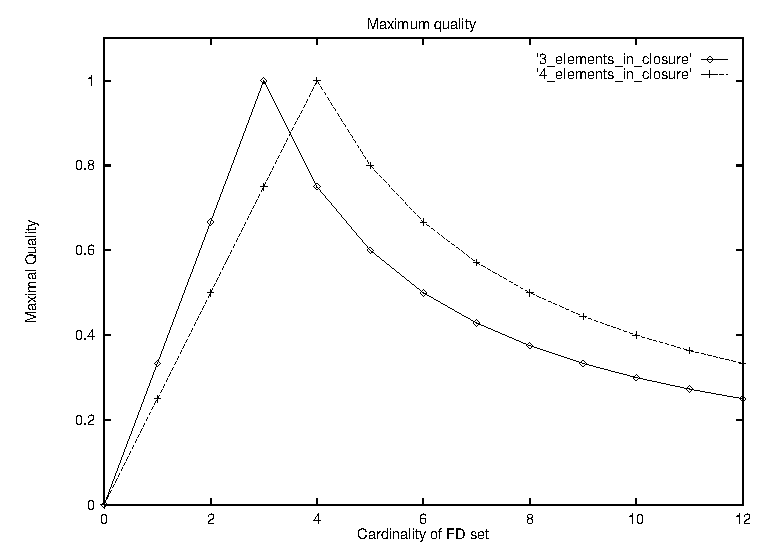
\includegraphics{figures/qual2.eps}}}
\caption{\label{graph:simquality}{Max Quality for FD sets with 3 and 4
elements in closure}}
\end{figure}

\begin{definition}[Similarity Measure]
\begin{rm}
Given two sets of FDs, F and G over R, we define the measure of
their similarity as:
\begin{displaymath}
sim({\rm F}, {\rm G}) = \frac{\mid {\rm CL(F)} \cap {\rm CL(G)} \mid}{\mid {\rm CL(F)} \cup {\rm CL(G)} \mid }\quad\quad\Box
\end{displaymath}
\end{rm}
\end{definition}

We now seek to characterise the monotonicity properties of $sim$ with respect
to F and G. In equation~\ref{eq:f_xy} we consider the maximum
possible values of $sim$ where one FD set F is fixed, containing $n$
elements in CL(F). Any other FD set G
containing $k$ elements in CL(G) has a maximal quality, 
if all FDs in G are in F
whenever $k \le n$, and if all FDs in F are in G whenever $k > n$.
In Figure~\ref{graph:simquality} we show 
these variations for two fixed FD sets with 3 and 4 respective
elements in their closure.

\begin{equation}\label{eq:f_xy}
sim_F({\rm G}) = \left\{ \begin{array}
		{l@{\quad:\quad}ll}
\frac{n}{k} & n \le k & \quad\mbox{when}\quad {\rm G}^\star \supseteq
		{\rm F}^\star\\ 
\frac{k}{n} & n > k   & \quad\mbox{when}\quad {\rm F}^\star \supset
		{\rm G}^\star\\ 
			\end{array}	\right.
\end{equation}

The similarity measure is monotonically increasing and if a {\em
core}, or intersection, of the two FD sets is
increased by two different amounts, $m$ and $k$, where $m \le k$, then
the value of similarity is larger for the larger core size
increase. We now define some axioms of this similarity measure:
\begin{enumerate}
\item $sim({\rm F}, {\rm F}) = 1$
\item $sim({\rm F}, {\rm G}) = sim({\rm G}, {\rm F})$
\item $sim({\rm F}, {\rm G}) = 0$, if F$^\star \cap G^\star = \emptyset$
\item $sim({\rm F}, \emptyset) = 0$
\item $sim({\rm F}, {\rm G}) = \frac{|{\rm CL(F)}|}{ |{\rm CL(G)}|}$, if F$^\star \subseteq$ G$^\star$
\item  $sim({\rm F},{\rm G}) \le sim({\rm G},{\rm H})$ if F
$\subseteq$ H and H $\Delta$ F $\in$ G. 
\end{enumerate}

Information concerning related similarities can now be formed. Assume we
have three sets of FDs, F, G, and H, and that F is
fixed. Now, if $sim_{\rm F}$(G) = 0 and 0 $<$ $sim_{\rm F}$(H) $<$ 1
then we know 
that $sim({\rm G},{\rm H}) <$ 1 given that there is a similarity between F and
H. Essentially, this is stating that the core of F and H cannot 
form any part of the core of G and H. Using 
knowledge of the measure itself allows for inferences to be drawn
easily based on the input FD set and resulting values of the
measure. We have briefly
presented an overview of a similarity measure for FD sets. In
Chapter~\ref{chap:numdep} we define a metric based on the lattice
properties of NDs, used within our work on indefinite relations.

\subsection{Relational Database Sampling Procedures}\label{subsec:dat_samp}
\index{Sampling}
\index{Sample Size}
\index{PAC-learning}

Many real-world databases are too large to consider applying standard
data mining algorithms to. Therefore, as a solution, sampling from
such databases has been promoted \cite{km94,toi96b}. Samples drawn
from a large database are mined for dependencies which are then
associated with error and confidence thresholds based on the size of
the sample in relation to the database. Alternatively, results
obtained from the mining of a sample may be verified against the
database as a whole. In this manner sampling is a necessary trade-off
between accuracy and efficiency of results.

\medskip

\cite{km94} addresses the problem of finding a suitable sample
size. This is presented within a PAC-learning framework
\cite{val84}. Based on an error measure, akin to the similarity
measure presented in Section~\ref{subsec:rev_fd_sim} or $g_3$ of
Table~\ref{tbl:fd_approx},  sampling is used to detect all sentences
which have an 
error (or 1 - similarity) less than a given threshold
$\epsilon$. The probability that at least one sentence with an error
greater than $\epsilon$ will not be formed is given by $\delta$, the
confidence parameter. FDs which hold are, obviously, never detected as
false. \cite{toi96b} presents sampling within an exact discovery
framework for association rules using a sample to find a superset of
frequent associations subsequently verified by one pass over the
database.


\subsection{Resampling in Statistics}\label{subsec:res_in_stat}
\index{Resampling}
\index{Bootstrap Resampling}
\index{Bootstrap Resampling!example}
Statistical methods have evolved rapidly over
the last 30 years, not least due to the harnessing of increasing
computational power.  In the 70's statistical modelling was based upon
decomposing the data into a structure and noise.  In the 80's
non-parametric 
processes such as the {\em jackknife} were developed where $n$ or more
(possibly) correlated estimates of the quantity of interest are
replaced by pseudovalues. Linear regression takes a linear combination
of the available values whereas non-parametric models keep the data
around and use it for estimating the response class of a new point.


The bootstrap \cite{efro79,de83,et93} is a data driven
simulation method for estimating the sampling distribution of a
statistic. It is a computationally 
intensive procedure that has been shown to provide good results which
would not have been capable of being readily generated more than 30 years ago.
In our experience, resampling has not previously been 
applied to solve database problems such as the consistency problem.
Declining computational cost is altering the face of statistical analysis
entailing a domino effect in other fields so that computer
intensive statistical methods such as the bootstrap will become much
more prominent in many areas of computer science over the next few years.
Figure~\ref{rev:bootstrap} shows how the
bootstrap procedure may be applied to an indefinite relation $r$. The
sample in the figure will consist of $n$ possible worlds, each
satisfying an ND set. We now introduce bootstrap resampling with a
simple example; resampling indefinite relations is formalised in
Chapter~\ref{chap:consistency}. 

\begin{figure}[ht]
\centerline{\scalebox{0.7}{{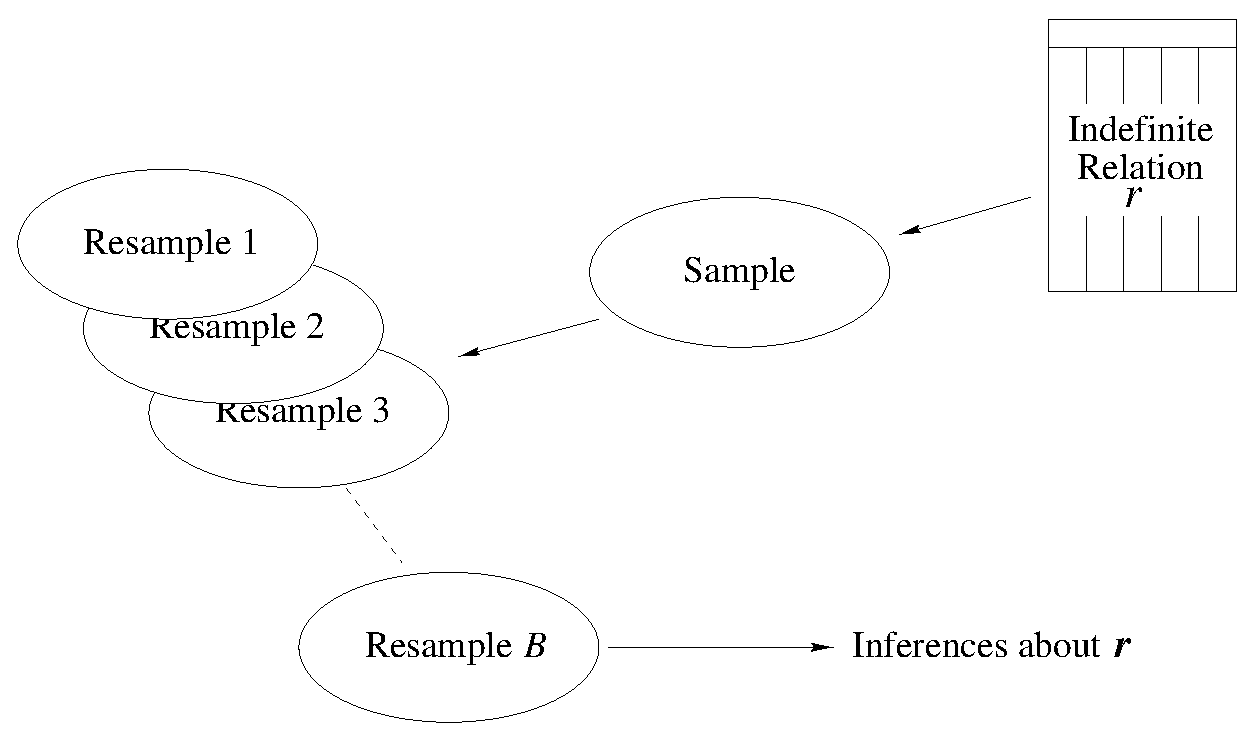
\includegraphics{review/bootstrap.eps}}}}
\caption{\label{rev:bootstrap} The Bootstrap Procedure as applied to an
indefinite relation with a Bootstrap Replication size (BRS) $B$}
\end{figure}

The following example is used for instruction and is similar
to one described in \cite{et93} but with a business 
application.
If we have a relation depicting the number of pension plan subscribers
(referred to as Clients) in 
two different companies with a number of the employees in
each company as in Table~\ref{table:3.01} then we can form a ratio of
success $\hat{\theta}$ based on the number of clients 
for the respective number of employees, given as follows:

\begin{displaymath}
\hat{\theta} = \frac{230 / 15746}{299 / 13430} = 0.66
\end{displaymath}

{\line
\begin{table}[ht]
\begin{center}
\begin{tabular}{|c|c|c|} \hline
Company & Clients & Employees \\ \hline
HAL co.	& 230		& 15746 \\
JCN co. & 299 		& 13430 \\ \hline
\end{tabular}
\end{center}
\caption{\label{table:3.01} Company Data Relation}
\end{table}
}

So we can say that HAL co. is only 66\% as successful as JCN co. when
 it comes to getting employees to take up its pension plan. Yet
this is only an estimated ratio. To apply a bootstrap procedure to
the above data we can create two sample populations for each
company with 230 clients and
(15746 - 230) employees and 299 clients and (13430 - 299) employees,
 respectively. These populations of 15746 and 13430 items may be
 represented with ones and zeros to represent clients and
 employees who are not clients.
If we then draw randomly with replacement a sample of 15746 subjects and 13430
 subjects from each population
we can form what is known as a bootstrap replicate sample success ratio
$\hat{\theta^\star}$. We can now repeat this, say, 1000 times, to
obtain bootstrap standard deviation values or other statistics which are based
on the distribution found and not naive assumptions on the distribution.

\smallskip

The majority of bootstrap applications in the statistical domain use
resampling due to the unavailability of the complete domain. Likewise,
in an indefinite relation, although we potentially have access to all
possible worlds, there are generally too many to examine them all. We
employ resampling in a dynamic manner on increasing sample sizes,
elaborated upon in Chapter~\ref{chap:consistency}. 

\section{Discussion}


Within the limits of our experience, there has
been no work on the data mining of relations containing indefinite
information, possibly due to the lack of availability of indefinite data.
Catalytic relations, introduced in \cite{HS95}, those that are
essentially the join of 
two or more relations, provide a possible avenue for indefinite
information data mining if the join performed does not create the
cartesian product but instead creates disjunction within cells which
do not agree on their attributes, referred to in
Section~\ref{subsec:tl_catdm}. 

\medskip

The work of \cite{Via87,Via88} was seminal in the field of temporal
dependencies. Possible extensions discussed herein for NDs
in~\ref{subsec:temdat} warrant
further study. Nearly all work on dependency mining
\cite{Mann92,km95,sf93,bb95,hkp98} presents studies of the efficiency
of dependency mining, frequently noting that large number of
dependencies were discovered in relations. For example, \cite{sf93}
reports the discovery of 1191 FDs in a relation with 471 tuples over
17 attributes. Obviously the majority of these FDs discovered will
be near trivial due to large left hand side attribute sets functioning as
keys. We remark that there has been little work assessing the
real value of FD discovery in the data mining process. Such
potentially meaningless FDs also motivate the use of a user supplied
template to 
define FD approximations to dependencies which the user is interested
in.  

\medskip

From the work of \cite{mt96,bt98} we note the required restriction to
simple pattern discovery otherwise an NP-complete problem is
faced. Therefore it is necessary to restrict the discovery process. We
choose, in Chapters~\ref{chap:templog} and~\ref{chap:tempresult}, to
restrict our discovery to patterns which correspond to temporal
properties \cite{mp92}. We cite the work of
\cite{dlm98} and \cite{bt98} as having closely related goals to our
own work though 
their methodologies are different.






\chapter{Numerical Dependencies in Databases and Data
Mining}\label{chap:numdep} 

We now concentrate on introducing Numerical Dependencies (NDs) and
related theoretical and practical issues so that we are fully able to
appreciate later work utilising NDs in indefinite and temporal
relations.

\medskip

Initially, in Section~\ref{sec:nd_approx} we formalise the lattice
of NDs. We also show how ND values may be {\em uninformative} for a given
relation and define {\em mean} NDs to combat such
problems. Section~\ref{sec:nd_chase} introduces the chase for NDs as a
precursor to the chase for NDs in indefinite relations in
Chapter~\ref{chap:consistency}. We discuss and extend the ND 
axiomatisation of \cite{gm85a} in Section~\ref{sec:nd_inf}
and show that the chase for NDs as an inference procedure
is sound and complete.
An algorithm for data mining of NDs in
Section~\ref{sec:nd_datamine} is presented with respect to related
work. Section~\ref{sec:nd_evolve} discusses, 
briefly, an evolutionary algorithm for database design presented
in \cite{cl98c}, which uses NDs within a hill-climbing
procedure. We conclude with a general overview of
this chapter and its implications for data mining in
Section~\ref{sec:nd_disc}, together with a note on possible Armstrong
relations for NDs.


\section{Approximating FDs with NDs}\label{sec:nd_approx}
\index{Numerical Dependencies!{to Approximate FDs}}
We now define the lattice of NDs and then show how this may be
used to form a metric for approximating proximity to a given FD set. 

\subsection{The Lattice of NDs}
\index{Lattice of NDs}
\index{Lattice Theory|see{Lattice of NDs}}
Firstly, we present the lattice of NDs. We begin with
Definition~\ref{def:more} which is then used to define the lattice of
NDs and Definition~\ref{def:covered} which is used in our algorithm
for climbing the lattice.

\index{NDs!more functional set}
\begin{definition}[More functional set of NDs]\label{def:more}
\begin{rm}
A set of NDs $N_1$ over R is {\em more functional} than a set of NDs 
$N_2$ over R, denoted by $N_2 \sqsubseteq N_1$, whenever
X $\to^{k_2}$ Y $\in N_2$ if and only if \linebreak \protect{X $\to^{k_1}$ Y $\in
N_1$} and  
\protect{$k_1 \le k_2$}. $\quad\Box$
\end{rm}
\end{definition}

The set-theoretic relation, more functional than, 
is a partial order in the sets of NDs.
Assume that we are considering only sets of NDs over a schema R which
are more functional  
than a given set of NDs, N over R, each of the form X $\to^k$ Y, 
for some $k \ge 1$.
Then the family of sets of NDs that are more functional than N form a lattice
whose bottom element is N and whose top element is the set of FDs
induced by N, i.e. \{X $\to$ Y $\mid$ X $\to^k$ Y $\in$ N\}.
The {\em least upper bound}, $lub$, of $N_1$ and $N_2$ is the set of NDs
\{X $\to^{min(k_1, k_2)}$ Y $\mid$
X $\to^{k_1}$ Y $\in N_1$ and X $\to^{k_2}$ Y $\in N_2$\},
where $min(k_1, k_2)$ is the minimum of $k_1$ and $k_2$, and the 
{\em greatest lower bound}, $glb$, of $N_1$ and $N_2$ is defined similarly using maximum.
We call the lattice, whose top element is the set of FDs F over R
and whose bottom element is the set of NDs
\{X $\to^m$ Y $\mid$ X $\to$ Y $\in$ F\}, ${\cal L}_m$(F)
(or simply ${\cal L}_m$ if F is understood from context), with $m \ge 1$.


Therefore, we can {\em approximate} a set of FDs F by a set of NDs N
such that N $\sqsubseteq$ F. 
The {\em closer} N is to F in ${\cal L}_m$ the better the approximation is.
From now on we let ${\cal L}_m$ 
{\em be the lattice of NDs whose top element is} F
and, for a relation $r$, assume that $\mid r \mid = m+1$, with $m \ge 1$. In
Figure~\ref{latt:1} we present a lattice for two NDs whose attributes
are not specified, over a relation with a maximum domain size of 4 in
the right hand side of each ND. The lattice size significantly increases
with more NDs and larger domain sizes.
The probability of
an ND $X \to^k Y$ being satisfied in a relation $r$ tends to one as
$k$ gets closer to $\mid r \mid - 1$. 
\index{Numerical Dependency!Covered By}
\begin{definition}[Covered By]\label{def:covered}
\begin{rm}
We say that $N_2$ is {\em covered by} $N_1$, denoted by $N_2$ $\cover$
$N_1$, where $N_1, N_2 \in {\cal L}_m$, 
if $N_1 \not= N_2$, $N_2 \sqsubseteq N_1$ and
$\forall N^\prime \in {\cal L}_m$ such that 
$N_2 \sqsubseteq N^\prime \sqsubseteq N_1$ we have $N^\prime =
N_2$. $\quad\Box$ 
\end{rm}
\end{definition}

\begin{figure}[ht]
\centerline{\scalebox{0.55}{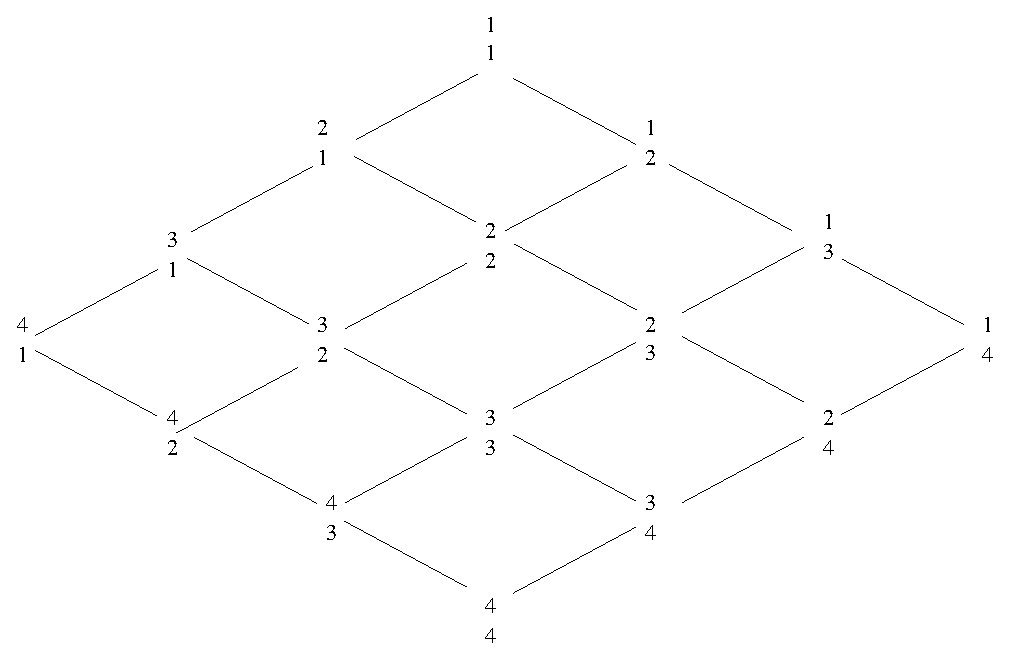
\includegraphics{figures/latt1.eps}}}
\caption{\label{latt:1}Lattice of NDs for a relation of 2 FDs
(not shown) and maximum domain size of 4 for each dependency}
\end{figure}

\index{Numerical Dependency!Maximal Set}
\begin{definition}[Maximal set of NDs]
\begin{rm}
The {\em maximal} set of NDs of $r$ with respect to F,
denoted by $maximal(r$, F), is the maximal set N of NDs
in ${\cal L}_m$(F) (with respect to $\sqsubseteq$) such that $r
\models$ N.$\quad\Box$ 
\end{rm}
\end{definition}
\medskip

Given $r$ and F, $maximal(r$, F) can be computed in polynomial time in the
sizes of $r$ and F by a straightforward hill climbing procedure
on ${\cal L}_m$(F), illustrated in algorithm~\ref{alg:mu}. For each X $\to$ A $\in$ F this procedure finds 
the minimal $k$ such that $r \models$ X $\to^k$ A, starting 
from X $\to^m$ A which $r$ trivially satisfies since $\mid r \mid = m$. 

\index{Numerical Dependencies!improvement set}
\begin{definition}[Improvement set of a set of NDs]
\begin{rm}
The {\em improvement set} of $r$ with respect to F, 
denoted by $\mu$($r$, F), is defined as 
\begin{displaymath}
\mu(r, {\rm F}) = \{{\rm X} \to^k {\rm A} \mid 
{\rm X} \to^k {\rm A} \in maximal(r, {\rm F}) \mbox{ and }  k > 1\}.
\end{displaymath}
Algorithm~\ref{alg:mu} returns the {\em improvement set} of $r$ if any FDs
satisfied in $r$ are removed from N.$\quad\Box$
\end{rm}
\end{definition}
\medskip


{\renewcommand{\baselinestretch}{1}
\begin{figure}[ht]
\begin{center}
\fbox{\begin{minipage}{14cm}
\begin{algorithm}[{\rm MU}($r$, {\rm F})]\label{alg:mu}
\begin{rm}
\begin{tabbing}
t1\=t2\=t3\=t4\=t5\= \kill \\
1.  \> \> {\bf begin} \\
2.  \> \> \> $m$ := $\mid r \mid$; \\
3.  \> \> \> N := the bottom element of $\mathcal{L}_m$ (F); \\
4.  \> \> \> {\bf while} $\exists$ G such that N $\cover$ G {and} $r \models$ G  {\bf do} \\
5.  \> \> \> \> N := G; \\
6.  \> \> \>  {\bf end while} \\
7. \> \> \> {\bf return} N;  \\
8. \> \> {\bf end.}
\end{tabbing}
\end{rm}
\end{algorithm}
\end{minipage}}
\end{center}
\caption{\label{numdep:fig:mu} The improvement algorithm for NDs}
\end{figure}
}

\subsection{Similarity Measures and Numerical Dependencies}
\index{Similarity Measure!ND}

We introduce a measure for calculating the proximity of two ND sets using
their position within the lattice.  We show that this measure is a distance
function, satisfying reflexivity and symmetry, and is also a metric, 
satisfying the triangle inequality. Firstly, we begin by defining the best
approximation given by a set of NDs to their functional counterparts.
We define the {\em size} of a set of NDs N to be the number of attributes 
appearing in N including repetitions and define a {\em step}, either up
or down, to be exactly minus or plus one, respectively, to a single branch of
one ND within an ND set. 

\begin{definition}[The best approximation of a set of FDs]\label{def:best}
\begin{rm}
A set of NDs N over R is the {\em best approximation} of 
a set of FDs F over R with respect to a relation $r$ over R,
with $\mid r \mid = m+1$ (or simply the best approximation of F
if $r$ is understood from context), if $r \models$ N 
and there does not exist a set of NDs, $N^\prime \in {\cal L}_m$
such that N $\cover$ $N^\prime$ and $r \models N^\prime$.$\quad\Box$
\end{rm}
\end{definition}



\begin{proposition}[The number of NDs higher in the Lattice]
\begin{rm}
Given an ND set $N$ = \linebreak[4]   $\{ X_1 \to^{k_1} A_1, X_2 \to^{k_2} A_2,
 \ldots, X_n \to^{k_n} A_n \}$, the number of ND sets above this set in the
lattice is ($k_1 \cdot k_2 \cdot \ldots \cdot k_n$) - 1.
\end{rm}
\end{proposition}

{\em Proof.} An ND is higher in the lattice if within a 
set of NDs none of the $k_i$ branches have any values higher than
any of those in the set {\em and} at least one of the NDs has some 
$k_j$ branch value
lower than one of those in the set. Each ND $X_i \to^{k_i} A_i$ within
the set can take $k_i$ values. We consider all permutations of these
values to get $k_1 \cdot k_2 \cdot \ldots \cdot k_n$ from which we 
must ensure that the ND set values of $N$ itself is not included to get
$k_1 \cdot k_2 \cdot \ldots \cdot k_n$ - 1. $\Box$

\smallskip

This provides us with the basis for a distance measure between an ND set
and its functional representation. However,  using this technique allows,
in some instances, ND sets which are the same number of steps below the
FD equivalent to have different values. This is due to ND sets containing
FDs or NDs which are close to being functional having less sets above them
in the lattice. To illustrate, if we have two ND sets $N_1,N_2$ each containing two NDs such that $N_1$ has dependencies with 4 and 2 as branches whilst $N_2$ has dependencies with 3 and 3 as branches then $N_1$ will have fewer ND sets
above it in the lattice though both are the same number of steps from their
functional equivalent, shown in Figure~\ref{latt:1}. We now introduce the 
metric we used in our simulations
and note that if we are interested in comparing ND sets with either more 
or less {\em near} FDs we can refer to the above measure 
whenever the metric provides the same distance.
\smallskip

In the following definition {\em distance} is defined as the number of
{\em steps} in the lattice. In Definition~\ref{def:nd_prox} we
use proposition~\ref{prop:maxdist} to prove that the denominator for
this measure is normalised for any two NDs within a given
relation. $p(N_1,N_2)$ provides a suitable measure of proximity
between two ND sets. We use the measure of
Definition~\ref{def:nd_prox} in our simulations presented in
Chapter~\ref{chap:consistency} in the following form: Given a set of NDs $N_1$ and a set of FDs $F$, which $N_1$ approximates,
then the proximity between the two dependency sets is given by
$p(N_1,F)$. 
\index{Numerical Dependency!Proximity measure}
\begin{definition}[Proximity between two ND sets]\label{def:nd_prox}
\begin{rm}
Given two sets of NDs $N_1$ and $N_2$ we define the metric as follows: 
\[
p(N_1,N_2) = \frac{\Sigma_{i = 1, 2} \mbox{ Distance from } N_i \mbox{ to }  lub \{ N_1, N_2 \}}
{\mbox{Maximum distance between any two ND sets to their $lub$ in the lattice}}
\quad\Box\]
\end{rm}
\end{definition}

We define the bottom of the
lattice to be the set of NDs with each branching factor equivalent to
the domain size of the attribute on the right hand side of each
ND, assuming a finite domain size.

\smallskip
\begin{proposition}\label{prop:maxdist}
\begin{rm}
The maximum distance between any two points in
the lattice to their $lub$ is always equivalent to the
distance from the bottom to the top of the lattice. 
\end{rm}
\end{proposition}

{\em Proof}. We prove this by induction on the NDs within the two ND sets.\newline 
\smallskip
\indent ({\em Basis}): We see that if $N_1$ and $N_2$ are empty then the
result is immediate.

\smallskip

({\em Induction}): We have two ND sets $N_1$ and $N_2$ which are distance
$d$ apart where $d \le q$ and $q$ is the maximum distance apart between
any two ND sets. We add an ND $X \to^{k_1} Y$
to $N_1$ and $X \to^{k_2} Y$ to $N_2$ which differ only
on their branching factor. Without loss of generality, if $k_1 < k_2$ then the
distance apart between $N_1$ and $N_2$ becomes $d + k_2 - k_1$. This 
remains less than or equal to the maximum distance apart which is $q + k'_2 -
k'_1$ where, without loss of generality, $k'_1 = 1$ (it is an FD) and
$k'_2$ is at the bottom of the lattice. $\Box$

\smallskip

The measure $p$ is a distance function given that the distance
between two NDs is zero only when they are equivalent and that 
$p(n_1,n_2) = p(n_2,n_1)$ always holds. It also satisfies the 
triangle inequality, whose proof we now outline. This implies
therefore that $p$ is a metric implying that sets with a common value
can be compared.

\begin{theorem}
\begin{rm}
Given three ND sets, $N_1$, $N_2$, and $N_3$, $p(N_1,N_2) + p(N_2,N_3)
\ge p(N_1,N_3)$.
\end{rm}
\end{theorem}
\smallskip

{\em Proof.} We show that if $N_1$, $N_2$ and $N_3$ are non-empty and the 
triangle
inequality holds then the addition of a new ND to each set which may
differ only on its branching factor will still satisfy the triangle inequality.
Assume we add three NDs $X \to^{k_i} A$ with $i = 1,2,3$ to $N_1,N_2$ and
$N_3$, respectively. We also assume, without loss of generality, that 
$k_1 < k_3$. We denote each ND set $N_i \cup \{ X \to^{k_i} A \}$ by $N'_i$
for $i = 1,2,3$. We perform induction on the NDs in each set.

\smallskip
({\em Basis}): If $N_1$ = $N_2$ = $N_3$ = $\emptyset$ then the 
result is immediate.

\smallskip
({\em Induction}):
 We assume that $k_2 \le k_1$, then $p(N'_1,N'_2)$ =
distance from $N_1$ to $lub(N_1,N_2)$ + distance from $N_2$ to $lub(N_1,N_2)$ +
$k_2 - k_1$. Similarly for $p(N'_2,N'_3)$ and $p(N'_1,N'_3)$ we have the
additional components, $k_3 - k_2$ and $k_3 - k_1$. Therefore, we have
$p(N'_1,N'_2) + p(N'_2,N'_3)$ = $p(N_1,N_2) + k_1 - k_2 + p(N_2,N_3) +
k_3 - k_2$ and $p(N'_1,N'_3)$ = $p(N_1,N_3) + k_3 - k_1$. We know that  
$p(N_1,N_2) + p(N_2,N_3) \ge p(N_1,N_3)$ holds and we see
 that  $k_1 - k_2 + k_3 - k_2 \ge k_3 - k_1$ holds if $k_1 \ge k_2$ which
is true, based on our initial assumption. We can similarly prove the 
triangle inequality for the case when $k_1 \le k_2$. $\Box$


\subsection{Partitioning a Relation for Mean NDs}\label{nd:subsec:mean}
\index{Numerical Dependency!Mean ND}
In many data mining tools it is important that there exist measures
which accurately reflect the content of the database; this motivates
us to define mean ND set satisfaction for some situations like that of
Example~\ref{ex:mean_nd}.

\smallskip

In Chapter~\ref{chap:review} we presented Definition~\ref{def:nd_part}
for partitioning of a relation into blocks for an ND X $\to^k$ Y which
agree on X.
The satisfaction of an ND X $\to^k$ Y implies only that there exists
at least one partition ${\cal B}$ which contains at least $k$ tuples
with at most $k$ different Y-values.  There may however be numerous
other partitions on X which may have far less than $k$ different
Y-values and so the partition ${\cal B}$ dominates the relation and
presents an inaccurate representation of the proximity to FD set
satisfaction.  We therefore define the {\em mean numerical dependency}.

\index{Numerical Dependency!Mean ND}
\index{Mean ND}
\begin{definition}[Mean Numerical dependency]\label{def:mean_nd}
\begin{rm}
A {\em mean numerical dependency} over R (or simply a mean ND)
is a statement of the form X $\to^{\bar{k}}$ Y, where X, Y $\subseteq$ R and
$\bar{k} \ge 1$. We refer to $\bar{k}$ as the {\em mean branching
factor}.$\quad\Box$ 
\end{rm}
\end{definition}
\index{Mean ND!Satisfaction}
\begin{definition}[Satisfaction of a Mean ND]\label{def:sat-mean_nd}
\begin{rm}
Let $r$ be a relation over R.
An ND X $\to^{\bar{k}}$ Y is {\em satisfied} in $r$,
denoted by $r \models$ X $\to^{\bar{k}}$ Y, such that $r$ is
partitioned into blocks 
$\{{\cal B}_1, {\cal B}_2, \ldots, {\cal B}_w\}$ with respect to X
$\to$ Y such that $\bar{k} = \frac{\sum_{i = 1}^{w} \mid
\pi_{\rm Y}({\cal B}_{i}) \mid }{w}$.
A set of averaged NDs $\bar{\rm N}$ is {\em satisfied} in $r$,
denoted by $r \models$ $\bar{\rm N}$, whenever
$\forall$ X $\to^{\bar{k}}$ Y $\in$ $\bar{\rm N}$, $r \models$ X
$\to^{\bar{k}}$ Y.$\quad\Box$ 
\end{rm}
\end{definition}



\begin{example}\label{ex:mean_nd}
\begin{rm}
We assume that a relation $r$ over AB satisfies the ND A $\to^{14}$ B
as its closest approximation to the FD A $\to$ B. However $r$ may, for
example, only
contain three partitions $\{{\cal B}_1, {\cal B}_2, {\cal B}_3\}$
with each partition satisfying the NDs A $\to^{14}$ B, A $\to^{1}$ B,
and A $\to^{1}$ B, respectively. We note the last two are satisfied
functionally. The mean ND set satisfaction is A $\to^{\bar{5.67}}$ B.
Within a block $\cal B$ the number of tuples is not related to
the branching factor value, given by $\mid \pi_{\rm B}({\cal B}) \mid$.
\end{rm}
\end{example}

In our work on indefinite information in relations we remark that we
are interested in exact ND set satisfaction only, given the nature of
the problem. In the data mining of NDs in standard and temporal
relations we may often be interested in the mean ND set satisfaction
value. We note that if this value is vastly different from the exact
satisfaction value then it is likely that one or more partitions from
the relation {\em dominate} and remaining partitions will satisfy the
NDs more functionally.

\section{The Chase Procedure for NDs}\label{sec:nd_chase}
\index{Chase Procedure!for NDs}

We now show how CHASE($r$, F) can be generalised to CHASE($r$, N), where N is
a set of NDs over R, shown in Figure~\ref{numdep:fig:nd_chase}.

{\renewcommand{\baselinestretch}{1}
\begin{figure}[ht]
\begin{center}
\fbox{\begin{minipage}{16cm}
\begin{algorithm}[{\rm CHASE}($r$, {\rm N})]\label{alg:ndchase}
\begin{rm}
\begin{tabbing}
t1\=t2\=t3\=t4\=t5\=t6\=t7\= \kill \\
\ra.  \> \> {\bf begin} \\
\sa.  \> \> \> Result := $r$; \\
\sa.  \> \> \> Tmp := $\emptyset$; \\
\sa.  \> \> \> {\bf while} Tmp $\not=$ Result {\bf do} \\
\sa.  \> \> \> \> Tmp := Result; \\
\sa.  \> \> \> \> {\bf if} $\exists$ X $\to^k$ Y $\in$ N, $\exists t_1, t_2, \ldots, t_k, t_{k+1} \in$ Result such that  \\
    \> \> \> \> \> $t_1$[X] = $t_2$[X] = $\ldots$ = $t_k$[X] = $t_{k+1}$[X] \\
    \> \> \> \> \> but $t_1$[Y] $\not=$ $t_2$[Y] $\not= \ldots \not=$ $t_k$[Y] $\not=$ $t_{k+1}$[Y] {\bf then} \\ 
\sa. \> \> \> \> \> {\bf for each} $A \in$ Y$-$X {\bf do} \\
\sa. \> \> \> \> \> \> \> $t_i$[A],$t_j$[A] := max($t_i$[A],$t_j$[A])
    for two distinct values $i,j \in 1,\ldots,k+1$; \\
\sa. \> \> \> \> \> {\bf end for} \\
\sa.  \> \> \> \> {\bf end if} \\
\sa.  \> \> \> {\bf end while} \\
\sa. \> \> \> {\bf return} Result;  \\
\sa. \> \> {\bf end.}
\end{tabbing}
\end{rm}
\end{algorithm}
\end{minipage}}
\end{center}
\caption{\label{numdep:fig:nd_chase} The Chase procedure for NDs}
\end{figure}
}

We leave it to the reader to verify that when $k = 1$, i.e. X $\to^k$ Y is an
FD, then CHASE($r$, N) reduces to CHASE($r$, F).


\begin{lemma}\label{th:algterm}
\begin{rm}
Algorithm~\ref{alg:ndchase} terminates.
\end{rm}
\end{lemma}

{\em Proof.} No new values are introduced into the algorithm at any
step and therefore the algorithm must halt after executing the while
loop a finite number of times. $\Box$

\begin{theorem}\label{th:chase}
\begin{rm}
Given a set of NDs, N, then $\forall n \in N$, CHASE($r$, N) $\models n$.
\end{rm}
\end{theorem}

{\em Proof.} Direct from the definitions of the algorithm and of ND
satisfaction. $\Box$

We also note in theorem~\ref{th:chase} that if $r \models$ N, for a
relation $r$ and an ND set N then \linebreak CHASE($r$, N) = $r$.
We return to the chase procedure and show how it can be used as an
inference procedure in Section~\ref{subsec:nd_ch_inf}, after discussion of the
axiomatisation of NDs.   

\section{Inferences for Numerical Dependencies}\label{sec:nd_inf}

The axiom system given in \cite{gm85a} is shown to be sound and
complete only in the special cases of, for a schema R, either $|$R$| \le 3$ or when the number of
NDs with $k > 1$ is at most one. \cite{gm85b} extends this result
and shows that there is no finite sound and complete
axiomatisation for NDs. 

\subsection{ND Axiomatisation}\label{subsec:nd_axiom}
\index{Numerical Dependency!Axiomatisation}
\index{Numerical Dependencies!Inference Rules}
NDs allow a more general dependency relation than functional
dependencies.  \cite{gm85a,gm85b} introduce NDs with regard
to obtaining normal forms which avoid or minimise redundancy, from a
database with $k$-dependency constraints. Grant and Minker also
provide an axiomatisation for NDs which is a
generalisation of the Armstrong axioms for 
FDs. \cite{gm85a} presents a set of sound
inference rules for NDs. \cite{gm85b} 
shows that there does not exist a {\em finite} set of sound and
complete inference rules for Numerical Dependencies.
These axioms are shown to be complete for relations which have, at most,
3 attributes.  It is shown that any relation with more than 3 attributes is
not complete. We show in Section~\ref{subsec:nd_ch_inf} how the chase may
be used as an inference procedure.
If the relation utilises only FDs then the axioms
contain the Armstrong rules as a subset.\\

For clarity, we now present inference rules 1-5 from \cite{gm85b}:
\begin{description}
\item[R1] If Y $\subseteq$ X then infer X $\to$ Y
\item[R2] From X $\to^k$ Y infer ZX $\to^k$ ZY
\item[R3(a)] From X $\to^k$ Y and Y $\to^j$ Z infer X $\to^{k \cdot j}$ YZ
\item[R3(b)] From X $\to^k$ Y and Y $\to^j$ Z infer X $\to^{k \cdot j}$ Z
\item[R4] From X $\to^k$ Y infer X $\to^{k + 1}$ Y
\item[R5$_m$] From  $\{ X \to^{2} Y_i \quad |  \quad 1 \le i \le 3m-2
\}$  \\
$\quad \cup$ $\quad \{ Y_{i1}Y_{i2} \ldots Y_{im} \to Z
\quad |  \quad 1 \le i1 < i2 < \ldots < im \le 3m-2 \}$ infer $X \to^{2} Z$
\end{description}

Rules R1,R2 and R3(b) are extensions of the axioms for FDs.
We now present another inference rule which generalises the rule
R5$_m$ of \cite{gm85b}, R6$_{k,m}$, which can be viewed as a generalised
transitivity rule for NDs wherein a bound on the number of attributes
required for inference is created based on the branching factor of the
NDs {\em and} the number of attributes on the left hand side of the FD
which determines attribute $Z$. R6$_{k,m}$ is a useful extension to
the class of transitive axioms for NDs.

\smallskip
{\line
\begin{table}[ht]
\begin{tabular}{cl} \\
(R6$_{k,m}$): 	& From  $\{ X \to^{k} Y_i \quad |  \quad 1 \le i \le
		\eta \}$    $\quad \cup$ \\
		&    $\quad \{ Y_{i1}Y_{i2} \ldots Y_{im} \to Z
		\quad |  \quad 1 \le i1 < i2 < \ldots < im \le \eta \}$ \\ 
\rule{0cm}{5mm} & we can infer $X \to^{k} Z$ where $\eta =
		(m-1){k+1 \choose 2} + 1$  \\
\end{tabular}
\end{table}}
\smallskip

\begin{theorem}\label{th:1}
\begin{rm}
Each rule R6$_{k,m}$ is sound and has minimal hypothesis.
\end{rm}
\end{theorem}

{\line
\begin{table}[ht]
\begin{center}
\begin{tabular}{|c|c|c|c|c|c|} \hline
X	&	Y$_i$	&	Y$_2$	& $\ldots$ & Y$_{\eta}$	 & Z \\\hline
1	&		&		&          &	       & 1 \\
1	&		&		&          &	       & 2 \\	
$\vdots$ &		&		&          &	       & $\vdots$ \\
1	&		&		&          &	       & $k+1$\\ \hline
\end{tabular}
\end{center}
\caption{\label{tbl:axiom_r6km} Example relation for proof of axiom R6$_{k,m}$}
\end{table}}	


{\em Proof.} We assume that we have a relation $r$ with $\eta + 2$
attributes and $k+1$ cells, as in Table~\ref{tbl:axiom_r6km}, and that
X agrees on all of its $k+1$ cells.  We also assume, from 
R6$_{k,m}$, that X $\to^k$ Y$_i$ holds for all $1 \le i \le \eta$ and
that for a given $m$ all possible FDs of the form \linebreak Y$_{i1}$Y$_{i2}$ $\ldots$
Y$_{im}$ $\to$ Z hold for 1 $\le i1 < i2 < \ldots < im \le \eta$ and
that X $\to^k$ Z does not hold.
Each X $\to^k$ Y$_i$ implies that each Y$_i$ attribute must agree on
at least two cells. In a relation with $k + 1$ tuples there are 
${k+1 \choose 2}$ ways in which a single
attribute may agree on two tuples. For some set of attributes
Y$_{i1}$Y$_{i2}$ $\ldots$ Y$_{im}$ 
in Y$_1$ to Y$_{\eta}$ if $\eta = (m-1){k+1 \choose 2} + 1$, then at
least one FD of the form \linebreak Y$_{i1}$Y$_{i2}$ $\ldots$
Y$_{im}$ $\to$ Z must agree on all of its Y$_i$ attributes. This is due to
exhaustion of all possible combinations on which two tuples may agree.
Whichever tuples agree on all $m$ attributes imply that Z also agrees
on these attributes. Therefore there may not be $k+1$
different values on Z and we have a contradiction. 
\medskip

We prove the minimal hypothesis by noting that if any FD X $\to^k$ Y
or \linebreak Y$_{i1}$Y$_{i2}$ $\ldots$
Y$_{im}$ $\to$ Z for 1 $\le i1 < i2 < \ldots < im \le \eta$ is
omitted from our requirements then there exists a counterexample which
does not imply X $\to^k$ Z for some combination of values on the
attributes in Y$_1$ to Y$_{\eta}$. $\Box$

\smallskip

We can also prove this as for R5$_m$ in \cite{gm85b} by explicitly
proving that no counterexample relation exists.
We note that when $k$ = 1 then R6$_{k,m}$ reduces to transitivity of FDs,
and when $k$ = 2 then $\eta = 3m - 2$, the figure given in
\cite{gm85b} for R5$_m$. 


\subsection{The Chase as an Inference Procedure}\label{subsec:nd_ch_inf}
\index{Chase Procedure!for ND inference}

We prove that the chase is a 
sound and complete inference procedure for NDs. In the sequel, we
assume that NDs have singleton right hand sides.

Given a set of NDs $N$ and an ND $\sigma$, we apply the chase as an
inference tool to discover if $N \models \sigma$. 
We create a relation $r_\sigma$ which for $\sigma = X \to^k
A$ has $k+1$ tuples with $k+1$ different values on attribute set $A$,
all values on X equivalent and all values in $R \backslash XA$ unique.
We need to consider all possible iterations of the chase procedure,
presented in algorithm~\ref{alg:ndchase}, for a relation $r_\sigma$
for the inference procedure to be sound and complete, given that one
instance of the chase may not terminate with a unique end result,
known as the {\em Church-Rosser} property \cite{mms79}. We refer to
each complete application of the chase as a {\em chase sequence}.

{\line
\begin{table}[ht]
\begin{center}
\begin{tabular}{c|c|c|c|c|c|c|c|} \cline{2-8}
 		& X$_1$ 	& $\ldots$ 	& X$_m$ & A 	& B$_1$ & $\ldots$ 	& B$_m$ \\ \cline{2-8}
$t_1$ 		& 1  		& $\ldots$ 	& 1	&  1  	& 1 	& $\ldots$ 	& 1 \\
$t_2$ 		& 1  	& $\ldots$ 	& 1&  2  	& 2 	&  $\ldots$ 	& 2 \\
$\vdots$ 	& $\vdots$  &  $\ddots$ & $\vdots$  &  $\vdots$  & $\vdots$ & $\ddots$ & $\vdots$ \\
$t_{k+1}$ 	& 1  &  $\ldots$  &  1  & $k+1$  & $k+1$ & $\ldots$ 	& $k+1$ \\ \cline{2-8}
\end{tabular}
\end{center}
\caption{\label{tbl:rel_chase1} Relation to be chased by ND set N with
$\sigma = X \to^k A$, X = $\{ X_1, \ldots, X_m \}$, R $\backslash$ XA = $\{ B_1, \ldots, B_m \}$
and $m$ = $|$ R $\backslash$ XA $|$}
\end{table}}	


We motivate theorem~\ref{th:3} by showing an example relation where
different sequences of tuples modified by the chase produce different
results. We show this for an ND set \linebreak N = $\{$ X $\to^2$ 
B$_1$,  X $\to^2$ B$_2$, B$_1$B$_2$ $\to$ A $\}$, $\sigma$ = X $\to^2$
A, and relation $r_1$ in
Table~\ref{tbl:NDchase1}. 
 For two different chase sequences, with different tuples modified, we have
$r_{1}^c$ 
$\not\models$ X $\to^2$ A, shown in Table~\ref{tbl:NDchase2}, and $r_{1}^c$ 
$\models$ X $\to^2$ A, shown in Table~\ref{tbl:NDchase4}.
Therefore 
N $\not\models$  X $\to^2$ A, which may not have been discovered if
we had only examined one chase sequence.

{\line
\begin{table}[ht]
\begin{center}
\begin{tabular}{|c|c|c|c|} \hline
 {\bf X} & {\bf B$_1$} & {\bf B$_2$} & {\bf A} \\\hline
 1 & 1 & 1 & 1 \\ 
 1 & 2 & 2 & 2 \\ 
 1 & 3 & 3 & 3 \\ \hline
\end{tabular}
\end{center}
\caption{\label{tbl:NDchase1}$r_1$ before CHASE procedure} 
\end{table}
}

{\line
\begin{table}[ht]
\begin{minipage}[b]{7cm}
\begin{center}
\begin{tabular}{|c|c|c|c|} \hline
 {\bf X} & {\bf B$_1$} & {\bf B$_2$} & {\bf A} \\\hline
 1 & 1 & 2 & 1 \\ 
 1 & 3 & 2 & 2 \\ 
 1 & 3 & 3 & 3 \\ \hline
\end{tabular}
\end{center}
\caption{\label{tbl:NDchase2}Example CHASE($r_1$,N) after CHASE procedure} 
\end{minipage}
\hfill
\begin{minipage}[b]{7cm}
\begin{center}
\begin{tabular}{|c|c|c|c|} \hline
 {\bf X} & {\bf B$_1$} & {\bf B$_2$} & {\bf A} \\\hline
 1 & 1 & 1 & 1 \\ 
 1 & 3 & 3 & 3 \\ 
 1 & 3 & 3 & 3 \\ \hline
\end{tabular}
\end{center}
\caption{\label{tbl:NDchase4}Counterexample CHASE($r_2$,N) after CHASE procedure } 
\end{minipage}
\end{table}
}


Theorem~\ref{th:2} requires the notion of containment mapping
cf. \cite{atze93}.  We define a function $dom$ which
returns the active domain of a relation.

\begin{definition}[Containment Mapping]\label{def:cm}
\begin{rm}
A containment mapping $\phi$ from $r_\sigma$ to a relation $r$ has
each value in $dom$($r_\sigma$) mapped by $\phi$ to a value in $dom$($r$).
This is extended to tuples over $R = A_1A_2 \ldots A_m$ as $\phi(t) =
\phi(t[A_1]),\phi(t[A_2]),\ldots, \phi(t[A_m])$ and extends to a
relation as $\phi(r) = \{ \phi(t) | t \in r \}$.$\quad\Box$ 
\end{rm}
\end{definition}


\begin{theorem}\label{th:2}
\begin{rm}
Given a set of Numerical Dependencies N and a ND $\sigma = X \to^k A$,
N $\models \sigma$ iff $\neg\exists t^c_1[A] \not= t^c_2[A] \not= \ldots
\not= t^c_{k+1}[A]$ where $t^c_1,t^c_2,\ldots,t^c_{k+1} \in
r_\sigma^c$ and $r_\sigma^c$ = chase($r_\sigma$,N) for all possible
sequences of the chase.
\end{rm}
\end{theorem}

\index{Soundness!of the chase for NDs}
\index{Completeness!of the chase for NDs}

{\em Proof. (if)} We assume that $A \not\subseteq X$. We let $r$ be a
relation over $R$ such that $r \models N$; we show that $r \models
\sigma$. Let $t_1, t_2, \ldots, t_{k+1} \in r$ such that $t_1[X] =
t_2[X] = \ldots = t_{k+1}[X]$. We claim that for some $i,
j \in \{1, 2, \ldots, {k+1}\}$ there exists $t_i[A] = t_j[A]$. 

\smallskip
Let $\phi$ be a containment mapping from $r_\sigma$
$\phi(u_1) = t_1$, $\phi(u_2) = t_2$, $\ldots$, $\phi(u_{k+1}) = t_{k+1}$. We
shall prove that $\phi$ is additionally a containment mapping from
CHASE($r_{\sigma}$, N) to $r$ so that for some $i,j \in r_{\sigma}^c$,
$\phi(t_i^c[A])$ = $\phi(t_j^c[A])$ implies $t_i[A] = t_j[A]$. This is
the case for all possible chase sequences on $r_\sigma$. 

\smallskip
We prove this by induction on the number of steps, $s$, required to compute
CHASE($r_{\sigma}$, N).

\smallskip

({\em Basis}):
If $s = 1$ then for some ND $W \to^k B \in N$ two values are equated 
in $B$ where \linebreak $W \subseteq X$ and $A = B$ so therefore $u_i[A] =
u_j[A]$ implying that $\phi(u_i[A]) = t_i[A]$ and \linebreak $\phi(u_j[A]) =
t_j[A]$ and so $t_i[A] = t_j[A]$ for some $i,j$ in $r$.
\smallskip
 
({\em Induction}):
We assume that the result holds when $s$ steps of the chase procedure
are required. We now prove it to be true when $s+1$ chase steps are
required. We let the $s+1$ chase step be for an ND $W \to^k B$ and
$u_i, u_j$ be two tuples in $r_\sigma$ such that the $s+1$ step either modifies
$u_i$ or $u_j$. Thus, for $B$ either $u_i[B]$ or 
$u_j[B]$ is modified so that $u_i[B] = u_j[B] = t_i^c[A] = t_j^c[A]$.
Now, given $u_i[W] = u_j[W]$ then $\phi(u_i[W]) = \phi(u_j[W])$ by the
definition of containment mapping.  Therefore $\phi(t_i^c[A]) =
\phi(t_j^c[A]) = \phi(u_i[B]) = \phi(u_j[B]) = t_i[A] = t_j[A]$ holds, since $r_{\sigma}
\models W \to^k B$. Given that $\phi$ only differs from the result of
$s$ steps on $u_i[B]$ or $u_j[B]$ it is a containment mapping from
$r_\sigma^c$ in all possible chase sequences. In any sequence, if
$t_i^c[A] = t_j^c[A]$ we have, by definition of $\phi$, $t_i[A] = t_j[A]$.

\smallskip

{ \em (only-if)} If, in some chase sequence, there does not exist
$t_i^c[A] = t_j^c[A]$ for 
some $i,j \in {1,2, \ldots, k+1}$ then we can
construct a relation $r$ 
which satisfies all $n \in N$ but violates $\sigma$.  
\smallskip
Alternatively, the chase for $r_\sigma$ can be shown to be isomorphic
to a relation $r$ which satisfies N but violates X $\to^k$ A by
mapping each value in $r_{\sigma}^c$ to a value in $dom(r)$. $\Box$



\begin{corollary}\label{th:3}
\begin{rm}
The chase inference procedure for Numerical Dependencies is sound and
complete.
\end{rm}
\end{corollary}

{\em Proof.} Soundness and completeness of the chase as an inference
procedure is a corollary of theorem~\ref{th:3}. $\Box$

\smallskip
The existence of a sound and complete chase procedure shows that
implication on NDs is decidable. The implication
problem for NDs is in co-NP, used to denote that the complementary
no/yes problem is in the 
set NP \cite{gj79}; we know that the converse
problem is NP given that we can {\em guess} a relation  (equivalent to
a complete sequence of the chase procedure) 
$r_\sigma^c$ 
and verify in polynomial time whether or not
$r_\sigma^c$ $\models$ $\sigma$. NP-completeness remains an open problem.


\subsection{Armstrong Relations for NDs}\label{subsec:nd_ar}
\index{NDs!Armstrong Relations for}

Within a finite relation there does not exist an
Armstrong Relation, defined for FDs in Definition~\ref{def:AR}, for a
set of NDs N, unless N contains all possible 
combinations of attribute sets. We may prove this as follows. Assume that we
are given a set of NDs N and that $\sigma$ is an ND X $\to^k$ Y such that
N $\not\models \sigma$. For any relation $r$ such that $r \models$ N we
have, at least, $r \models \sigma$ where $k = \mid r \mid$.

\medskip
We therefore define a weak AR for an ND set N.
\index{Armstrong Relations!for NDs}

\begin{definition}[A Weak Armstrong Relation]\label{def:weak_AR}
\begin{rm}
A relation $r$ is a weak AR for a set of NDs N if $r \models$ N and
$\forall \sigma$ such that N $\not\models \sigma$ then $r \models
\sigma$ maximally 
with respect to $k_\sigma$ implying that $r$ satisfies all NDs
$\sigma$ with a branching 
factor no higher than $k_\sigma$. The choice of a value for $k_\sigma$
may be related to branching factors of NDs in N (or the size of the
relation).$\quad\Box$ 
\end{rm}
\end{definition}

These weak Armstrong Relations would extend the practical application
of NDs within database design tools by helping designers think of what
NDs may be required via examination of an actual relation. 

\section{Numerical Dependencies in Data Mining}\label{sec:nd_datamine}
\index{Numerical Dependency!in data mining}
We now briefly present data mining for numerical dependencies in
standard relations. We emphasise the following:
\begin{itemize}
\item In contrast with functional dependency approximation data mining
we are not seeking to assess what proportion of a relation satisfies a
functional relationship, cf. Table~\ref{tbl:fd_approx} and
\cite{hkp98,km95}. We seek to discover 
generalisations of FDs when the FD may be viewed as too strict.
\item In our work on temporal and indefinite relations we assume the
user provides a ND set upon which we seek instances of ND
satisfaction. The use of NDs in a blind discovery context would
generate ND satisfying instances for all possible attribute set
combinations, which is not practical due to the complexity.
\end{itemize}

\subsection{Dependency Mining Applications}\label{subsec:fd_jobs}
\index{Dependency Data Mining!using NDs}
Approximation of the dependency set, possibly approximated using numerical
dependencies, on a large database in existence may reveal unknown information
in the form of these dependencies which may hold in the database. A
recent work on the reverse-engineering, or discovery if you will, of
cardinality constraints for inference of the ER-model is presented in
\cite{sou98}. From lemma~\ref{rev:lem_cc} this is another application
for ND discovery.

\smallskip

Applications for dependency mining include a database
design tool which the database designer can use in conjunction with a possible
instance of the data to be stored within the database.  Inference upon this 
example set will then provide the designer with vital information as to possible
unknown dependencies that be satisfied in the relation. The approach of 
Bell and Brockhausen \cite{bb95} in making inferences from the verified and
invalid data dependencies is aimed at {\em supporting} the database
designer. Example~\ref{nd:ex_nd_app} shows an application of ND discovery.


\begin{example}\label{nd:ex_nd_app}
\begin{rm}
In a patient database within a hospital every patient visit is
independently stored within a {\em patient} details relation and a {\em
disease/symptom/treatment} relation.  
Given a numerical dependency specified $DISEASE \to^{10} SYMPTOM$ stating
that a disease can have at most 10 symptoms, it may however be approximated
that $ADDRESS \: \: \: PATIENT \to^{6} SYMPTOM$ showing that at most
6 of the symptoms can occur at the same location for a patient.
\end{rm}
\end{example}


\subsection{Mining a relation for a set of NDs}

We consider only singleton right hand sides. For a relation $r$ over R with
$n$ attributes we have $n 2^{n-1}$ NDs returned by this algorithm and
so in Figure~\ref{graph:nd_mine1} we only give results obtained from
restricting the 
left hand sides to a given arity of 
attributes. Algorithm~\ref{alg:mine} uses Algorithm~\ref{alg:mu} to
generate the ND satisfied from an FD template.

\medskip

{\renewcommand{\baselinestretch}{1}
\begin{figure}[ht]
\begin{center}
\fbox{
\begin{minipage}{16cm}
\begin{algorithm}[{\rm ND\_mine}($r$, {\rm R})]\label{alg:mine}
\begin{rm}
\begin{tabbing}
t1\=t2\=t3\=t4\=t5\=t6\=t7\=t8\=t9\= \kill \\
\ra.  \> \> {\bf begin} \\
\sa.  \> \> \> ND\_set := $\emptyset$;\\
\sa.  \> \> \> {\bf for each} A $\in$ R {\bf do}\\
\sa.  \> \> \> \> {\bf for each} W $\in \mathcal{P}$(R - A) {\bf do}\\
\sa.  \> \> \> \> \> $\{$ W $\to^k$ A $\}$ =  MU($r$, $\{$ W $\to$ A $\}$); \\
\sa.  \> \> \> \> \> ND\_set := ND\_set $\cup$ $\{$ W $\to^{k}$ A $\}$; \\
\sa. \> \> \>  \> {\bf end for}; \\
\sa. \> \> \>    {\bf end for}; \\
\sa. \> \> \> {\bf return} ND\_set;  \\
\sa. \> \> {\bf end.}
\end{tabbing}
\end{rm}
\end{algorithm}
\end{minipage}}
\end{center}
\caption{\label{numdep:fig:nd_mine} The ND mining algorithm}
\end{figure}
}

The computational complexity of algorithm~\ref{alg:mine} is O($n^2 2^{n-1}
\mid r \mid log \mid r \mid$). There are $n2^{n-1}$ possible NDs and
it takes time O($n \mid r \mid log \mid r \mid$) to sort a relation into
partitions. We can restrict the arity of the left hand side to a size
$m$ or even restrict to singleton left and right
hand sides where we have a time of O($n^3\mid r \mid log \mid r \mid$).
When the lhs of any ND is $\emptyset$ then the ND corresponds
directly to the domain size.
The scale of the mining can be cut down by using axioms provided
in \cite{gm85b,gm85a} when exact details are not required for
dependencies of the form $W \to^k A$ where $W = YV$ and we already
know $Y \to^{k_1} A$ and $V \to^{k_2} A$ which would give $k \le k_1$
or $k \le k_2$, depending on the larger partition. 

\medskip

It is also possible that we could use the chase procedure for NDs to
further improve the efficiency of the algorithm such that for a set of NDs
N we do not mine for an ND $\sigma$ if N $\models \sigma$.

\begin{figure}
\centerline{\scalebox{0.7}{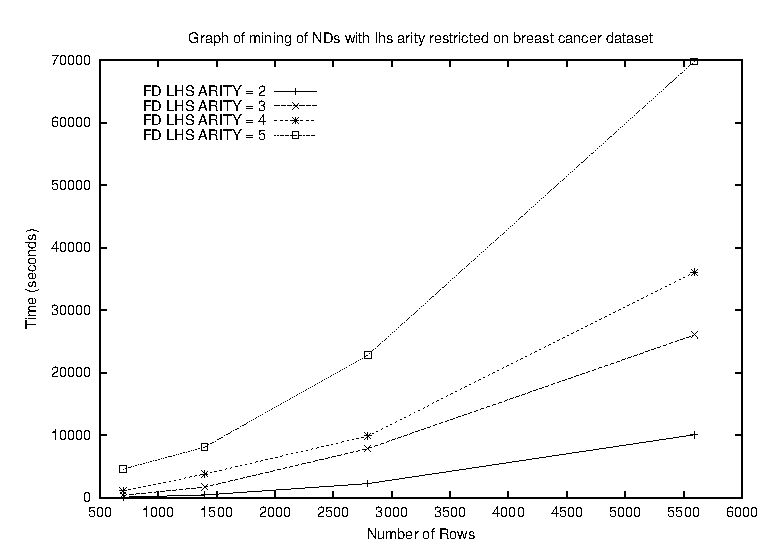
\includegraphics{figures/nd_mine_bc.eps}}}
\caption{\label{graph:nd_mine1}{Results for mining Mean and
standard NDs with arity of the lhs of each ND restricted upon the
breast cancer dataset}}
\end{figure}

In Figure~\ref{graph:nd_mine1} we see how increases in the arity of
the left side of the NDs increase the time required to mine for sets
of NDs in increasing relation sizes. The time increases represent the
additional overhead of more dependencies due to more possible
attribute combinations on the left hand side of NDs, with respect to
the complete attribute set, and the time to compare additional
attributes for insertion into partitions. We have applied this to the
breast cancer data set \cite{bkm98} used in many data mining research
papers. The data set has 11 attributes and 699 tuples. We increase
these tuples by adding identifiers to each tuple and copying (as used
by \cite{hkp98}). Obviously in a relation with 11 attributes 
there is little point in examining the powerset of attributes as it is
highly likely that an FD with, say 7 or more, attributes on the left hand
side will be satisfied functionally and will be meaningless. This
point is reiterated in \cite{sf93}. 

\subsection{Mining a relation for a set of Mean NDs}

The time to mine for a set of mean NDs is the same as for standard
NDs given that we need to examine each partition as before.
The difference between the satisfied mean NDs and the standard ND
satisfaction may tell us much about the dataset which we highlight in
Example~\ref{ex:bc_mean}.

\begin{example}\label{ex:bc_mean}
\begin{rm}
In the breast cancer database there is an attribute {\em
marginal\_adhesion} with a domain of 10 elements. The ND $mitosis$
$\to^{10}$ $marginal\_adhesion$ tells
us only that there is at least one partition containing all 10
elements on an attribute value of
$mitosis$. The mean ND $mitosis$ $\to^{\bar{5.67}}$
$marginal\_adhesion$ tells us most partitions have fewer elements.
\end{rm}
\end{example}


\section{Evolving Example Relations to Satisfy FDs}\label{sec:nd_evolve}
\index{Evolutionary Algorithm}
\index{Example Relation}
\index{Evolving Example Relations}
We now briefly present an example of applying NDs to approximate FDs
in an evolutionary hill-climbing algorithm for creating probabilistic
example relations for use within database design applications. This
work summarises \cite{cl98}, and, as indicated in
Section~\ref{subsec:reldbdes}, is related to work in the
Design-By-Example project of \cite{mr86}.

\smallskip

Example relations satisfying a given set of integrity constraints such as 
FDs are important during the database design 
activity in order to guide the designer towards the specification of a correct 
set of constraints for the application in hand \cite{sm81}. 



\subsection{Motivation}

If the example relation shown to the database designer is too large then 
the designer will {\em not} be able to assimilate all the knowledge embedded in
that relation. Thus it would be useful to be able to generate random examples 
relations that satisfy F and whose maximal cardinality is specified by the 
database designer; in general, such an example may not be an Armstrong
relation.

\smallskip

Our algorithm is evolutionary in that it incorporates a stochastic approach
for altering a relation by a {\em mutation} operation.
 The algorithm proceeds as
follows; initially a relation is randomly generated following
the input of the designer and a given FD set. This relation is then
 mutated based on a probabilistic selection of an unsatisfied FD  from the
given set and an attribute which assists violation of this FD in the relation.
We use NDs as an
approximation of the unsatisfied FDs in the relation. 
The mutations steer the relation
towards a final state wherein all of the FDs in the specified set are
satisfied. It is a simple algorithm, and indeed a basic tenet 
of evolutionary programming is to create algorithms 
which do not constrain evolution too severely,
 much like organic evolution \cite{bs93}. All evolved relations are then mined 
using a quality function, defined in~\ref{subsec:rev_fd_sim}, whose criterion is exact satisfaction of the given FD set. 

\smallskip

A deterministic approach used to generate an Armstrong relation
(Algorithm 14.2, \cite{Mann92}) has the severe drawback
 in that the same relation
is generated every time the algorithm runs.  Our probabilistic
approach is advantageous in that different example relations may
be generated from equivalent domain sizes and the tuple size may be
increased or decreased by the designer as desired. Moreover, as long as 
the number of tuples exceed the minimum size required for an Armstrong relation
 \cite{bdfs84,mr86} then one may 
be returned, although this is not guaranteed.  Below this number and a
deterministic approach fails 
 whereas our evolutionary approach complies with the desires of the user
and returns a relation which, if selected from a batch or {\em 
population} of evolutions, is likely to be as high a quality
as possible given the domain and tuple restriction.  From the user's
point of view it may often be highly beneficial to examine a smaller
relation of a high quality, but less than one, as opposed to a larger Armstrong
relation (with a quality of one).
Simulations
emphasised the validity of this approach within database
design, showing that many varying relations can be efficiently
evolved for an FD set with numerous domain and tuple inputs.
 They also showed that it is extremely useful to know the quality of an
 example relation, and additionally that Armstrong
relations are often formed within a batch. 



\index{Randomised Algorithm}
\subsection{Mutating relations}
\index{Mutating relations}
\label{sec:mutate}

Herein, we present an algorithm for {\em mutating} a relation.
Informally, given a relation which does not satisfy F, MUTATE($r$, F) 
randomly selects an ND, say X $\to^k$ A, in the improvement set of $r$ and 
stochastically modifies some of the tuple values in $r$.
We then define the syntactic property of non-interfering NDs 
and show that if the selected ND and another ND
Y $\to^g$ C in $maximal(r$, F) are {\em non-interfering}, see Definition~\ref{def:nd_non-int} then, after the mutation, 
$r$ will still satisfy Y $\to^g$ C.
The non-interference property is important,
since if we evolve a relation to satisfy a set of FDs by iterating the
mutation operation, then the evolution process will be more efficient 
when the NDs in $maximal(r$, F) are non-interfering.

\medskip

The {\em mutation} of a relation over R with respect to a set of FDs over R 
denoted by MUTATE($r$, F), is defined as the relation resulting from invoking 
Algorithm~\ref{alg:mutate} presented below. In this algorithm we use LHS
 to denote the left hand side of an ND and RHS to denote the right hand
side.  This random selection of a side removes any bias which might otherwise
have been incurred if the selection of an attribute to mutate were
taken over the whole ND, given that the left hand side may be any
length less than or equal to $\mid$ R $\mid$ but the right hand side is
always singleton. $\mathcal{D}$ denotes the domain of values in the
relation $r$.


{\line
\begin{figure}[ht]
\begin{center}
\fbox{\begin{minipage}{11cm}
\begin{algorithm}[{\rm MUTATE}($r$, {\rm F})]\label{alg:mutate}
\begin{rm}
\begin{tabbing}
t1\=t2\=t3\=t4\=t5\= \kill \\
1. \> \>{\bf begin}\\
2. \>\> \> Result := $r$;\\
3. \>   \>\> Uniformly randomly select an ND X $\to^k$ A $\in$ MU($r$,
F) with $k > 1$;\\
4. \>   \>\> Uniformly randomly select a tuple $t \in r$;\\
5.  \> \>  \>{\bf if} $r[$X, $t[$X$]] \models$  X $\to^{k - 1}$ A  {\bf then}\\
6.  \> \> \>\> {\bf return} $r$;\\
7.\> \> \>{\bf end if} \\
8.  \> \>\>Uniformly randomly select RHS or LHS of ND \\
9.  \> \>   \>{\bf if} LHS {\bf then}\\
10. \> \>  \>\> Uniformly randomly select an attribute B $\in$ X\\
11. \> \>   \> \>Uniformly randomly select a value $v \in \mathcal{D} - \{t[$B$]\}$; \\
12. \> \> \> {\bf else} \% B = A\\
13. \> \> \> \> B := A;\\
14. \> \> \>\>  Uniformly randomly select a value $v \in \pi_{\mbox{\small{A}}}(r[$X,$t[$X$]]) - \{t[$A$]\}$; \\
15.  \> \> \>{\bf end if} \\
16. \> \> \>{\bf for each} $u \in r[$X, $t[$X$]]$ such that $u[$XA$] = t[$XA$]$  {\bf do}\\
17.\> \> \> \> $u[$B$]$ := $v$;\\
18. \> \> \>{\bf end for} \\
19. \> \> \> {\bf if} Result $ \models$  X $\to^k$ A  {\bf then}\\
20.  \> \> \>\> {\bf return} Result;\\
21. \> \> \>{\bf else}\\
22. \> \> \>\> {\bf return} $r$;\\
23. \> \> \>{\bf end if}\\
24.  \>  \> {\bf end. }
\end{tabbing}
\end{rm}
\end{algorithm}
\end{minipage}}
\end{center}
\caption{\label{numdep:fig:mutate} The MUTATE procedure for evolving relations}
\end{figure}
}
\medskip
The following definition provides us with a measure of how useful a mutation 
is in the evolution of a relation to satisfy a set of FDs.

\begin{definition}[Useful, neutral and damaging mutations]
\begin{rm}
Let $s$ be the relation resulting from the mutation MUTATE($r$, F).
Then a mutation such as $s$ is said to be {\em useful}, {\em neutral} or 
{\em damaging}, respectively, for an ND Y $\to^g$ C,
if the number of blocks ${\cal B}_i$
in the partitioning of $s$ with respect to Y $\to^g$ C
such that ${\cal B}_i \not\models$ Y $\to^g$ C
is less than, equal to or greater than, respectively, 
the number of blocks ${\cal B}_i$ 
in the partitioning of $r$ with respect to Y $\to^g$ C
such that ${\cal B}_i \not\models$ Y $\to^g$ C. $\quad\Box$
\end{rm}
\end{definition}

\index{Numerical Dependencies!non-interfering}
\begin{definition}[Non-interfering NDs]\label{def:nd_non-int}
\begin{rm}
Two NDs X $\to^k$ A and Y $\to^g$ C are said to be {\em non-interfering} if 
either A = C and Y = X, or YC $\cap$ XA $= \emptyset$, 
or A $\not=$ C, X = C and YC = R.$\quad\Box$
\end{rm}
\end{definition}
\medskip

We call a set of NDs N over R such that every pair of FDs in N is
non-interfering a {\em non-interfering} set of NDs.
An attribute B in the left-hand side of an FD X $\to$ A is said to be 
{\em redundant} with respect to a set of FD F over R, if A $\in$ (X$-$B)${}^+$.
Assuming that no left-hand sides of FDs in F have redundant attributes,
it can be shown that when X $\to^k$ A is the ND chosen at line 3 of 
Algorithm~\ref{alg:mutate}, then the probability that any mutation MUTATE($r$, F)
is neutral for Y $\to^g$ C $\in maximal(r$, F), is at least 1 / $\mid$XA$\mid$.
At times, it is necessary to accept mutations that are damaging 
to some of the NDs in N. 

\medskip


\begin{theorem}\label{theorem:neutral}
\begin{rm}
Assuming that X $\to^k$ A is the ND chosen at line 3 of 
Algorithm~\ref{alg:mutate}, then for all relations $r$ over R,
any mutation MUTATE($r$, F) is neutral for Y $\to^g$ C $\in maximal(r$, F),
if and only if X $\to^k$ A and Y $\to^g$ C are non-interfering NDs.
\end{rm}
\end{theorem}

{\em Proof.} We prove this by considering all possible relationships
between XA and YC in example relations, given in \cite{cl96}. \newline

{\em If.} 
The only nontrivial case to consider is when A $\not=$ C, X = \{C\} and YC = R,
implying that A $\in$ Y. If the attribute chosen for mutation is A,
then equating two or more A-values is neutral for Y $\to^g$ C, since the 
C-values of the all the tuples, $u \in$ $r$[X, $t$[X]], are equal. 
On the other hand, if the attribute chosen for mutation is C, 
then forcing two or more C-values to be unequal is neutral for Y $\to^g$ C, 
since there can only be one tuple in $r$ having the same YC-values
due to the fact that YC = R.

\medskip
{\em Only if.} 
We prove the result by contraposition, considering the various cases.

\smallskip

{\em Case 1.1.}
Suppose that A = C and X and Y are incomparable,
i.e.  X $\not\subseteq$ Y and Y $\not\subseteq$ X.
Let X be the singleton B, Y be the singleton D,
and $r$ be the relation over ABD, shown in Table~\ref{tbl1}.
Then, it can easily be verified that 
$r \not\models$ B $\to$ A but $r \models$ D $\to$ A.
On the other hand, the relation $s$ shown in Table~\ref{tbl2},
which is a mutation resulting from MUTATE($r$, F) assuming that 
B $\to^2$ A is the ND chosen at line 3 of Algorithm~\ref{alg:mutate},
is damaging for D $\to$ A, since $s \not\models$ D $\to$ A.

\begin{table}[ht]
\begin{minipage}[b]{7cm}
\begin{center}
\begin{tabular}{|c|c|c|} \hline
A & B & D \\ \hline
0 & 0 & 1 \\
1 & 0 & 0 \\
1 & 1 & 0 \\ \hline
\end{tabular}
\end{center}
\caption{\label{tbl1} Example relation for Case 1.1.} 
\end{minipage}
\hfill
\begin{minipage}[b]{7cm}
\begin{center}
\begin{tabular}{|c|c|c|} \hline
A & B & D \\ \hline
0 & 0 & 1 \\
0 & 0 & 0 \\
1 & 1 & 0 \\ \hline
\end{tabular}
\end{center}
\caption{\label{tbl2} A mutation of $r$ shown in Table~\ref{tbl1}} 
\end{minipage}
\end{table}

{\em Case 1.2.}
Suppose that A = C and Y $\subset$ X, i.e. Y is a proper subset of X.
Let Y be the singleton B, X = DB,
and $r$ be the relation over ABD, shown in Table~\ref{tbl3}.
Then, it can easily be verified that 
$r \not\models$ DB $\to$ A but $r \models$ B $\to^2$ A.
On the other hand, the relation $s$ shown in Table~\ref{tbl4},
which is a mutation resulting from MUTATE($r$, F) assuming that 
DB $\to^2$ A is the ND chosen at line 3 of Algorithm~\ref{alg:mutate},
is damaging for B $\to^2$ A, since $s \not\models$ B $\to^2$ A.

\begin{table}[ht]
\begin{minipage}[b]{7cm}
\begin{center}
\begin{tabular}{|c|c|c|} \hline
A & B & D \\ \hline
2 & 0 & 0 \\
0 & 0 & 0 \\
0 & 1 & 1 \\ 
1 & 1 & 1 \\ \hline
\end{tabular}
\end{center}
\caption{\label{tbl3} Example relation for Case 1.2.} 
\end{minipage}
\hfill
\begin{minipage}[b]{7cm}
\begin{center}
\begin{tabular}{|c|c|c|} \hline
A & B & D \\ \hline
2 & 1 & 0 \\
0 & 0 & 0 \\
0 & 1 & 1 \\ 
1 & 1 & 1 \\ \hline
\end{tabular}
\end{center}
\caption{\label{tbl4} A mutation of $r$ shown in Table~\ref{tbl3}} 
\end{minipage}
\end{table}

{\em Case 1.3.}
Suppose that A = C and X $\subset$ Y, i.e. X is a proper subset of Y.

Let X be the singleton B, Y = DB,
and $r$ be the relation over ABD, shown in Table~\ref{tbl5}.
Then, it can easily be verified that 
$r \not\models$ B $\to$ A but $r \models$ DB $\to$ A.
On the other hand, the relation $s$ shown in Table~\ref{tbl6},
which is a mutation resulting from MUTATE($r$, F) assuming that 
B $\to^2$ A is the ND chosen at line 3 of Algorithm~\ref{alg:mutate},
is damaging for DB $\to$ A, since $s \not\models$ DB $\to$ A.

\begin{table}[ht]
\begin{minipage}[b]{7cm}
\begin{center}
\begin{tabular}{|c|c|c|} \hline
A & B & D \\ \hline
0 & 0 & 0 \\
1 & 0 & 1 \\ 
1 & 1 & 0 \\ \hline
\end{tabular}
\end{center}
\caption{\label{tbl5} Example relation for Case 1.3.} 
\end{minipage}
\hfill
\begin{minipage}[b]{7cm}
\begin{center}
\begin{tabular}{|c|c|c|} \hline
A & B & D \\ \hline
0 & 1 & 0 \\
1 & 0 & 1 \\ 
1 & 1 & 0 \\ \hline
\end{tabular}
\end{center}
\caption{\label{tbl6} A mutation of $r$ shown in Table~\ref{tbl5}} 
\end{minipage}
\end{table}

{\em Case 2.1.}
Suppose that A $\not= C$, X $\not=$ \{C\} and YC = R; 
in this case C $\in$ X may or may not hold.
Let X be either the singleton B or X = BC, Y = AB.
and $r$ be the relation over ABC, shown in Table~\ref{tbl7}.
Then, it can easily be verified that 
$r \not\models$ BC $\to$ A 
but $r \models$ AB $\to$ C.
On the other hand, the relation $s$ shown in Table~\ref{tbl8},
which is a mutation resulting from MUTATE($r$, F) assuming that either
B $\to^2$ A or BC $\to^2$ A is the ND chosen at line 3 of 
Algorithm~\ref{alg:mutate},
is damaging for AB $\to$ C, since $s \not\models$ AB $\to$ C.

\begin{table}[ht]
\begin{minipage}[b]{7cm}
\begin{center}
\begin{tabular}{|c|c|c|} \hline
A & B & C \\ \hline
0 & 0 & 0 \\
1 & 0 & 0 \\ 
0 & 1 & 1 \\ \hline
\end{tabular}
\end{center}
\caption{\label{tbl7} Example relation for Case 2.1.} 
\end{minipage}
\hfill
\begin{minipage}[b]{7cm}
\begin{center}
\begin{tabular}{|c|c|c|} \hline
A & B & C \\ \hline
0 & 1 & 0 \\
1 & 0 & 0 \\ 
0 & 1 & 1 \\ \hline
\end{tabular}
\end{center}
\caption{\label{tbl8} A mutation of $r$ shown in Table~\ref{tbl7}} 
\end{minipage}
\end{table}

{\em Case 2.2.}
Suppose that A $\not= C$, X = \{C\} and YC $\not=$ R. 
Let X be the singleton A, Y be the singleton C,
and $r$ be the relation over ABC, shown in Table~\ref{tbl9}.
Then, it can easily be verified that 
$r \not\models$ C $\to$ A but $r \models$ A $\to$ C.
On the other hand, the relation $s$ shown in Table~\ref{tbl10},
which is a mutation resulting from MUTATE($r$, F) assuming that 
C $\to^2$ A is the ND chosen at line 3 of Algorithm~\ref{alg:mutate},
is damaging for A $\to$ C, since $s \not\models$ A $\to$ C.

\begin{table}[ht]
\begin{minipage}[b]{7cm}
\begin{center}
\begin{tabular}{|c|c|c|} \hline
A & B & C \\ \hline
0 & 0 & 0 \\
1 & 0 & 0 \\ 
0 & 1 & 0 \\ \hline
\end{tabular}
\end{center}
\caption{\label{tbl9} Example relation for Case 2.2.} 
\end{minipage}
\hfill
\begin{minipage}[b]{7cm}
\begin{center}
\begin{tabular}{|c|c|c|} \hline
A & B & C \\ \hline
0 & 0 & 1 \\
1 & 0 & 0 \\ 
0 & 1 & 0 \\ \hline
\end{tabular}
\end{center}
\caption{\label{tbl10} A mutation of $r$ shown in Table~\ref{tbl9}} 
\end{minipage}
\end{table}

{\em Case 2.3.}
Suppose that A $\not= C$, X = \{C\} and A $\not\in$ Y. 
Let Y be the singleton D,
and $r$ be the relation over ABC, shown in Table~\ref{tbl11}.
Then, it can easily be verified that 
$r \not\models$ C $\to$ A but $r \models$ B $\to$ C.
On the other hand, the relation $s$ shown in Table~\ref{tbl12},
which is a mutation resulting from MUTATE($r$, F) assuming that 
C $\to^2$ A is the ND chosen at line 3 of Algorithm~\ref{alg:mutate},
is damaging for B $\to$ C, since $s \not\models$ B $\to$ C.
\quad $\Box$
\medskip

\begin{table}[ht]
\begin{minipage}[b]{7cm}
\begin{center}
\begin{tabular}{|c|c|c|} \hline
A & B & C \\ \hline
1 & 0 & 0 \\
0 & 0 & 0 \\ \hline
\end{tabular}
\end{center}
\caption{\label{tbl11} Example relation for Case 2.3} 
\end{minipage}
\hfill
\begin{minipage}[b]{7cm}
\begin{center}
\begin{tabular}{|c|c|c|} \hline
A & B & C \\ \hline
1 & 0 & 1 \\
0 & 0 & 0 \\ \hline
\end{tabular}
\end{center}
\caption{\label{tbl12} A mutation of $r$ shown in Table~\ref{tbl11}} 
\end{minipage}
\end{table}

\subsection{An Algorithm for Evolving Relations to satisfy FDs}
\label{sec:evolve}


Herein, we present our algorithm for evolving a relation $r$ to satisfy a set
of FDs F. The algorithm, ITERATE($r$, F) simply iterates 
the mutation operation on the current state of $r$ until the set of
FDs is satisfied. The number of iterations required is denoted by $q$.
We show in \cite{cl96} that there always exists a finite number of states $q$
such that ITERATE($r$, F) satisfies F with a probability of one.
The {\em iteration} of a relation, denoted by ITERATE($r$, F),
is defined as the result of invoking Algorithm~\ref{alg:iter},
presented below. The mutations are repeated until F is satisfied in $r$.
We say that ITERATE($r$, F) {\em evolves} the relation it returns
in $q$ {\em steps}, and that $r_2$ {\em evolves} from $r_1$
if ITERATE($r_1$, F) evolves $r_2$.

{\line
\begin{figure}[ht]
\begin{center}
\fbox{\begin{minipage}{8cm}
\begin{algorithm}[ITERATE({\rm $r$}, {\rm F})]\label{alg:iter}
\begin{rm}
\begin{tabbing}
t1\=t2\=t3\=t4\=t5\= \kill \\
1.  \> \> \> {\bf begin}\\
2.  \> \> \> \>  Result  :=  $r$; \\
3. \> \> \> \>  $q$  :=  0; \\
3. \> \> \> \>   {\bf while} Result $\not\models$ F {\bf do}  \\
4. \> \> \> \>   \> Result := MUTATE(Result,F); \\
5. \> \> \> \>   \> $q$ := $q + 1$; \\
6.\> \> \> \>   {\bf end while};\\
7. \> \> \> \>   {\bf return} Result, $q$; \\
8.  \> \> \> {\bf end.} 
\end{tabbing}
\end{rm}
\end{algorithm}
\end{minipage}}
\end{center}
\caption{\label{numdep:fig:iterate} The ITERATE procedure for
evolving relations}
\end{figure}
}

\subsection{Simulation Results}
\index{Active Domain Size}
\index{Simulations}


We now detail the simulations conducted to examine the
viability of evolving example relations from an initial
random relation. The designer can select and vary the maximum tuple size
of an example relation as well as the maximum domain size of the
attributes for any 
FD set. With such a large possible input space it was necessary to
 perform extensive simulations to test
the efficiency of generating random examples as well as assessing
the quality of the examples in terms of proximity to an Armstrong 
relation. We stress that the
variation for generating relations is completely up to the
designer; for an FD set he may wish to view example relations
of any tuple or domain size. Analysing the differences between example relations
 may highlight the need for perhaps
an additional dependency in the specified set, particularly if it
is known exactly how close to an Armstrong relation each example is. 
This section
also investigates FD sets whose examples tend to have a low
quality.

\medskip

{\line
\begin{table}[ht]
\begin{center}
\begin{tabular}{|l||l|}
\hline
{\bf Number of FD sets}  & 72 \\ \hline
{\bf For each FD set} & 1 batch for each domain/tuple combination\\ \hline
{\bf Batch Range} & 1,000 runs in each \\ \hline
{\bf Domain Range} & $G/2 - 2G$ where $ G = \mid$ GEN(F) $\mid$  \\ \hline
{\bf Tuple Range} & $G/2 - 3G$  where $ G = \mid$ GEN(F) $\mid$  \\ \hline 
\end{tabular}
\end{center}
\caption{\label{table:5.01} Simulation details for evolving relations study}
\end{table}
}


We describe the experiment in detail. In Table~\ref{table:5.01} a
run refers to the process of mutating
a randomly generated relation until the given FD set is satisfied.
 Each FD set was evaluated with respect to the average length of the
 evolution process and the average and maximal quality of the relations
 produced in batches of 1,000 runs.
This was performed for many batches, varying over domain and tuple
sizes, both held constant within a batch. As Table~\ref{table:5.01} 
shows, the batches ranged from having a domain and tuple size
of {\em around} half the cardinality of GEN(F) to
a domain and tuple size of double the cardinality of GEN(F).
  The spread of batches provided all of the useful
information; outside this range and smaller relations satisfy the
FD set trivially whilst results for larger relations can be gathered
from extrapolating within our range. This spread also covered the
algorithms behaviour relative to a deterministic generation
of an Armstrong relation which always produces a relation with
a tuple size of $\mid$ GEN(F) $\mid + 1$.
\index{Armstrong relation!minimal size}
\index{Generator Function!and Armstrong relations}
\medskip

We discuss the absorption rates (number of states to
evolution) of two typical sets of FDs, 
interfering and non-interfering BCNF. Figure~\ref{graph:16_82}
shows the average number of evolutions to FD satisfaction over 1000 runs for
two BCNF FD sets, $F_1$ = $\{ A \to BC, BC \to A \}$ (non-interfering)
over $ABC$ and 
$F_2$ = $\{ A \to BCD, B \to A, C \to A \}$ (interfering) over $ABCD$.
  All of the
FD sets used here were comparable in size and complexity given that the larger
the FD set the higher, on average, number of states to evolution required.
$F_2$ has an average number of states which increases
rapidly as the number of tuples is increased. This is due to the
interfering nature of the sets. To describe a possible mutation
for set $F_2$ a uniform random selection may choose to mutate violating
attribute $B$ for the FD $A \to BCD$. This however could be damaging for
the FD $B \to A$ and so our algorithm rejects this mutation. As we
can see from Figure~\ref{graph:16_82} it is the rejection of such
possible mutations that causes the increase in the number of states
to absorption. $F_1$ is non-interfering so that
any mutations will only ever be neutral or useful for the other FDs in the set 
(\cite{cl96}, Theorem 3.1) creating fewer rejected mutations
and faster absorption rates. The absorption rate of an FD set also
rises the more interfering FD pairs there are within
the set.
Figure~\ref{graph:16_82}  also highlights another
aspect of our evolutionary process, namely that we can generally not determine
 a difference in the 
absorption rates between BCNF and non-BCNF FD sets of a comparable
size. \\
\index{Boyce Codd Normal Form!Evolving Relations of}

\begin{figure}
\centerline{\scalebox{0.7}{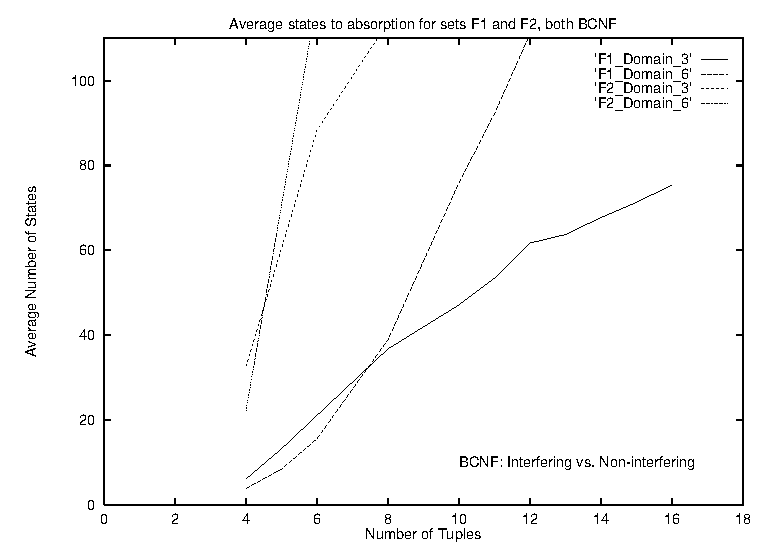
\includegraphics{figures/sets50_82.eps}}}
\caption{\label{graph:16_82}{Average states to absorption for sets $F_1$ and $F_2$, Domain sizes: 3, 6}}
\end{figure}
\index{Similarity Measure}
Most evolved relations for FD sets achieved a quality of 1, using
our similarity measure~\ref{eq:quality}, once the
tuple size was above $\mid$ GEN(F) $\mid + 1$, detailed in \cite{cl96}.
 This is because the probability
of evolving an Armstrong relation is evidently lower when the tuple size
 is below
$\mid$ GEN(F) $\mid + 1$. With a larger domain the chance of an example
relation being Armstrong is significantly lower, especially when the
domain and tuple sizes are comparable, often leading to a trivial
satisfaction of the FDs as well as FDs outside the specified set.
For an empty FD set over $R$ any random relation with schema $R$ satisfies this set;
in terms of quality every possible FD would need to be violated for such
a relation to be Armstrong.
 With a null FD set $\mid$ GEN(F) $\mid = \mid R \mid$ and so
anything larger than a binary domain is unlikely to ever be an Armstrong
relation given the possible spread of all random relations. A measure
of the pathology of an FD set F can be
 provided by the ratio
of the determinations in F to the number of all possible determinations
which can occur over the schema $R$.
Given an attribute set and an FD set
which explicitly specifies all possible non-trivial FDs which
can hold amongst the attributes except for one FD then it is highly likely that
many relations will be evolved which in addition violate this FD. Thus within
such a batch it is likely that many example evolutions will be Armstrong
relations. 

\medskip

The evolutionary procedure is now highlighted with a real world 
example. A greater understanding of the semantics of 
an FD set
is reached by repeated examinations of different instances of the
example relations; this is one motivating factor behind our probabilistic approach.
\index{Evolutionary Algorithm!Example}
\begin{example}
\begin{rm}
We use the following non-BCNF FD set F =
$\{ Name \to Phone$ $Flat No.$, $Flat No. \to Name$, $Postcode \to City \}$.
We present a deterministic Armstrong relation for this set of 
dependencies in Table~\ref{table:5.31} together with two different
evolved Armstrong relations 
of varying tuple and domain size. An evolved
Armstrong relation is shown in Table~\ref{table:5.32} with the same
domain size and tuple number as that used in a deterministic
generation. A quick 
inspection of these two relations shows that the differences in 
Armstrong relations with the same domain and tuple sizes tend to be
superficial, yet the stochastic nature of the generation of relations leads
 a more well-rounded view of the data. Table~\ref{table:5.34} contains another Armstrong relation, 
extending the domain size of the deterministic Armstrong relation
slightly with an attribute domain size of 8 over 9 tuples. In
this instance a larger relation highlights both the satisfied
and violated dependencies, those which are not logically implied by F
such as $Phone \to Name$, thoroughly. 
\end{rm}
\end{example}
{\line
\begin{table}[ht]
\begin{center}
\begin{tabular}{|c|c|c|c|c|} \hline 
{ \bf Name} & { \bf Phone} & {\bf Flat no. }  & { \bf Postcode}  & {\bf City} \\ \hline
Dave & 1246 & 19 & NW1 & London  \\
Dave & 1246 & 19 & YO2 & York \\
Dan & 3748 & 7 & YO2 & York \\
Dan & 3748 & 7 & YO1 & York \\
Charles & 3748 & 11 & YO1 & York \\ \hline
\end{tabular}
\end{center}
\caption{\label{table:5.31} Mannila's deterministic AR}
\end{table}
}
{\line
\begin{table}
\begin{center}
\begin{tabular}{|c|c|c|c|c|} \hline 
{ \bf Name} & { \bf Phone} & {\bf Flat no. }  & { \bf Postcode}  & {\bf City} \\ \hline
Dave & 1246 & 19 & NW1 & London  \\
Dave & 1246 & 19 & YO2 & York \\
Dan & 3748 & 7 & NW1 & London \\
Dan & 3748 & 7 & W14 & London \\
Charles & 1246 & 11 & YO2 & York \\ \hline
\end{tabular}
\end{center}
\caption{\label{table:5.32} An evolved AR with the same domain size }
\end{table}
}

{\line
\begin{table}
\begin{center}
\begin{tabular}{|c|c|c|c|c|} \hline 
{ \bf Name} & { \bf Phone} & {\bf Flat no. }  & { \bf Postcode}  & {\bf City} \\ \hline
Dave & 1246 & 19 & NW1 & London  \\
Dave & 1246 & 19 & W14 & London \\
Dave & 1246 & 19 & YO3 & York \\
Dan & 1246 & 7 & BS8 & Bristol \\
Dan & 1246 & 7 & BA1 & Bath \\
Dan & 1246 & 7 & BA2 & Bath \\
Charles & 1246 & 11 & YO2 & York \\
Matt & 8881 & 84 & BA8 & Bath \\
Fred & 2383 & 24 & YO3 & York \\ \hline
\end{tabular}
\end{center}
\caption{\label{table:5.34} An evolved AR with 9 tuples }
\end{table}
}

\medskip
\index{Pathological Sets}
We briefly introduce pathological sets, these being
the sets for which an Armstrong relation was only rarely,
or in some cases never, achieved are discussed more fully in \cite{cl96}
We remark that these FD sets contain many FDs which determine
few attributes without attributes on their lhs being determined,
remembering that 
our algorithm is not concerned with such relationships.

\medskip
To conclude, the results have shown that example relations which satisfy sets
of FDs can be efficiently evolved. The many different
relations which can be studied for the same FD set also provide a
more well-rounded view of the data in the designer's mind.
Batches containing
many evolutions can be run and a database designer would then be able
to view many relations, including those that are Armstrong if the domain
and tuple sizes satisfy the size bounds and an Armstrong relation
was actually evolved.  If they do not, either domain
or tuple size being too low, then the designer can view an
approximation to an Armstrong which a batch has provided. In
non-pathological cases we conjecture that
this will be the best, or close to the best, approximation to Armstrong
which exists.

\section{Discussion}\label{sec:nd_disc}

In the chapter we have defined a metric for NDs which we will use in
Chapter~\ref{chap:consistency}. We reiterate that the goal of data
mining with NDs is not to determine a proportion of the database in
which a functional relationship is not satisfied but a value for a
numerical satisfaction which approximates functional
satisfaction. Such mining has been shown to be of use with respect to
cardinality constraints in the context of the ER model
\cite{sou98}. Efficient implementations of algorithm~\ref{alg:mine} 
warrant further investigation. Work in \cite{hkp98} which
includes computing partitions as a product of previous partitions within
the lattice of attribute sets as well a pruning the search space if an
FD is found to hold would be directly applicable for ND mining.

\medskip
\index{Database Design}
For design purposes the evolution of example relations has been shown to
be a potentially useful tool.  A good database
design tool is based on ease of use for the designer and example relations
are a step in this direction. To study the applicability of a set of FDs
 the user can limit the number of tuples in
a relation as well as the domain size. The simulations have shown that 
informative example relations can be evolved by our process.  The 
average number of states to evolution is dependent on both
the nature (non-interfering or interfering) and size of the FD set and the size of the relation.
Example relations containing attributes independent of each other
are less likely to be evolved into Armstrong relations. For 63 out
of the 72 sets of FDs used in simulations an Armstrong relation was evolved
for some domain/tuple combination; this is an important side-effect
of our approach and may form the basis for further research.

\medskip

This work
will be of use to the database designer as an auxiliary tool to complement
the other stages of the design process.  From a schema the designer is now
 able to evolve many varied example relations.

\medskip

In the domain of Armstrong relations it would be highly interesting to
study algorithms for the generation of weak Armstrong Relations,
defined in Definition~\ref{def:weak_AR}, in the manner of
\cite{fag82,bdfs84} which examine ARs for FDs in the context of
improving database design.





\chapter{The Consistency Problem in Indefinite
Relations}\label{chap:consistency} 
\index{Consistency Problem}
\index{NP-Complete|see{Consistency Problem}}

In this chapter we demonstrate how NDs may be applied within a
heuristic chase based algorithm for approximating solutions to the
consistency problem \cite{vn95}. We also demonstrate how resampling
may be applied in a dynamic fashion to decide upon suitable sample
sizes for the indefinite relation in question.

\medskip

Our approach to approximating the consistency problem is presented in
Section~\ref{sec:conprob}. In Section~\ref{sec:intro} we motivate the
application of indefinite 
information in relations, referring to the work of
\cite{vn95,inv91,ivv95}.   Section~\ref{sec:algdes} details our
approach to the consistency problem, detailing the chase procedure for
indefinite information relations, the algorithms applied and the use
of two resampling techniques, the bootstrap and the jackknife, for
sample size determination. Section~\ref{sec:cpresults} presents the
extensive simulations conducted on randomly generated indefinite
relations, both uniform and biased with respect to indefinite cell
appearance. We also detail how the simulations were
assessed and the results achieved. We conclude in~\ref{sec:cp_disc}
with a discussion of further work and introduce how our work might be
extended to search for phase transitions using our approximation
technique for relations containing indefinite information.


\section{Our Approach to the Consistency Problem}\label{sec:conprob}
\index{Consistency Problem}


Given a set of FDs F and an indefinite relation $r$ (a relation with one or
more indefinite cells) we tackle the problem of attempting
to find a definite relation extracted from $r$ which satisfies F.
This is widely known as the {\em consistency problem}.  
The consistency
problem has been shown to be NP-Complete in general, and of 
polynomial time complexity in the case where indefinite information is
only allowed in attributes which are present in the right hand side of
FDs (referred to as a {\em good} database) or when the FDs have a
singleton right hand side and attributes with a domain size of
at most arity two are allowed in the left hand side \cite{vn95}. 
 Henceforth, we refer to definite relations as {\em possible worlds}.
An incomplete relation can be seen as a collection of possible worlds
where each world contains a complete instance of the incomplete
relation. 
\index{Consistency Problem!Definition}
\begin{definition}[The consistency problem]\label{def:cons}
\begin{rm}
Given a set of FDs F and an indefinite relation $r$ the {\em consistency problem}
is the problem of deciding whether there exists a possible world in
$r$ which satisfies F, written as $r \weak$ F, see Definition~\ref{def:sat-indef}. $\quad\Box$
\end{rm}
\end{definition}


Our approach in attempting to solve the consistency problem is based on using
a chase procedure, adapted from the standard chase of
Section~\ref{subsec:rev_chase} for indefinite relations, as a
heuristic in conjunction with a hill-climbing 
technique. We start by applying the chase procedure to remove
inconsistent data from the relation which does not satisfy an
initial ND set. For an ND X $\to^k$ Y the chase procedure will
collect $k + 1$ tuples and remove values from indefinite cells
which would otherwise prevent X $\to^k$ Y being satisfied and whose
removal will not prevent the generation of worlds satisfying ND sets
higher in the lattice.
If there is {\em inconsistent} information, implying that 
X $\to^{k+1}$ Y is
the closest ND to an FD which the relation satisfies, then the
chase applied for \linebreak X $\to^k$ Y will return an undefined relation
containing empty cells, indicating that the result of this is {\em undefined}.

\smallskip

The algorithm applies this procedure in a hill-climbing manner
whereby each iteration generates a possible world satisfying an ND set
N from an indefinite
relation $r$. 
After each iteration the chase is applied to $r$ using the best ND set
found so far. This procedure is repeated until 
the chase returns either an undefined result, stating that it can get no
closer to an FD set, or the limit on the number of worlds to
generate is exhausted.  In contrast to this, a naive procedure
was also used which randomly generates $n$ possible worlds and stores
the best approximation. 
For the purposes of this experiment we assume that all possible worlds
are equally probable having a uniform distribution. Changing this assumption,
for instance by assuming an increased weighting of a particular attribute 
domain value, leads to different results, briefly discussed in
Section~\ref{subsec:cp_bias}. 

\smallskip

We wish to know what is a suitable limit on the generation of possible 
worlds to give the hill-climbing
chase procedure. An appropriate size is one which is large enough such
that the probability of obtaining the {\em best possible approximation} to
the FD set is high. Though we may expect such a size to be exponential
in the cardinality of the relation $r$, the schema, and the arity of the indefinite cells,
it would be foolish to generate a figure without examination or
sampling of the data in $r$. Therefore we use the Bootstrap procedure
\cite{et86,et93}, a computationally intensive statistical procedure,
introduced in Chapter~\ref{chap:review}. We
initially take a sample of $n$ observed possible worlds. Based upon this sample
we perform a number of bootstrap replications. Each bootstrap
replication samples from the observed possible worlds with replacement.
In this way the Bootstrap is used to provide a guide to the 
distribution of the possible worlds \cite{dop94}. The key assumption
we make in this 
case is that our sample of observed possible worlds is representative
of the indefinite relation. We then repeat the Bootstrap with an increasing
sample size of observed possible 
worlds. After each bootstrap iteration we calculate the mean and 
standard error.  The number of observed possible worlds (sample size)
 is increased
until the Bootstrap procedure converges to an approximate fixpoint.

In this sense the convergence of the Bootstrap mean value
tells us, with a high probability, that
increasing the sample size further will not provide us with any
additional information concerning the distribution of data within the
indefinite relation. Our 
results have shown this convergence always occurs with a sample size 
that is an upper bound on the 
number actually used by the chase hill-climbing procedure. This is a novel
application of sampling within databases, to our knowledge not
previously used. To illustrate its usage, a relation with 
minimal indefinite information and therefore only
a few possible worlds will have much less variance amongst the satisfaction
of numerical dependency sets. In such a case the bootstrap will reach
a fixpoint after few iterations with a final sample size of $\rho$. The
chase and hill-climbing algorithm will then have $\rho$ as a limit on
the number of worlds to generate and apply heuristics to. This will be
an upper bound based on the minimal variance within the relation.

\smallskip

In order to test the viability of our approach we conducted simulations
over 12 sets of FDs, demarcated into {\em Boyce-Codd Normal
Form}(BCNF), see Definition~\ref{def:bcnf}, 
and non-BCNF, ranging from small to large sizes. 
 Each FD set was evaluated with respect to the average and maximum number
of worlds generated and the final value of the {\em best} ND set.
This was performed for around 100 batches, each containing 500 runs, a
single run being the process of applying the 
chase and hill-climbing process until we can climb no further. 
Each batch was varied over domain, tuple
and maximum cell arity size each held constant within a
particular batch. The batches were all repeated for the naive procedures. The
parameters 
were varied from a range of trivial satisfaction to trivial inconsistency
within a relation. Across batches the weighting of the number of 
indefinite cells appearing in a relation was also varied from a 25\%
to a 75\% likelihood with this weighting given to cells which are
in an attribute present in the left hand side of an FD or not.
The simulations
emphasised the validity of the chase hill-climbing procedure noting that
far fewer worlds are used (before any further chase iterations create
an undefined relation) to provide a similar result to the generation of
a very large number of possible worlds, the naive
approach. Additionally, the run times for the chase and hill-climbing
algorithm were much faster than the corresponding naive algorithm. The higher
the degree of indefinite cells in a relation tended to provide better
results when using the chase hill-climbing approach.
 The simulations also showed that our
use of the Bootstrap for parameter setting is both valid and useful.
Indeed, the application of such statistics seems set to become more
commonplace in data mining, as was recently expressed by U. Fayyad in
a data mining journal, ``I personally look forward to the
proper balance that
will emerge from the mixing of computational algorithm-oriented
approaches characterizing the database ... with the powerful
mathematical theories and methods for estimation developed in statistics''
\cite{fay98}.

\cite{inv91} motivated the use of indefinite information within a 
relation using a scheduling application and in this context the consistency problem is equivalent to
asking whether a particular schedule in invalid. \cite{vn95} presents
a relationship between work on indefinite information and {\em constraint
logic programming}. \cite{vhe89} presents a number of logic programs
which incorporate domain constraints and use them to aid solving
various programs, ranging from simple puzzles to search
algorithms. Our methodology could be applied to instances of such
puzzles in cases where approximations to a final answer are satisfactory.

\subsection{Intractability of the consistency problem}
\index{Consistency Problem!Intractability of}
It was shown in \cite{vn95} that the consistency problem is,
in general, NP-complete \cite{gj79}.  It follows that the 
corresponding consistency problem for NDs is also
NP-complete, since FDs are a special case of NDs.
In the special case when for all attributes A in the left-hand sides 
of the FDs in F the A-values of all the tuples in $r$ are definite,
then the consistency problem can be solved in polynomial time
in the sizes of F and $r$ \cite{vn95}.
The NP-complete nature of the consistency problem inherently
implies that it would be fruitless to design an algorithm which
searches for an exact solution for a relation and a set of FDs. Therefore
our algorithm attempts to find an approximation to the best
solution that is available.

\cite{ivv95} shows how query complexity across more
than a single relation becomes
co-NP-complete when the relations contain indefinite information. Also 
introduced are {\em typing functions}, which state whether an
attribute can contain indefinite information or not and {\em degree of 
co-referencing}, which places restrictions on
the type of indefinite information allowed in a relation. This ranges
from no repetition of OR-objects, no repetition across columns, and
unrestricted repetition. Due to our allowance of indefinite
information directly within cells we inherently allow unrestricted
repetition. \cite{ivv95} identifies a complete characterisation of
queries for the different classes of database, based on the degree of
co-referencing, which are evaluable in polynomial time. This is
intended to provide an outline of the allowed use of queries and
indefinacy within a database so that query complexity remains
within polynomial time.

\medskip

The notion of {\em mutable} and {\em persistent} object identifiers is
also introduced in \cite{inv91}. A {\em persistent} object identifier is where the cell
containing indefinite information is taken as an object which contains a
disjunction (i.e. a name for the object whose value is not yet known)
 whereas in a {\em mutable} object identifier the indefinite
information is interpreted as disjunction across tuples, which
is therefore assumed to have a {\em place-holder} representation.
Mutability is required for structure sharing within indefinite data.
We do not consider this in the context of our work. Mutable object
identifiers generalise marked nulls. 


\section{Indefinite Information in Relations}\label{sec:intro}

In Section~\ref{subsec:rev_indef} we introduced the background on
indefinite information representation in relations principally
focusing on the use of OR-objects. We now discuss applications of
indefinite information and formalise dependency satisfaction.

\subsection{Applications}
\index{Incomplete Information in Relations}
\index{Incomplete Information}
\index{Indefinite Information}
\index{OR-object}
\index{NULL value}
		
Indefinite information representation in relations has been shown to be 
a useful facility for incomplete specifications in design and planning
applications \cite{inv91,ivv95,vn95}. We define {\em indefinite cells} as cells
containing one or more values which represent a set of possibilities denoting
 the current limit of knowledge in the database. Any indefinite cell in 
column A which contains the complete domain allowed for A is equivalent to
the traditional NULL value \cite{lip79}.
 A definite relation extracted from
one containing indefinite information is a relation with the same schema
and definite cells, which are invariant throughout, but with each indefinite
cell, say I, replaced with a definite cell containing one value from I.  
Associated with an indefinite
relation may be a set of integrity constraints, primarily FDs, the
most common integrity constraint in relational databases. 
\medskip


\cite{inv91} introduced OR-objects for use within design, planning and
scheduling operations, motivated by the lack of functionality in
information systems to handle
\begin{itemize}
\item coexistence of objects in different stages within the design
process
\item the ability to evaluate hypothetical queries
\item allowing choice within the data model
\end{itemize}

\cite{inv91} presents differences between the {\em interpretational} and
{\em structural} levels of a schedule. The interpretational level refers to
the final designs, possible worlds in our interpretation, of an
indefinite relation whilst at the structural level we are concerned with
the indefinite relation itself. In this work we provide a methodology
for assessing interpretational information content of indefinite
relations. Structural queries discussed in
\cite{iv89,inv91} such as ``are there two people in a travel relation $c$
with common destinations,'' may be addressed by including NDs as
constraints within the respective data model.  \cite{inv91} formalises
views which allow for querying at either the interpretational or
structural level, or a combination of the two. The data complexity of
the query language is shown to be co-NP-complete, correlating with the
proof given in \cite{vn95} that the consistency problem is NP-complete
due to the fact that a query might ask if all schedules are invalid (a
structural query), consistent with all schedules violating an FD set.

\medskip

We now define FD and ND satisfaction in indefinite relations:
\index{Functional Dependency!Satisfaction in an indefinite relation}
\begin{definition}[Satisfaction of an FD in an Indefinite Relation]\label{def:sat-indef}
\begin{rm}
Let $s \in$ POSS($r$), be a definite relation over R.
An FD X $\to$ Y is {\em satisfied} in $s$,
denoted by $s \models$ X $\to$ Y, whenever
$\forall t_1, t_2 \in$ s, if $t_1$[X] = $t_2$[X] then $t_1$[Y] = $t_2$[Y].
A set of FDs F is {\em satisfied} in $s$,
denoted by $s \models$ F, whenever
$\forall$ X $\to$ Y $\in$ F, $s \models$ X $\to$ Y.

\smallskip
\index{Functional Dependency!Weak Satisfaction}
A set of FDs F is {\em weakly} satisfied  
(or simply satisfied whenever no ambiguity arises) in a relation $r$,
denoted by $r \weak$ F, whenever 
$\exists s \in$ POSS($r$) such that $s \models$ F.
If $r \weak$ F we say that $r$ is {\em consistent} with respect to F 
(or simply $r$ is consistent if F is understood from context);
otherwise if $r \notweak$ F then we say that $r$ is {\em inconsistent}
with respect to F (or simply $r$ is inconsistent).$\quad\Box$
\end{rm}
\end{definition}

As for standard relations in Section~\ref{subsec:rev_ndtheory}, we
generalise the concept of an FD by an ND. 
 

\index{Numerical Dependency!Satisfaction in an indefinite relation}
\begin{definition}[Satisfaction of an ND in an Indefinite Relation]\label{def:sat-nd-indef}
\begin{rm}
Let $s \in$ POSS($r$), be a definite relation over R.
An ND X $\to^k$ Y is {\em satisfied} in $s$,
denoted by $s \models$ X $\to^k$ Y, whenever
$\forall t_1, t_2, \ldots, t_k, t_{k+1} \in$ s, if 
$t_1$[X] = $t_2$[X] = $\ldots$ = $t_k$[X] = $t_{k+1}$[X] then 
$\exists i,j$ such that $1 \le i < j \le k+1$
and $t_i$[Y] = $t_j$[Y].
A set of NDs N is {\em satisfied} in $s$,
denoted by $s \models$ N, whenever
$\forall$ X $\to^k$ Y $\in$ N, $s \models$ X $\to^k$ Y.

\index{Numerical Dependency!Weak Satisfaction}
We define a set of NDs N to be weakly satisfied in a relation $r$
in the same way as for FDs; similarly we define 
a relation $r$ to be consistent with respect to a set of NDs if
$r \weak$ N and otherwise to be inconsistent.$\quad\Box$
\end{rm}
\end{definition}

\smallskip

The use of NDs in possible worlds to approximate FD set satisfaction
in an indefinite relation has not previously been considered to our
knowledge. 

\section{Algorithm design}\label{sec:algdes}
\index{Bootstrap Resampling}
\index{Jackknife Resampling}

We now present an overview of the component parts of our process for
approximating solutions to the consistency problem. We begin with a
presentation of the chase for NDs in indefinite relations, followed by
an overview of our use of resampling.  The principal algorithms are
then introduced.

\subsection{The chase algorithm for indefinite
relations}\label{subsec:cp_ndchase}
\index{Chase Procedure!for NDs in Indefinite Relations}

In Algorithm~\ref{alg:cp_ndchase}, ND\_CHASE, we present the chase for
NDs in indefinite relations,  
called within CHECK\_CONS. It is a heuristic procedure extended from the
standard chase procedure for FDs \cite{bv84,Mann92} which, given a set
of NDs, attempts to remove extraneous or redundant information that 
may otherwise prevent the ND set from being satisfied. The forward chase
removes extraneous values 
from indefinite cells in attributes which are in the right hand
side of a given FD which is satisfied numerically but not functionally and 
therefore generalised to an ND.  Informally, a partition on attributes
in the left
hand side of the FD which has at least one more tuple than the
branching factor of the
ND is selected 
and indefinite cell values of attributes in the right hand side of the
FDs, whose appearance in a possible world would cause the ND to
be unsatisfied, are removed. The backward chase removes values from
indefinite cells in attributes on the left hand side of the given
FDs which would have otherwise prevented satisfaction of the current
ND if that value had been selected for inclusion within a possible world.



{\line
\begin{figure}[ht]
\fbox{\begin{minipage}{14cm}
\begin{algorithm}[{\rm ND\_CHASE}($r$, {\rm N})]\label{alg:cp_ndchase}
\begin{rm}
\begin{tabbing}
t1\=t2\=t3\=t4\=t5\=t6\=t7\= \kill \\
1.  \> \> {\bf begin} \\
2.  \> \> \> Result := $r$; \\
3.  \> \> \> Tmp := $\emptyset$; \\
4.  \> \> \> {\bf while} Tmp $\not=$ Result {\bf do} \\
5.  \> \> \> \> Tmp := Result; \\
6.  \> \> \> \> {\bf if} $\exists$ X $\to^k$ Y $\in$ N, $\exists t_1, t_2, \ldots, t_k, t_{k+1} \in$ Result such that  \\
    \> \> \> \> \> $t_1$[X], $t_2$[X] $\ldots$, $t_k$[X], $t_{k+1}$[X] are definite and $t_1$[X] = $t_2$[X] = $\ldots$ = $t_k$[X] = $t_{k+1}$[X] \\
    \> \> \> \> \> but $t_1$[Y] $\not=$ $t_2$[Y] $\not= \ldots \not=$ $t_k$[Y] $\not=$ $t_{k+1}$[Y] {\bf then} \\ 
7. \> \> \> \> \> {\bf for each} $A \in$ Y$-$X and $v \in t_{k+1}$[A] {\bf do} \\
8. \> \> \> \> \> \> {\bf if} $v \not\in \bigcup_{i=1}^k t_k$[A] and $\forall i,j \in \{1,2,\ldots,k\}$ such that $i \not= j$, $t_i$[A] $\cap t_j$[A] = $\emptyset$ {\bf then} \\
9. \> \> \> \> \> \> \> $t_{k+1}$[A] := $t_{k+1}$[A] $- \{v\}$; \\
10. \> \> \> \> \> \> {\bf end if} \\
11. \> \> \> \> \> {\bf end for} \\
12.  \> \> \> \> {\bf end if} \\
13. \> \> \> \> {\bf if} $\exists$ X $\to^k$ Y $\in$ N, 
$\exists t_1, t_2, \ldots, t_k, t_{k+1} \in$ Result such that  \\
    \> \> \> \> \> $t_1$[XY], $t_2$[XY], $\ldots$, $t_k$[XY], $t_{k+1}$[Y$-$X] are definite and $t_1$[X] = $t_2$[X] = $\ldots$ = $t_k$[X] \\
    \> \> \> \> \> and $t_1$[Y$-$X] $\not=$ $t_2$[Y$-$X] $\not= \ldots
\not=$ $t_k$[Y$-$X] $\not=$ $t_{k+1}$[Y$-$X] and  \\
    \> \> \> \> \> sound($t_1$[X],$t_2$[X],$\ldots$,$t_k$[X],$t_{k+1}$[X]) {\bf then} \\ 
14. \> \> \> \> \>  $\forall$ A $\in$ X$-$Y,  $t_{k+1}$[A] := $t_{k+1}$[A] $-$ $t_i$[A], for some $i \in \{1,2,\ldots,k\}$; \\
15. \> \> \> \> {\bf end if}\\
16.  \> \> \> {\bf end while} \\
17. \> \> \> {\bf return} Result;  \\
18. \> \> {\bf end.}
\end{tabbing}
\end{rm}
\end{algorithm}
\end{minipage}}
\caption{\label{cp:fig:indef_chase} Chase for Numerical Dependencies with forwards and backwards tests}
\end{figure}
}

We include the {\em sound} check for the attributes values on the left
hand side of an ND \linebreak X $\to^k$ Y to ensure that values are not removed
unnecessarily 
from cells which might otherwise form an attribute value combination over X
which is not present in any of the tuples in $\{$ $t_1$[X], $t_2$[X],
$\ldots$, $t_k$[X] $\}$ and therefore not redundant. If this step were
not performed we might 
create an undefined relation unnecessarily. To illustrate this we
present Table~\ref{tbl:backchase1} showing an indefinite relation over
ABC with an FD AB $\to$ C. If we apply the backwards chase to this
relation without the {\em sound} check then, due to each tuple
disagreeing on C with the indefinite tuple, this would result in an undefined
relation. Table~\ref{tbl:backchase2} depicts the satisfying instance.

{\line
\begin{table}[ht]
\begin{minipage}[b]{7cm}
\begin{center}
\begin{tabular}{|c|c|c|} \hline
 {\bf A} & {\bf B} & {\bf C} \\\hline
 0 & 0 & 0 \\ 
 0 & 1 & 0 \\ 
 1 & 0 & 0 \\ 
 $\{$0,1$\}$ & $\{$0,1$\}$ & 1 \\ \hline
\end{tabular}
\end{center}
\caption{\label{tbl:backchase1}Indefinite relation $r$, FD AB $\to$ C} 
\end{minipage}
\hfill
\begin{minipage}[b]{7cm}
\begin{center}
\begin{tabular}{|c|c|c|} \hline
 {\bf A} & {\bf B} & {\bf C} \\\hline
 0 & 0 & 0 \\ 
 0 & 1 & 0 \\ 
 1 & 0 & 0 \\ 
 1 & 1 & 1 \\ \hline
\end{tabular}
\end{center}
\caption{\label{tbl:backchase2}A satisfying world for AB $\to$ C} 
\end{minipage}
\end{table}
}

\begin{definition}[Good Classes of Indefinite relations, \cite{vn95}]\label{cp:def_good}
\begin{rm}
Given a relation $r$ and a set of FDs F,
$r$ is { \em good} for F if it contains no indefinite cells in $r$ on any
of the attributes which are also on the left hand side of any FD in
F. $\quad\Box$ 
\end{rm}
\end{definition}
\smallskip
An $O(n^2)$ algorithm, DELETE\_REDUNDANT, is presented in \cite{vn95} that takes a relation good for F, and
pre-processes it such that the resulting relation has only conforming
possible worlds.  It is said to {\em fully incorporate} any set of FDs in
a database $D$ if the database is good for the set of FDs; it is
equivalent to ND\_CHASE with 
only a forward chase component. The algorithm maintains a cumulative
domain of all the OR-objects; the relation $r$ is partitioned for
agreement on the attributes in the body of F and each partition
has an intersected domain of all OR-objects within the attributes
on the right hand side of F. It is shown to be
sound given that \cite{vn95} accept, without comment, that a
relation that is not satisfying will have a null-intersection on its
OR-objects and will not therefore have any possible worlds.\\


\subsection{Resampling for the Consistency Problem}
\index{Resampling!for consistency problem}
Given that the number of  possible worlds of an indefinite relation increases
exponentially in the size of the relation  it is impossible to
examine all possible worlds for the best solution.  The
complete population distribution is unknown; otherwise we would know 
exactly how many definite relations to
generate to have a specific probability of finding the closest ND set
to the given FD set.  This suggests 
applying a bootstrap procedure to a sample of definite instances 
to approximate the population distribution based on the sample
distribution.  Essentially we take a sample of
$n$ possible
worlds from an indefinite relation. Then we use the sample
to construct pseudosamples of size $n$, obtained by selecting
randomly from the sample with replacement for each pseudosample. 
We then increase the sample size by a small amount $\delta$ and repeat
the bootstrap procedure with sample size $n + \delta$ until a fixpoint
is reached and subsequent increases do not affect the variance any further.
Informally, we use this incremental
bootstrap procedure to tell us how many worlds we need 
to consider so that we have a high confidence that generating additional
worlds will not improve our solution.

\medskip

Independently of this work we refer the reader to \cite{jl96} which
defines dynamic sampling as, ``the use of knowledge about the
behaviour of the mining algorithm in order to choose a sample size.''
Within the context of this work, we prefer to define dynamic sampling
as the use of knowledge about the data to choose a sample size. Our
incorporation of resampling does exactly this.
\cite{jl96} note that in data mining and decision support it is
important that the sample size is well chosen.  Indeed, a poorly
chosen sample size which may not accurately capture the information
content of a database to within the correct degree of error, may
result in a loss of much money. \cite{jl96} therefore introduces the
PCE (Probably Close Enough) inequality, a derivation of the
PAC-learning criterion \cite{val84,ab92}, which states that
\[
Pr(acc(D) - acc(s) > \epsilon) \le \delta
\]
where acc measures the accuracy of the mining algorithm, $D$ refers to
the database, $s$ the sample and $\epsilon$ and $\delta$ are error and
confidence limits, respectively. \cite{jl96} assumes that whenever
$acc(s_{i+1}) \le acc(s_i)$ 
then further increases in sample size will result in a loss of
accuracy and that $n_i$ is a suitable sample size, given that the
derivative of accuracy with respect to sample size has become
non-positive. \cite{jl96} state 
that it is necessary to estimate $acc(s_i)$ and uses leave-one-out
cross-validation to achieve this; we choose instead to use bootstrap resampling for
our estimation of a sample size. 
Similarly, our
employment of dynamic resampling assumes that when we reach an
approximate fixpoint no further increases in sample size will improve
the knowledge of the indefinite relation. 

\subsection{The Bootstrap Process within Indefinite Relations}\label{subsec:boot_proc}
\index{Resampling!Bootstrap}

The bootstrap is a data driven simulation method for
statistical inference. It is a computationally intensive procedure
that has been shown to ably provide confidence limits which would not have
been capable of being similarly generated more than 30 years ago.
In our experience, statistical methods have not previously been 
applied in the solution of database problems such as the consistency problem.
We now formalise the use of the bootstrap in indefinite relations.
\medskip

\begin{figure}[ht]
\centerline{\scalebox{0.7}{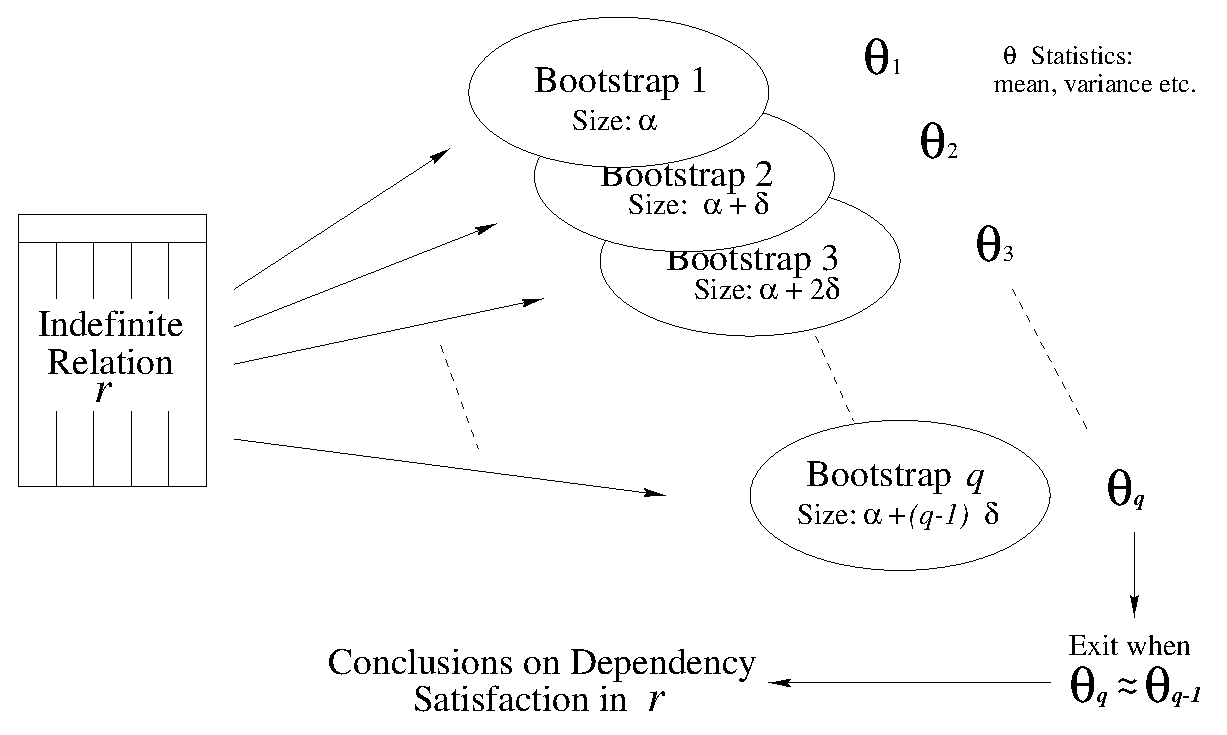
\includegraphics{consistency/dyn_bootstrap.eps}}}
\caption{\label{fig:inc_boot} The Bootstrap procedure applied to
increasing sample sizes for an indefinite relation}
\end{figure}
\index{Bootstrap!Sample of indefinite relations}
\begin{definition}[The Bootstrap Sample]
\begin{rm}
Given an indefinite relation $r$ over schema $R$ where $\mid R \mid$ =
$m$ and $\mid r \mid$ = $v$ and the maximum arity in an
indefinite cell is $q$, then $r$ can have {\em at most} $q^{mv}$ possible
worlds.  From $r$ we uniformly randomly extract $n$ possible worlds.
Each of these worlds will satisfy a set of NDs (which may be FDs). These $n$ possible
worlds are referred to as the original sample or {\em observed possible 
worlds }
and are written as {\bf $\tilde{p}$} = $(r_1, r_2, \ldots, r_n)$. A
bootstrap sample is {\bf $\tilde{p}^\star$} = $(r_1^\star, r_2^\star, \ldots, r_n^\star )$ where for all $i = 1,2 \ldots, n$ each $r_i^\star$ is randomly
selected with replacement from the $n$ observed possible worlds,
{\bf $\tilde{p}$}.$\quad\Box$
\end{rm}
\end{definition}

The probability of an observed possible world {\em not} being
present in a bootstrap sample of size $n$ is $(1 - \frac{1}{n})^n$
assuming each world in the sample has a $\frac{1}{n}$ chance of being
selected.  Note that
every observed possible world has an equal likelihood of being 
selected for each point in the Bootstrap sample. The ND set is
restricted to expressing approximations to a given FD set in this work.

\medskip

We denote each of the $l$ NDs which may hold in
$r$ by $X_i \to^{k_i} Y_i$ where $1 \le i \le l$.
We denote the branching factor $k$ which holds for ND $X_i \to^k Y_i$ in
$r$ as $br_{X_iY_i}$($r$).  
\index{Bootstrap!Sample mean}
\begin{definition}[The Bootstrap Sample Mean]
\begin{rm}
Given a bootstrap sample {\bf $\tilde{p}^\star$} = \linebreak[4] $(r_1^\star, r_2^\star, \ldots, r_n^\star )$, we calculate the
mean $\bar{s}(\cdot)$, or any other statistic of interest, in exactly the same
way as we would have for the original sample of ND sets, each containing $m$ NDs, 
\[\bar{s}(\tilde{p}^\star) = \{ X_j \to^K Y_j \mid 1 \le j \le m \}\quad\mbox{ where}\quad K = {\Sigma_{i = 1}^n br_{X_jY_j}(r_i^\star)/n}\]
When we refer to the sample mean of a set of possible worlds we are implying
the sample mean of the sets of NDs of the possible worlds.$\quad\Box$
\end{rm}
\end{definition}


\index{Bootstrap!Replication Size}
\begin{definition}[The Bootstrap Replication Size (BRS)]
\begin{rm}
The Bootstrap Replication Size, $B$, is the number of times a Bootstrap
sample of size $n$ is created from the observed possible worlds (the
original sample) and evaluated on a parameter of interest. We denote the $B$ bootstrap samples by $\tilde{p}^\star_b$ = ({\bf $\tilde{p}^\star_1, \tilde{p}^\star_2, \ldots, \tilde{p}^\star_B$}).$\quad\Box$
\end{rm}
\end{definition}

\index{Bootstrap!Mean of all values}
\begin{definition}[The Bootstrap Mean of all Values]
\begin{rm}
Given a set of $B$ bootstrap samples $\tilde{p}^\star_b$,  
we calculate the mean $\bar{s}(\cdot)$, or any other statistic of 
interest, in exactly the same
way as we would have for the original sample, 
$\bar{s}(\tilde{p}^\star_b)$  = $\Sigma_{i = 1}^B \bar{s}(\tilde{p}^\star_i) / B$.$\quad\Box$
\end{rm}
\end{definition}


\cite{et93} tackles how large the BRS should be. Given a BRS $B$, \cite{et93}
refers to the {\em ideal bootstrap estimate} which takes $B$ equal to
infinity. As $B$ increases the empirical standard error tends towards
the standard error of the original sample. Therefore the population
distribution of
the resamples are based on the population distribution found in the
sample; this emphasises the {\em non-parametric} nature of the bootstrap.
\cite{et93} show that the amount of computation time required for increasing
BRS sizes grows linearly. We show that this is also the case for 
increasing the BRS for indefinite relations in Figure~\ref{graph:linboot}
where new FDs, determining a new attribute, are added.
Figure~\ref{graph:linboot} represents a near {\em worst case scenario}
where each FD added to the 
set determines a single attribute where all of its cells are indefinite, of
arity 3, and intersect on only one value. The number of tuples in the
relation and both the degree of indefinite cells and arity of these
cells affects the gradient of these lines.


\begin{figure}
\centerline{\scalebox{0.7}{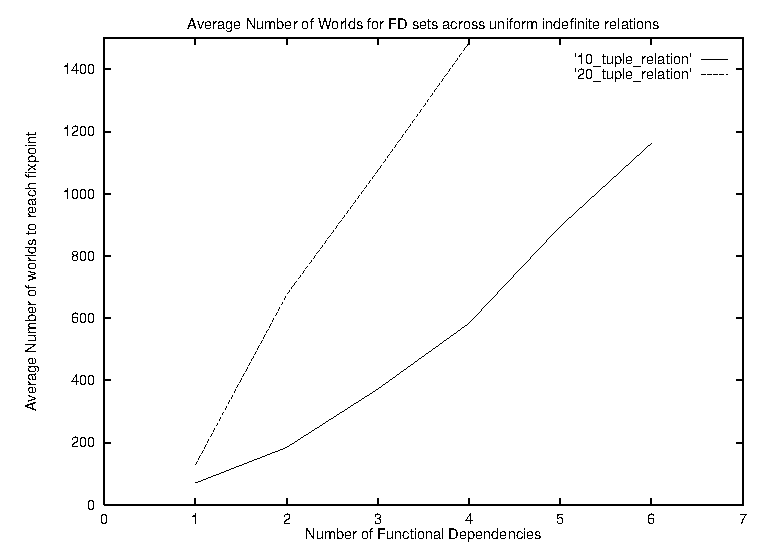
\includegraphics{figures/boot_mean1.eps}}}
\caption{\label{graph:linboot} {Average number of worlds to
reach an approximate fixpoint of the mean bootstrapped ND values in 10
and 20 tuple random relations}}
\end{figure}

\index{Bootstrap!Standard Error}
\begin{definition}[The Bootstrap Standard Error for Indefinite Relations]
\begin{rm}
The sample standard error in the values for $B$ bootstrapped
values is:
\begin{displaymath}
\hat{se}_B(\tilde{p}^\star_b) = \{ \frac{1}{B}\Sigma_{i = 1}^{B}(\bar{s}(\tilde{p}^\star_i) - \bar{s}(\tilde{p}^\star_b)) \}^{1/2}\quad\quad\Box
\end{displaymath}
\end{rm}
\end{definition}

We now describe the methods of our Bootstrap application, detailed in
Algorithm~\ref{alg:blimit}. The process is outlined in
Figure~\ref{fig:inc_boot}.
We start with a small initial sample size $\alpha$ and a 
Bootstrap Replication Size $B$. 
Having created $B$ bootstrap samples we will have a bootstrap
mean of all values in the form of an ND set. For this value
we can use the bootstrap to calculate the standard deviation
(and other statistics if desired). From this we can empirically infer
the width of the interval 
in which a certain percentage of the relations occur. We continue
to increase $\alpha$ by a fixed amount, $\delta$, until we reach 
a point where
the mean value of the NDs in the ND set converge. In
Figure~\ref{fig:inc_boot} this occurs after $q$ bootstrap applications
on different sample sizes. This 
provides a parameter whereupon any samples larger than $\alpha + (q-1)
\delta$ is unlikely to have 
any significant change in variance. It is unlikely, even for an ND set with
just one dependency, for this to be reached randomly and running
our simulations in batches of 500 implied that any erroneous fixpoint
values as outliers would have a negligible impact on the final results.

\medskip

We also examined the variance of the
observed possible worlds, for a range of original sample sizes,
 as the bootstrap replication
size was scaled from 20 up to 50,000 to decide on a suitable BRS,
detailed more fully in Appendix~\ref{app:sim_meth}.
As this was increased we noted that
above 1000 there was negligible change in the variance. Extensive research
on the bootstrap has shown that even for BRS of 25 useful inferences
can be made, and that there is seldom a significant change once a BRS
is over 200 \cite{et86}.
For the purposes
of our experiment setting $B$ at 100 gave a suitable value
which allowed sufficient repetitions of the complete bootstrapping process
in a reasonable time, knowing that there would be only a minimal change
in the variance for any increase in $B$. Additionally we experimented with 
using the original indefinite 
relation for each resampling iteration from which $n$ possible worlds are
sampled each time. The variance is much higher in this case as we
have all possible worlds to select from for each sample of size $n$.
In terms of reaching a fixpoint this takes much longer and was not used
in the final simulations. It could be of use
in situations where the
bootstrap sample may be unrepresentative of the population.


\subsection{Resampling Algorithms}\label{sec:cp_resalg}
\index{Resampling!Bootstrap}
\index{Resampling!Jackknife}

We now formalise the bootstrap and jackknife algorithms used for
resampling and the dynamic algorithm within which they were used for
indefinite relations.
Algorithm~\ref{alg:bstrap}, BOOTSTRAP($N_{bag}$,$s$,$B$),
describes the standard bootstrap procedure which returns the mean value
of ND sets for a BRS value $B$ of Bootstrap replications, sample size $s$ and a
sample population $N_{bag}$ of ND sets. The value $\alpha$
provided by the bootstrap is used both in ND\_GEN and CHASE\_GEN.
Algorithm~\ref{alg:jack}, JACKKNIFE($N_{bag}$), creates $n$ resamples
from $N_{bag}$ where $\mid N_{bag} \mid = n$ and each resample is of
size $n - 1$. This was initially developed before the bootstrap, to
which it has been shown to be an approximation \cite{et86}. It is of
most use when a sample is likely to contain significant outliers. We
discuss its use in Section~\ref{subsec:cp_jackcomparison}. 


{\line
\begin{figure}[ht]
\begin{center}
\fbox{\begin{minipage}[t]{16cm}
\begin{algorithm}[{\rm BOOTSTRAP}($nd\_bag$, $n$, $B$)]\label{alg:bstrap}
\begin{rm}
\begin{tabbing}
t1\=t2\=t3\=t4\=t5\=t6\=t7\=t8\=t9\=t10\= \kill \\
\ra. \>  {\bf begin} \\
\sa. \>  \>  ND\_mean := $\emptyset$ ;\\
\sa. \>  \> {\bf for }  1 to $B$ {\bf do }\\
\sa. \>  \> \> ND\_samp := Uniform Randomly select $n$ ND \\
\> \> \> \> \> \> \> \> sets from $nd\_bag$ with replacement; \\
\sa. \>  \> \> Insert the mean of ND\_samp into ND\_mean; \\
\sa. \>  \>  {\bf end for}\\
\sa. \>  \> {\bf return} the mean of ND\_mean; \\
\sa. \>  {\bf end.}
\end{tabbing}
\end{rm}
\end{algorithm}
\end{minipage}}
\caption{\label{cp:fig:bootstrap} The Bootstrap procedure for
indefinite relations}
\end{center}
\end{figure}
}


{\line
\begin{figure}[ht]
\begin{center}
\fbox{
\begin{minipage}[t]{16cm}
\begin{algorithm}[{\rm JACKKNIFE}($nd\_bag$)]\label{alg:jack}
\begin{rm}
\begin{tabbing}
t1\=t2\=t3\=t4\=t5\=t6\=t7\= \kill \\
\ra. \>  {\bf begin} \\
\sa. \>  \>  ND\_m := $\emptyset$;\\
\sa. \>  \>  $n$ := $\mid nd\_bag \mid$;\\
\sa. \>  \> {\bf for } $j$ := 1 to $n$ {\bf do }\\
\sa. \>  \> \> ND\_samp := $nd\_bag$ - $nd_j$; \\
\sa. \>  \> \> Insert the mean of ND\_samp into ND\_m; \\
\sa. \>  \>  {\bf end for}\\
\sa. \>  \> {\bf return} the mean of ND\_m; \\
\sa. \>  {\bf end.}
\end{tabbing}
\end{rm}
\end{algorithm}
\end{minipage}}
\caption{\label{cp:fig:jackknife} The Jackknife procedure for
indefinite relations}
\end{center}
\end{figure}
}


\medskip
\index{Resampling!Incremental}
\index{WORLD\_LIMIT}
Algorithm~\ref{alg:blimit}, WORLD\_LIMIT($r$, F, $B$), implements our
novel use of the Bootstrap procedure. The initial sample size we
incorporated in our simulations was 10 possible worlds, sufficiently
small for application to all indefinite relations. This could possibly
be extended to using the degree of indefinite cells and the domain sizes
to calculate a suitable initial sample size.
We motivate our procedure on the assumption that different sample sizes are
required according to the variance within an indefinite relation in
the different ND sets which may be satisfied in possible
worlds. The number of dependencies in the given FD set also influences
the results obtained from our use of the bootstrap. In Section~\ref{sol:res}
we show that this application of the bootstrap returns an upper bound on 
the number of worlds required for a good answer. Unlike many statistical
operations, the BOOTSTRAP
algorithm operates in exactly the same manner as a standard bootstrap
procedure despite the fact that we potentially have all possible worlds
within the indefinite relation, unlike many statistical applications
from which inferences are made on incomplete populations.  Based on
this we conducted experiments 
whereby the bootstrap resamples were obtained not from the original
sample but from the indefinite relation. As stated, the variance of resampling
from the relation
was much higher than resampling from the sample and in such cases the
upper bound was much higher. 
Therefore we have found it to be suitable to use just one original sample
from the indefinite relation within each iteration of
WORLD\_LIMIT. This is elaborated upon in Appendix~\ref{app:sim_meth}.

{\line
\begin{figure}[ht]
\begin{center}
\fbox{
\begin{minipage}[t]{10cm}
\begin{algorithm}[{\rm WORLD\_LIMIT }($r$, {\rm F}, {\rm B})]\label{alg:blimit}
\begin{rm}
\begin{tabbing}
t1\=t2\=t3\=t4\=t5\=t6\=t7\= \kill \\
\ra.  \> \> {\bf begin} \\
\sa. \> \> \> $n$ := initial($r$); \% sample size, based on r \\
\sa. \> \> \> ND\_bag := $n$ ND sets from $n$ possible worlds,
each approximating F \\
\sa. \> \> \> $\hat{N}_0$ := $\emptyset$; \\
\sa. \> \> \> $\hat{N}_1$ := BOOTSTRAP(ND\_bag, $n$, B); \\
\sa. \> \> \> $j$ := 1; \\
\sa. \> \> \> {\bf while} $\hat{N}_j,\hat{N}_{j-1}$ are not approx. fixpoint  {\bf do}  \\
\sa. \> \> \> \> ND\_bag := $n$ ND sets from $n$ possible worlds; \\
\sa. \> \> \> \> $\hat{N}_j$ := BOOTSTRAP(ND\_bag, $n$, B); \\
\sa. \> \> \> \> $n$ := $n + \delta$;  \% Increase the sample size by $\delta$ \\
\sa. \> \> \> \> $j$ := $j$ + 1;\\
\sa.   \> \> \>{\bf end while}\\
\sa. \> \> \> {\bf return} $n$;\\
\sa. \> \> {\bf end.}
\end{tabbing}
\end{rm}
\end{algorithm}
\end{minipage}}
\caption{\label{cp:fig:world_limit} The WORLD\_LIMIT algorithm for
incremental bootstrap sampling in indefinite relations}
\end{center}
\end{figure}
}


\subsection{Finding an approximate solution to the consistency problem}
\label{sec:cp_approx}
\index{Consistency Problem!Approximate Solution}
We focus on finding an approximation N of an FD set F for an
indefinite relation \linebreak $r$ such that $r \weak$ N 
using Algorithm~\ref{alg:check}, denoted by CHECK\_CONS($r$, F, $B$),
where $B$ is the bootstrap replication size (BRS).
Recall that we have assumed that $\mid r \mid = m+1$, where $m \ge 1$;
if $\mid r \mid < 2$, then $r \weak$ F trivially holds; 
we refer the reader to Definition~\ref{def:sat-nd-indef}.

We now briefly describe the {\em naive} version of CHECK\_CONS applied
to an indefinite relation and an FD set F. This simply
generates a fixed number of possible worlds, each satisfying an ND set
approximation of F, and returns the ND set with
the closest proximity to that of F. We apply ND\_CHASE
before the generation to remove redundancy, even from the naive selection.
It is quite feasible to consider the use of the bootstrap in conjunction
with a naive approach though this would always generate exactly  
$\alpha$ definite worlds, exactly the figure returned by
WORLD\_LIMIT. 
Use of resampling in a naive procedure is unwarranted given that such
computation time would be better spent generating new possible worlds and not
resampling, which may generate possible worlds that satisfy close
approximations but are not then detected again by a naive procedure.


{\line
\begin{figure}[ht]
\begin{center}
\fbox{\begin{minipage}{16cm}
\begin{algorithm}[{\rm CHECK\_CONS}($r$, {\rm F}, $B$)]\label{alg:check}
\begin{rm}
\begin{tabbing}
t1\=t2\=t3\=t4\=t5\=t6\=t7\= \kill \\
\ra.  \> \> {\bf begin} \\
\sa.  \> \> \> BOT := the bottom element of ${\cal L}_m$(F); \\
\sa.  \> \> \> $s$ := CHASE($r$, BOT); \\
\sa.  \> \> \> {\bf if} $s$ is undefined {\bf then} \\
\sa.  \> \> \> \> {\bf return} \{X $\to^{m+1}$ Y $\mid$ X $\to$ Y $\in$ F\}; \\
\sa.  \> \> \> {\bf end if}; \\
\sa.  \> \> \> APPROX := BOT; \\
\sa.  \> \> \> $\alpha$ := WORLD\_LIMIT($r$, F, $B$); \\
\sa.  \> \> \> S := $\emptyset$; \\
\sa.  \> \> \>  {\bf while} APPROX $\not=$ F and $\mid$S$\mid \le \alpha$ {\bf do} \\
\sa. \> \> \> \>  {\bf repeat} \\
\sa. \> \> \> \> \>  gen\_rel := ND\_GEN($s$, APPROX, $\alpha$); \\
\sa. \> \> \> \> \>  {\bf if} gen\_rel is not definite {\bf then} \\
\sa. \> \> \> \> \> \> {\bf return} APPROX; \\
\sa. \> \> \> \> \>  {\bf end if} \\
\sa. \> \> \> \>  {\bf until} gen\_rel $\not\in$ S; \\
\sa. \> \> \> \>  S := S $\cup$ \{gen\_rel\}; \\
\sa. \> \> \> \>  {\bf while} $\exists$ G such that APPROX $\cover$ G and gen\_rel $\models$ G {\bf do} \\
\sa. \> \> \> \> \>  APPROX := G;  \% hill climbing step \\
\sa. \> \> \> \>  {\bf end while} \\
\sa. \> \> \> \> {\bf if} $\exists$ G such that APPROX $\cover$ G and CHASE($s$, G) is defined {\bf then} \\
\sa. \> \> \> \> \> $s$ := CHASE($s$, G); \\
\sa. \> \> \> \> {\bf else} \\
\sa. \> \> \> \> \> {\bf return} APPROX; \\
\sa. \> \> \> \> {\bf end if} \\
\sa. \> \> \>  {\bf end while} \\
\sa. \> \> \> {\bf return} APPROX; \\
\sa. \> \> {\bf end.}
\end{tabbing}
\end{rm}
\end{algorithm}
\end{minipage}}
\caption{\label{cp:fig:check_cons} The CHECK\_CONS algorithm for
approximating solutions to the consistency problem}
\end{center}
\end{figure}
}


\index{Chase!and Hill-Climbing Algorithm}
\index{Consistency Problem!Chase and Hill-climbing algorithm}
\subsection{The Chase and Hill-Climbing Algorithm}

Algorithm~\ref{alg:check}, CHECK\_CONS($r$, F, $B$), initially removes
extraneous information from $r$ via
ND\_CHASE. Algorithm~\ref{alg:blimit} generates a suitable sample size
$\alpha$ using the bootstrap dynamically. Then, until either a
possible world satisfying F is found, or $\alpha$ is reached the
following occurs: ND\_GEN is called to generate a definite world
gen\_rel; gen\_rel is used in a hill-climbing fashion to obtain the best ND
set $APPROX$ which it satisfies and the chase is reapplied to the indefinite
relation using an ND set $G$ which covers $APPROX$. If the chase is
undefined for all sets covering $APPROX$ then this set is returned as
the best approximation given that the indefinite information in the
relation does not satisfy any {\em higher} ND set. 

\smallskip

ND\_GEN($r$, N, $\alpha$), invoked from
CHECK\_CONS, attempts to generate a possible world using uniform random
selection in conjunction with chase procedures of CHASE\_GEN. 
Using such random
selection in this manner allows for a value to be removed from an
indefinite cell which may then aid subsequent redundant values to be
removed by CHASE\_GEN.
Algorithm~\ref{alg:chase-gen}, CHASE\_GEN($r$, N, $\alpha$), applies a
chase based heuristic to unify two tuples which have a non-null
intersection on a determined attribute A, randomly selecting one value
from their intersection. If we reach a point where $k+1$ tuples have
a null intersection then we have removed too much information for X
$\to^k$ Y to ever hold and we return to the original indefinite
relation. We use the WORLD\_LIMIT sample size on the assumption that
if we have to repeat this procedure $\alpha$ times we assume that X
$\to^k$ Y will never hold based on the indefinite data. In ND\_GEN we
also assume that $\alpha$ is large enough such that a definite
relation is returned if there exists a possible world in $r$ which
satisfies the given ND\_set. The empirical results of our simulations
show that using these heuristic algorithms generate, on average, equivalent
if not better, approximations in a much faster time than naive selection.



{\line
\begin{figure}[ht]
\begin{center}
\fbox{\begin{minipage}{16cm}
\begin{algorithm}[{\rm ND\_GEN}($s$, {\rm N}, $\beta$)]\label{alg:gen}
\begin{rm}
\begin{tabbing}
t1\=t2\=t3\=t4\=t5\=t6\=t7\= \kill \\
\ra.  \> \> {\bf begin} \\
\sa.  \> \> \> gen\_rel := CHASE\_GEN($s$, N, $\beta$); \\
\sa.  \> \> \> {\bf if} gen\_rel is undefined {\bf then} \\
\sa.  \> \> \> \> {\bf return} gen\_rel; \\
\sa.  \> \> \> {\bf end if} \\
\sa.  \> \> \> Fail := 0; \\
\sa.  \> \> \> {\bf while} gen\_rel is not definite and Fail $\le \beta$ {\bf do} \\
\sa.  \> \> \> \> Tmp := gen\_rel; \\
\sa. \> \> \> \> {\bf if} $\exists$ A $\in$ R and $u_i \in s$ such that $\mid$$u_i$[A]$\mid > 1$ {\bf then} \\
\sa. \> \> \> \> \> $u_i$[A] := $\{v\}$, where $v \in u_i$[A] is randomly chosen; \\
\sa. \> \> \> \> {\bf end if} \\
\sa. \> \> \> \> gen\_rel := CHASE\_GEN(gen\_rel, N, $\beta$); \\
\sa. \> \> \> \> {\bf if} gen\_rel is undefined {\bf then} \\
\sa. \> \> \> \> \> gen\_rel := Tmp; \\
\sa. \> \> \> \> \> Fail := Fail + 1; \\
\sa. \> \> \> \> {\bf end if} \\
\sa. \> \> \> {\bf end while} \\
\sa. \> \> \> {\bf return} gen\_rel;  \\
\sa. \> \> {\bf end.}
\end{tabbing}
\end{rm}
\end{algorithm}
\end{minipage}}
\caption{\label{cp:fig:nd_gen} The ND\_GEN algorithm for
generating a possible world}
\end{center}
\end{figure}
}

{\line
\begin{figure}[ht]
\begin{center}
\fbox{\begin{minipage}{16cm}
\begin{algorithm}[{\rm CHASE\_GEN}($s$, {\rm N}, $\gamma$)]\label{alg:chase-gen}
\begin{rm}
\begin{tabbing}
t1\=t2\=t3\=t4\=t5\=t6\=t7\= \kill \\
\ra.  \> \> {\bf begin} \\
\sa.  \> \> \> Result := $s$; \\
\sa.  \> \> \> Tmp := $\emptyset$; \\
\sa.  \> \> \> Fail := 0; \\
\sa.  \> \> \> {\bf while} Tmp $\not=$ Result {\bf do} \\
\sa.  \> \> \> \> Tmp := Result; \\
\sa.  \> \> \> \> {\bf if} $\exists$ X $\to^k$ Y $\in$ N, A $\in$ Y$-$X and $u_1, u_2. \ldots, u_k, u_{k+1} \in$ Result such that \\ 
   \> \> \> \> \> $u_1$[X],$u_2$[X], $\ldots$, $u_k$[X], $u_{k+1}$[X] are definite and \\
   \> \> \> \> \> $u_1$[X] = $u_2$[X] = $\ldots$ $u_k$[X] = $u_{k+1}$[X] {\bf then} \\
\sa.  \> \> \> \> \> {\bf if} $\exists i,j \in \{1,2,\ldots,k,k+1\}$ such that $u_i$[A] $\cap$ $u_j$[A] $\not= \emptyset$ {\bf then} \\
\sa.  \> \> \> \> \> \> $u_i$[A], $u_j$[A] := $\{v\}$, where $i,j$ and $v \in$ $u_i$[A] $\cap$ $u_j$[A] is randomly chosen; \\
\sa. \> \> \> \> \> {\bf else} \\
\sa. \> \> \> \> \> \> {\bf if} Fail $\le \gamma$ {\bf then} \\
\sa. \> \> \> \> \> \> \> Result := $s$; \\
\sa. \> \> \> \> \> \> \> Tmp := $\emptyset$; \\
\sa. \> \> \> \> \> \> \> Fail := Fail + 1; \\
\sa. \> \> \> \> \> \> {\bf else} \\
\sa. \> \> \> \> \> \> \> $\forall i \in \{1,2,\ldots,k,k+1\}$, $u_i$[A] = $\emptyset$; \\
\sa. \> \> \> \> \> \> \>  {\bf return} Result; \\
\sa. \> \> \> \> \> \> {\bf end if} \\
\sa. \> \> \> \> \>  {\bf end if} \\
\sa. \> \> \> \> {\bf end if} \\
\sa. \> \> \> {\bf end while} \\
\sa. \> \> \> {\bf return} Result;  \\
\sa. \> \> {\bf end.}
\end{tabbing}
\end{rm}
\end{algorithm}
\end{minipage}}
\caption{\label{cp:fig:chase_gen} The CHASE\_GEN algorithm for
applying a chase method randomly}
\end{center}
\end{figure}
}

\section{Simulations and Results}\label{sec:cpresults}
			\index{Bias|see{Changing Bias}}
			\index{Changing Bias}
			\index{Consistency Problem!Simulations}
			\index{Consistency Problem!Results}

We now discuss the simulations conducted to examine the 
viability of our methods for attempting to find a
consistent possible world within indefinite relations, detailed in 
Appendix~\ref{app:sim_meth}.
We concentrated on a few FD sets demarcated by the number of
dependencies in the set and whether they were BCNF or non-BCNF.  
In Table~\ref{table:simpar} we present an overview of the parameter
ranges for the simulations
conducted. Batches containing 500 runs were executed so that we 
could find reliable averages for both naive and chase and
hill-climbing algorithms. The range of possible inputs for an indefinite
relation is very large. We limited the size of our relations to 50 tuples,
and carried out the simulations with batches having a maximum indefinite
cell arity of up to six elements and a domain size for each attribute of
up to 10 elements, noting that the domain size must be higher than the
maximum indefinite cell arity.  The weighting of the likelihood of the
presence of an indefinite cell was also varied for selected batches.
In a {\em standard} batch we randomly generate a relation wherein each
cell has a 50\% chance of being indefinite. If it is selected to be
indefinite then its arity, up to the maximum for the batch, is then
randomly selected. The weighting was varied in batches for suitable
FD sets from a 25\% to 75\% likelihood of being indefinite on the
attributes according to whether they are in the left or right hand side
of an FD. The value of our approximate fixpoint within WORLD\_LIMIT
was set to 2 decimal places; this may be set empirically.

{\line
\begin{table}[ht]
\begin{center}
\begin{tabular}{|l||l|}
\hline
{\bf Number of FD sets}  & 12 (6 BCNF / 6 non-BCNF) \\ \hline
{\bf Program Versions} & Naive/Chase and hill-climbing \\ \hline
{\bf Single FD simulations} & 1 batch for each domain/tuple/cell-arity combination\\ \hline
{\bf Batch Range} & 500 runs in each \\ \hline
{\bf Domain Range} & 1 - 10  \\ \hline
{\bf Tuple Range} & 5 - 50  \\ \hline 
{\bf Cell-Arity Range} & 2 - 6 (domain size $\ge$ cell-arity) \\ \hline 
\end{tabular}
\end{center}
\caption{\label{table:simpar} Simulation details for the consistency problem}
\end{table}
}



\subsection{Use of our metric}\label{subsec:cp_metric_use}
\index{Metric!use}
The metric for sets of NDs, defined in Section~\ref{sec:nd_approx},
was used throughout the simulations to asses the proximity of an ND
set to an FD set which it approximates, known to be the top of the
lattice, $N_{\top}$. Within a batch we formed the mean value of the
metric, as shown in the graphs.   

\subsection{Results}\label{sol:res}

We now present some results based upon our simulations. We show
in Figure~\ref{graph:4.1} results depicting the closest proximity
within a batch for 
both the naive and the chase and hill-climbing approaches for the
FD set $F_1 = \{A \to B, A \to C, A \to D \}$ having a domain of 7 and 
containing indefinite cells of a maximum arity 6, rather large for
real purposes. This figure represents the result for just one run in a
batch. We can see for this run that the best results for the use of 
our chase methodology are the same as for the naive procedure when the
relation contains both 15 and 35 tuples. The similarity between the use
of the chase and naive methods, leading to an uneven graph is expected
given that the chase is 
only a heuristic to aid our hill-climbing procedure. We note, however,
that across a batch or 500 runs that the mean results of the chase
procedure are slightly better, shown in Figures~\ref{graph:5.6} and
~\ref{graph:5.7} in Appendix~\ref{app:con_prob}. Additionally, we
discuss the superior efficiency of the chase and hill-climbing
algorithm in section~\ref{subsec:chase_res}.

\medskip

The limit, $\alpha$,  
on the iteration size, as supplied by the Bootstrap was 
equalled in less than 1\% of the simulations, showing this to
be a suitable upper bound. Indefinite relations with a large number of
indefinite cells in relation to the domain size are apt to satisfy
very many ND sets which are equivalent, leading to exhausting of the
limit $\alpha$ provided by WORLD\_LIMIT.

\begin{figure}
\centerline{\scalebox{0.7}{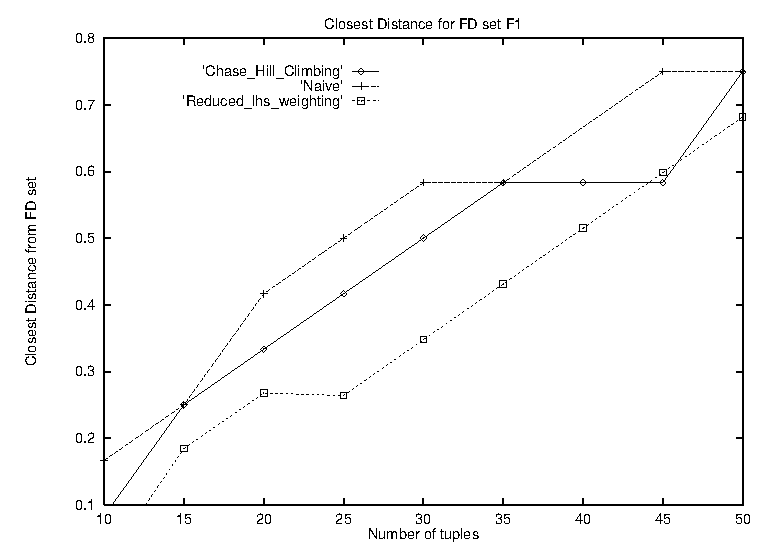
\includegraphics{figures/f1_result.eps}}}
\caption{\label{graph:4.1} {Closest Proximity for FD set $F_1$ across a number of different weighted relations}}
\end{figure}

\smallskip

\subsection{Analysis of the Chase results}\label{subsec:chase_res}
\index{Chase Procedure!Analysis of use}
Simulations showed that the chase 
procedure outperformed
the naive approach, on average, by an increasing margin as the number of
tuples within a randomly generated relation increased. This margin became
slightly larger at higher domain sizes within relations. Obviously, as the
tuple and domain size are increased, the chase procedure becomes more 
effective due to the increased probability of there being more redundant 
values to remove. We can see in Figure~\ref{graph:4.1}
that if there is a bias towards having more indefinite cells in attributes
which are present in the right hand side of FDs (or fewer indefinite
cells in the left hand side, by symmetry) then
the closest proximity for both the naive and chase approaches are better
than an even weighting of indefinacy in left and right hand sides. The
chase procedure is also more effective 
at an earlier stage, evidenced by the {\em Reduced\_lhs\_weighting}
line in Figure~\ref{graph:4.1}. An increased number of indefinite
cells in attributes 
on the right hand side of FDs implies that there may be more values which
may lead to unnecessarily low ND satisfaction (i.e. each ND will have a 
larger branching factor) which can now be removed by the chase heuristic.
Our simulations show the increased efficacy of the chase in such cases.
A larger indefinite cell arity also implies that the chase will have more
values to remove and therefore perform even better. In the case of reducing
the weighting of indefinite cells of the left hand side of FDs, a naive
approach performs much worse than in an evenly weighted relation due to
there being fewer indefinite cells from which it can select different
values, thereby preventing much variation of the partitioning on the NDs 
in a relation which might otherwise occur. Fewer possible worlds are
present in such biased relations though there are still too many to
consider applying a naive approach alone.
Conversely, a reduced
weighting of indefinite cells in the right hand side of FDs also
produces better results than an even weighting of indefinite
cells. This was simply due to the creation of more partitions.
As expected, and in contrast to our work in Chapter~\ref{chap:numdep}
on evolving relations, we did not find a
significant difference between using BCNF and non-BCNF FD sets in
either case. The fact that an attribute is, or is not, part of a
superkey did not affect the overall proximity to an FD holding
within a randomly generated indefinite relation. This may not
necessarily be the case for real-world data, where the presence of a
key may suggest a closer proximity to dependency satisfaction.
\medskip

Figure~\ref{graph:4.2} shows results for
$F_3$ = $F_1 \cup \{ BD \to A \}$. For this relation
the chase procedure performs poorly, on average, with respect to the
naive technique. We believe this is due to the interference of the attributes
within the FD set having attributes determining and being determined by
each other which reduces the application of the chase heuristic.
 We note however that the best results within a batch obtained by both
the naive and the chase and hill climbing are increasingly similar as
relation size increases. We reiterate that the chase and hill climbing
approach requires far fewer worlds.

\begin{figure}
\centerline{\scalebox{0.7}{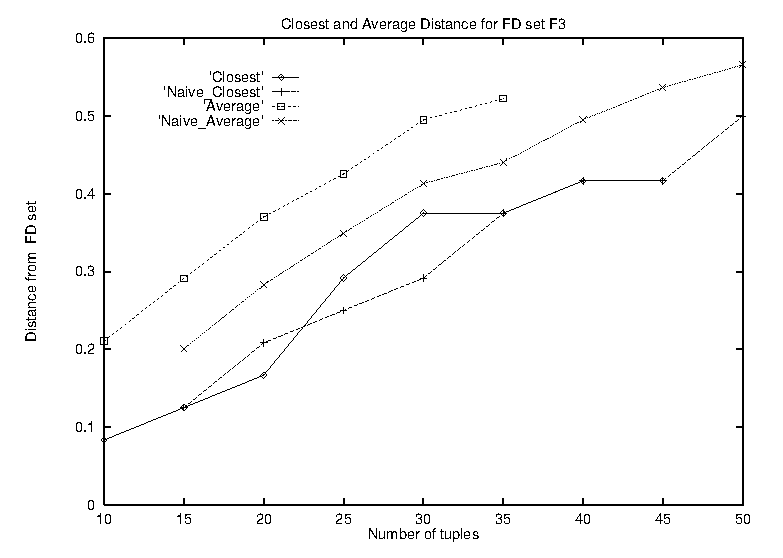
\includegraphics{figures/f3_result.eps}}}
\caption{\label{graph:4.2} {Closest and Average Proximity for FD set $F_3$  }}
\end{figure}

\begin{figure}
\centerline{\scalebox{0.7}{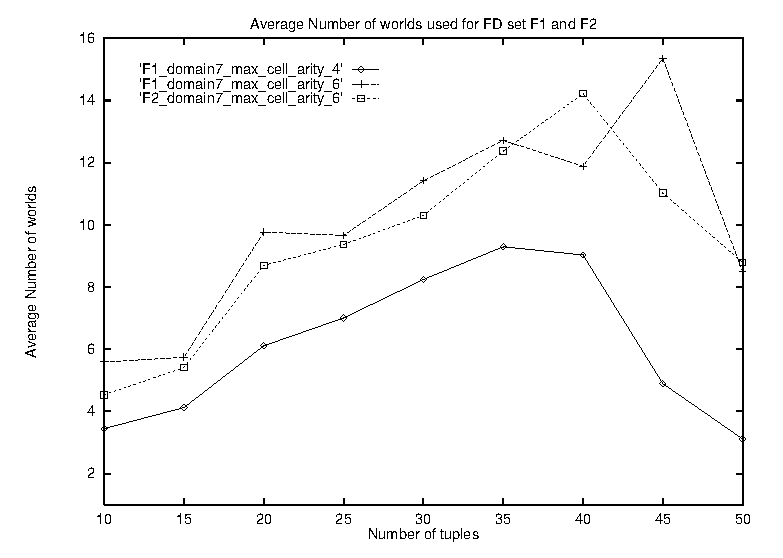
\includegraphics{figures/worlds2.eps}}}
\caption{\label{graph:4.3} {Average Number of Worlds required by
the chase and hill-climbing approach}}
\end{figure}

In Figure~\ref{graph:4.3} we see that, for both FD set $F_1$ and 
$F_2 = \{ A \to B, B \to C, C \to D \}$, as the number of tuples
increases there is a slight peak, after which further increases in the number
of tuples results in a fall in the average number of worlds required.
This is based on every relation within a batch having a fixed domain
size $d$ and an indefinite cell maximum arity, reaching a point where it is
likely that any further increases in the tuple size will lead to the
satisfaction of the numerical dependency set with each ND left hand
side determining $d$ branches and so fewer worlds are required before any 
attempts to apply the chase returns an undefined relation implying that
nothing better can be found. The peaks in Figure~\ref{graph:4.3} were
reflected in the values 
of $\alpha$ returned by our bootstrap technique, corroborated by
Figure~\ref{graph:bj1}. In our
application of the bootstrap, as the relation size of a random relation 
is increased and the domain size is held constant, the sampling will also
reach a point where the variance in the samples amongst the randomly
generated possible worlds is reduced due to most possible worlds 
satisfying the NDs each with a branching factor close to their domain
size. This is likely to also be the case for very large real world
indefinite relations.

\medskip

Given that all of our test data was uniformly randomly generated, with
a bias to or against indefinacy in specified attributes if desired, we
remark that the results echoed the general behaviour
presented here. The average number of worlds required in
Figure~\ref{graph:4.3} emphasises the efficiency of the chase and
hill-climbing over naive procedures.
The lack of indefinite information within databases in daily use prevent
grander conclusions on the efficacy of the chase, where it may have
wider use, particularly with respect to larger relations. For
example, if a database required only indefinite 
information in an attribute on the right hand side of a given FD and
the domain size was small with respect to the database size then the
chase would be an effective heuristic.

\subsection{Changing Bias of indefinite information}\label{subsec:cp_bias}
\index{indefinite relations!Changing bias}
We now briefly discuss differences within resampling for relations
with different bias of indefinite cells in the relation, following on
from the discussion of bias in the previous section. 
Experiments exemplified the importance of how the definite cells
satisfy ND sets; if the definite cells in an indefinite relation
satisfy ND sets which are closer to FD sets then we found a larger
overall variance in our possible worlds.
This is
explained due to the definite cells themselves being further from or
closer to FD set satisfaction which implies, respectively, a smaller
or larger change in proximity within the lattice of NDs. This was
more significant for bigger relations, with a larger domain size and
hence a larger lattice.

\smallskip

In Figure~\ref{graph:cp_hist1} we provide a histogram of
2000 bootstrap replications for a relation with 20 tuples, 
10 attributes and 10 FDs, each with the same singleton left hand side A
and a different singleton right hand side B$_1$, $\ldots$, B$_9$.
The relation has a single partition on A and for each B$_i$ 50\% of
the tuples are indefinite.
We emphasise that more indefinite cells on the left hand side of the
FDs decrease the variance due to each left hand side indefinite value creating
new partitions on attribute values whilst more indefinite cells
on the right hand side of FDs increase the variance. Obviously, the arity of
indefinite cells and intersections of values temper the change in
variance. 


\begin{figure}
\centerline{\scalebox{0.7}{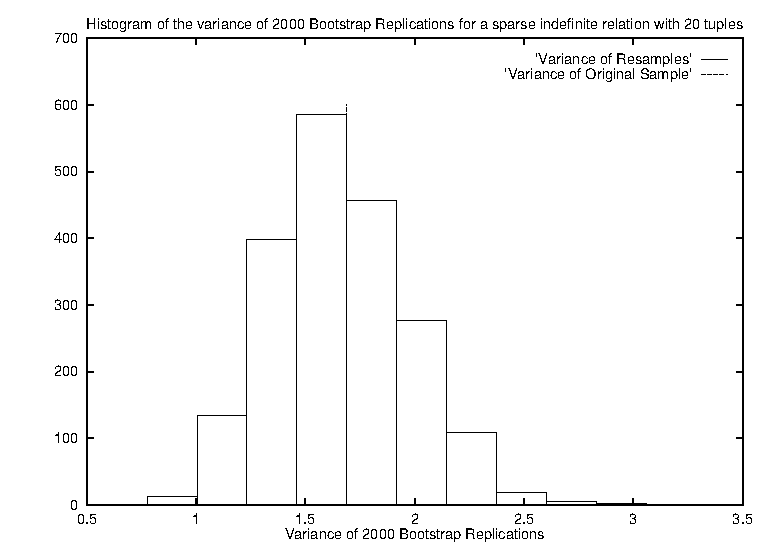
\includegraphics{figures/var2000rel6w25.eps}}}
\caption{\label{graph:cp_hist1} {Histogram of 2000 bootstrap
replications of sample size 25 for a 20 tuple relation and 10 FDs,
with lhs attributes definite and rhs attributes sparse (in FD set) in
indefinite cells}} 
\end{figure}


\subsection{Finding a suitable sample size}
\index{Resampling!Incremental}

Our use of the bootstrap procedure was found to provide a suitable
upper bound on the number of worlds required by our algorithms. We
have explained how the dynamic resampling relies on the variance of ND
set satisfaction amongst possible worlds in the sample to infer when a
larger sample is not required.  The fact that this provided an upper
bound for our algorithms justifies its use. 
As the sample size grows, highlighted in
Figure~\ref{graph:conlim}, there is a reduction in variance between
successive iterations. The non-parametric nature of the resampling is
shown to be useful in that the empirical confidence limits for
the bootstrap process are
shown to converge for the distance measure of an ND set. Determining
confidence intervals with the bootstrap is discussed in Appendix~\ref{app:sim_meth}.


\begin{figure}
\centerline{\scalebox{0.7}{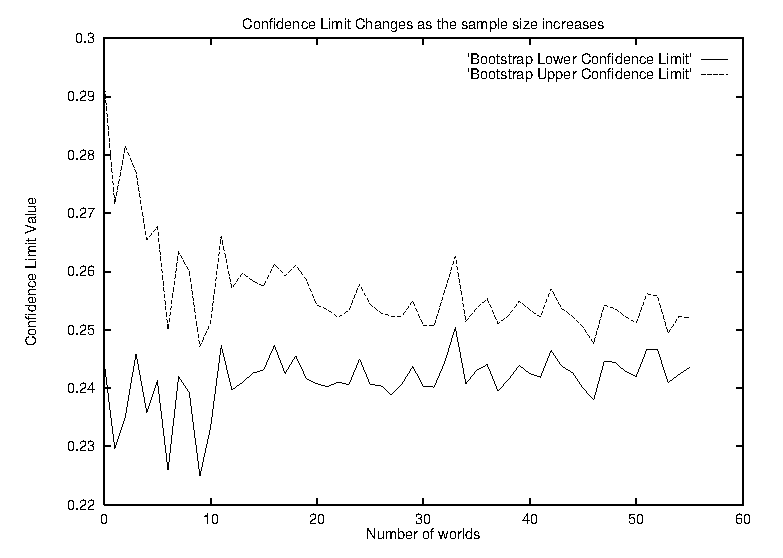
\includegraphics{figures/efronlimit60.eps}}}
\caption{\label{graph:conlim} {Empirical bootstrap percentile
 confidence limits shown to converge for the distance measure of ND sets}}
\end{figure}


A problem with the bootstrap is also discussed in \cite{de83}. It
seems to occur when there is very little variation in the range
of values in the sample data. For instance, it may be the case that
we have an indefinite relation which for a given FD set is such that
nearly all possible worlds satisfy this FD set. Bootstrap sampling
on this data set would be judged to have a very high accuracy,
based on the empirical lack of variation found in the samples.
\cite{de83} says this would be incorrect. The bootstrap will always
perform badly when there is an indefinite relation
with only one or few worlds which we consider to be {\em good} in
the context of approximating FD sets.
Indeed, we do not say that the bootstrap performs badly, it merely
creates an average of the branching values based upon sampling with
replacement from the original subsample. This will always be a good
reflection of the average branching values in the ND set unless the
original $n$ samples are not a good reflection of the true values
in the relation.

Note that the bootstrap procedure can not be used to provide any
indication as to whether there is, or is not, present a very good
approximation to an FD set, or an FD set itself within the relation.
It will only provide an indication of this when there are a large 
number of very good FD sets. Therefore we can state, obviously:
\begin{enumerate}
\item If the values of the Bootstrap when a fixpoint is reached
are functional or near functional then the majority of possible
worlds will satisfy the dependency set functionally or nearly functionally.
\item If the values of the Bootstrap are not
nearly functional in proportion to the size of the relation this
indicates that most of the definite worlds are poor in terms of
satisfying the specified FD set close to functionally.
\end{enumerate} 

We can see from this that the Bootstrap is an averaging mechanism.
The question of why the bootstrap provides an upper bound remains.
The chase and hill-climbing algorithm exits if the chase heuristic
returns an undefined relation for the current highest found ND set,
$N_{\top}$, in
the lattice. This implies that the indefinite relation is unable to
satisfy any ND sets above $N_{\top}$. Given that this generally occurs
before reaching the limit $\alpha$ (provided by the bootstrap) it
seems reasonable to propose that the variance across the possible
worlds of an indefinite relation, in terms of ND set satisfaction,
is a naive statistic and our hill-climbing and chase heuristic method
is sufficient to reach a {\em good} approximation before examing
$\alpha$ initial points.  The correspondence between the heuristic and
the changing upper limit, due to changing variance of ND set
satisfaction in indefinite relations, is to be expected and its usefulness
is highlighted in this work.


\subsection{A Comparison with Jackknife
Resampling}\label{subsec:cp_jackcomparison}  
\index{Resampling!Jackknife}


The strategy of the jackknife is to remove a single data point from each
resample. This allows the creation of $n$ jackknife resamples from an
original sample of size $n$.  The bootstrap provides additional flexibility
in that the sample is made up of any values uniformly and randomly selected
with replacement from the original and, additionally, is not limited to
$n$ resamples.  In our process the number of worlds required is increased
until a fixpoint is reached. Using the jackknife as the worlds reach a
large number $q$ we are constrained to $q$ resamples, each of size $q-1$.
Under the bootstrap application we have a fixed number of resamples which,
in the majority of cases,
will increase to a sample size that is smaller than the $q$ required by the 
jackknife. We found
that the results were very similar for both the bootstrap and jackknife, 
highlighted in Figure~\ref{graph:bj1}, 
despite our use of the bootstrap conducting fewer replications than the
jackknife at large sample sizes. Based on the dynamic nature of our
resampling often requiring large sample sizes it is therefore much
more efficient to use bootstrap and not jackknife resampling. 
Figure~\ref{graph:bj1} also presents
the falling limit of the fixpoint as the domain size is held constant but
the tuple size increases, due to a reduction in variance within
possible worlds as the relation size grows, highlighted in
Figure~\ref{graph:conlim}.


\begin{figure}
\centerline{\scalebox{0.7}{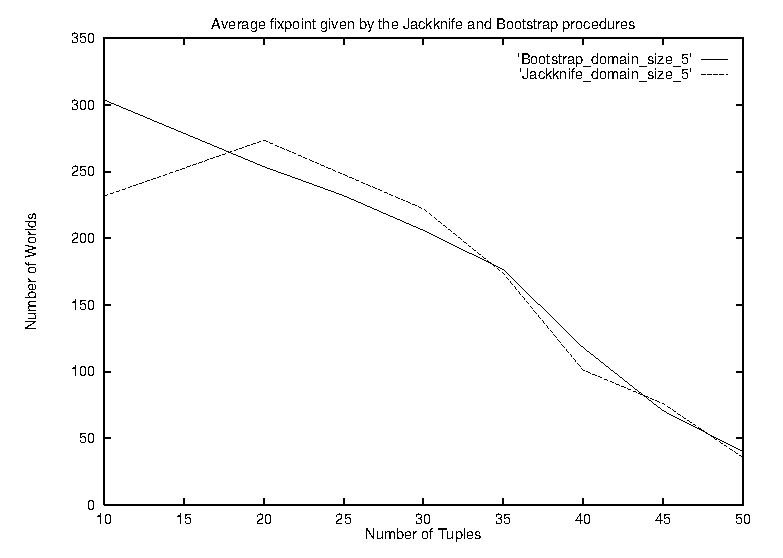
\includegraphics{figures/bootjackav.eps}}}
\caption{\label{graph:bj1} {Average Number of Worlds given as 
upper bounds by the Bootstrap and Jackknife techniques for a fixed domain
size 5}}
\end{figure}

Additional results are given in appendix~\ref{app:con_prob} for
different FD sets; they parallel the results presented.

\subsection{Real-World Applications}\label{sec:cp_apps}

In \cite{inv91} we are shown how indefinite information may be used to
represent a possible schedule. Our approach allows us to discover an
approximation to an {\em ideal} relation, {\em ideal} being a relation
which satisfies
a set of FDs. NDs are a useful tool in this context and indeed 
schedule representation within relational databases would be enhanced with
their use. Any approximation
provided by our system for a relation can be analysed by the system
users. The schedule which is produced by this, or any other, system can
be studied with respect to the result of our procedures. If there are
FDs which are not satisfied within the relation and these are less
functional than those provided as output by our chase and hill-climbing
approach we can assume a superior schedule exists. The Bootstrap
parameters will also tell the user valuable information on the
variance and mean of the possible dependency sets which will enhance
their knowledge of the indefinite data within the relation.

\medskip

Section~\ref{sec:conprob} briefly mentioned the relationship between
the use of indefinite information and constraint logic programming. We
can easily see that a domain constraint, stating for example $p$ = 4
or $p$ = 5 or $p$ = 6, can be represented within a relation with an
indefinite cell of the form $\{ 4, 5, 6 \}$. A FD can then be used to
constrain $p$ to just one of these values. In such a way we note that
various constraint problems can be encoded within a database,
motivating the use of indefinite information.

\medskip
 
NDs, together with the metric presented in
Section~\ref{sec:cp_approx}, are applicable 
within any relational database for approximating and comparison of FD sets.
In a data mining environment this could be used for contrasting approximations
in relations over the same attributes which may be in use at different
locations. The use of our dynamic resampling procedure, presented in
algorithm~\ref{alg:blimit}, has applications wherever a non-naive
sample size is required to be representative of a population. The
approximate fixpoint can be refined empirically based upon the data
set and the application to a point where dynamic resampling can be
applied to numerous problem instances within the same domain.
 

\section{Discussion}\label{sec:cp_disc}


We have described how the representation of indefinite information is a 
valuable extension to relational databases, following on from the work
in \cite{inv91,vn95}. In addition to this we 
note that NDs suitably generalise FDs
both in a database design context where they may be used in their
own right when an FD is too strict \cite{gm85b}, or within the context of their
usage in this chapter where we have used them to approximate FDs based
on all possible NDs which may hold within a relation for a given set
of FDs forming a complete lattice.  The use of NDs extends the work of
\cite{vn95} 
where relations which do not satisfy the constraint set functionally are
said to be {\em unrealisable}. In many dependency data mining applications,
which range from data summarisation to learning within decision trees \cite{psm93}, we may wish to obtain a numerical value, between 0 and 1, denoting how close a set of 
FDs are to being satisfied; the metric, presented in
Chapter~\ref{chap:numdep}, and used in indefinite relations, achieves
this. 
The consistency problem for relations with indefinite information is
widely known to be NP-complete. Therefore we cannot expect to
develop a polynomial time based solution unless $P = NP$ or the database is
restricted as in \cite{vn95}. Our approach
does however introduce an interesting new technique based on sampling,
extending the bootstrap to providing useful approximations for
problems such as the consistency problem. Essentially, it is based on
extracting a representative sample and inducing assumptions on the 
complete indefinite relation based on the variance within the samples, and
subsequently the Bootstrap resamples. We have shown this to provide us
with valid upper bounds. The dynamic resampling approach we have
presented may be applicable to other NP-complete problems where an
approximation to a solution may be useful, using a sample of the data.

\medskip

The simulations have shown that our procedure can provide useful
approximations to FD sets in the form of ND sets for any indefinite
relation. We compared different weightings of indefinite information within
a relation and showed that as a relation approaches what \cite{vn95}
refer to as a {\em good database}, one without indefinite information
in the left hand side of the dependencies, then the chase procedure for
NDs becomes more effective. The efficacy of the chase heuristic, extended in
this work to apply to NDs, over naive methods is shown in that
best result achieved within a batch is generally found when using the 
chase and hill-climbing procedure, evidenced in Appendix~\ref{app:con_prob}. 
Also, on average around 10\% of 
the worlds used in 
a naive approach are required by a chase and hill-climbing approach.
The bootstrap provides a suitable upper bound with, on average, 
less than 1\% percent of relations generating the number of worlds it
takes to reach a fixpoint when using chase and hill-climbing technique.
No simulations or empirical discussion is provided in related work,
\cite{vn95,inv91}. \cite{imi91} presents a theorem (Theorem 3) which
states that no chase-like procedure, namely an algorithm which
examines a fixed number of tuples at a time, exists to completely
remove all redundant values in relations with indefinite
information. \cite{vn95} notes that other algorithms, however, may
achieve this.

\medskip
\index{NP-Complete}
\index{Phase Transition}
A greater understanding of the behaviour of NP-complete problems
is provided in \cite{slm92,msl92}.  \cite{ckt91} introduces
the details of {\em phase transitions} occurring where NP-complete
problems become really hard.  These areas are dense in local
minima so that there are many near solutions which the search procedure
follows.  On either side of this critical boundary the 
problem distribution tends to be either over- or under- constrained.
For both of these cases the search is cut off quickly and the 
probability of success tends to 1 and 0 respectively. Phase
transitions  occur from a region where
most problems are easy and soluble to a region where most are
easy but do not contain a solution. However, as \cite{sg94} note, there are
certain {\em exceptionally} hard problems on either side
of the phase transition which are much harder than those occurring
inside the phase transition. A study of these exceptionally
hard problems shows that they are the ones most likely to
encounter an insoluble subproblem at an early stage. \cite{ckt91}
points out that complex systems with many
interacting values can often be understood at the
macroscopic level which characterises the whole system.
We should seek, similarly, 
to understand where such transitions occur for the consistency
problem in further work, as they might provide a useful insight into
the representation of indefinite information in relations such as a
suitable frequency of indefinacy.

\medskip

Though we
have analysed our algorithms behaviour empirically, an approach advocated in
\cite{hoo94}, we consider a theoretical analysis to be an interesting
avenue for future 
research, in particular for algorithm~\ref{alg:blimit}, our dynamic
bootstrap application. Other approximation techniques for the
consistency problem, such as finding a suitable subset of an
indefinite relation which satisfies an ND set and then adding tuples
to this in a hill-climbing fashion would also be interesting to study,
both empirically and theoretically. We would also like to see results
of dynamic resampling gained from application in other domains.




\chapter{Temporal Data Mining for Temporal Property
Detection}\label{chap:templog}

In this chapter we introduce a temporal logic based upon sequences
with NDs, possibly representing time series functions, for temporal data
mining purposes. We show how temporal properties may be formalised
within this logic and used for temporal data mining.
\smallskip

In Section~\ref{sec:tl_intro} we introduce and motivate this
work, stating why we focus on NDs. Section~\ref{sec:tl_why} follows
with a discussion of why
properties are useful for temporal data mining, concentrating on the
ability to succinctly characterise temporal behaviour. In
Section~\ref{sec:tl_nd} we briefly present NDs in a temporal database
and follow this in Section~\ref{sec:tl_tsa} with a presentation of
time series analysis. We provide this for two reasons. Principally
because our logic uses some time series analysis functions and
secondly as a comparison between our work and a standard time series
analysis that may be performed on a temporal database, noting that the
branching factors of an ND
in a temporal database may be viewed as a time series. In the next
chapter we shall see some results from applying our logic for temporal
property discovery just to time series.  Section~\ref{sec:tl_relations}
provides an introduction to temporal sequences upon which our logic is
based. In Section~\ref{sec:tl_ndltl} we formally define our temporal
logic. Finally, in Section~\ref{sec:tl_properties} we define some temporal
properties and discuss the intuition behind attempting to discover
these properties from a temporal database. \cite{jmw96} state that,
``the task of data mining can be seen as the problem of extracting the
interesting part of the logical theory of a model.'' We consider
specific properties to represent interesting patterns within our logic.
We conclude with a
discussion of the open problems that remain in~\ref{sec:tl_disc}.

\section{Introduction}\label{sec:tl_intro}
\index{snapshot!relation}
In Temporal Databases we
may view each state at time point $t$ as a snapshot of the database. 
Over a series of time points, taken at fixed intervals, each snapshot 
may satisfy changing
ND sets which may model temporal relationships previously unknown to
the database user. We assume the time intervals are fixed for clarity
within the discovery process though it would be feasible to {\em unfold}
time points over different size intervals into a fixed representation.

\smallskip

The sets of points satisfied by the ND sets across time form a time
series. We introduce in Section~\ref{sec:tl_ndltl} a temporal logic of
sequences to model aspects of
time series statistics and present them as ``properties'' of the
temporal database. The modal operators are extended from the temporal
logic operators of safety, implying at all future points, and
guarantee, implying at some point in the future, to implying all
subsequences of size $n$ and some subsequence of size $n$, respectively.  
In this way we use these operators to characterise
the temporal database with such statements as, for example, ``all
sequences of 100 days contain, at some point, a downward trend of 30
days.''  The size of the sequence may pertain to a relevant unit of
time, such as a month or a week, or length relating to behaviour of
the data in question. We also define the $\leadsto$ temporal operator which
represents a non-strict temporal ordering in that overlap is allowed.
The expression of temporal behaviour within a succinct logical
form allows for both the discovery of new knowledge and the machine
understandable form of well understood behaviour within the temporal
database. 
This has applications both in knowledge discovery and
decision support. 
\smallskip

We show how our logic may be applied to study time series for
property discovery. In Chapter~\ref{chap:tempresult} we give examples
of properties found in temporal
datasets which may be viewed as temporal relations. Loosely speaking,
properties are formulae within our language which satisfy a template
such that properties of a particular nature may be classified as, say,
conditional or persistent properties. We motivate their use in
Section~\ref{sec:tl_why}. 
We also provide
results showing interesting properties
discovered on stocks within the FTSE 100 over different
time periods. Additionally, we make use of the resampling technique
known as the {\em moving blocks bootstrap}. From an input time series we
randomly sample blocks, or in this case sequences of a size $n$, and
append the sequences to the resampled series as they are selected
until we have a resampled series of equivalent length to the original
series.  
The resampling destroys long term relationships whilst preserving
relationships of a size less than $n$, allowing us to
look for short range properties which may hold in various time series.
We apply our property discovery
algorithms to these and the original sequences and provide examples of
interesting,
useful and previously unknown properties which hold, satisfying all of
the criteria for successful knowledge discovery. We do however stress
that properties discovered may 
require expert examination for validation as a contribution to
knowledge. This is a key point for all knowledge discovery systems
\cite{fps96,man97}. We conclude in
Section~\ref{sec:tl_disc} with a
discussion proposing the inclusion of these techniques into DBMS.

\section{Why do we need properties for Temporal Data Mining?}\label{sec:tl_why}
\index{Rule Discovery}
\index{Events}
\index{Temporal Logic Properties}
\index{Properties|see{Temporal Logic Properties}}

There has been much work on properties holding in temporal logic, upon
which the seeds of this work lie, most notably \cite{mp92}. Properties
in temporal logic have arisen out of the application of temporal logic
to computing. Transition rules in a program allow for properties to be
specified. For example, the standard notation would use $\Box p \to
\Diamond q$ to denote that at all future points $p$ holds ($\Box p$)
which implies
that at some point in the future $q$ holds ($\Diamond q$) and this is
referred to as a
{\em response to insistence} property. We redefine connectives and
properties in
our logic so that we may discover various forms of response and
persistence rules for temporal sequences. We define a response rule as
\resp{n}{m} $\sigma$ which implies that all subsequences
of size $n$ ($\bm^n$) contain a sequence of size $m$ (\diam$^m$) which
satisfies $\sigma$, and a persistence rule as \pers{n}{m} $\sigma$  
stating that for a sequence of size $n$ all of its $m$ length subsequences
satisfy $\sigma$, where $m \le n$.
The contribution of this work is the use of property discovery in a
temporal logic relating to subsequences for discovering relationships
about NDs, the atoms of our logic, in temporal databases.
	
\section{Numerical Dependencies in a Temporal Database}\label{sec:tl_nd}
\index{Numerical Dependencies!in a Temporal Database}
In a Temporal Database each snapshot at a particular time may satisfy
a set of NDs. We assume that the ND set is specified via an attribute
set template provided by the database user, though we note that it is
possible to ``mine'' the relation for NDs blindly as detailed in Section~\ref{sec:nd_datamine}.

\subsection{Temporal Relation Sequences}\label{sec:tl_relations}
\index{Temporal Sequences}
\index{Sequences|see{Temporal Sequences}}


\begin{definition}[Temporal Relation Sequence]
\begin{rm}
A {\em relation sequence} (temporal database) $\Delta$ over R is a
finite set of 
relations over R with $\Delta$ = $\{ r_0, r_1, \ldots, r_n \}$,
indexed chronologically $0, 1, \ldots, n$ from an initial point 0 and
having a final point $n$, each state corresponding to a time point a
fixed interval apart from its previous and next value. $\quad\Box$
\end{rm}
\end{definition}

We assume that our relation sequence, equivalent to a temporal
database, is a collection of
relations which are linearly ordered. As such we infer within our
logic that time itself is linearly-ordered. At each moment there is
only one possible future moment. 
Our underlying sequence is finite. This is natural given that the
input for the
data mining procedures is a finite sequence of relations.


\subsection{Time Series Analysis and Numerical
Dependencies}\label{subsec:tl_tsa_nd}
\index{Numerical Dependencies!and Time Series Analysis}

We now briefly present the relationship between time series and NDs.

\smallskip

The simple example in tables~\ref{tab:1} and~\ref{tab:2} for
a relation $COLLEGE(C,S,T)$ over two years where $C$, $S$, and $T$
represent course, student and tutor, respectively, highlights possible
transition in a temporal database. The change in ND set satisfaction
for the ND set = $\{ C \to^k S, C \to^k T \}$ from $\{ C \to^3 S, C \to^2 T \}$
to $\{ C \to^4 S, C \to^1 T \}$ may be an indicator of both increasing
student numbers on courses whilst at the same time implying that
tutors have more work to do on a course. This information could be
represented in a single relation if timestamps were attached to each
tuple.

{\line
\begin{table}[ht]
\begin{minipage}[b]{7.2cm}
\begin{center}
\begin{tabular}{|c|c|c|} \hline
 C & S & T \\ \hline
 b11a & Paul & Mark \\ 
 b11a & Tina & Mark \\
 b11a & Fred & Robin \\
 b151 & Paul & Robin \\ \hline
\end{tabular}
\end{center}
\caption{\label{tab:1} 1997 student intake records}
\end{minipage}
\hfill
\begin{minipage}[b]{7.2cm}
\begin{center}
\begin{tabular}{|c|c|c|} \hline
 C & S & T \\ \hline
 b11a & Tom & Mark \\
 b11a & Dan & Mark \\
 b11a & Louise & Mark \\
 b11a & Jim & Mark \\
 b151 & Jim & Robin \\ 
 b151 & Jose & Robin \\ \hline
\end{tabular}
\end{center}
\caption{\label{tab:2} 1998 student intake records}
\end{minipage}
\end{table}
}


Clearly, the change in ND set satisfaction may be viewed as a
time series. For example, $C \to^{16} S$, $C \to^{20} S$, $C \to^{27} S$ may
be viewed as a time series of points $16,20,27$ assuming a fixed time
interval between insertion.

\medskip

The requirement that for a template of NDs provided for a relation the
ND set only changes on the branching factor may be seen as
restricting. Schema evolution \cite{oe92,rod94} may remove an attribute from
the relation thereby making an ND in a given set null and void. We
assume the following: (1) For the input provided the schema is fixed,
and (2) changes in the schema can be assessed by separate mining
processes on two separate relation sequences, one before and the other after
any schema update.  


\section{Time Series Analysis}\label{sec:tl_tsa}
\index{Time Series Analysis}
We now provide a brief overview of time series analysis. In
Section~\ref{subsec:tl_tsabasic} we discuss research on time series
analysis and emphasise areas which our work may be considered as
contributory to. Then in Section~\ref{subsec:tl_tsadefs} we provide
definitions of standard functions used within linear time series
analysis which are embedded within our logic.

\subsection{Time Series Analysis: Basics}\label{subsec:tl_tsabasic}

The goal of time series analysis is to model an observed system so
that its future behaviour may be predicted \cite{wg94}. We discuss
both traditional time series analysis and new techniques, such as the
use of neural networks, and then relate this to our work. Having read
this section the reader will fully appreciate the statistical
functionality we incorporate into our logic, presented in
Section~\ref{sec:tl_ndltl}. We assume familiarity with the statistical
functions, such as variance, covariance, correlation, autocorrelation
etc, defined in Section~\ref{subsec:tl_tsadefs}.

\medskip

The standard methodology for analysing a time series is to decompose
the series into trend, seasonal and irregular components, each of
which may be expressed as individual functions of time. \cite{wg94}
demarcates the difference between understanding and learning from a
time series as that of applying explicit mathematical insight for
model creation to that of using
learning algorithms to emulate the behaviour of the time series. Our
goal is closer in spirit to understanding the sequence, using
properties to achieve this. For linear and stationary time series one
of the most popular techniques is to create an autoregressive (AR) model,
of the following form for the Mth order AR model, where the first $M$
autocorrelations determine the coefficients \cite{end95}:
\begin{displaymath}
x_t = \sum_{m=1}^M a_m x_{t-m} + e_t
\end{displaymath}
where $e_t$ represents noise and $a_m$ the autoregressive
coefficients for $x_t$ on $x_{t-1}$, $x_{t-2}$, $\ldots$, $x_{t-M}$; $e_t$
is assumed to have expectation 0 and is independent of previous
values. Moving Average (MA) models can also be characterised by
autocorrelation coefficients describing how values $\tau$ steps apart
co-vary with each other. \cite{ko90} remark that autocorrelation
coefficients for large lags are unreliable for model
identification. We found this to be true within our logical
representation and adopted their advice of restricting lags of a time
series with $n$ points to lags up to $\frac{n}{4}$. This seemed to be
a sensible 
restriction across all time series sizes, given that the reliability
of the lag values decrease for higher lags and that we are using
sequences of a size chosen by the user which may be arbitrarily short.

\medskip

AR and MA models may themselves be combined to form ARIMA models,
denoting Autoregressive Integrated Moving Average models, integrated
implying that we are dealing with a stationary time series, after {\em
differencing}.
We omit a full discussion of model selection,
provided in
\cite{ko90,end95}, suffice to say that ARIMA models have had the
greatest impact on linear time series analysis. Other aspects of time
series analysis are the Yule-Walker equations which allow the
autocorrelation coefficients of a time series to be expressed by
autoregressive coefficients. This is simply understood given their
definitions; see \cite{ko90}. The restriction of analysis methods to
linear time series may cause problems. Two approaches to combat this
are:
\begin{enumerate}
\item Approximating a system with more than one linear model, known as
local linear modelling. \cite{wg94} state that many regions must be
selected if the nonlinearity is of a quadratic degree or greater.
\item The use of differencing to remove trend. \cite{naze88,end95}
comment that most nonstationary time series, where nonstationary
implies a trend, can be changed to
stationary time series by differencing once or twice. Given a series
\series{n} we obtain the first and second order differenced series by 
$y_2 - y_1, y_3 - y_2, \ldots, y_n - y_{n-1}$ and 
$y_3 - 2y_2 + y_1, y_4 - 2y_3 + y_2, \ldots, y_n - 2y_{n-1} +
y_{n-2}$, respectively. \cite{naze88} comments that most economic time
series are stationary after at most second order
differencing. \cite{raf99} refers to differencing as {\em momentum}.
\end{enumerate}

Our logic incorporates aspects of local linear modelling by breaking a
time series into sequences which may then be linearly regressed within
the sequence; we also allow differencing within our
logic. \cite{naze88} states that ``the best practical approach in
examining a series is visual examination of the plot of the series.''
It is a key intention of this work to provide a definite contribution
to any visual examination of a time series.  

\medskip

Nonlinear time series have most recently been the subject of analysis
by neural networks. \cite{wg94} stresses the importance of
differentiating between learning for model discovery and simple
memorisation. The latter occurs when the data is overfitted and
prediction relies too heavily on previous values (including noise)
rather than looking for a model. The complexities of non-linear time
series analysis are outside the remit of this work. We believe that
the application of sequences to differenced, and/or moving averaged,
time series implies that our
procedures can still obtain meaningful properties from such non-linear series.
This is due to the fact that though there may not be any global linear
properties 
of the time series our use of sequences breaks the time series up and
within these sequences there may be linear behaviour allowing for
potentially interesting knowledge discovery. \cite{cl96b} notes some
strengths of local regression stating it adapts well to high
curvature, can be tailored for many distributional assumptions, and is
easy to understand and implement.

\subsection{Time Series Analysis: Definitions}\label{subsec:tl_tsadefs}
\index{Time Series Analysis!Definitions}

We now present the standard statistical functions used within linear
time series analysis \cite{ko90}.
\index{variance!of a time series}
\begin{definition}[Variance]\label{def:var}
\begin{rm}
Given a time series $x$ of length $n$, its variance is written as
$var(x)$ where
\[
var(x) = \frac{1}{n-1} \sum_i^n (x_i - \mu)^2
\]
We assume that the series is stationary having a mean value $\mu$.$\quad\Box$
\end{rm}
\end{definition}

\index{standard deviation!of a time series}
\begin{definition}[Standard Deviation]\label{def:sd}
\begin{rm}
Given a time series $x$ its standard deviation is $\sigma_x$ where 
\[
\sigma_x = \sqrt{var(x)}\quad\quad\Box
\]
\end{rm}
\end{definition}
\index{covariance}
\begin{definition}[Covariance]\label{def:covar}
\begin{rm}
Given two time series $x$ and $y$, both of length $n$, their
covariance is written as $cov(x,y)$, where
\[
cov(x,y) = \frac{1}{n} \sum_i^n (x_i - \mu_x) (y_i - \mu_y)
\]
We assume that the series $x$ and $y$ are stationary with mean values
$\mu_x$ and $\mu_y$, respectively.$\quad\Box$
\end{rm}
\end{definition}

Covariance is a measure of the linear association between two variables.
The strength of the relationship unfortunately depends on the unit of
measurement used and so to avoid this we introduce the correlation
coefficient.
\index{correlation coefficient}
\begin{definition}[Correlation Coefficient]\label{def:correl}
\begin{rm}
Given two time series $x$ and $y$ the correlation coefficient
$cor(x,y)$ is
\[
cor(x,y) = \frac{cov(x,y)}{\sigma_x \sigma_y}\quad\quad\Box
\]
\end{rm}
\end{definition}

The regression coefficient determines the slope for a series of values
where $y$ is time when dealing with temporal sequences.
\index{regression coefficient}
\begin{definition}[Regression Coefficient]\label{def:regcoef}
\begin{rm}
Given a time series $x$, the regression coefficient
$reg(x)$ is
\[
reg(x) = \frac{cov(x,y)}{\sigma_y}
\]
where $y$ represents time.$\quad\Box$
\end{rm}
\end{definition}

We note that regression is equivalent to correlation but without
the standard deviation of $x$ in the denominator. Therefore, unlike
regression, 
correlation does not make a distinction between the $y$-value and the
value upon which it is regressed, in our case time. Another process
for determining the trend of a sequence is to use discordance which
sums the value comparisons over all possible pairs of values to
determine trend, defined as: 
 
\index{discordance}
\begin{definition}[Discordance Test]\label{def:disccoef}
\begin{rm}
Given a time series $y$ = $\{$ \series{n} $\}$, we let
\begin{eqnarray*}
q_{ij} & = & 1, \quad\mbox{if}\quad y_i > y_j \quad\mbox{when}\quad j > i \\
       & = & 0, \quad\mbox{otherwise}
\end{eqnarray*}
We define $Q$ as:
\[
Q = \sum \sum_{\!\!\!\!\!\!\!\!\!\!\!i < j} q_{ij}
\]

Now, this series is random under the null hypothesis and since there
are $n$ points in the time series then there are $\frac{1}{2} n(n-1)$
pairs and so the expected value of $Q$, E($Q$) = $\frac{1}{4} n(n-1)$
Our discordance function for a time series $y$ is:
\begin{eqnarray*}
discord(y) & = & 1,  \quad Q < E(Q) \\
      	   & = & -1, \quad Q > E(Q) \\
	   & = & 0,  \quad \mbox{otherwise} \quad\quad\Box
\end{eqnarray*}
\end{rm}
\end{definition}

Autocovariance and autocorrelation are presented as we may wish to
compare sequences of the same time series.
\index{autocovariance}
\begin{definition}[Autocovariance]\label{def:autocovar}
\begin{rm}
Given a time series $x$, of length $n$, its autocovariance of lag $k$
(or lead $-k$) is written as $autocov(x,k)$ where
\[
autocov(x,k) = \frac{1}{m} \sum_i^m (x_i - \mu_x) (x_{i-k} -
\mu_{x})\quad\mbox{where}\quad m = n-k 
\]
We assume that the series $x$ is stationary with mean value
$\mu_x$.$\quad\Box$ 
\end{rm}
\end{definition}

\index{autocorrelation coefficient}
\begin{definition}[Autocorrelation Coefficient]\label{def:autocorrel}
\begin{rm}
Given a time series $x$ the correlation coefficient $acor(x,k)$ is
\[
acor(x,k) = \frac{autocov(x,k)}{\sqrt{var(x)var(x-k)}}\quad\quad\Box
\]
\end{rm}
\end{definition}

\index{cross covariance}
\begin{definition}[Cross Covariance]\label{def:crosscovar}
\begin{rm}
Given two time series $x$ and $y$, both of length $n$, their
cross covariance of lag $k$
(or lead $-k$) is written as $ccov(x,y,k)$ where
\[
ccov(x,y,k) = \frac{1}{n} \sum_i^n (x_i - \mu_x) (y_{i-k} - \mu_y)
\]
We assume that the series $x$ and $y$ are stationary with mean values
$\mu_x$ and $\mu_y$, respectively.$\quad\Box$
\end{rm}
\end{definition}
 
\index{cross correlation coefficient}
\begin{definition}[Cross Correlation Coefficient]\label{def:crosscorrel}
\begin{rm}
Given two time series $x$ and $y$ the cross correlation coefficient $ccor(x,y,k)
$ is
\[
ccor(x,y,k) = \frac{ccov(x,y,k)}{\sigma_x \sigma_y}\quad\quad\Box
\]
\end{rm}
\end{definition}

\subsection{Catalytic Data Mining}\label{subsec:tl_catdm}
\index{Catalytic Relation|see{Catalytic Data Mining}}
\index{Catalytic Data Mining}

Catalytic Data Mining is a term introduced by \cite{HS95} for the data
mining of two or more relations which agree on a common attribute or
more so that the data mining process can be enhanced. We mention it
here given that it applies to NDs in temporal relations. Our data
mining process is such that for a company we can extract NDs from
either an employee or product sales relation and 
then perform the mining on this together with a directly numerical
value such as the stock price. Over time a fall in stock price
combined with little change in an ND in the sales relation each
October may suggest that a sale is held at this time of year to
increase sales.

\subsection{Advantages of a logical approach}
\index{Linear Temporal Logic|see{Numerical Dependency LTL}}
\index{Temporal Logic}
\index{Modal Logic!see{Temporal Logic}}

Standard time series techniques allow us to apply time series functions
to time series naively. This, in turn, may produce useful results such
as a high cross-correlation between two time series. A symbolic
representation of this provides similar information without recourse
to numerical comparison. Therefore our logic is algorithmic and
as such is amenable to symbolic manipulation. This implies that it is
of use within decision support tools and perhaps general data mining
systems.

\medskip

The logic is also flexible so that many
different kinds of relationships and patterns can be expressed in a
very concise form. This is a result of using a high-level logic to
represent desired concepts. 


\section{Numerical Dependency Linear Temporal Logic}\label{sec:tl_ndltl}
\index{Numerical Dependency LTL}

We now formalise our temporal logic for sequences which we refer to
henceforth as NDLTL. Much of the intuition behind sequences follows
from Allen's temporal intervals which we advise reading for a clear
understanding of the use of intervals and sequences in time
\cite{all84}.

\subsection{Temporal Logic}
\index{Temporal Logic}
Propositional Linear Temporal Logic is propositional logic augmented
with the modalities ${\cal S}$ and ${\cal U}$, denoting since and
until, respectively, defined in \cite{ghr94}. For atoms A and B, A ${\cal S}$ B is true at time $t_n$,
if for time $t_0$ where $t_0 < t_n$, if B is true at $t_0$ and for all
points between $t_0$ and $t_n$, A is true. Similarly, A ${\cal U}$ B
is true at $t_p$ if for some $t_q$ where $q > p$, B is true at $t_q$
and for all points between $t_p$ and $t_q$, A is true. 
From these modal primitives further temporal
operators may be defined, of which the principal ones are $\Box$ and
$\Diamond$, implying, respectively, at all future points and at some
point in the future. 
$\Diamond$ A may be defined as {\em true} ${\cal U}$ A, $\Box A$ is the dual
of $\Diamond$ A defined as $\neg \Diamond \neg$ A.  $\bigcirc$ A,
representing {\em nexttime} A, may be defined as {\em false} ${\cal U}$ A
\medskip

A logic may be created due to concerns that there are inadequacies
within previous logics to represent various kinds of informal argument
\cite{haa78}. We wish to represent arguments representing aspects of
time series analysis within a logical form that allows patterns in the
temporal sequences to be represented; a logic is a system for
obtaining answers from $\Delta$ \cite{ghr94}. Our logic is with respect to
sequences of temporal relations, equivalent to the interval
representation of time \cite{all84}.
We modified our logic to contain $\leadsto$ and $\bm^n$ as primitives
with respect to sequences. Formulae of the form $\sigma_1 \leadsto
\sigma_2$ imply that a sequence $s_1$ starts before $s_2$ and
ends before $s_2$ ends, with $s_1$ satisfying $\sigma_1$ and $s_2$
satisfying $\sigma_2$. If a sequence $s_1$ satisfies $\bm^n \sigma$
this implies that all sequences of size $n$ in $s_1$ satisfy
$\sigma$. 

\medskip

Another possible approach would have been to incorporate the time
series operators at the atomic level and apply these within a standard
temporal logic for knowledge discovery. We now show by example some
potential problems with this. A sequence $s$ may satisfy
ccor($\sigma_1$, $\sigma_2$, $k_1$) ${\cal U}$ ccor($\sigma_1$,
$\sigma_2$, $k_2$). Even if we allow the inclusion of such time series
functions we are likely to discover that time series are unlikely to
satisfy a formulae A ${\cal U}$ B without numerous conjuncts leading
to formulae such as A ${\cal U}$ B ${\cal U}$ C ${\cal U}$ A ${\cal U}$
B. The problem with using standard {\em point based} temporal logic
for the discovery of 
such formulae is that they are apt to {\em overfit} the data; in this 
brief example we have A ${\cal U}$ B holding twice. It would be of
more value to be able to represent this fact, which our logic of
sequences achieves in some respect. Standard temporal logic models
atoms occurring at certain time points such as inferring A ${\cal U}$ B over
a period of $p$ time points. This, within a point based
logic, may lead to the discovery of many hundreds of
formula. However, we approach our discovery from the
basis of creating sequences so that we control the granularity of 
property discovery given that we may have to
deal with many hundreds of time points.  Though this may result in
valuable knowledge found we 
believe a sequence based logic results in finding {\em interesting}
knowledge more easily.
Similarly
$\Box A$, denoting at all points in the future A holds in temporal
logic, is unlikely to 
either be satisfied or, if it does, represent interesting
information. Another potential problem is that the discovery of
temporal logic formulae without restriction may often be too complex for
efficient knowledge discovery; formulae such as (C ${\cal U}$ A)
${\cal S}$ (B ${\cal U}$ C) or $\Box$ (A $\to$ $\Diamond$ D). These
formulae themselves do not represent complex behaviour, for example,
the former proposition may hold if C occurs between one or more
occurrence of both B and A. Therefore we choose to
restrict our discovery to search for what we believe are interesting
formulae.
\medskip

These
deficiencies suggest that formulae be verified with respect to
sequences. Therefore, we have modified our modal operators with
respect to sequences. We also introduce $\leadsto$; this is a temporal
ordering operator which allows overlap. We motivate its inclusion
based on the fact that within time series and temporal sequences
strict transitions of properties may not occur. The formalisation of
$\leadsto$ is sufficiently flexible yet restrictive enough to discover
interesting patterns within and across sequences. The requirements
outlined in \cite{ghr94} for the components for specification of a
temporal logic are all provided in our formal definition apart from
allowing our units of time to vary across data sets, though we may
generalise and say that time is the set of integers, satisfied in all
data sets. 

\smallskip

We shall demonstrate, informally, how sequence-based temporal operators
are more appropriate for data mining applications. As we shall see in
section~\ref{subsec:logic_query} our discovery process is
computationally efficient due to our restriction of fixed sequence
sizes which allow for polynomial time knowledge discovery. We assume that we
have as input a finite temporal database; given this it is of minimal
value to search for certain temporal logic formulae. The discovery of
$\Diamond \sigma$ in state $i$, say, tells us little in a knowledge
discovery sense.  Additionally, the random discovery of useful formula
is a challenging task given that there may be a significant number of
different patterns within a temporal database. The division of an
input sequence into all possible sequences of a size chosen by the
user allows knowledge discovery over all possible different time
periods within the input sequence. Sentences not containing any of the
sequence or temporal operators reduce to sentences of classical
propositional logic with NDs and ND time series functions as atoms.

\medskip

Our logic has additional operators which incorporate a means of
representation for time series analysis techniques within our
logic. Therefore our logic allows information about the input data to
be analysed with respect to a given time period specified by the user
within which techniques such as regression and correlation are applied
and then the rules for the time periods themselves are analysed for
possible properties which may hold in a sequence. The complexity of
temporal logic and time series implies that it is highly unlikely that
we will discover a rule of the form $\Box \sigma$ at a particular
point, unless the input is near trivial in which case it is
uninteresting. Similarly, $\Diamond \sigma$ is uninteresting due to
its general application.

\medskip

The modal operator $\bm^n$ is not, in the strict sense, a temporal
operator. A system is considered temporal if it has an (irreflexive
transitive) ordering $<$ \cite{ghr94}. Our operator $\bm$ makes use of
inclusion (of sequences), see Definition~\ref{tl_def:inclusion}, which
refers to set containment as opposed to ordering.

\smallskip

We remark that our logic is non-monotonic in that properties
discovered for a sequence may not hold if we apply the same discovery
algorithms to an updated version of the same sequence, containing a
longer sequence. As such fewer properties are likely to hold
demonstrating the non-monotonicity of this approach. In temporal
databases logics for integrity constraints are necessarily
monotonic, unless the semantics of the database are altered;  
this is not the case for data mining.  \cite{ghr94} notes
that monotonicity in temporal logic requires further study. 


\subsection{Syntax}
\index{Numerical Dependency LTL!Syntax}


We refer to a particular relation at state $j$ within a relation
sequence $\Delta$ as $(\Delta,r_j)$. We refer to a subsequence $s$ of
$\Delta$ ($s \preceq \Delta$) as ($\Delta$,$s$).
$r_j$ is relation at point $j$ and $r_j \models N_j$, the set of
NDs satisfied by $r_j$ and $N_j$ is an approximation to an FD set $F$
which is given as input in our discovery model.  
$\Delta$ may be omitted if the sequence is understood from the context.
We may use $\Delta \models \sigma$ to represent ($\Delta$,$\Delta$)
$\models \sigma$.

We define two operators for inclusion and ordering of sequences
referred to in the semantics of our logic, after initially defining
a sequence.

\begin{figure}
\begin{minipage}{6cm}
\centerline{\scalebox{0.7}{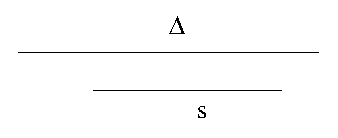
\includegraphics{templog/inclusion.eps}}}
\caption{\label{fig:inclusion} {Sequence Inclusion, $s \preceq \Delta$}}
\end{minipage}
\hfill
\begin{minipage}{6cm}
\centerline{\scalebox{0.7}{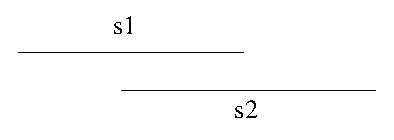
\includegraphics{templog/ordering.eps}}}
\caption{\label{fig:ordering} {Sequence Ordering, $s1 \lessdot s2$}}
\end{minipage}
\end{figure}

\begin{definition}[Sequence]\label{tl_def:sequence}
\begin{rm}
$s$ is a sequence of relations within a temporal relation sequence
$\Delta$ {\em iff} $\forall r_i \in s$ we have $\neg \exists r_l \in \Delta$ such that $r_j \le r_l \le r_k$ and
$r_j,r_k \in s$ but $r_l \not\in s$. $\quad\Box$
\end{rm}
\end{definition}

Definition~\ref{tl_def:sequence} enforces that all sequences are
continuous. 

\index{inclusion operator}
\begin{definition}[The inclusion operator, $\preceq$]\label{tl_def:inclusion}
\begin{rm}
$s \preceq \Delta$ {\em iff} $\forall r_i \in s$ we have $r_i \in \Delta$
and $s$ is a sequence in $\Delta$. $\quad\Box$
\end{rm}
\end{definition}

$s \preceq \Delta$ implies that $s$ is a subsequence of $\Delta$ and
that $s$ contains a series of consecutive states, as illustrated in~\ref{fig:inclusion}.

\index{Temporal Ordering operator}
\begin{definition}[The Temporal Ordering operators, $\lessdot$ and $\gtrdot$]
\begin{rm}
$s_1 \lessdot s_2$ {\em iff} $\quad \exists r_j \in s_1$ such that $\forall r_k
\in s_2$ we have $j < k$ and $\exists r_p \in s_2$ such that $\forall r_m
\in s_1$ we have $p > m$ and $s_1,s_2$ are sequences. $\gtrdot$ is
defined similarly. $\quad\Box$ 
\end{rm}
\end{definition}

The intuition behind our temporal ordering operator is that a sequence
comes before another sequence if at least one point in the sequence
$s_1$ is
before any in $s_2$ and $s_2$ has at least one point after $s_1$. As
desired, a subsequence of another sequence does not satisfy this
relation. Figure~\ref{fig:ordering} shows an example of sequence
ordering with an overlap between sequences.


The set of formulae of NDLTL is the
least set generated by:
\begin{enumerate}
\item Each ND $X \to^{{k}^\ast} Y$ or $X \to^{\updownarrow
{k}^\ast} Y$ is an atomic formula where ${k}^\ast \in \{ k,
\bar{{k}}, \ddot{{k}} \}$
  and $\updownarrow  \in \{ \uparrow,
\downarrow, \uparrow_r,\downarrow_r,\uparrow_d,\downarrow_d \}$.
\item If $\sigma_1$ and $\sigma_2$ are formulae then so are $\neg \sigma_1,
\sigma_1 \wedge \sigma_2, \sigma_1 \wedge^k \sigma_2$ (\mbox{k is a
constant}) and $\sigma_1 \leadsto \sigma_2$. 
\item If $\sigma$ is a formula then so are $\bm^m \sigma$ and  \diam$^m$ 
$\sigma$.
\end{enumerate}

We now define the semantics of our logic inductively.

\subsection{Semantics}\label{subsec:tl_semantics}
\index{Numerical Dependency!Semantics}
Relation state formulae are not concerned with the sequence size
used. They are obtained by performing operations on the complete
temporal relation sequence, $\Delta$. These operations represented the
ND holding at a particular state, the moving average value for a
window size $w$, or the differenced value for a particular state. We
write ($\Delta$, $u$) $\models^w$ $\sigma$ to mean that $\sigma$ holds
with respect to a window size $w$ in sequence (or state) $u$ of the
temporal relation sequence $\Delta$. We may omit $w$ if it is not
pertinent to $\sigma$; for example, $\sigma$ may be an ND alone and
$u$ may be a single relation state. The discussion of
Section~\ref{sec:tl_tsa} motivated the need for differencing. Second
order differencing, not directly expressible in our logic, is
occasionally required; an additional axiom could be added similar to
our differencing formulae.


\subsubsection{Relation State Formulae:}
\begin{enumerate}

%% STANDARD ND RULE
\item\label{item:nd} ($\Delta$, $r_j$) $\models^w$ ($X
\to^{k} Y$) { \em iff } $r_{j}$ $\models X \to^{k} Y$.

%% MOVING AVERAGE RULE
\item\label{item:ma} ($\Delta$, $r_j$) $\models^w$ ($X
\to^{\bar{{k}}} Y$) { \em iff } $r_{j-m}$
$\models X \to^{{k}_1} Y$,  $r_{j-(m-1)}$
$\models X \to^{{k}_2} Y$, $\ldots$,  $r_{j}$
$\models X \to^{{k}_{m+1}} Y$,  $r_{j+1}$ 
$\models X \to^{{k}_{m+2}} Y$, $\ldots$,  $r_{j+m}$
$\models X \to^{{k}_n} Y$ where $m = \frac{w-1}{2}$, $w$ is odd
and $\bar{{k}} = \frac{1}{w} \sum_{i = 1}^{w} {k}_i$
and $j - m \ge 0$ and $j + m \le 0$.

\item\label{item:diff} ($\Delta$, $r_j$) $\models^w$ ($X 
{\to}^{\ddot{{k}}}  Y$) { \em iff } $j > 0$ and $r_{j-1}$
$\models X \to^{{k}_1} Y$ and  $r_{j}$
$\models X \to^{{k}_2} Y$ with $\ddot{{k}} = {{k}_1} -{{k}_2}$.


\end{enumerate}

Definition 2 provides the moving average value for a {\em window} of size
$w$ for the branching
factors of the NDs for relation state $j$. At times we omit $w$ from the
following definitions for clarity. Definition 3 above provides a
difference ND values, from which a differenced sequence may be created.

All the following time
series functions used are defined in Section~\ref{subsec:tl_tsadefs}.

Relation subsequence trend formulae are required to represent trends
within our logic. These may be strict, linearly regressed, or
discordant trends. Informally, a $\uparrow$ denotes an upward trend
and $\downarrow$ a downarrow trend. We may subscript these with either
a $d$ or an $r$ to represent discordance or regression, respectively. 
In the following formulae we abbreviate {\em such that} to $s.t.$ and
denote the first relation $r_i$ in a sequence $s$ by $fst(s)$. We also
refer to a particular ND $X \to^k Y$ sequence in 
$s$ as $s_{XY}$ where necessary.

\subsubsection{Relation Subsequence Trend Formulae:}

\begin{enumerate}
%% UPWARD TREND OF MOVING AVERAGES

\item\label{item:ma_inc}($\Delta$, $s$) $\models^w$ ($X
\to^{\uparrow\bar{k}_1} Y$) { \em iff } $\mid s \mid \ge 2$ and $ \forall r_{j},r_{j+1} \in
s$ ($\Delta$, $r_j$) 
$\models^w X \to^{\bar{k}_1} Y$ and ($\Delta$, $r_{j+1}$) 
$\models^w X \to^{\bar{k}_2} Y$ for some $\bar{k}_2$, where $\bar{k}_1 \le
\bar{k}_2$.

%% DOWNWARD TREND OF MOVING AVERAGES


\item\label{item:ma_dec}($\Delta$, $s$) $\models^w$ ($X
\to^{\downarrow\bar{k}_1} Y$) { \em iff } $\mid s \mid \ge 2$ and $ \forall r_{j},r_{j+1} \in
s$ ($\Delta$, $r_j$) 
$\models^w X \to^{\bar{k}_1} Y$ and ($\Delta$, $r_{j+1}$) 
$\models^w X \to^{\bar{k}_2} Y$  for some $\bar{k}_2$, where $\bar{k}_1 \ge
\bar{k}_2$.  

%% UPWARD REGRESSION TREND 

\item\label{item:reg_tren_up}($\Delta$, $s$) $\models^w$ ($X
\to^{\uparrow_{r}{k}} Y$) { \em iff } $\mid s \mid \ge 2$ $s.t.$ $r_i
= fst(s)$ and 
($\Delta$, $r_i$)  $\models^w X \to^{k} Y$ and $reg(s_{XY}) > 0$.

%% DOWNWARD REGRESSION TREND 

\item\label{item:reg_tren_dn}($\Delta$, $s$) $\models^w$ ($X
\to^{\downarrow_{r}{k}} Y$) { \em iff } $\mid s \mid \ge 2$ $s.t.$
$r_i = fst(s)$ and 
($\Delta$, $r_i$)  $\models^w X \to^{k} Y$ and $reg(s_{XY}) < 0$. 

\end{enumerate}

In definitions~\ref{item:reg_tren_up} and~\ref{item:reg_tren_dn} we
can replace the trend operator $\uparrow_r$ with $\uparrow_d$ to
represent that we have obtained the trend using the discordance
method, Definition~\ref{def:disccoef}, in place of linear regression.

We now present two rules which allow for the representation of a trend
without an explicit initial value; these rules are necessary when we
may want to represent such a rule within our operator for all
sequences of a size $n$ ($\bm^n$) and the regression values may differ
between sequences though the general trend may be the same.

\begin{enumerate}
%% UPWARD TREND 

\item\label{item:tren_up}($\Delta$, $s$) $\models^w$ ($X
\to^{\uparrow_r} Y$) { \em iff } $\mid s \mid \ge 2$ $s.t.$
 $reg(s_{XY}) > 0$.

%% DOWNWARD TREND 

\item\label{item:tren_dn}($\Delta$, $s$) $\models^w$ ($X
\to^{\downarrow_r} Y$) { \em iff } $\mid s \mid \ge 2$ $s.t.$
 $reg(s_{XY}) < 0$.

\end{enumerate}


Relation Subsequence Formulae are required to represent the more
complex relationships within our temporal database. $\sigma$, possibly
subscripted, is either a relation state formulae or a relation
subsequence trend formulae and $s$ may be a relation state or
sequence. We note that $\wedge$ may be superscripted by $k$; this
denotes a fixed value maximum lag cross-correlation for the sequence
between $\sigma_1$ and $\sigma_2$. If $\sigma_1$ and $\sigma_2$ relate
to the same sequence then this becomes auto-correlation; we do not
consider this further due to autocorrelations for linear time series
following a dampening oscillatory pattern towards 0 as the lag
increases \cite{end95}. The use of autocorrelations for non-linear
time series in this logic is deserving of further study. $\bm^n$ is a
universal operator for all sequences of size $n$ and \diam$^n$ is its
existential dual. The final operator is $\leadsto$ which introduces a
temporal ordering between two sequences allowing for change in a
temporal database to be depicted; we shall see in
Section~\ref{sec:tl_properties} how these operators are used to form
temporal properties. We require in the following definitions that all
sequences are maximal.

\subsubsection{Relation Subsequence Formulae:}

\begin{enumerate}

%% NEG  

\item ($\Delta$, $s$) $\models \neg  \sigma_1$ {
\em iff } ($\Delta$, $s$) $\not\models \sigma_1$.


%% STANDARD CONJUNCTION

\item ($\Delta$, $s$) $\models \sigma_1 \wedge \sigma_2$ { \em iff }
($\Delta$,$s$) 
$\models \sigma_1$ and ($\Delta$,$s$) $\models \sigma_2$.


%% CORRELATED CONJUNCTION

\item ($\Delta$, $s$) $\models \sigma_1 \wedge^k \sigma_2$ { \em iff }
($\Delta$,$s$) 
$\models \sigma_1$ and ($\Delta$,$s$) $\models \sigma_2$ and $k$ is
the lag value for which the cross-correlation is maximum.

%% LEADSTO 

\item\label{item:leadsto} ($\Delta$, $s$) $\models \sigma_1 \leadsto \sigma_2$ { \em iff } ($s$,$s_1$)
$\models \sigma_1$ and ($s$,$s_2$) $\models \sigma_2$ for some $s_1,s_2 \preceq 
s$ where $s_1 \lessdot s_2$.



%% ALL FIXED SUBSEQUENCE SIZES

\item\label{item:fixed} ($\Delta$, $s$) $\models \bm^n \sigma_1$ { \em
iff }
$\forall s_i \preceq  s$ where $\mid s_i \mid = n$ and ($s$, $s_i$) $\models \sigma_1$.



%% SOME FUTURE POINT

\item\label{item:guarantee} ($\Delta$, $s$) $\models$ \diam$^n$
$\sigma_1$ { \em iff }
$\exists s_i \preceq s$ where $\mid s_i \mid = n$ such that ($s$,
$s_i$) $\models \sigma_1$.

\end{enumerate}

We note in rule (\ref{item:leadsto}) that $s_1,s_2 \preceq 
s$ do not have to cover every point in $s$.
Within this logic it is possible to express formulae such as
($\Delta$, $s$) $\models$ \safe{n} ($\sigma_1
\to$ $\sigma_2$), stating that for all $n$ size subsequences of $s$
either $\sigma_1$ does not hold or $\sigma_2$ holds.
We restrict our knowledge discovery process to
search for positive information though a user might ask such queries.

\subsection{Examples}

We now provide some examples of the logic. From
Section~\ref{subsec:tl_tsa_nd} we introduced an example of NDs in a relation
of student records. We assume that for the ND $C \to^k S$ we have 7
years of records and the relation sequence of ND branching factors is
$\Delta_{cs}$ = $\{$ 3,4,5,6,5,4,7 $\}$ where each refers to a
relation starting from 
position 0. We now highlight some rules satisfied by this sequence:

\begin{enumerate}
\item\label{ex:1} ($\Delta_{cs}$,$r_3$) $\models^3$ (C $\to^{\bar{5.33}}$ S)
\item\label{ex:2} ($\Delta_{cs}$,$r_1$) $\models^3$ (C $\to^{\ddot{1}}$ S)
\item\label{ex:3} ($\Delta_{cs}$,$s_3$) $\models^3$ (C
$\to^{\downarrow{6}}$ S) where $s_3$ = $\{ 6,5,4 \}$.
\item\label{ex:4} ($\Delta_{cs}$) $\models^3$ (C $\to^{\uparrow_r{3}}$ S)
\item\label{ex:5} ($\Delta_{cs}$) $\models^3$ $\bm^4$ \diam$^3$ (C
$\to^{\uparrow_r}$ S)
\end{enumerate}

Examples~\ref{ex:1} and~\ref{ex:2} show moving average and differenced
values for NDs. In the data mining process we generally do not need to
represent these values directly though occasionally it may be
required. Example~\ref{ex:3} provides a strict downward trend rule
within a given subsequence of $\Delta_{cs}$ and Example~\ref{ex:4}
provides similar for a linear regression trend on the
sequence. Example~\ref{ex:5} states that all sequences of size 4
contain, at some point, a sequence of size 3 for which there exists an
upward linear regression. We do not represent the exact value as these
differ within sequences but our logic allows for this, highlighted in Section~\ref{subsec:tl_semantics}. This is needed
given that general properties might 
exist, as in~\ref{ex:5}, but the exact values will differ.

\subsection{Axioms of the logic}\label{subsec:tl_axioms}
\index{Numerical Dependency LTL!Axioms}

We now highlight some additional axioms of our logic, related to
sequences, with A and B as formulae of our logic. We use $\Rightarrow$
to denote {\em implies}.

\begin{enumerate}
\item\label{ax:1} $\mbox{\diam}^n \sigma \equiv \neg \bm^n \neg \sigma$
\item\label{ax:2} $\bm^n$ A $\Rightarrow$ \diam$^n$ A
\item\label{ax:3} $\bm^n$ (A $\wedge$ B) $\equiv$ $\bm^n$ A $\wedge$ $\bm^n$ B
\item\label{ax:4} \diam$^n$ (A $\vee$ B) $\equiv$ \diam$^n$ A $\vee$ \diam$^n$ B
\item\label{ax:5} $\bm^n$ (A $\leadsto$ B) $\Rightarrow$ $\bm^n$
(\diam$^{n_1}$ A $\wedge$ \diam$^{n_2}$ B) where $n_1, n_2 \le n$
\item\label{ax:7} $\bm^m$ $\bm^n$ implies that $m \ge n$
\item\label{ax:8} \diam$^m$ \diam$^n$ implies that $m \ge n$
\item\label{ax:9} \resp{m}{n} implies that $m \ge n$
\item\label{ax:10} \pers{m}{n} implies that $m \ge n$
\end{enumerate}

Axiom~\ref{ax:1} implies that we merely have to define either $\bm^n$
or \diam$^n$ as primitive. Axioms~\ref{ax:1},~\ref{ax:2}, ~\ref{ax:3},
and~\ref{ax:4} are all properties of standard temporal
logic. Axiom~\ref{ax:5} expresses behaviour concerning
the $\leadsto$ operator. Its proof is clear from the definitions of
$\leadsto$ and $\lessdot$. Finally, axioms~\ref{ax:7},~\ref{ax:8}, ~\ref{ax:9} and~\ref{ax:10}
present some properties related to the sequence size requirements of our modal
operators.  

\medskip

Some standard axioms of temporal logic do not hold within our
logic. These include \linebreak $\bm^{m} \sigma \Rightarrow \sigma$. All
subsequences of size $m$ satisfying $\sigma$ does not imply that
$\sigma$ holds. This is due to the incorporation of statistical
functions which may hold in all sequences of a particular size but not
for the sequence as a whole. If we consider a time series there may be
a general upward trend within it though this may consist of many
local peaks and troughs; our sequence logic is capable of detecting
these. $\bm^m$ A $\Rightarrow$ \diam$^n$ A, where $m \not= n$, does
not generally hold for the same reason.

\subsection{Querying our Logic}\label{subsec:logic_query}
\index{Numerical Dependency LTL!Querying}

We now show by induction that any formulae $\sigma$ in the logic can be tested
in polynomial time. Firstly, we present some lemmas which shall be of use
in the proof.


\begin{lemma}\label{lemma:subseq}
\begin{rm}
Given a sequence $s$ of $n$ relation states then $s$ has $\frac{1}{2}
n(n+1)$ subsequences
\end{rm}
\end{lemma}

{\em Proof.} There are $n$ subsequences of size 1, $n-1$ of size 2,
$\ldots$, 1 of size $n$. $n + (n-1) + (n-2) + \ldots + 1$ = $\frac{n(n+1)}{2}$. $\Box$

We note that a sequence of size 1 contains two relations, temporally
ordered. 
\begin{lemma}\label{lemma:seq_initiate}
\begin{rm}
The number of subsequences which start in position $k$ in
a sequence of size $n$ is $n-k$. We assume the first position is
denoted by 0.
\end{rm}
\end{lemma}

{\em Proof.} Trivial. $\Box$


\begin{figure}[ht]
\centerline{\scalebox{0.6}{\includegraphics{../Event_theory/sequence.eps}}}
\caption{\label{fig:sequence} All possible subsequences in a sequence
containing 7 relations}
\end{figure}


\begin{lemma}\label{lemma:seq_extend}
\begin{rm}
Assuming a total sequence length $m$ and a sequence $s$ which begins
in position $k$ of the complete sequence. The number of sequences
which start after and end after a sequence $s$ of size $n$ is:  
\[
\sum_{i = k+1}^{m} m - i - \sum_{i = 1}^{n-1} n - 1
\]
\end{rm}
\end{lemma}

{\em Proof.} Clear, using the facts that we wish to count all
sequences which start at position \linebreak $k+1$ onwards to the end of the
sequence which sums lemma~\ref{lemma:seq_initiate} and we wish to
exclude those subsequences from position $k + 1$ which do not end
after $s$, therefore we remove all subsequences contained at each
position from $k+1$ to $k+n$ that are contained in a sequence of size
$n-1$. $\Box$  
 
\begin{theorem}\label{theorem:pt_logic}
\begin{rm}
Given a subsequence $s$ of a relation sequence $\Delta$ and a formulae $\sigma$ in NDLTL
we prove that ($\Delta$, $s$) $\models \sigma$ can be shown in
 polynomial time.
\end{rm}
\end{theorem}

\smallskip

{\em Proof.} We show inductively that we can test if  
($\Delta$, $s$) $\models \sigma$ in
polynomial time. We base our proof on the structure of $\sigma$.

\smallskip
({\em Basis}): If $\sigma$ is an atomic formula of the form $X
\to^{\uparrow{k}} Y$ or  $X \to^{\downarrow{k}} Y$ we
examine each consecutive pair of points (relations) in $s$ to determine if the trend
is satisfied. This can be achieved in linear time. Similarly we can
test branching factor values of regression and discordance in linear
and polynomial time respectively.

\smallskip
({\em Induction}): We now consider all possible structures of
$\sigma$. If $\sigma$ is of the form:
\begin{enumerate}
\item $\neg \sigma$  we need to determine if ($\Delta$, $s$)
$\not\models \sigma$. We assume, by the inductive hypothesis, that
$\sigma$ can be checked in polynomial time. Therefore it is easy to
see that $\neg \sigma$ can also be checked by polynomial time.
\item $\sigma_1 \wedge^k \sigma_2$ - we assume that $\sigma_1$ and
$\sigma_2$ can be determined in polynomial time and it is clear that
the result of the cross-correlation function
ccor(br($\sigma_1$),br($\sigma_2$),k) can be computed in polynomial
time. Similarly $\sigma_1 \wedge \sigma_2$ holds.
\item $\sigma_1 \leadsto \sigma_2$ can be tested in time polynomial
from lemma~\ref{lemma:seq_extend}.  
\item \safe{n} $\sigma$ can be determined if for all subsequences of $s$
we can show that $\sigma$ holds.  Given \safe{n} there
are $\frac{n(n+1)}{2}$ subsequences of $s$ where $n$ is at most the
size of the sequence. We assume that each
subsequence can be checked in time polynomial, implying that \safe{n}
$\sigma$ can be checked in polynomial time.
\item \guar{n} $\sigma$ holds if there is at least one subsequence
$s_2$, of size $n$,
of $s$ such that ($s, s_2$) $\models \sigma_1$ and it is clear
that we can examine each subsequence of this individually in
polynomial time.
\end{enumerate}
We have shown by induction on the structure of $\sigma_1$ that we can
check if this is satisfied in polynomial time. $\quad\Box$
 

We now show why we restrict ourselves to sequences of a fixed
length. We define a {\em cover} to be a set of sequences of different
sizes whose union contain the complete sequence. In a time series
there may be properties which hold across different sequence sizes,
however we now show that there is an exponential number of such {\em
covers}.  

\begin{lemma}\label{lemma:covernum}
\begin{rm}
Given a sequence $s_n$ containing $n$ relation states then $s_n$ has
$\frac{(n+1)!}{2}$ covers, where $n!$ denotes $n$ factorial.
\end{rm}
\end{lemma}

{\em Proof.} If there is 1 relation in a sequence there is only 1
cover.  If $n > 1$
then we state that there are $m_n$ covers.  We note that an $n-1$ size
sequence has $m_{n-1}$ covers. A sequence $s_n$ will have one more
relation in the sequence than $s_{n-1}$. The additional relation state in
$s_n$ provides an additional $n+1$ ways of combining with $m_{n-1}$ so
we have the recurrence relation
\begin{eqnarray*}
	m_1	& = & 1 \\
	m_n	& = & (n+1)m_{n-1}
\end{eqnarray*}
We can easily see that $m_n = (n+1)(n)(n-1)(n-2) \ldots 3.1$
which is equivalent to $\frac{(n+1)!}{2}$  $\Box$

\medskip

We therefore restrict ourselves to fixed length sequences in the logic
for safety properties ($\bm^n$) defined in Section~\ref{sec:tl_properties}.

\subsection{Expressiveness of NDLTL}
\index{Numerical Dependency LTL!Expressiveness}

We wish to know how expressive are the temporal connectives of our
logic? In propositional temporal logic we know that the connectives
{\em since}, ${\cal S}$, and
{\em until}, ${\cal U}$, are defined as fully expressive by \cite{gps80}
due to their satisfaction of 
the separation property, where any formulae can be rewritten as a
combination of past, present, and future, over integer time. 
The only temporal operator
our logic permits is $\leadsto$, due to $\bm^n$ and \diam$^n$ relating
to sequences. We are only interested in certain
temporal orderings within sequences and we know that use of ${\cal
U}$, or other temporal operators, 
might frequently be too restrictive; the changing nature of ND values
in a temporal relation sequence and in a temporal database may require
many instances of ${\cal U}$.
We consider the expressiveness of
our logic with respect to time series as the capability of expressing
patterns. 

\medskip
We consider the following for pattern expression with respect to
linear regression, without loss of generality. Within any single time
series and for a sufficient sequence size we can express patterns in a
time series obtained using linear regression and using the connective
$\leadsto$. At the finest
granularity these sequences may contain only two points. If we
consider multiple 
time series the sequence size must be fine enough for representation
of change in any of the patterns in any of the time series. Our
temporal operator $\leadsto$ is not expressively complete as we can
not state sentences of the form 'A before B'. It is reasonable to view
the restriction to fixed length sequences as necessary for uniform
property discovery, given the result of
lemma~\ref{lemma:covernum}. Any sequence of size $n$ can be separated
into 
subsequences of any fixed size $m$, where $m \le n$, which enhances
the expressive nature of the logic. Due to lemma~\ref{lemma:covernum}
it is not feasible to consider otherwise within an applied scenario.

\medskip

When we move into time
series issues of expressive completeness become vague as we do not
know what is complete when denoting the relationship between two or
more time series. The
temporal and modal connectives of our logic are clearly incomplete and
require further study; we have
formulated them such they are sufficient for the data mining task at hand.


\section{Temporal Logic Properties}\label{sec:tl_properties}
\index{Temporal Logic Properties}
\index{Temporal Properties|see{Temporal Logic Properties}}


We now show how we can use our logic for the expression of properties
which may hold for a temporal sequence. Initially, we informally
discuss the intuition behind the properties holding in our logic and
provide a brief survey of the field.
\medskip

\cite{pnu77} introduced the application of temporal logic for program
verification. \cite{gps80} presented numerous {\em properties} for the
application of temporal logic to reactive and concurrent
(non-terminating) programs. Such programs could not utilise previously
developed correctness methods given that these methods were intended 
for finite (terminating) programs. Much of the literature refers to
the two general forms of properties, {\em safety } and {\em
liveness}. Safety properties refer to the intuition that ``nothing
bad ever happens'' whilst liveness properties imply that ``something good
eventually happens'' \cite{sis94}. We can see in program verification how we
might want to prevent particular conditions from ever being satisfied
(safety) whilst at the same time ensuring that specific condition are
satisfied intermittently (liveness). From these definitions we can
infer the dual universal and existential natures of safety and
liveness. These are also referred to as the two most general classes
of invariances and eventualities.

\medskip

We now provide two brief examples of safety and liveness properties
from program verification \cite{eme90}. If we assume that $s$ and $h$
are the initial and final labels of a program then $s \wedge \phi
\Rightarrow \Box (h \Rightarrow \psi)$, where $\Rightarrow$ denotes
implication, is a safety property. It infers that if a program in state
$s$ satisfies $\phi$ then at all points in the future the final state
implies $\psi$. We view $\phi$ and $\psi$ as pre- and
post-conditions. Mutual exclusion and deadlock prevention principles are
also examples of safety properties.  Liveness properties consist of
intermittent assertion, total correctness and guaranteed accessibility
conditions. To illustrate, $s \wedge \phi \Rightarrow \Diamond (h
\wedge \psi)$ is the total correctness property implying that a
program starting in $s$ satisfying $\phi$ will, at some point in the
future, halt in  $h$ satisfying $\psi$. We can see from these simple
examples how temporal logic is directly applicable for program
verification. Proof theoretic methods for program verification, not
considered here, have been developed and the most appropriate proof
method depends on the property being verified.

\medskip
\index{Safety Property}
\index{Guarantee Property}
\index{Temporal Logic Properties!Safety}
\index{Temporal Logic Properties!Guarantee}

Properties may take numerous forms which we now outline.
Safety properties have the canonical form \safe{n} $\sigma$. We may
refer to invariant NDs as safety properties. The ``informal''
description of safety, stating that nothing bad ever happens implies
that it is a bad thing if $\sigma$ does not hold in a
relation. \cite{sis94} describes {\em strong safety} properties which
remain safety properties after the exclusion of a state. In our logic
all possible sequences satisfying a property imply that it is a safety
property.  For example ($\Delta$,$s$) $\models$ \safe{n} $(X \to^{\up
k} Y)$ implies that all 
subsequences of $s$ satisfy an upward trend from value $k$.
Conditional safety properties have the form $\sigma_1$ $\leadsto$
\safe{n} $\sigma_2$. We
can refer to this as a {\em trigger}, denoting that once $\sigma_1$
occurs then at some point after $\sigma_2$ will hold in all sequences
of size $n$. It is apt within a finite
temporal sequence wherein a certain value may imply other values for all
subsequent states.

%% CONDITIONAL GUARANTEE
\medskip
Guarantee properties have the canonical form \guar{n} $\sigma$.
A conditional guarantee property implies that all subsequences of
a fixed size $n$ 
always contain a sequence where $s_1 \lessdot s_2$ and
($\Delta$,$s_1$) $\models$ \diam$^{m}$ $\sigma_0$ which leads to 
($\Delta$,$s_2$) $\models$ \diam$^{m}$ $\sigma_1$. This is written as
($\Delta$,$s$) $\models$ \safe{n} ( $\sigma_0 \leadsto$ \diam$^{m}$
$\sigma_1$) where $s_1,s_2 \preceq s$.

\medskip

Obligation properties are the disjunction of canonical safety
and guarantee properties \guar{n} $\sigma_1$ $\vee$ \safe{m}
$\sigma_2$. A canonical
obligation formula is a conjunction of these properties. Note that the
sequence sizes need not be the same, though the semantics of this in a
knowledge discovery context is not clear.

\smallskip
\index{Response Property}
\index{Temporal Logic Properties!Response}
Response properties are of the general form \resp{n}{m} $\sigma$. A
Canonical response property can also be viewed as a seasonal 
occurrence property and is represented by 
($\Delta$,$s$) $\models$ \resp{n}{m} $\sigma$. Within sequence $s$ all
sequences of size $n$ contain an occurrence of $\sigma$ which will hold at some point  in the
$s$. The temporal logic definition states that at a particular point
all points imply that $\sigma$ will hold at some point in the
future. Our definition is that  
all sequences of size $n$ will, at some point, contain a sequence of 
size $m$ which satisfies $\sigma$. It is clear that we can use this
property to present seasonal behaviour to the system user.
Alternatives for standard temporal logic, listed in \cite{mp92}, are
$p \to \Diamond q$, 
known as response to an impulse, and
$\Box(p \to \Diamond q)$ where $\Diamond$ implies at some point in the
future and $\Box$ implies at all points in the future.
Within our logic a response property may occur only finitely
many times. A seasonal response property implies a regular chain of
two, or more, events written as
($\Delta$,$s$) $\models$ \resp{n}{m} ( $\sigma_0 \leadsto \sigma_1$
). An immediate response property in temporal logic states that at a
particular point 
all points imply that $\sigma$ will hold at the next point, written as
$\Box \bigcirc \sigma$. We do not incorporate this within our logic of
sequences given that the representation of the {\em next} sequence
will often, depending on sequence size, contain a significant overlap
which would frequently result in the discovery of uninteresting properties.

\medskip
\index{Persistence Property}
\index{Temporal Logic Properties!Persistence}

Persistence properties in standard temporal logic, written as
$\Diamond\Box p$, may be triggered by a preceding
event where we infer that all positions from a certain time on
satisfy $p$. This directly translates to our logic where we
write persistence as
($\Delta$,$s$) $\models$ 
\pers{n}{m} $\sigma$. In our sequence logic a
persistence property implies that at some point in a sequence $s$ of size
$n$ all sequences within $s$ of size $m$ satisfy $\sigma$. This allows
us to depict properties which may hold in nonlinear time
series, for example, a continuous downward trend in an otherwise
rising microchip stock
due to an unforeseeable influence, such as fires in the chip factory
destroying stock. It is likely that this would otherwise represent
nonlinear behaviour. Ordered persistence properties, written as 
($\Delta$,$s$) $\models \sigma_0 \leadsto$ \pers{n}{m} $\sigma_1$ are
not directly relevant in our work due to a single occurrence of
$\sigma_0$ possibly having no relation to \pers{n}{m} $\sigma_1$.

\medskip

Reactive properties, shown in \cite{mp92} to be the maximal
class of properties which needs to be considered, are written as
\resp{n}{m} $\sigma_1$ $\vee$ \pers{p}{q} $\sigma_2$. Within the
finite sequence of our logic and the knowledge discovery process such
a property found would represent complex behaviour. Such a reactive
property might denote the oscillation between $\sigma_1$ occurring
sporadically in all $n$ size sequences and $\sigma_2$ holding
continually within all $q$ size sequences within a sequence of size
$p$. This may represent a relationship between $\sigma_1$ and
$\sigma_2$. The reactive formulae could also be restricted just to
contain the same atom in each disjunct, which may be more interesting.


\subsection{Application of Properties}
\index{Temporal Logic Properties!Application}

We now show how the properties are related to each other and extend
the discussion to include data mining applications. We note that
the classification provided in Figure~\ref{fig:Classification}, given
in \cite{mp92}, for temporal logic properties holds within our logic,
exemplified by the axioms of Section~\ref{subsec:tl_axioms}. We make
use of this {\em hierarchy} to discover rules in an incremental fashion.

\begin{figure}[ht]
\centerline{\scalebox{0.8}{\includegraphics{../Event_theory/Prop_class.eps}}}
\caption{\label{fig:Classification} A Classification of Temporal
Properties}
\end{figure}
\index{Temporal Logic Properties!Classification}
The classification of temporal properties aids the process of
knowledge discovery as we move concurrently from smaller to larger
sequences and from obtaining different properties according to their
classification in the hierarchy. The structure of properties, which we
believe to contain a good classification of interesting patterns,
therefore simplifies the data 
mining process. The value of these properties in program verification
translates directly to knowledge discovery. We discuss this further in
Chapter~\ref{chap:tempresult}.  

\section{Discussion}\label{sec:tl_disc}


Our logic conveys information within time series without the need to
compare or analyse specific values, unlike a standard statistical
analysis. Moreover, on top of this analysis we seek to discover
properties, derived from those used within program verification, which
the time series satisfies. Representation in our
symbolic logic itself enhances the overall knowledge discovery
process. \cite{hr83} present a belief logic for reasoning about the
likelihood of events with a modal operator ${\cal L}$ to state that an
event is likely to happen.  The application of this logic is as a
decision support tool where, the authors claim, a statement ``it is
likely that s'' is more useful than saying ``s will occur with
probability 0.63.'' Numbers may be attached to the modal operator
${\cal L}$ to provide a degree of likelihood. Similarly, our logic may
be viewed as a decision support tool when we state that, for example,
in all monthly periods the trends in a particular bank lead the trends
in its insurance subsidiary by one day. This formula expressed
succinctly will directly aid any decision support process. Also,
symbolic rules provide more information support than a graphical
analysis as well as expressing data in a machine understandable form
which is transferable to other knowledge discovery tools.

\medskip

Further work is required to study the expressive nature of our logic
which may lead to enhancements within the data mining process for
knowledge discovery. Two mechanisms suggest themselves: (1) to include
additional temporal operators within sequences, and (2) to extend the
time series functionality of the logic at the atomic (and possibly at
the connective) level. The latter could easily be extended to use
techniques from related research, such as the discrete Fourier
transform \cite{alss95,dgm97,raf99}, upon which we then search for properties.

\medskip

We examine how our logic for NDs can be applied for
inferring additional dependencies within a temporal relation sequence.
If this logic were restricted further to FDs
alone
then the axioms of reflexivity, augmentation and transitivity are
invariant within this language. For example, using $\Rightarrow$ to denote
{\em implies}, we have, with respect to a sequence, 
$\bm^n X \to Y \Rightarrow \bm^n XZ \to YZ$ where $X,Y,Z \subseteq R$. Inference
within the language is also similar to standard FD inference: 
\begin{displaymath}
\bm^n (A \to B) \wedge \mbox{\diam}^n (B \to C) \Rightarrow
\mbox{\diam}^n (A \to C) 
\end{displaymath} or
\begin{displaymath}
\bm^n (A \to B) \wedge \bm^n ((A \to C) \vee (B \to C)) \Rightarrow
\bm^n ((A \to C)) 
\end{displaymath}

A logic with FDs as atomic formulae provides much more flexibility
that incorporating Boolean dependencies into the model \cite{drs93}
given that we have the enhanced expressiveness of temporal
operators. This is a possible avenue for further research.
 
\medskip

Within a temporal query language we propose that it would be valuable
to be able to form queries asking if certain properties are satisfied over
a given time period. These properties could be defined with respect to our, or
another, logic. They also need not exactly conform to ND sets. Their
use would be widespread both in data mining and for integrity
analysis. For example, in a financial data mining system a user might
want to ask if a persistence property holds in some yearly period for
all monthly segments.  A positive result might imply some seasonal
behaviour that would not have been directly deducible from a visual
analysis. 


\medskip

Schema evolution \cite{rod94} is a research area on the fringes of
temporal data mining. Schema evolution is defined as the ability for a
database schema to evolve without the loss of existing
information. Mining the changes in schemas for patterns is a valid
temporal data mining research area, not yet well developed.
\cite{van93} presents an interesting discussion of evolutionary schema
mutation and the converse of these ideas can be adopted for data
mining. The methodology presented herein could mine
different segments of temporal databases for properties; a comparison
for properties found could then be conducted on relation sequences
having different schemas. For example, an attribute $sterling\_value$
may be updated to $ecu\_value$; this may or may not affect the general form
of knowledge discovered.  


\medskip
















































































































































































































































































































\chapter{Temporal Property Detection with Numerical Dependencies and
Resampling}\label{chap:tempresult}

We now present results of our temporal logic for knowledge discovery
from NDs in temporal sequences applied to
real world data. In Section~\ref{sec:tr_intro} we discuss  the context
of our experiments and present the model for the discovery of
properties in Section~\ref{sec:tr_propmodel}. The model we provide,
given the flexibility of our logic, is not rigid and numerous
algorithms may be created to extend or diverge from this model. 
We present one algorithm in this context, noting that other algorithms
are direct implementations of the semantics provided by the logic. 
The results of our
experiments are presented in two sections. Firstly,
in~\ref{sec:tr_relseq} we present results gained from temporal
relation sequences satisfying NDs. Then, in
Section~\ref{sec:tr_tsares} we discuss results from experiments on
standard time series data obtained from financial stocks. We present
an analysis of our work in the context of this research area in
Sections~\ref{sec:tr_case1} and~\ref{sec:tr_case2}, as two case
studies, relating these 
results to behaviour in 
the real-world in Section~\ref{sec:tr_real_analysis}. In
section~\ref{sec:mbb_large} we introduce the moving blocks bootstrap
for large relations and provide a
critical study of our methodology in~\ref{sec:tr_crit_an}. We compare
our work with other work conducted on time series similarity in
Section~\ref{sec:tr_sim_ass}. We conclude in Section~\ref{sec:tr_disc}.

\section{Introduction}\label{sec:tr_intro}

The flexibility of the
logic implies that the knowledge discovery process requires
restriction of the types of rules found to prevent trivial rules being
discovered; we therefore focus on the discovery of properties, defined
in Section~\ref{sec:tl_properties}, 
for pairs of temporal datasets. The discovery of properties used
within program verification has not previously been applied to
knowledge discovery. Obviously our 
work is closely related to other work on rule discovery though our
logic allows for temporal relationships to be discovered. As we have
seen in~\ref{subsec:temp_mine}, \cite{bt98} is
a recent work which uses temporal logic for rule discovery; the logic
used is a standard temporal logic and as such requires restriction for
interesting patterns to be found. The use of properties places such a
restriction on patterns to be discovered whilst at the same time
ensures the discovery of interesting properties.

\medskip

\index{Property Discovery Model}
Our property discovery model incorporates aspects of the property
classification hierarchy thereby simplifying the knowledge discovery
process. We move from obtaining values of statistical functions at the
sequence level to the creation of safety and guarantee rules and then
to a larger sequence size for the discovery of more complex
properties, such as response and persistence.
Within the knowledge discovery process we employ moving blocks
resampling to discover short range properties. The moving blocks
bootstrap considers all possible blocks of a given size $n$ within an
input time series. A resampled time series is then formed by randomly
selecting blocks from the original series and appending each block to
the resampled series until the resample is equal to or greater than
the length of the original series.  Different time series are sampled
from simultaneously so that relationships between series are preserved
within blocks. Property discovery may then be
applied to this resampled sequence knowing that relationships have
only been preserved within blocks. We show that useful conclusions can
be found from this process, particularly in conjunction with property
discovery from the original process. Our data mining model is no
different from typical data mining systems which, as \cite{man96}
states, have modest aims in terms of the complexity of the knowledge
obtained. 
\medskip

We applied our property discovery model to a number of different data
sets including National Football League (NFL) data over 3 seasons and data
sets of US National Notifiable disease data, both of which we could
mine for ND set satisfaction. Restricting our logic solely for time
series we then applied our methods to stocks from the FTSE 100. We found
rules which complement the graphical depiction of a time series. Because we
are referring explicitly to time series and not NDs in a temporal
relation sequence we do not have specific attributes within which to refer
to trends, or similar, so we use placeholders, in this case $bp$ and $sh$.
To
illustrate, we found the following property in two oil stocks, BP ($bp$) and
SHELL ($sh$), represented as $\Delta_{oil}$ $\models^3$ \pers{30}{15} ($bp$ $\downarrow_r$ $v_1$
$\wedge^0$ $sh$ $\downarrow_r$ $v_2$) where $\downarrow_r$ implies a downward
regressive trend and $v_1,v_2$ are the initial values of the stock
when the rule holds (found at 7 locations over 242 days). 
 Graphical analysis of these stocks (in Figure~\ref{graph:bp_11mn_1})
would suggest 
a definite relationship but any general trends are obscure. This
result for these sequence
sizes suggests downward trends have lasted longer than upward from 1
December 1997 to 1 November 1998 for these stocks. Many additional results 
showed that interesting and unexpected properties were
discovered, which we detail and analyse, that both complement and
extend a graphical depiction.

\medskip

For the sake of clarity we often present rules without specific values
which we believe would not aid in the presentation or understanding of
the rule. The analysis of data mining methods is both an empirical and
theoretical science. Measures are used for the latter whilst expert
analysis is incorporated into the former. The results we find here,
given that they are expressed in a logical form, are assessed
empirically. The use of standard statistical functions within our
logic implies that all results are statistically
sound. 

\section{Property Discovery Model}\label{sec:tr_propmodel}
\index{Temporal Properties}
\index{Property Discovery Model}

We may validate our property discovery model of
Figure~\ref{fig:model2} as follows. Our model is a natural
generalisation of the upward formation of property discovery based on
the formalisation of our logic. The goal is the discovery of
properties within the framework of the temporal logic of sequences
described in Section~\ref{sec:tl_ndltl}. A standard time series
analysis would examine series for potential correlations,
cross-correlations and similar functions \cite{ko90}. The functions
would take as 
input either the original time series, or a moving average time series
to allow smoothing or a differenced time series for trend removal or a
combination of these. The first part of our model 
incorporates this behaviour linearly by creating moving averages before
searching for correlations. We also note that
we may also create resampled sequences upon which we apply moving
average and differencing techniques. After this initial step we seek
to obtain reliable trends for sequence description.

\medskip

At this stage we then have expressions representing the temporal
relation sequence. These expressions of
our logic do not contain any of the modal operators. Firstly, we may
obtain a complete sequence description by applying $\leadsto$ to the
non-modal expressions for a specific sequence size $n$. This may
optionally include the correlations between NDs in the given input
template of FDs F. 

\medskip

The final section of the property discovery model seeks to discover
properties of our logic containing the $\bm^n$ and \diam$^n$ modal
operators using the classification hierarchy of Figure~\ref
{fig:Classification}. Indicated in Figure~\ref{fig:model2} by the
upward arrows from response to guarantee properties and from
persistence to safety properties is the potential for recursive
property discovery; such as a safety property containing persistence
rules.  We could not attempt to discover properties
without first having expressions, similarly we do not wish to
discover expressions without first applying moving average,
differencing, and/or resampling techniques; it would not make sense
to, say,
create the moving average of a trend expression after we had broken it
up into sequences due to extra repeated computation and, perhaps,
different results due to increased {\em end effects}.

\begin{figure}[ht]
\centerline{\scalebox{0.7}{\includegraphics{../Event_theory/model2.eps}}}
\caption{\label{fig:model2} A description of our Temporal Property
Discovery System}
\end{figure}


We now step through the property discovery model. Input is a sequence
of $n$ relation states. 
Each relation in this sequence
satisfies a set of NDs. We wish to provide details of {\em properties}
which may hold in the sequence. From the initial relation sequence we
may form series of moving averages of windows, each of size $w$, so that
the sequences we in effect deal with are
moving average sequences, each of
size $n - (w-1)$, given the original relation sequence is of size $n$,
or we can simply use the original relation sequence for
trend detection. Differenced lists can also be created for seasonal
property detection. 
We also have the option of employing {\em jackknife}
resampling \cite{efr82}, for smoothing, at this point so that the
sequences are robust i.e. noisy outliers are weakened by the use of
resampling.  We consider examples both with and without jackknife
resampling. We can also apply the moving blocks bootstrap to recreate
time series for short range property detection.  
\medskip


Using
this information we then can gain trend, cross- and auto-correlation,
and sequence description information. We examine the sequence for correlation
and sequence description purposes all sequences of a fixed size
$n$. This allows us to find safety and guarantee properties with
regard to $n$.  We also obtain an input for a larger sequence size 
$m$ so
that complex properties, such as response properties, are detected
with respect to $m$ and $n$. Additional flexibility
is therefore achieved by looking for patterns of $n$  time points
within larger sequences $m$ time points. Property discovery occurs in
a bottom-up fashion whilst querying, if enabled, would occur top-down.

\medskip

If all sequences of a
fixed size satisfy a rule we refer to this as a {\em safety property},
whereas there may exist a set of sequences such that a property holds
throughout the complete sequence but not for subsequences of a fixed
size, which we denote as a {\em cover}, which may imply irregular
behaviour. As we have shown there are an exponential number of such
covers and we do not attempt to discover these. 
If any of these properties occur not for the complete sequence but for
a complete subsequence we
denote this by creating persistent 
properties. Figure~\ref{fig:model2} also shows that properties may themselves
contain properties, such as a safety property for persistence
rules. This would then require three sequence sizes to be given by the
user or for incremental steps in sequence size to be performed within
the discovery process. We limit ourselves to two sequence sizes.



\subsection{The Generic Property Discovery Algorithm}\label{subsec:tr_genalg}
\index{Property Discovery Model!Generic}

In the data mining literature there has been much discussion of
working towards a common framework for data mining, presenting
comparisons of data mining now to database research in the 60s before
the adoption of the relational model \cite{fps96b,man96}. Generic algorithms for data
mining have been proposed, most notably by \cite{man96},
extended in \cite{man97}. We now outline this generic procedure. A
candidate set of initial patterns is provided by the user. The
database (or data set) is then examined to see if these patterns occur
a sufficiently frequent number of times, in which case they are
classified as interesting. A new candidate set is generated from the
interesting patterns and the previous candidate set and the process is
repeated. This is continued until there are no new candidate elements
and the interesting set is returned as knowledge discovered. We can
see that our algorithm~\ref{alg:propmine} has a similar skeleton to
this generic procedure. Our procedure is general in that we consider
the satisfaction of a property to be interesting and the natural
classification of properties allows properties to be discovered using
the input relation sequence and the properties previously discovered. 
Using Figure~\ref{fig:Classification} as a basis, property set $p_1$
is higher than set $p_2$ if there does not exist a property 
in $p_2$ which is formed from a property in $p_1$. We also assume that
within sets $p_1$ or $p_2$ no properties are formed from any other
properties in the set. 
 
{\line
\begin{figure}[ht]
\begin{center}
\fbox{\begin{minipage}{16cm}
\begin{algorithm}[{\rm Property\_Mine}({\rm $\Delta$}, {\rm F})]\label{alg:propmine}
\begin{rm}
\begin{tabbing}
t1\=t2\=t3\=t4\=t5\=t6\=t7\= \kill \\
\ra.  \> \> {\bf begin} \\
\sa.  \> \> \> Rule\_set :=  $\emptyset$; \\
\sa.  \> \> \> {\bf while} $\exists$ a new classification of
properties {\bf do} \\
\sa.  \> \> \> \> {\bf for each} property $p$ at same classification $c$ {\bf do}\\
\sa.  \> \> \> \> \> Rule\_set := $\{ q \mid p$ property rule $q$
discovered from $\Delta$, F, and Rule\_set $\}$  $\cup$ Rule\_set;\\
\sa.  \> \> \> \> {\bf end for}\\
\sa.  \> \> \> \> $c$ := Next classification of temporal properties \\
\sa.  \> \> \> {\bf end while }\\
\sa.  \> \> \> {\bf return} Rule\_set; \\
\sa. \> \> {\bf end.}
\end{tabbing}
\end{rm}
\end{algorithm}
\end{minipage}}
\caption{\label{tr:fig:propmine} The Generic Property Data Mining Algorithm}
\end{center}
\end{figure}
}



\subsection{The Response Persistence Algorithm}\label{subsec:tr_resppers}
\index{Response Persistence Algorithm}


In Algorithm~\ref{alg:resp}, detailed in Figure~\ref{tr:fig:resp}, we
present a simple algorithm for detecting response and persistence
properties with respect to two sequence sizes given by the user. This
may be considered as a direct specialisation of
Algorithm~\ref{alg:propmine}. For this algorithm the classification is
$\{ \{$ Safety, Guarantee $\}$, $\{$ Response, Persistence $\} \}$.
Algorithm~\ref{alg:resp} accepts a temporal relation sequence $\Delta$
and a set of FDs F, which we assume are satisfied as NDs, together
with lower and upper sequence sizes. The algorithm works in a bottom up
fashion such that all formulae which may hold are classified into
sets of formulae for each subsequence. Membership of formulae in any
or all of these sets then determines if a rule in a higher
classification is satisfied.

{\line
\begin{figure}[ht]
\begin{center}
\fbox{\begin{minipage}{16cm}
\begin{algorithm}[{\rm Response\_Persistence}($\Delta$, {\rm F}, $n$, $m$)]\label{alg:resp}
\begin{rm}
\begin{tabbing}
t1\=t2\=t3\=t4\=t5\=t6\=t7\= \kill \\
\ra.  \> \> {\bf begin} \\
\sa.  \> \> \> Main\_Rule\_set :=  $\emptyset$; \\
\sa.  \> \> \> Final\_Rule\_set :=  $\emptyset$; \\
\sa.  \> \> \> {\bf for each} subsequence $s$ of $\Delta$ of size $m$ {\bf do}\\
\sa.  \> \> \> \> Rule\_set := $\emptyset$; \\ 
\sa.  \> \> \> \> { \bf for each} subsequence $s_n$ of $s$ of size $n$
{\bf do}\\
\sa. \> \> \> \> \> Rule\_set$_{s_n}$ := Rule set discovered for $s_n$
wrt F; \\
\sa. \> \> \> \> \> Rule\_set := $\{$ Rule\_set$_{s_n}$ $\}$ $\cup$ Rule\_set; \\
\sa.  \> \> \> \> {\bf end for}\\
\sa.  \> \> \> \> M\_rule := $\emptyset$; \\
\sa.  \> \> \> \> {\bf if } $\forall$ $r$ $\in$ Rule\_set $\exists \sigma$
 such that $\sigma \in r$ {\bf then} \\
\sa.  \> \> \> \> \> M\_rule := $\{ \bm^n \sigma \} \cup$ M\_rule; \\
\sa.  \> \> \> \> {\bf end if};\\
\sa.  \> \> \> \> {\bf if } $\exists$ $r$ $\in$ Rule\_set and $\exists$ $r_2$
$\in$ Rule\_set with $r$ $\not=$ $r_2$ \\
\> \> \> \> \> such that $\sigma \in r$ and $\sigma \not\in r_2$ {\bf then} \\
\sa.  \> \> \> \> \> M\_rule := $\{$ \diam$^n$ $\sigma \} \cup$ M\_rule;\\
\sa.  \> \> \> \> {\bf end if};\\
\sa.  \> \> \> \> Main\_Rule\_set :=  $\{$ M\_rule $\}$ $\cup$ Main\_Rule\_set; \\
\sa.  \> \> \> {\bf end for}\\
\sa.  \> \> \> {\bf if } $\forall$ $r$ $\in$ Main\_Rule\_set $\exists \sigma$
such that $\sigma \in r$ {\bf then} \\
\sa.  \> \> \> \> Final\_Rule\_set := $\{ \bm^m \sigma  \}$ $\cup$ Final\_Rule\_set; \\
\sa.  \> \> \> {\bf end if};\\
\sa.  \> \> \> {\bf if } $\exists$ $r$ $\in$ Main\_Rule\_set and $\exists$ $r_2$
$\in$ Main\_Rule\_set with $r$ $\not=$ $r_2$ \\ 
\> \> \> \> \> such that $\sigma \in r$ and $\sigma \not\in r_2$ {\bf then} \\
\sa.  \> \> \> \> Final\_Rule\_set := $\{$ \diam$^m$ $\sigma \}$ $\cup$ Final\_Rule\_set;\\
\sa.  \> \> \> {\bf end if};\\

\sa.  \> \> \> {\bf return} Final\_Rule\_set; \\
\sa. \> \> {\bf end.}
\end{tabbing}
\end{rm}
\end{algorithm}
\end{minipage}}
\caption{\label{tr:fig:resp} The Response Persistence Algorithm}
\end{center}
\end{figure}
}




\section{Relational Sequence Data Sets}\label{sec:tr_relseq}
\index{Temporal Sequence!Data Sets}

We now discuss the experiments carried out and the results achieved
using NDLTL. Given the flexibility of our logic it is easy to extend
the results presented here by: 
\begin{itemize}
\item Allowing the user to query a given input. He may want to know,
using sales data obtained daily over 2 years, if there is a peak of sales in every quarter, and
express this using our logic. This example shows a possible
seasonality query which would take the form \linebreak[4] \resp{730}{90} (X
$\to^{\uparrow_r K}$ Y $\leadsto$ X $\to^{\downarrow_r K}$ Y)
\item Modifying the time series functions within the logic. Different
functions can be incorporated, for example, that are specifically
known to handle nonlinear time series better than linear regression or
discordance.
\end{itemize}

We now present the results, initially focusing on ND temporal relation
sequences and
then moving on to time series results alone. We focus on the latter
due to the lack of significant real-world data available for temporal
data (it is easier to obtain public data, such as share closing prices,
compared to a database of employee data over the last 20 years). We
also concentrate on time series due to the availability of data with a
significant number of points, whereas a temporal database may only be
updated monthly/yearly, though this is changing for many automated
knowledge discovery and data warehousing applications.


\subsection{Results}\label{subsec:tr_relres}
\index{Property Discovery Model!Results}

We present two datasets used to obtain ND values, both publicly
available at Statlib, a data set resource (\ttb
http://lib.stat.cmu.edu\tte). The experimental methodology used in
these simulations is fully discussed in Appendix~\ref{app:sim_meth}.
The first we
discuss are (blind) records of disease data concerning occurrences of
mumps in the US from 1957 to 1989. These records contain the number of
patients for cases of mumps reported on a state-by-state
basis. Though we obtained from the dataset the number of patients
per year suffering from mumps we note that this may have been
expressed in a database from where a relation was used for storing
patient data in the form of $\emptyset \to^k PATIENT\_ID$. We note
that when the left hand side of an ND is empty the branching factor of
the ND is a cardinality constraint on the domain size of the right
hand side attribute set. This is a small data set, referred to as
$\Delta_{mp}$, and we can see that
it has a clear downward trend in Figure~\ref{graph:mumps_ohio_1}. We use it for
illustration before moving on to more complex data sets. For the sake
of clarity we express both ND values such as $\emptyset \to^{\uparrow
k} PATIENT\_ID$ 
simply as a marker of trend preceded by an identifier if the trends
are for different NDs or time series, e.g. $ohio\uparrow$. The
specific ND values are not important in this context particularly as
they are most probably related to population size which would need to
be normalised.
\medskip

\begin{figure}
\centerline{\scalebox{0.7}{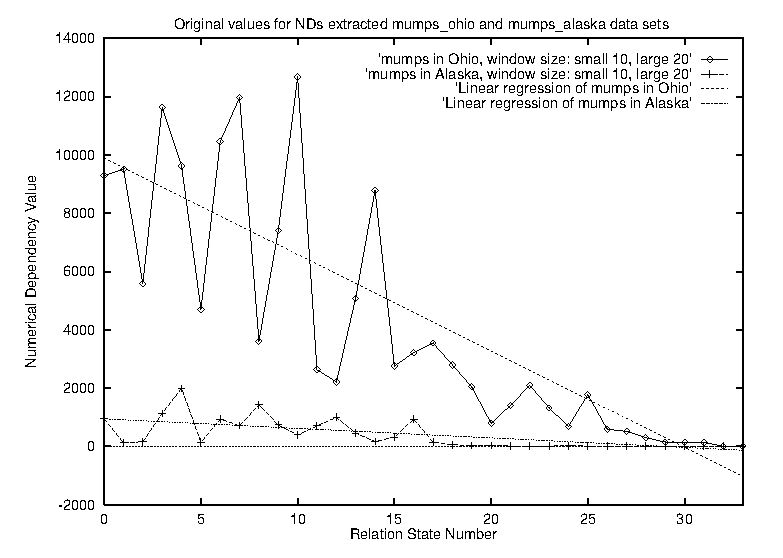
\includegraphics{figures/mumps_postv.eps}}}
\caption{\label{graph:mumps_ohio_1}{Original data values of mumps
cases in Ohio and Alaska from 1957 - 1989}}
\end{figure}

The results obtained for a small sequence size of 5 years and a large
size of 10 years were $\Delta_{mp} \models$ \resp{10}{5} ($ohio\downarrow_r \wedge^0 alaska\downarrow_r$)
together with persistence results of the following abbreviated form
\pers{10}{5} ($ohio\downarrow_r \wedge^0
alaska\downarrow_r$). Clearly, these results tell us 
that the number of cases in mumps is falling, continuously, without
significant fluctuation.  
Applying a simple pattern matching algorithm for comparing exact
trend within a sequence we find that \safe{12}
($ohio$ $\downarrow$ $\leadsto$ $ohio$ $\uparrow$ $\leadsto$ $ohio$ $\downarrow$) holds for Ohio. Therefore
although we have found the general trends to be downward there are
peaks within larger sequences.
For a comparison between the
number of cases in Alaska and Ohio we increased the sequence sizes to
12 and 20 and found, continuously throughout the sequence that the
following persistence rule holds: \pers{20}{12}
($ohio\downarrow_r \wedge^2 alaska\downarrow_r$). We see that the lag in
the downward trends (ohio lags alaska by 2 years) may provide an
indication that the number of 
cases falling is correlated with geographical regions. Obviously
expert knowledge is required to confirm this; \cite{fay98b} discusses
issues of correlation versus causality noting that it is generally not
clear in which situations correlation can lead to causality. It may be
foolish to infer a causal relationship solely on the basis of the
discovery of a lagged correlation. This is the subject of much study
with further references provided in \cite{gmp97}.

\smallskip
A complete description of the series is provided by ($ohio\downarrow_r
\wedge^1 alaska\downarrow_r$) $\leadsto$ ($ohio\downarrow_r
\wedge^2 alaska\downarrow_r$). We find the same rule from applying
discordance instead of linear regression. This rule concisely presents
the behaviour of the sequence. It is obtained from three 12 year sequences
with some overlap (there is 33 years of data) and compressed, for
clarity, so that $\sigma \leadsto \sigma$
becomes $\sigma$. We  
omit presentation of such description rules for longer time series.
We can see from these simple results how properties of NDs over time
can be succinctly characterised within our logic. We now move on to a
slightly more interesting example.

\medskip



\begin{figure}
\centerline{\scalebox{0.7}{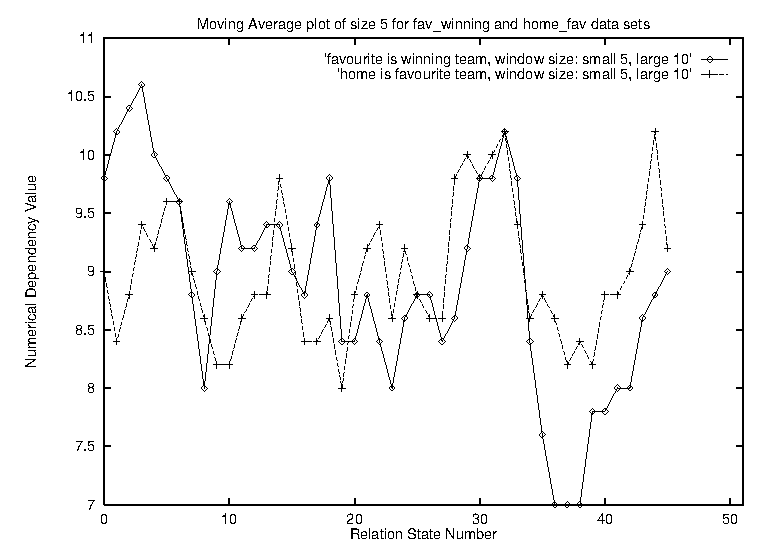
\includegraphics{figures/fav_winning_postv.eps}}}
\caption{\label{graph:profb_1}{Moving Average data set values of two NDs
from NFL season data 1989-1991}}
\end{figure}



In Figure~\ref{graph:profb_1} we present the changing ND values for
two NDs obtained from relations containing Football Data. Each week of
the season, for three seasons from 1989 to 1991, details of team
results were stored in a database together with details of the
favourite team for each match. We obtained two NDs from the relation
$YEAR$  $WEEK$ $\to^k$ $FAV\_TEAM\_WIN$ and $YEAR$  $WEEK$ $\to^k$
$HOME\_FAV$. These NDs correspond to the number of favoured teams
winning and the number of home favourites, respectively, within a
particular week.
We note that each relation contained $YEAR$  $WEEK$
 $DAY$ representing the day the match was played
on. Figure~\ref{graph:profb_1} shows
the two lines relating to changes in each ND. We can see no clear
trend in this figure for moving averaged data.

\medskip

For the two NDs we found the following property from the moving
average record of points with each moving average of size 5,
$\Delta_{NFL} \models$ \pers{10}{5} ($HOME\_FAV$ $\uparrow_r \wedge^0$
$FAV\_TEAM\_WIN$ $\uparrow_r$) suggesting that an
increase in the home team winning is correlated with an increase in
the favourite team winning. This persistence property expresses the fact
concisely and we can perhaps infer from this that the home teams are
most often the favourite team. Additionally, we examined the original
and differenced data set for patterns in sequences of 5 weeks and
found none. It is 
clear that the nature of the data contains no underlying trend 
expressing only the strong correlation between NDs.

\medskip

Before presenting the results obtained from time series data we
formally define the moving blocks bootstrap.

\subsection{The Moving Blocks Bootstrap}\label{subsec:tr_mbb}
\index{Moving Blocks Bootstrap}
\index{Bootstrap Resampling}


We introduce the Moving Blocks Bootstrap for verification of short
range event rules and provide details of its efficacy discussing the
results we found from its application in later sections.

\begin{definition}[Moving Blocks Bootstrap for Relation Sequences]\label{def:mbb}
\begin{rm}
Given a relation sequence $\{ r_1, r_2, \ldots, r_N \}$
we construct blocks of relations where $MB_t$ is a block containing
$b$ relations such that $MB_t = \{ r_t, r_{t+1}, \ldots, r_{t+b-1} \}$
and there are $N - b+ 1$ blocks where $t = 1, 2, \ldots, N-b+1$. We
then resample $k$ moving blocks uniformly with replacement from $\{
MB_1, MB_2, \ldots, MB_{N-b+1} \}$ where $N \sim bk$. This may be repeated any number of times.$\quad\Box$
\end{rm}
\end{definition}

\smallskip

\begin{figure}[ht]
\centerline{\scalebox{0.7}{\includegraphics{../Event_theory/mbb.eps}}}
\caption{\label{fig:mbb} All possible blocks of size 4 for a relation sequence}
\end{figure}

The moving blocks bootstrap forms an empirical distribution and this
distribution is the proposed bootstrap approximation. For a block
length $b$ all possible contiguous blocks of length $b$ within the
time series are available for selection. In \cite{et93} each moving
blocks bootstrap sample has an AR(1) model fitted to it to estimate
the parameter $\beta$. Results decreased upon an increase in the block
size, perhaps allowing us to infer that dependency was based on the
previous few points only (to any significant degree). The potential to
sample all possible contiguous blocks of a given size $b$ allows all
possible relationships of length less than or equal to $b$ to be sampled.


\subsection{The Moving Blocks Bootstrap for Large Data Sets}\label{subsec:tr_vlmbb}
\index{Moving Blocks Bootstrap}
\index{Bootstrap Resampling}


We now propose a new Moving Blocks Bootstrap for creating resamples
when either the temporal relation sequence or the time series contain
too many points for a resample to obtain meaningful results. For
example this may be a stock over 10 years. We may form a series of
values, which are fixed in ordering, so that this 10 year sequence may
be compressed into resamples of, say, 2 years each. This will then create a
manageable sequence size for property discovery across multiple
resampled sequences.

\begin{definition}[Moving Blocks Bootstrap for Large Relation Sequences]\label{def:vlmbb}
\begin{rm}
Given a relation sequence $\{ r_1, r_2, \ldots, r_N \}$ we construct a
resampled relation sequence of size $n$, where $N \gg n$, with the
order of the resampled relation sequence preserved from the original
data set.
We construct blocks of relations where $MB_t$ is a block containing
$b$ relations such that $MB_t = \{ r_t, r_{t+1}, \ldots, r_{t+b-1} \}$
and there are $N - b+ 1$ blocks where $t = 1, 2, \ldots, N-b+1$. 
We then divide the sequence into $R$ regions where $R = \frac{N}{n}$.
From each region $R_i$, $0 \le i \le R-1$ we resample 1 moving block
uniformly from $\{ MB_{(i*n)+1}, MB_{(i*n)+2}, \ldots,
MB_{(i*n)+n-b+1} \}$ and append 
the block to our resampled sequence. Order is therefore preserved for
$n$, a given 
size. This may be repeated any number of times. $\quad\Box$
\end{rm}
\end{definition}

\smallskip

\begin{figure}[ht]
\centerline{\scalebox{0.7}{\includegraphics{../Event_theory/vlmbb.eps}}}
\caption{\label{fig:vlmbb}A large relation sequence and a resample}
\end{figure}

Given that the random block selection for the moving blocks bootstrap
for large relations is order preserving we must be careful in our
random block selection to ensure that we do not initially select a
block at the end of the sequence to which no blocks can be
appended. To remedy this we propose that the sequence is divided into
a number of regions $n$, from Definition~\ref{def:vlmbb}. From these
regions we select one block randomly. For example, a 10 year sequence
may be divided into 24 regions, of 5 months each, from which a block
of one month is selected from each. This would then allow reasonable
knowledge discovery on a manageable sequence with relationships
between either NDs or time series preserved within blocks and the
 ordering of the sequence is preserved in the
resamples. Alternatively, we could use standard moving blocks
resampling with smaller sample sizes and sorting each resample into
the correct temporal order; this would create more randomness in the
resamples. 

\section{Time Series Data Results}\label{sec:tr_tsares}
\index{Time Series Data Results|(}


We now examine more complex temporal data sets. We 
assume that the data is restricted to numerical data alone, although
if the data were stored in a suitable manner then NDs
could easily apply. When analysing time series we are not seeking to
discover what a complex statistical analysis could not; indeed much of
our logic is based on statistical functions. Instead we are looking
for a concise representation that might convey specific properties
which hold at a certain time or throughout time and we express these
with our logic. The logic details properties in a machine
understandable form. 


\medskip

For the following study we focused on financial stocks from the FTSE
100. We analysed stocks in similar sectors seeing if there are general
properties from which we can infer information, concentrating on
financial, oil and retail sectors. We highlight some of the results
found and remark that all applications discovered possibly useful
properties. In the following we initially present results based on each category
of data, discussing the results with respect to the sequence size
selected; we follow this with a discussion of how these properties
might relate to the data they represent in the real world. A summary
of results is presented for each data set in
Tables~\ref{tab:tr_arg_deb_res}, ~\ref{tab:tr_bp_sh_res},
and~\ref{tab:tr_al_hfx_res}. As a precursor to this discussion we
remark that the absence of a property with respect to sequence sizes
chosen by the user, when evaluated with results for other sequence
sizes, may itself tell us much about the data set.

\section{Case Study I}\label{sec:tr_case1}

We present results for Debenhams ($db$) and the Arcadia Group ($ag$),
summarised in Table~\ref{tab:tr_arg_deb_res}, in an extended form
which highlight characterisation of the discovery of
property. Subsequent studies are abbreviated to avoid repetition and
we refer to this sequence as $\Delta_{ad}$. Due to the similarity
between regression and discordance results, we concentrate on results
obtained using linear regression. We note that we are now dealing
exclusively with time series and not ND values; this is primarily due
to the availability of time series data and, as we have seen, the
limited availability of data satisfying ND sets. We note that all
results are equivalent to those that may be found for ND sets in a
temporal relation sequence and could feasibly be expressed with NDs,
though this may often be impractical. 


{\line
\begin{table}[ht]
\begin{center}
\begin{tabular}{|c||c|} \hline 
\multicolumn{2}{|c|}{\bf Debenhams and Arcadia Group } \\ \hline
 Description of data set & 199 days of closing prices   \\ \hline
\multicolumn{2}{|c|}{In all formulae: Arcadia Group ($ag$) and
Debenhams ($db$)} \\ \hline
\multicolumn{2}{|c|}{\bf Trend Discovery} \\ \hline
Original Data Set       &  $\Delta_{ad}$ $\models$ \resp{80}{1} ( $ ag \downarrow$) \\
 			 & $\Delta_{ad}$ $\models$ \resp{80}{1} ($ db \uparrow$) \\\hline
\multicolumn{2}{|c|}{\bf Property Discovery} \\ \hline
Original Data Set	&   $\Delta_{ad}$ $\models$ $\bm^{160}$
 ( $ag \downarrow_r$ $ \wedge^{0}$ $db \downarrow_r$ ) $\leadsto$  ( $ag
 \downarrow_r$ $ \wedge^{0}$$ db \downarrow_r$)\\
			&  $\Delta_{ad}$ $\models$  \pers{10}{5}  ($ag
 \uparrow_r \wedge^{0} db \uparrow_r$ ) \\
			&   $\Delta_{ad}$ $\models$ \pers{20}{10}  ($ag \uparrow_r
 \wedge^{0} db \uparrow_r$ )\\
			&  $\Delta_{ad}$ $\models$ \pers{20}{10}  ($ag \downarrow_r \wedge^{0} db\downarrow_r$ )  \\
			&   $\Delta_{ad}$ $\models$ \pers{30}{15}
 ($ag \downarrow_r \wedge^{0} db \downarrow_r$ ) \\
			&  $\Delta_{ad}$ $\models$ \pers{40}{20}  ($ag
 \downarrow_r \wedge^{0} db \downarrow_r$)\\
			&  $\Delta_{ad}$ $\models$\pers{80}{40}  ($ag
 \downarrow_r \wedge^{0} db \downarrow_r$)\\
			&  $\Delta_{ad}$ $\models$ \resp{160}{80}  ($ag \downarrow_r
 \wedge^{0}\downarrow_r$)\\
			&  $\Delta_{ad}$ $\models$ \resp{160}{80}
 ($ag \uparrow_r \wedge^{1} db \downarrow_r$ )   \\ \hline
Moving Average          &  \\
Window size:3	&  $\Delta_{ad}$ $\models^3$ \pers{20}{10}  ($ag
 \downarrow_r \wedge^{0} db \downarrow_r$),
 found 12 times \\
Window size:8	&  $\Delta_{ad}$ $\models^8$  \pers{80}{40}  ($ag \downarrow_r
 \wedge^{0} db \downarrow_r$)     \\\hline
Moving Block Bootstrap          &  \\ 
Block Size: 5	&  $\Delta_{ad}$ $\models^3$ \pers{20}{10}  ($ag
 \downarrow_r \wedge^{0} db \downarrow_r$ )     \\
Block Size: 10	&  $\Delta_{ad}$ $\models^{3}$  \resp{40}{20}  ($ag
 \downarrow_r \wedge^{0} db \downarrow_r$)     \\
	&  $\Delta_{ad}$ $\models^{3}$   \resp{80}{20}  ($ag \downarrow_r
 \wedge^{0}\downarrow_r$) \\
All for MA Block Size:3		&  $\Delta_{ad}$ $\models^{3}$ \resp{80}{20}
 ($ag \uparrow_r \wedge^{0} db \uparrow_r$)    \\ \hline
Differenced Series        & \\
		  & $\Delta_{ad}$ $\models$  \resp{80}{20}  ($ag
 \downarrow_r \wedge^{0} db \downarrow_r$) \\ 
		&   $\Delta_{ad}$ $\models$  \resp{80}{20}  ($ag
 \uparrow_r \wedge^{0} db \uparrow_r$)  \\ \hline
2nd Order Differenced Series      & \\
		    &  $\Delta_{ad}$ $\models$  \resp{80}{20}  ($ag
 \uparrow_r \wedge^{0} db \downarrow_r$)\\ 
		&   $\Delta_{ad}$ $\models$ \resp{80}{20}  ($ag
 \downarrow_r \wedge^{0} db \uparrow_r$)    \\ \hline
\end{tabular}
\end{center}
\caption{\label{tab:tr_arg_deb_res} Results for 199 days of Arcadia and
Debenhams Group }
\end{table}
}

\subsection{Original Data Analysis}\label{subsec:tr_analysis}

Properties extracted from the original data set are based solely on
the original data values upon which our property discovery algorithms
are applied. We first discuss looking for trends as properties. We see
in Table~\ref{tab:tr_arg_deb_res} that we obtained safety trends, for
a sequence 
size 80, \resp{80}{1} ($ag \downarrow$) for the Arcadia Group and \resp{80}{1}
($db$ $\uparrow$) for Debenhams. This states that in every 80 day sequence
there is at least one day when the stock goes up or down! This may seem
obvious but these two results together suggest that Debenhams might be
performing better than Arcadia. The procedure to obtain these naive trend
rules uses a simple pattern matching algorithm. We also found 
persistence rules of the form 
 \pers{20}{10}  ($ag \uparrow_r \wedge^{0} db \uparrow_r$ ) and  \pers{20}{10}
($ag \downarrow_r \wedge^{0} db \downarrow_r$ ). The former
persistence rule was 
discovered at five points in the complete sequence and the latter was found to
hold at the very beginning of the series. This corresponds with the
actual values which are generally within a downward trend apart from
an initial upward trend depicted by their moving averages in Figure~\ref{graph:deb_199_2}. Increasing the sequence size shows that
persistence rules for upward trends do not hold at all for larger
sequence sizes and so we conclude that upward trends within the series
are short and that the general trend is down, exemplified by
\pers{80}{40} ($ag \downarrow_r \wedge^0 db \downarrow_r$). Similarly,
the safety 
trend descriptions indicate that Debenhams might be performing better
that Arcadia.
			

\subsection{Moving Average Analysis}\label{subsec:tr_mav_analysis}
\index{Moving Averages}
\index{Jackknife Resampling}

The goal of creating a moving average of a time series is to smooth
the series so that outliers, potentially caused by noise or outside
effects, have a weakened influence on the data discovery
process. They are widely used in stock data analysis \cite{rm97}.
 We conducted experiments with a jackknife procedure for moving
average smoothing, 
whereby the moving averages for each sequence are calculated
successively with one data point removed and then averaged. We obtained a
slight increase in smoothing over the standard moving average but not
enough to justify the additional computational cost in its use and so
this was not employed. 

\smallskip

Moving average results in general back up the results provided by the
original data set. We note that smoothing tends to obscure short
term trends so that persistence or guarantee rules which hold in the
original data set may not hold for a moving average
series. Additionally, the size of the window for moving 
averages increases the {\em spreading} effect of a single data
point. To illustrate we found far fewer properties for larger moving
average windows. Figure~\ref{graph:ma3_12} shows how a larger window
size increases the spread for the moving averages, reducing the
amplitude of both peaks and troughs.


\begin{figure}
\centerline{\scalebox{0.7}{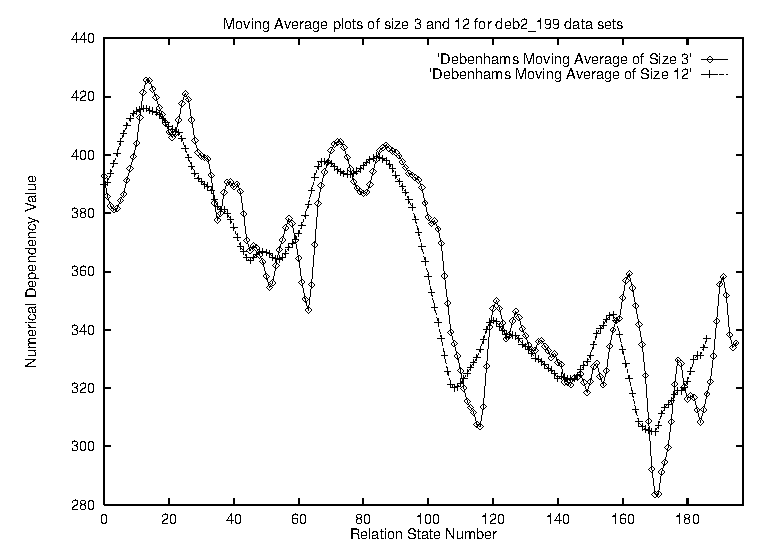
\includegraphics{figures/arg2_199_w20_b40_postv.eps}}}
\caption{\label{graph:ma3_12}{Moving Average Data
values for two window sizes, 3 and 12}}
\end{figure}


\subsection{Differenced List Analysis}\label{subsec:tr__diff_analysis}
\index{Differenced List}

In Time Series Analysis differencing is used by statisticians to
remove trend from a series, as we outlined in Section~\ref{sec:tl_tsa}.
Similarly we may obtain the differenced values for a data set upon
which we run our property detection algorithms. This may lead to the
discovery of properties which then represent seasonal and not trend
behaviour. We refer to Table~\ref{tab:tr_arg_deb_res} which
present some results for differenced lists. Due to the complex nature
of stock behaviour we can not be sure if the properties for
differenced lists detail seasonal or just noisy behaviour. The result
of a first differencing provides very similar results to the original
and moving average properties. Namely, that the behaviour of the two
stocks is closely related with response and persistence properties
detecting either joint upward or downward trends. Extending this to a
second order differencing we find that this shared behaviour is no
longer discovered. What can we infer from this?  For a conclusive
answer we would have to ask a fund manager, however, we note
that perhaps their seasonal behaviour is not related or that the
stocks are affected by different events outside of their
relationship. In such a way we can use our algorithms for the
discovery of seasonal properties.


\subsection{Moving Blocks Bootstrap Analysis}\label{subsec:tr_mbb_analysis}
\index{Moving Blocks Bootstrap}

The moving blocks bootstrap, defined in Section~\ref{subsec:tr_mbb},
is used within time series analysis for model creation based on the
assumption that temporal relationships do not occur for a time longer
than the size of the blocks used to create the moving blocks
resamples. The moving blocks resamples may then be recreated many
times to obtain a model based on these resamples. We created moving
blocks resamples of our time series. Interesting properties were found
and though we believe some properties for some resamples to be
spurious we could have removed these via repeated application of the
moving blocks bootstrap and intersection of the results.
Applying the moving blocks bootstrap also allows for properties to be
discovered which may be violated in sequences without such a
rearrangement, perhaps caused by noise.

\medskip

The order of the moving blocks resamples is random. It is therefore
highly likely that spurious trends may be found for the moving blocks.
\resp{80}{20} ($ag \downarrow \wedge^{0} db \downarrow$ ) and
\linebreak \resp{80}{20}
($ag \uparrow \wedge^{0} db \uparrow$ ) were both found with a block size
of 10 days. This implies, we believe, two things. Firstly, that the
behaviour of the two stocks is closely related both sharing either
upward or downward trends. Secondly, the difference between small and
large sequence sizes is quite significant implying that it is likely
that blocks will occur to create an upward trend shown in the second
response rule. The data miner needs to choose sequence sizes carefully
in such cases. For a block size 5 we found \pers{20}{10} ($ ag \downarrow$
$\wedge^0$ $ db \downarrow$ ), which backs up both the original and moving
average results. The variation of block size allows us to make
conclusions about the nature of the trends. For 5 and 10 days we found
properties with upward or downward trends suggesting that these stocks
possess trend behaviour longer, in general, than these block
sizes. This is, however, a feature of the financial market in general.


\section{Case Study II}\label{sec:tr_case2}

We present results for two oil stocks BP (bp) and Shell Oil (sh),
summarised in Table~\ref{tab:tr_bp_sh_res}, in an abbreviated form.

{\line
\begin{table}[ht]
\begin{center}
\begin{tabular}{|c||c|} \hline 
\multicolumn{2}{|c|}{\bf BP and Shell } \\ \hline
 Description of data set & 242 days of closing prices   \\ \hline
\multicolumn{2}{|c|}{In all formulae: British Petroleum ($bp$) and Shell ($sh$)} \\ \hline
\multicolumn{2}{|c|}{\bf Trend Discovery} \\ \hline
\multicolumn{2}{|l|}{\bf Techniques} \\ \hline
BP   & $\Delta_{oil}$ $\models^w$ $\bm^{15}$ \diam$^1$ ($bp
\downarrow$) \\
	& $\Delta_{oil}$ $\models$ $\bm^{50}$ \diam$^4$
($bp \downarrow$  $\leadsto$  $bp \uparrow$ $\leadsto$ $bp \downarrow$
$\leadsto$ $bp \uparrow$ ) \\
Shell & $\Delta_{oil}$ $\models$ $\bm^{15}$ \diam$^1$ ($sh\uparrow$) \\
	& $\Delta_{oil}$ $\models$ $\bm^{50}$ \diam$^3$ ($sh\uparrow$
$\leadsto$ $sh\downarrow$ $\leadsto$ $sh\uparrow$ )  \\\hline
\multicolumn{2}{|c|}{\bf Property Discovery} \\ \hline
Original Data Set  & $\Delta_{oil}$ $\models$ \pers{30}{15}  ($bp \downarrow_r
		\wedge^{0}sh\downarrow_r$), found 7 times \\
		&  $\Delta_{oil}$ $\models$ \resp{45}{15}  ($bp\downarrow_r \wedge^{0}sh\downarrow_r$)\\
		&  $\Delta_{oil}$ $\models$ \pers{60}{30}  ($bp\downarrow_r \wedge^{0}sh\downarrow_r$)\\ 
		&  $\Delta_{oil}$ $\models$ \resp{90}{45}  ($bp\uparrow_r \wedge^{0}sh\uparrow_r$) \\
		&  $\Delta_{oil}$ $\models$ \resp{180}{90}
		($bp\uparrow_r \wedge^{0}sh\downarrow_r$) \\ 
		& $\Delta_{oil}$ $\models$ \resp{180}{90}  ($bp\uparrow_r \wedge^{0} sh\uparrow_r$) \\ \hline
Moving Average  & $\Delta_{oil}$ $\models^3$ $\bm^{180}$
 ( $bp\downarrow$ $ \wedge^{0}$ $sh\downarrow$ ) $\leadsto$  ( $bp\downarrow_r$ $ \wedge^{0}$$sh\downarrow_r$) \\
Block Size: 3 	&  $\Delta_{oil}$ $\models^3$ \pers{60}{30}  ($bp\uparrow_r \wedge^{0}sh\uparrow_r$)\\
		&  $\Delta_{oil}$ $\models^3$ \pers{60}{30}  ($bp\downarrow_r \wedge^{0}sh\downarrow_r$) \\
Block Size: 8 	&  $\Delta_{oil}$ $\models^8$ \pers{30}{15}  ($bp\downarrow_r \wedge^{0}sh\downarrow_r$),
		found 7 times\\
Block Size: 10	&  $\Delta_{oil}$ $\models^{10}$ \pers{60}{30}  ($bp\uparrow_r \wedge^{1}sh\uparrow_r$) \\\hline
Moving Block Bootstrap          &  \\
Block Size: 15		&  $\Delta_{oil}$ $\models^{8}$ \resp{60}{30}  ($bp\downarrow_r \wedge^{0}sh\downarrow_r$) \\ 
Block Size: 25		&  $\Delta_{oil}$ $\models^{8}$ \resp{100}{50}
		($bp\downarrow_r \wedge^{0}sh\downarrow_r$) \\
All for MA Block Size: 8 & \\ \hline
Differenced	&  $\Delta_{oil}$ $\models$ \resp{60}{30}  ($bp\downarrow_r \wedge^{0}sh\downarrow_r$)
		\\  \hline
2nd Order Differenced	&  $\Delta_{oil}$ $\models$ \resp{60}{30}  ($bp\downarrow_r
		\wedge^{0}sh\uparrow_r$) \\ 
		&  $\Delta_{oil}$ $\models$ \resp{60}{30}  ($bp\uparrow_r
		\wedge^{0}sh\downarrow_r$) \\ 
 			& $\Delta_{oil}$ $\models$  \resp{60}{30}  ($bp\downarrow_r
		\wedge^{0}sh\downarrow_r$) \\  \hline
\end{tabular}
\end{center}
\caption{\label{tab:tr_bp_sh_res}Results for 242 days of BP and Shell
		from Dec 1997 to Oct 1998} 
\end{table}
}

The original values again emphasise a strong relationship between the
two data sets at smaller sequence sizes. We experimented with large
sequence sizes and found 
\linebreak \resp{180}{90} ($bp \uparrow_r \wedge^0 sh \downarrow_r$).
Two points
about this are worth noting. Firstly, the disparity in trend in not
immediately clear from a graph, cf. Figure~\ref{graph:bp_11mn_1},
which exhibits much similarity. The initial upward trend of BP stocks
may be viewed as {\em masked} by a number of short term downward
trends which the properties suggest.
Secondly, the data set consists of
only 242 points (days). Yet we are looking for sequences of 180 days
which implies that there is no sequence which does not overlap with
another. This response rule is therefore perhaps not quite so strong
though still interesting. 

\medskip

Finally, we briefly refer to Table~\ref{tab:tr_al_hfx_res}. This
consists of stock prices for two newly converted building societies in
their first 100 days on the market. Though we found properties they do
not present themselves as showing much similarity. We can infer that
the behaviour of the market at the time of launch is itself more
important that what the company is. Tests showed that different stocks
over different time periods tend towards not discovering properties as
opposed to discovering properties which represent disparate
behaviour.  Additionally, of the properties discovered we see a number
of spurious lags which do not suggest strong related behaviour. This
is a validation of our discovery process. 
 
{\line
\begin{table}[ht]
\begin{center}
\begin{tabular}{|c||c|} \hline 
\multicolumn{2}{|c|}{\bf Halifax and A \& L Banks } \\ \hline
 Description of data set & 100 days of closing prices   \\ \hline
\multicolumn{2}{|c|}{In all formulae: Alliance \& Leicester ($al$) and
Halifax ($hfx$)} \\ \hline 
\multicolumn{2}{|c|}{\bf Trend Discovery} \\ \hline
 A \& L   & $\Delta_{ha}$ $\models$ $\bm^{10}$ \diam$^1$ ($al$ $\uparrow$) \\
 Halifax  & $\Delta_{ha}$ $\models$ $\bm^{10}$ \diam$^1$ ($hfx$ $\downarrow$)\\
	&  $\Delta_{ha}$ $\bm^{20}$ \diam$^1$ ($hfx$ $\uparrow$) \\
		&        \\\hline
\multicolumn{2}{|c|}{\bf Property Discovery} \\ \hline
Original Data Set  & $\Delta_{ha}$ $\models$  \resp{60}{30}  ($al\downarrow_r \wedge^{6}hfx\downarrow_r$)\\
		& $\Delta_{ha}$ $\models$  \resp{60}{30}  ($al\uparrow_r \wedge^{-3}hfx\downarrow_r$)\\
		\hline
Moving Average  & $\Delta_{ha}$ $\models^5$  \pers{20}{10}  ($al\uparrow_r \wedge^{0}hfx\uparrow_r$)\\
Block size: 5	& $\Delta_{ha}$ $\models^5$  \resp{60}{30}  ($al\uparrow_r \wedge^{-3}hfx\downarrow_r$) \\
		& $\Delta_{ha}$ $\models^5$  $ \bm^{60}$ ( $al\downarrow_r$ $ \wedge^{6}$
		$hfx \downarrow_r$)\\ \hline
Moving Block Bootstrap          &  \\ 
Block size: 5	& $\Delta_{ha}$ $\models^5$  \pers{20}{10}
		($al\downarrow_r \wedge^{0}hfx\uparrow_r$)\\ 
MA Block size:5 & \\ \hline
\end{tabular}
\end{center}
\caption{\label{tab:tr_al_hfx_res} Results for first 100 days trading
		of Halifax and Alliance \& Leicester Banks }
\end{table}
}

\subsection{Real-World Analysis}\label{sec:tr_real_analysis}


\begin{figure}
\centerline{\scalebox{0.7}{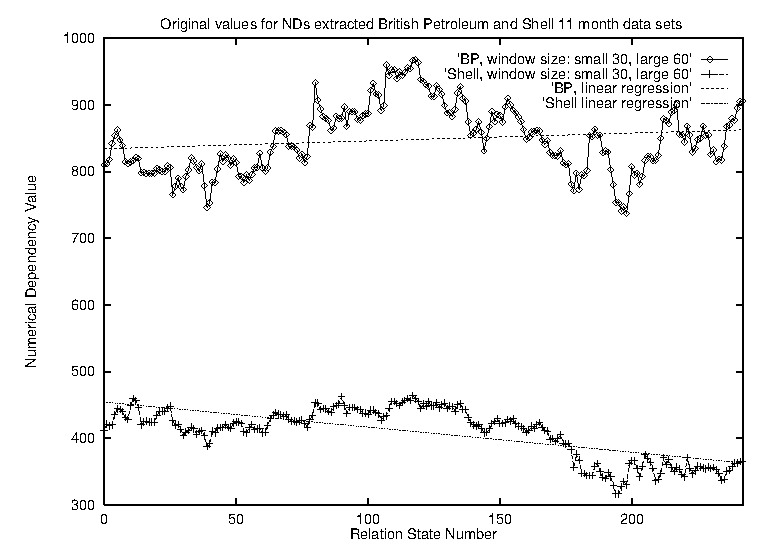
\includegraphics{figures/bp_11mn_sh_11mn_postv.eps}}}
\caption{\label{graph:bp_11mn_1}{Time series of BP and
Shell from 1 Dec. 1997 to 1 Nov. 1998}}
\end{figure}

Our first analysis
focuses on BP and Shell. Under a story entitled ``bad times for the
oil industry'' in the Lex column of the Financial Times, November 4
1998, it was discussed how the oil industry has suffered in recent
months though some recent results (third quarter) posted by BP show
that a 35\% drop in profits is good news in comparison with a more
than 50\% drop by Shell prices. We can see from
Figure~\ref{graph:bp_11mn_1} that BP ($bp$) has been outperforming
Shell ($sh$) in
terms of recent performance. We discovered however that the stocks are
related in short term performance, as we would expect. We found that
in Jan and Feb the following persistence property held \linebreak \pers{90}{60}
($bp$ $\uparrow_r \wedge^0$ $sh$ $\uparrow_r$), a period of gradual
rise in both stocks. We also found that \linebreak \pers{60}{30} ($bp$
$\downarrow_r \wedge^0$ $sh$ $\downarrow_r$) holds from day 160 in
Figure~\ref{graph:bp_11mn_1}, relating to the downward trend that
begins in May. With a smaller
sequence similar results 
were obtained though we also discovered that \pers{10}{5} ($bp$ $\downarrow_r
\wedge^0$ $sh$ $\uparrow_r$) held in September 1998; this opposite behaviour
may be due to external influences.

\medskip

In Figure~\ref{graph:deb_199_2} we show the moving averaged sequence
for two companies, Debenhams ($db$) and the Arcadia Group ($ag$) since
January 28 1998. On January 28 1998 Debenhams demerged from its former
owner the
Arcadia Group. We can see from Figure~\ref{graph:deb_199_2} that
recently Debenhams has performed better 
than Arcadia due to, based on expert opinion, the fact that Debenhams
sells many different goods whereas Arcadia concentrates more on fashion and
is expected to perform poorly in the light of a recession. In August
1998, corresponding with a downturn in the economy, we found
\pers{30}{15}  ($db$ $\downarrow_r \wedge^0$ $ag$ $\downarrow_r$) and
for the recent good performance of Debenhams we found \pers{10}{5} ($db$
$\uparrow_r \wedge^0$ $ag$ $\downarrow_r$), amongst other rules. The
regression coefficient used to determine trend may be significantly
small. However the trend still exists and we can subscript trends by
their regression value or even extend this to a {\em fuzzy} value to denote the
significance of the trend.   


\begin{figure}
\centerline{\scalebox{0.7}{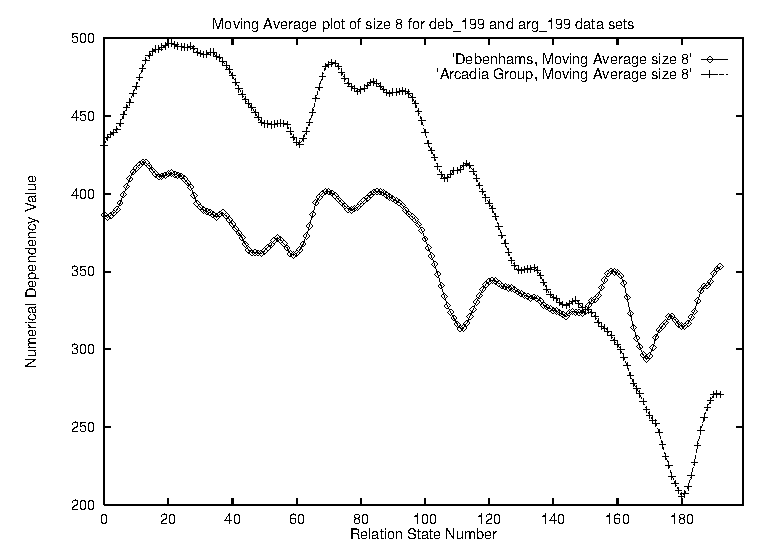
\includegraphics{figures/deb_199_w15_b30_postv.eps}}}
\caption{\label{graph:deb_199_2}{Moving Average values for
Debenhams and Arcadia Group since demerger on Jan 28 1998}}
\end{figure}


It is imperative that the two sequence sizes are well chosen by the
user. It would help if the user had expert knowledge of any kind of
seasonality duration. If $n > \frac{m}{2}$ where $n$ is the
smaller sequence size and $m$ the larger then there will be an overlap
of at least one point in all $n$ size subsequences of $m$. This is to
be avoided and is advisable as a lower bound on the sequence size
relationship. 

\smallskip

 For BP and Shell we found no properties for sequence
sizes of less than 15 days on a moving blocks resampled sequence. This
may imply that trends relate to longer term behaviour.
We
found within all results that we tested the moving blocks results
confirmed previously found persistence results and occasionally
presented spurious response properties. Repeated application to
numerous moving block sequences and intersecting the results removed
these spurious properties. Similarly differencing provided similar
results in the data we tested; this may be due to forcing sequences
and studying local linearity removes the need for longer term trend
removal.
\index{Time Series Data Results|)}


\section{Moving Blocks Bootstrap for Large Relations}\label{sec:mbb_large}



\begin{figure}
\begin{minipage}{7cm}
\centerline{\scalebox{0.5}{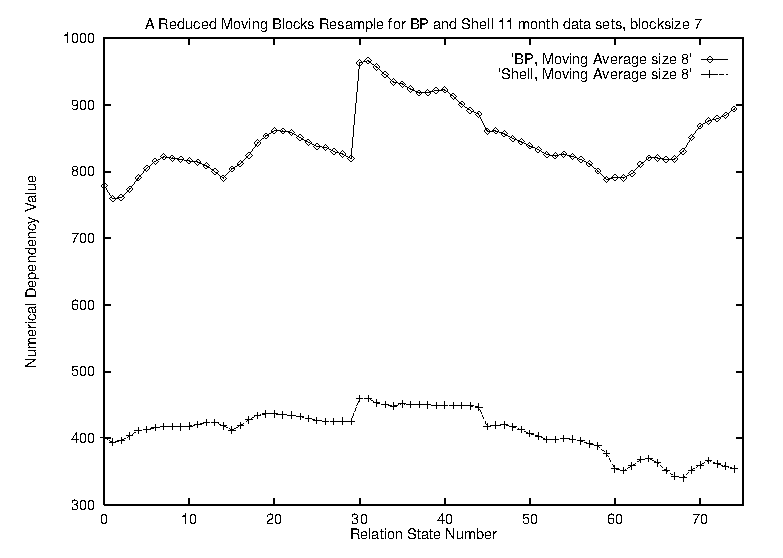
\includegraphics{figures/bp_11mn_w30_b60data_postv.eps}}}
\caption{\label{graph:bp_11mnfixblock1}{Reduced moving blocks
samples for BP and Shell moving average data, 78 points from 11
regions and blocksize of 7 points}}
\end{minipage}
\hfill
\begin{minipage}{7cm}
\centerline{\scalebox{0.5}{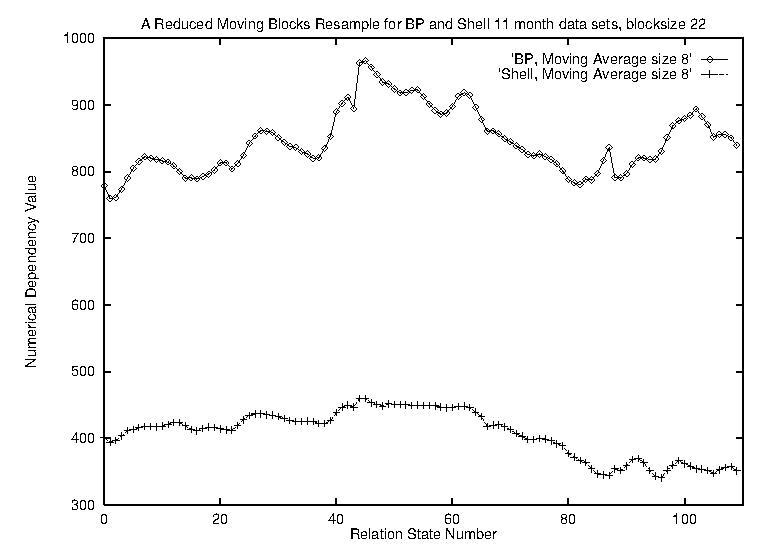
\includegraphics{figures/bp_11mn_w45_b90data_postv.eps}}}
\caption{\label{graph:bp_11mnfixblock2}{Reduced moving blocks
samples for BP and Shell moving average data, 110 points from 5
regions and blocksize of 22 points}}
\end{minipage}
\end{figure}


The use of the moving blocks bootstrap for large relations allows
smaller resampled relation sequences to be created from the original data set. 
We can see in Figure~\ref{graph:bp_11mnfixblock1}, for example,
a moving block resample of only 78 points from the original data set
of 242 points, which closely resembles the original data set. The need
for repeated iterations of the moving blocks samples is shown in the
results found. We found $\Delta_{oil} \models$ (\pers{30}{15}
($bp \uparrow_r \wedge^0  sh \uparrow_r$)), and, in abbreviated form, \resp{30}{15} ($bp \uparrow \wedge^0
sh \uparrow$), \resp{30}{15} ($bp \downarrow \wedge^0
sh \downarrow$), and \resp{30}{15} ($bp \uparrow \wedge^0
sh \downarrow$) in one resample, which was not found in the original data
set. We also found \resp{90}{45} ($bp \uparrow \wedge^0
sh \uparrow$) and \resp{90}{45} ($bp \downarrow \wedge^0
sh \downarrow$), the latter of which was not found for the original
data set.

\medskip

We draw the following conclusions from using the moving blocks
bootstrap for very large relations:
\begin{itemize}
\item A visual analysis shows that Figures~\ref{graph:bp_11mnfixblock1} and
~\ref{graph:bp_11mnfixblock2} in comparison with
Figure~\ref{graph:bp_11mn_1} of the original data set show the
similarities for the two smaller resampled sequences. Such similarity can be 
exploited for knowledge discovery when a series contains a significant
number of points to obtain a valuable {\em synopsis} of the sequence.
\item That the resampled original, and possibly even the resampled
moving average, data sets of reduced size, contains too many fluctuations, and as such allows the
generation of properties which may be {\em generally} false of the
data. For example, two resampled blocks may be concatenated and they
may violate, or satisfy, a trend which holds, or does not.
\item The use of the moving blocks bootstrap to cut down the number of
points needed to examine for the discovery of properties, is, like the
property discovery process itself, highly dependent on the choice of
both {\em block size} and the {\em region size} from which the blocks
are selected. If the block size is too small with respect to the
region size it will not reflect trends sufficiently well. It it is too
large then it will closely resemble the original sequence, which we
might as well use in this situation. There is of course the additional
problem of selecting a suitable blocksize in relation to the sequence
sizes for property discovery. A blocksize smaller than a sequence size
is more likely to result in fewer properties discovered, particularly
when the resampled series is much smaller than the original.
\item Even for a small number of points the reduced moving blocks
bootstrap is able to detect relationships, and properties, across
series reasonably well.
\end{itemize}

Resampling to create reduced size sequences is valuable when the data
set is too large to mine in full for property satisfaction.

\section{Critical Analysis}\label{sec:tr_crit_an}

Our methodology for the discovery of properties has a number of
problems. Particular properties are more likely to be discovered for
particular sequence size choices. A response rule \resp{m}{n} is much
more likely to hold when $m \gg n$ wherein the guarantee property
\diam$^n$ is given more time in which to occur. Clearly, the data
miner has the choice of setting these parameters.

\medskip

Another questionable area is that whether all properties discovered
are interesting. This is certainly not true. For example, we must be
very careful with guarantee properties to ensure that they are not
presented as knowledge discovery without good reason. This begs the
question, what makes a property interesting? As properties become more
complex they are more likely to represent an interesting feature of
the dataset. We must be careful with properties that are not {\em
boxed}, i.e., not safety properties. For example, an {\em ordered
persistence property} of the form $\sigma_1 \leadsto$ \pers{m}{n} $\sigma_2$
can be found for any persistence property apart from the very start of
the time sequence, given that $\sigma_1$ can be an arbitrary formula
which is true in some sequence before \pers{m}{n} $\sigma_2$ holds.
Therefore it is of little value in knowledge
discovery terms. However, if this property occurs similarly at regular
points(within $\bm^{p}$) then we have discovered something potentially
very interesting about the data.

\medskip

The use of time series statistics has been shown to be both efficient and
useful. We have found our representation of lags in the logic to be
equivalent, though developed independently by what we considered to be a requirement, to the representation in time series of {\em lag
operators} \cite{end95}, where the value is ignored and only the lag
itself is important. We conducted some tests to examine the efficacy
of the lag. This was particularly important as most properties
discovered found 0 lag. We overlapped our time series by a number of
points $n$ and then removed the extraneous $n$ points at the beginning
and end of the respective series. We found similar properties to hold
but with the lag to be the same value as the overlap. For example, we
found \pers{30}{15} ($ag \downarrow \wedge^{0} db \downarrow$ ) became
\pers{30}{15} ($ag \downarrow \wedge^{3} db \downarrow$ ) when the overlap
was 3 points for the retail data set. As we extended
this the number of properties discovered decreased due to the lower
likelihood of behaviour reoccurring at regular intervals. Additionally,
for small sequences, overlaps also resulted in fewer properties. Upon
the advice of \cite{ko90} we restricted lags to $\frac{n}{4}$ given
that otherwise stronger lags are found at the highest lag length where
there are far fewer points to correlate.  \cite{end95} suggests
beginning with the longest plausible lag length over which there may
be a possible relationship. 


\begin{figure}
\centerline{\scalebox{0.7}{\includegraphics{figures/timeplot_200_postv.eps}}}
\caption{\label{graph:prop_disc_time}{Time for discovery of
response and persistence properties for varying small and large
sequence sizes and small varying only (for a large sequence size)
within a 398 point data set}}
\end{figure}

In Figure~\ref{graph:prop_disc_time} we provide details of the times
required for discovery of response, \resp{m}{n}, and persistence, \pers{m}{n},
properties for different sequence 
sizes. We found that sequence size increasing for both $m$ and $n$ at
a fixed rate (with $m = 2n$) was
similar to increasing only the sequence size $n$ with respect to
property discovery for large sequence size $m = 200$. This is due to
most of the computation 
time working on the discovery of safety and guarantee properties with
respect to $n$. Also there are small fluctuations in the time
required. We found this was due to some sequences satisfying fewer
initial safety and guarantee properties leading to faster checking
time for response and persistence
properties. Figure~\ref{graph:prop_disc_time} shows that properties
can be discovered very efficiently.

\medskip
In Section~\ref{subsec:temp_mine} we discussed a number of alternative
approaches to temporal data mining. We now compare our approach to
that of \cite{bt98} which uses a restricted temporal logic in conjunction with
probabilities and an interestingness measure for rule discovery from
input strings. In the example we 
now discuss \cite{bt98} obtain the probability of an event $e$ from
dividing its frequency in a string by the total length of the string
such that each {single} event has an interestingness of exactly 1.
Within the domain of a {\ttb sendmail\tte} program, having 31
commands, rules were discovered, such as ({\em sigblock} ${\cal N}$
{\em setpgrp}) ${\cal N}$ {\em vtrace} 
with an attached interestingness value of 43.16, where
{\em sigblock}, {\em setpgrp}, and {\em vtrace} are commands within the
program. Additionally ({\em sigblock} ${\cal B}_k$ {\em stepgrp}) ${\cal B}_k$
{\em vtrace} is also discovered with the same interestingness value
suggesting that $\cal N$ would be redundant if the subscript $k$ were
given explicitly. Our logic may, if applied to a similar domain,
represent the latter rule as ({\em sigblock} $\leadsto$ {\em setpgrp})
$\leadsto$ {\em vtrace}, assuming 
that we allow program commands as atoms. We can also
use properties to denote how often these rules occur within a
given period of time. For example, a response rule within every two
minute period is expressed by \resp{120}{n} ({\em sigblock} $\leadsto$
{\em setpgrp}) $\leadsto$ 
{\em vtrace}, where $n$ is the time to execute these commands. An extension
to our work could be the creation of our own {\em interestingness}
measure based on a property being more interesting if the ratio of the
smaller to larger sequence size is closer to 1. This could also be
applied from the larger sequence size to complete sequence size.
\cite{bt98}
also restrict the size of maximum string length for discovery such
that the rules found cover only a small size of the original input
string. Rules within sequences allow for discovery over longer time
periods as we have seen; this is aided by our use of regression.

\section{Similarity Assessment}\label{sec:tr_sim_ass}
\index{Time Series Similarity}

Much recent work looking at assessing the similarity of two time
series \cite{alss95,frm94,dgm97,rm97}, as discussed in
Chapter~\ref{chap:review}, concentrates on transformations applied to
Fourier sequence representation of a time series.  As a novel
contribution to this field we add our use of property discovery for
similarity assessment. From suitable sequence sizes we
discover properties which may represent related behaviour across
sequences telling us about trends, lags, and seasonal events.

\medskip

\cite{rm97} apply Euclidean distance
to moving average time series to see if two time series are similar. 
\cite{dgm97} applies transformation functions so that the scaling of
the two time series being compared need not necessarily be the same
over the same number of points. This is a useful feature which would
also be of value for property discovery. Time series are considered
similar if there exists an approximate transformation function which maps one
series to the other. \cite{dgm97} considers linear functions only. We
now propose another definition of similarity based on sequence sizes
such that two sequences are similar if all properties discovered for a
particular sequence size depict equivalent behaviour. For example,
both moving average trends or seasonal behaviour after differencing
would always be equivalent for both time series within all properties
found. The work of \cite{alss95} does not allow outliers and requires
sequences to be of the same length whereas
property discovery from moving averages would have the effect of
already weakening any outliers. Our form of knowledge discovery will
also have the advantage in that properties may be discovered which
correspond to a particular range of the sequence within which they may
exhibit similar behaviour before diverging.
Most studies of similarity
would not provide a decent result in this instance, particular if we
are looking for a linear transformation function.  Though we do not
explicitly allows translation across time points of our time series
this, as we have shown, is represented by the presentation of lags or
lead values within series. 

\medskip

Finally, we remark that if a querying system were implemented for our
logic the similarity would be able to be enumerated via a set of
queries which may or may not hold.

\section{Discussion}\label{sec:tr_disc}



If a database query language were to incorporate the ability to search
for properties within a temporal database then any DB user would be
able to ask questions concerning possible properties that he suspects
might hold in the data. We have shown that this can be achieved using
our logic in polynomial time. The current range of statistical
functions available in DBMS need only minimal extension to include time
series functions and then it would be entirely feasible to express
relationships in a readily understandable form such as that of our
logic.
 
\medskip
 
We have presented our logic for NDs in temporal sequences. Results
applied to temporal relation sequences and time series have shown our
logic capable of providing succinct characterisation of the data to a
{\em system user}. The response and persistence properties that we
discovered are both useful and 
valid and may be applicable in a decision support
environment. Properties discovered within a DBMS might be
desired to hold for all future points in which case they could be
elevated to the status of integrity constraints. 
Extensions to this work include the implementation of a
querying system and additional algorithms for property discovery.

\medskip
We presented a generic algorithm for the discovery of knowledge using
the temporal classification of properties and then refined this to a
specialised algorithm for response and persistence rule discovery. The
algorithm is generic in that it applies to all discovery which uses
the classification hierarchy, of which our model in
Figure~\ref{fig:model2} is one particular instance.
The similarities between
these and the generic algorithms given in \cite{man96,man97} point to
similarities within the data mining model. Work on a unified theory of
data mining will require a set of generic mining algorithms which can
be specialised for many different approaches \cite{jmw96}.
\medskip 

The goals of \cite{bt98} were to generate unexpected predicates,
expressed in a restricted temporal logic, from sequential databases or
strings. This has application in rule discovery from categorical data
whilst our logic relies on numerical data alone, though in the case of
NDs this may be based on categorical data. The restriction of a
maximum string length is similar to our requirement of a given
sequence size. A sequence of size $n$ satisfying $\sigma_1 \leadsto
\sigma_2$ differs only from $\sigma_1 {\cal B}_k 
\sigma_2$ found in a string of size $n$ in that we allow overlap,
assuming that $\sigma_1,\sigma_2$ occur in sequences. The need
for restriction is 
that the interestingness measure is always higher for longer sequences
implying that a rule representing the complete input string is always
the most interesting whereas our motivation is to enable property
discovery, possibly relating to, say, seasonal behaviour.
Both properties and measures, such as interestingness, are of value
within data mining.

\smallskip

Much recent knowledge discovery research has been concerned with
finding out if two time series are in some sense similar
\cite{frm94,alss95,dgm97}. Our logic has the expressive power to represent
similarities as properties or standard sentences of the logic from
which we can easily deduce similarities between two time series. As an
avenue for further work it
would be interesting to expand this using, perhaps, intersections of
properties found for similarity assessment.

\chapter{Summary and Conclusion}\label{chap:conclusion}

In this thesis we have presented a novel methodology for data
mining in indefinite and temporal databases. We have demonstrated
throughout this thesis how NDs are useful within the data mining
process. In the thesis we have provided empirical
evidence that our dynamic use of resampling is effective for
determination of a sample size; this may have applications for other
NP-complete problems. Also, we have shown that our temporal logic for
time sequences (of NDs) is easily applicable and a viable addition to
the data mining toolkit. 



\section{Contribution of this work}\label{sec:conc_contrib}

We have outlined a general framework for data mining in non-standard
databases, not previously considered. In the most informal sense, we
take sets of approximations to FDs, in this thesis we consider only
NDs, and use statistical functions and tools to infer conclusions on
patterns within the data; in the domain of indefinite information we
use resampling in a dynamic fashion based upon mean, variance
or standard errors satisfied by sets of NDs. In the temporal
domain we can use resampling or moving averages to form new sequences
from the original values of ND set satisfaction, which change over
time, to determine specific properties which may hold within the
temporal relation sequences. Our use, in a general sense, of
statistical functions upon large sets or sequences of NDs to discover
information can be viewed as a {\em second order data
mining}. We evidence this general approach in two domains though we
speculate that there may be many more applications in other domains,
ranging from spatial to active databases.

\medskip

We now describe in more detail the specific contributions made by this work.
Chapter~\ref{chap:numdep} has shown that NDs are viable dependencies
within the relational model, extending the intentions of Grant and Minker
\cite{gm85b,gm85a} when they introduced NDs as extensions of FDs for
greater flexibility in schema specification. Principally we use the
chase for NDs, proven to be sound and complete herein, for the
inference of NDs; we show this to be decidable. In this way the chase allows for ND inference
to be tested in database applications, although this may be
intractable. We also show how NDs themselves 
may be used within data mining or database design algorithms to
approximate FD sets, demonstrated via an evolutionary database design
algorithm. NDs were shown to effectively extend the class of methods
approximating FD sets in a relation.  
ND mining may be limited in the sense that for an ND $X \to^k A$, if A
is a category of exactly $k$ elements, then the ND only
tells us that all elements occur in A; it may be considered more
informative if this were not the case, perhaps in continuous
domains. Also, the mean ND combats 
this problem by providing more information within a data mining context.
A metric for ND sets is
also provided which we employed within our work on indefinite
information in relations.

\medskip

We studied indefinite information in relations, concentrating solely
on the consistency problem, known to be NP-complete. We created a
general randomised procedure which made use of a chase developed using
NDs for indefinite relations and a dynamic resampling technique. We
chose to employ resampling to be able to make statistically valid
inferences from a sample of possible worlds taken from an indefinite
relation. Each possible world satisfies an ND set. Resampling from a
sample of possible worlds allows us to determine approximate values of
variance and standard deviation. Our randomised algorithms require a
sufficient sample size upon which to apply their selection functions
so as to obtain decent approximations to FD set satisfaction. We found
that as the variance and standard deviation change with the degree of
indefinite cells in a relation it is possible to apply resampling
iteratively on increasing sample sizes until an approximate fixpoint
is reached. Independent of our work, \cite{jl96} argue, in a position
paper, for dynamic sampling to be adopted within data mining instead of
naive sampling techniques in use. Our work does just this. Extensive
simulations on these methods showed that the chase is of use in
a larger relations with correspondingly larger domain sizes and that
the resampling is useful for providing an 
upper bound on the number of possible worlds required.

\medskip

In Chapters~\ref{chap:templog} and~\ref{chap:tempresult} we
demonstrate the practicality of NDs in temporal databases. Given that
changing ND sets, from a user supplied template, may only vary on
their branching factor we can view the sequence of changes as a time
series. Considering specific time series analysis techniques as a
basis we developed a logic using modal operators to discover rules
which a sequence may satisfy. Necessary restriction of the formulae of
our temporal logic to properties, used within program verification,
proved to be highly useful for knowledge discovery. We make no grand
claims on the formalisation of our logic with respect to it being a
panacea for time series data mining though we note that it allows for
knowledge to be represented succinctly and has an easily
understandable semantics; an important yet understated factor of many
knowledge discovery systems. Further theoretical analysis of the
logic, outside the 
scope of this thesis, is definitely required. It is most likely that
logics for time series analysis could be developed in many different
ways.

\medskip

Properties of temporal logic which were defined for program
verification have been extended for data mining purposes. The
specifications required in programs for correctness analysis lends
itself well to knowledge discovery where changing inputs over time may
frequently satisfy similar conditions. Properties of temporal logic
have not, in the limits of our experience, been considered for data
mining. 

\medskip

As we have shown this thesis is a contribution to the arena of data
mining in both techniques and tools. We show that NDs are valuable within
data mining and believe that the techniques of our randomised algorithms,
dynamic resampling, and temporal logic have clear application.  We feel
that our hypothesis of NDs for data mining in non-standard relations
has been vindicated via the work demonstrated herein.

\section{Applications}

There are a number of applications within which this work can be
used, which we now detail:
\begin{itemize}
\item Our general framework can be transferred to other domains. For
example, in a spatial database we can, after input of a FD set as a
template, mine for ND set satisfaction of this template and
then employ (or develop) statistics which are pertinent to spatial
data sets; \cite{kah96} presents $k$-predicates for spatial data
representation of the form, for example, $close\_to(x,lake) \wedge
close\_to(x,road)$ implying that $x$ is {\em close to} both a lake and a
road which could also be summarised as an ND object $\to^k$ site in a
relation CLOSE\_TO(object,site).  We believe that we could discover
and use patterns represented
by such NDs in spatial databases.
\item We can employ dynamic resampling to generate a {\em
representative} sample size in a number of NP-complete problems. 
\item Our logic can be applied to any time series for property
detection. 
\item We can mine any database for ND set satisfaction. The metric
presented in Chapter~\ref{chap:numdep} can be applied to any set of
NDs, assuming a finite domain.
\end{itemize}

\section{Directions for future research}

There are many directions for possible future research posed by this
work, in domains of dependency theory (for data mining), temporal/time
series data mining, and indefinite data mining. We begin by
considering a direct extrapolation of this research.
 
\subsection{Open Problems}

This thesis has the following {\em important} open problems:
\begin{itemize}
\item The implementation of efficient mining procedures for NDs in
standard relations. Extensions for NDs to the dynamic dependencies presented
in \cite{Via87,Via88} as outlined in Section~\ref{subsec:temdat}
warrant further analysis, with regard to both database theory and data
mining research
\item A study of algorithms to create weak Armstrong Relations, as
defined in Section~\ref{subsec:nd_ar}, for
Database design purposes. 
\item A theoretical analysis of our dynamic resampling
algorithm, WORLD\_LIMIT, is required.
\item We conjecture that
implication for ND sets with the chase is an NP-complete problem. It would be
interesting to search for special classes of NDs or relations,
possibly incomplete, within
which the chase procedure is polynomial in execution time. This work
would be similar in spirit to that of \cite{ll97c}.
\item Implementation of a query system based on our temporal logic,
NDLTL.
\item An in-depth study of expressiveness of non-standard logics, such
as NDLTL, is required. This would be particularly useful with a view to
data mining applications.
\end{itemize}

We elaborate on some of these issues in the next section.

\subsection{Further work}

In the arena of NDs we could further extend their applicability by the
creation of scaling and translation functions, as used for
transformation functions in time series similarity
\cite{alss95}. These functions have direct application when we are
dealing with relations that are of vastly different sizes. As noted in
Section~\ref{sec:nd_disc} we could also investigate more sophisticated
algorithms for the mining of NDs in standard relations. This work
could make use of many heuristics including hypergraph
transversals. One example using ND semantics may be that we do not 
have to consider mining the remainder of a relation if we have found a
partition for an ND whose branching factor is greater than over half
the number of tuples in the relation. Dynamic Dependencies introduced
for FDs by \cite{Via87} would have a highly useful semantics if
extended to NDs, as motivated by the example in
Section~\ref{subsec:temdat}. It would be of value to mine corporate,
and other, databases for the presence of these relationships whereby
the branching factor of an ND may determine subsequent branching
factors of itself and other NDs later in the timeline.
	
\medskip
The work on searching for a satisfying possible world within an
indefinite relation provides numerous avenues for further
study. Clearly, it would be highly interesting to use real-world
scheduling representations to see how useful our ND approximation sets
are. We could also 
analyse rates of convergence for our resampling process with respect to the
nature of an indefinite relation and the FD set
used. Further study of this within
such dynamic algorithms as our procedure would be very useful, both in
terms of data mining and of relevance to a multi-disciplinary research
field. Additionally, phase transitions in indefinite
relations, referred to in Section~\ref{sec:cp_disc}, would be a most
interesting further study, complementing previous 
phase transition work with dependencies and relations that have a real
information content. 

\medskip

Finally, our work on temporal data mining requires a thorough study of
the logic we have created. The inclusion of time series functionality
makes the expressive nature of the logic unclear. The flexibility of
the logic means that it is easily extended. Further
research into time series behaviour may provoke the need for
additional operators. We believe that this would include functions
designed specifically for the analysis of non-linear relationships.
We would also like to
be able to spend time developing sophisticated algorithms which use
this logic for temporal data mining. One such example would be to
discover a suitable sequence size upon which to conduct the data
mining process. Error functions from regression analysis could also be
incorporated into the logic.  Such would be desirable from a 
systems point of view.  

\section{The Evolution of Data Mining}

Data Mining is a rapidly expanding field, not least due to a
concentrated global effort into the extraction of information from
data. The state of the art applications are still led by recent
theoretical developments. There will be a significant increase in the
use of statistical developments within data mining products. Our use
of resampling in both the temporal and indefinite domains shows how
such novel processes can be applied easily and effectively. More data
mining tools will incorporate sampling and resampling in the quest for
information which may {\em characterise} a data set.

\medskip

There have been recent criticisms that data mining, as yet, is not
fully integrated with the database interface \cite{man97,joh97,cha98}. It is
only a matter of time before the next relational database upgrade
includes a data mining toolkit. For clarity and ease of use, there is
potential for the inclusion of such items as NDs and temporal logic. This,
and other, logics would make use of statistical functions within the 
database query language.  

\medskip
The process of data mining will mesh with databases so that predictors
and forecasting can be assessed at any time, which may be NDs or other
dependencies. These predictors themselves may be mined and
the technique of building our logic
upon dependencies as atoms is perhaps a first step in this direction. 

\section{Conclusions}

The field of knowledge discovery is rapidly expanding due to the
ever-increasing amounts of data being stored. The user-centric
processes of data mining are extending the fields of statistics,
artificial intelligence and machine learning into a new science
\cite{fu96}. Our work has made significant use of database,
statistical, and logical theory to develop a new general framework for
data mining in temporal and indefinite relations.






{\setlength{\baselineskip}{14pt}
\bibliography{bibliography/Assoc,bibliography/Rough_sets,bibliography/Tabu,bibliography/Comp_books,bibliography/NPcomplete,bibliography/Concept_latt,bibliography/DB_design,bibliography/Databases,bibliography/Databases4,bibliography/Dependency,bibliography/Fuzzy,bibliography/Logic_Ddb,bibliography/Logic_Prog,bibliography/Logic_Theory,bibliography/Know_disc,bibliography/Know_disc2,bibliography/Philosophy,bibliography/Maths,bibliography/Prob_DBs,bibliography/Dynamics,bibliography/Mining,bibliography/Armstrong,bibliography/ga_pap,bibliography/Sim_An,bibliography/Warehouse,bibliography/time_s,bibliography/ilp,bibliography/Time_dbs,bibliography/Prob,bibliography/Spatial_dm,bibliography/Patterns,bibliography/Game_Theory,bibliography/Learning,bibliography/Neural,bibliography/Lattices,bibliography/Random,bibliography/Entropy,bibliography/Stats,bibliography/modelling,bibliography/Optimize,bibliography/Logic_time,bibliography/db_evolution,bibliography/Bootstrap_Apps,bibliography/Object_db,bibliography/Automata,bibliography/Concurrency,bibliography/ethan,bibliography/Incomp_inf,bibliography/Ecommerce,bibliography/Int_constraints,bibliography/Regression,bibliography/Temp_mine,bibliography/Education,bibliography/Sequence}
}

\appendix
\chapter{The Consistency Problem: Supplemental Results}\label{app:con_prob}

We now provide additional results for the consistency problem. In
Table~\ref{tbl:fd_set_used} we detail the FD sets referred to in the
following figures. All of the mean values referred to for the average
number of worlds required were obtained within batchs, each of 500
runs. The results in this appendix reinforce those presented in
Chapter~\ref{chap:consistency}.  All relations used, with respect to the
FD sets in Table~\ref{tbl:fd_set_used}, contain exactly those
attributes within the respective FD set as the schema and no more. 


{
\line
\begin{table}[ht]
\footnotesize{
\begin{center}
\begin{tabular}{|c||c||c||c||c||c||c||c|}
\hline
{\bf Set 1} & {\bf Set 2} 	& {\bf Set 4} 	& {\bf Set 6} & {\bf Set 7}	& { \bf Set 11} & {\bf Set 15}	& {\bf Set 17} \\ \hline \hline
$A \to B$ &	$A \to BC$	&  $C \to AB$	&  $D \to ABC$ & $AB \to D$ 	& $A \to B$ 	&$A \to BCD$	& $A \to B$ \\
$D \to C$ &	$D \to C$     &  $B \to AC$	&  $AB \to D$ & $D\to ABC$ 	& $D \to C$ &		& $B \to C$ \\
	&			&  		&  $A \to B$ & & $BC \to A$ &		& $C \to D$  \\
	&			&  		&  $B \to A$ & &  		&	&  \\\hline
\end{tabular}
\end{center}
}
\caption{\label{tbl:fd_set_used} FD sets used in
Figures~\ref{graph:4.3w} to~\ref{graph:histo2}}
\end{table}
}

For an FD set X $\to$ Y, where $\mid$ Y $\mid > 1$, we split this into
a set of FDs such that for all A $\in$ Y we have X $\to$ A for
expression as NDs in simulations.  This is justified given that from X
$\to^k Y$ we can infer, for all A $\in Y$, X $\to^k$ A.

\section{Average Number of Worlds Required}


We present examples showing the average number of worlds
required in batches by our chase and hill-climbing algorithm in
figures~\ref{graph:4.3w} to~\ref{graph:4.16w}.  We can see immediately
that the average number of worlds required is very small. We
hypothesise that within our random relations it is relatively easy to
generate a definite world using algorithms~\ref{alg:gen}
and~\ref{alg:chase-gen}. The average number of worlds is reduced for
larger relations with respect to a fixed domain size. Investigation
has shown this to be due to ND sets being satisfied closer to the
domain size, whilst the presence of additional tuples, with respect to
a fixed domain size, increases the number of redundant values within
indefinite cells which the chase procedure can remove. This is
particularly true of relations with larger arity indefinite cells, see
figures~\ref{graph:4.2w}, and~\ref{graph:4.13w}. Figures~\ref
{graph:4.4w} and~\ref{graph:4.12w} show this is less likely when
relations have smaller arity indefinite cells. 

\begin{figure}
\begin{minipage}{7cm}
\centerline{\scalebox{0.5}{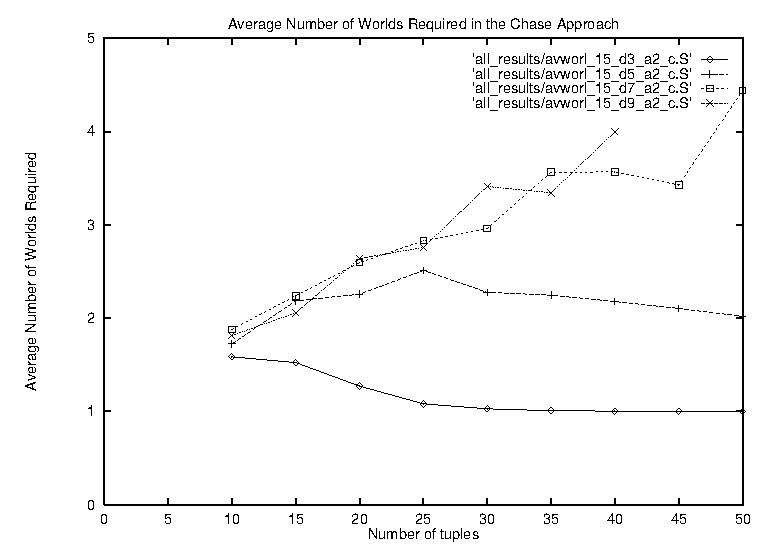
\includegraphics{figures/w15_d3_a2_c.eps}}}
\caption{\label{graph:4.3w} {Average Number of Worlds Required by
the chase and hill-climbing approach for FD set 15, domain sizes 3 -
9, maximum indefinite cell arity 2 }}
\end{minipage}
\hfill
\begin{minipage}{7cm}
\centerline{\scalebox{0.5}{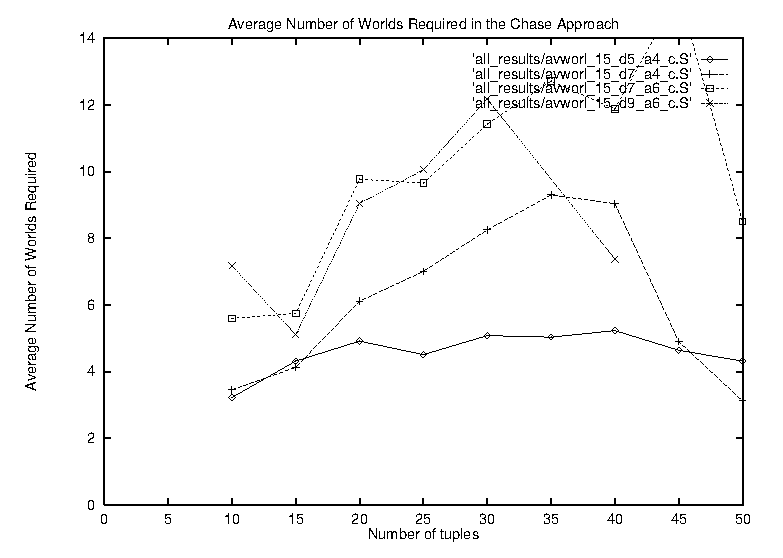
\includegraphics{figures/w15_d3_a4_c.eps}}}
\caption{\label{graph:4.2w} {Average Number of Worlds
Required for FD set 15, domain sizes 5 - 9, max indefinite arity 4 - 6}}
\end{minipage}
\end{figure}

We also note that the small number of average worlds is in sharp
contrast to the number of worlds required by the naive {\em generate and
test} algorithms to obtain similar results. We are vague as to an
exact relationship due to the varying nature of both the indefinite
relations and FD sets.

\begin{figure}
\begin{minipage}{7cm}
\centerline{\scalebox{0.5}{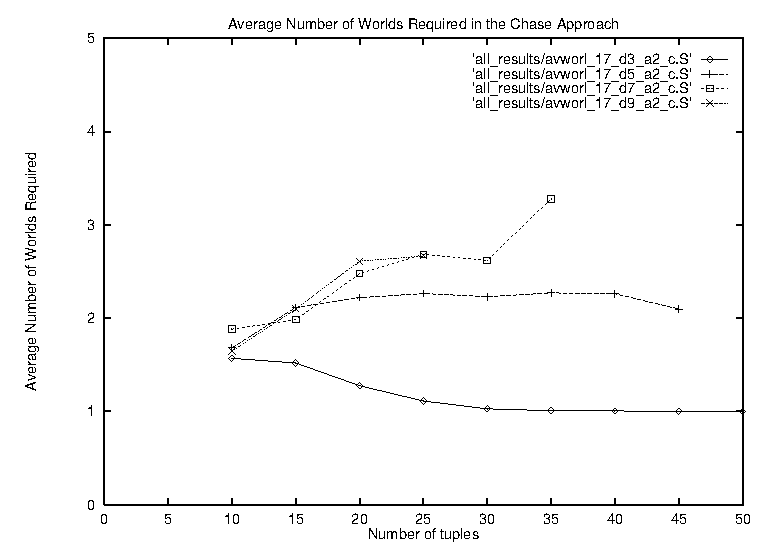
\includegraphics{figures/w17_d3_a2_c.eps}}}
\caption{\label{graph:4.4w} {Average Number of Worlds
Required for FD set 17, domain sizes 3 - 9, max indefinite arity 2}}
\end{minipage}
\hfill
\begin{minipage}{7cm}
\centerline{\scalebox{0.5}{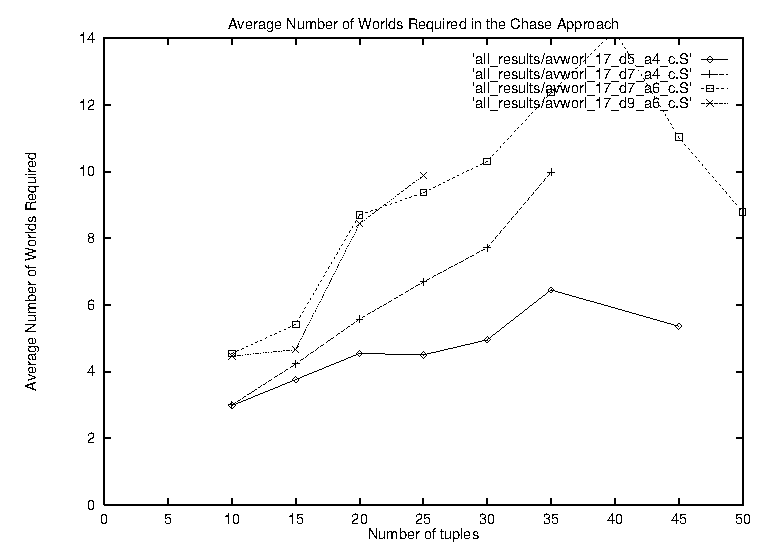
\includegraphics{figures/w17_d3_a4_c.eps}}}
\caption{\label{graph:4.5w} {Average Number of Worlds Required for FD
set 17, domain sizes 5 - 9, indefinite cell arity 4 - 6}}
\end{minipage}
\end{figure}




\begin{figure}
\begin{minipage}{7cm}
\centerline{\scalebox{0.5}{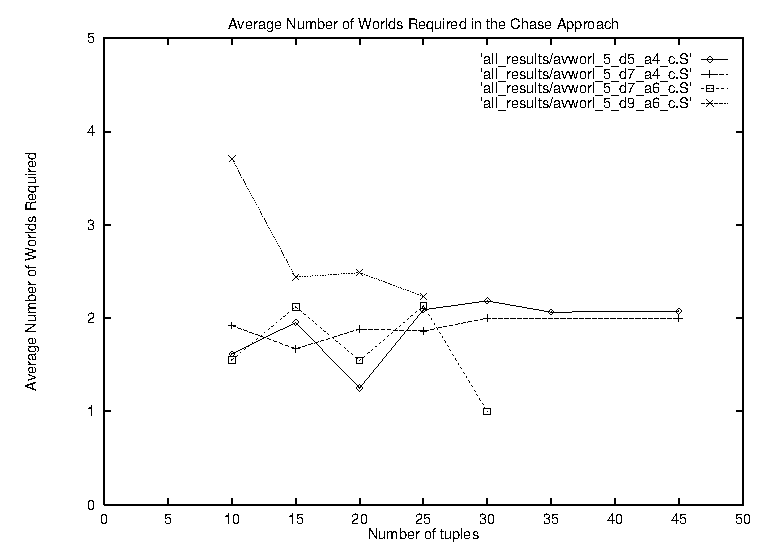
\includegraphics{figures/w5_d3_a4_c.eps}}}
\caption{\label{graph:4.10w} {Average Number of Worlds
Required for FD set 5, domain size 5 - 9, indefinite cell arity 4 - 6}}
\end{minipage}
\hfill
\begin{minipage}{7cm}
\centerline{\scalebox{0.5}{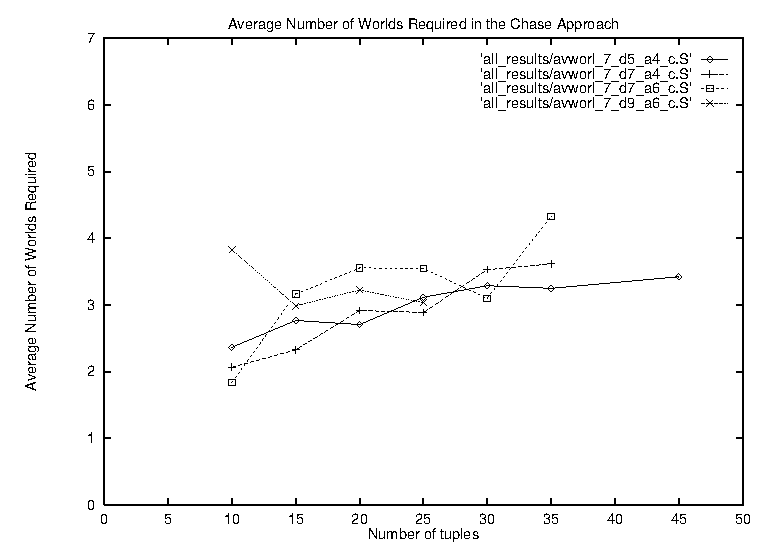
\includegraphics{figures/w7_d3_a4_c.eps}}}
\caption{\label{graph:4.16w} {Average Number of Worlds
Required for FD set 7, domain size 5 - 9, indefinite cell arity 4 - 6}}
\end{minipage}
\end{figure}


\begin{figure}
\begin{minipage}{7cm}
\centerline{\scalebox{0.5}{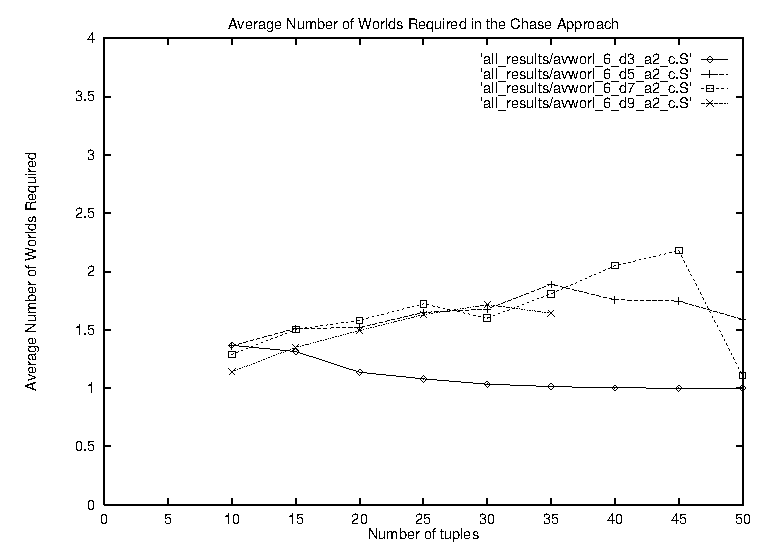
\includegraphics{figures/w6_d3_a2_c.eps}}}
\caption{\label{graph:4.12w} {Average Number of Worlds
Required for FD set 6, domain size 3 - 9, indefinite arity 2}}
\end{minipage}
\hfill
\begin{minipage}{7cm}
\centerline{\scalebox{0.5}{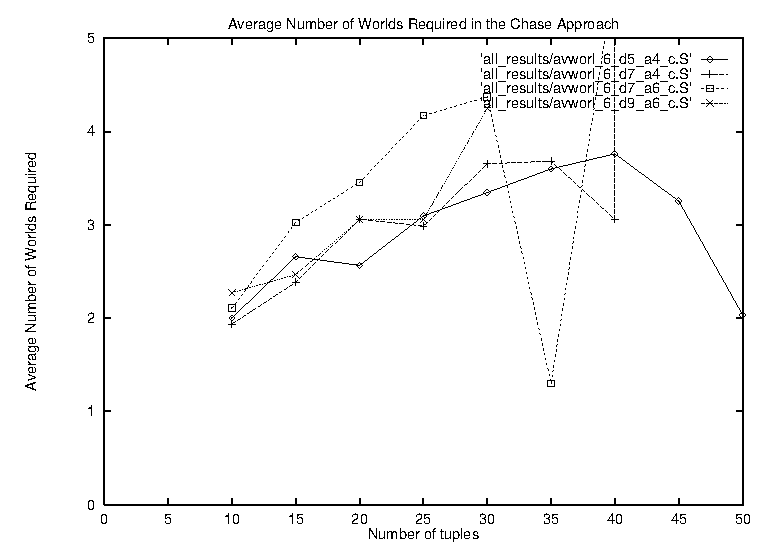
\includegraphics{figures/w6_d3_a4_c.eps}}}
\caption{\label{graph:4.13w} {Average Number of Worlds required 
for FD set 6, domain size 5 - 9, indefinite arity 4 - 6}}
\end{minipage}
\end{figure}





\section{Average Proximity to FD sets}

We now discuss the proximity of our results to that of an FD set. The
increasing proximity to an FD set as relation size increases is due to
the domain size remaining fixed. Normalisation of our measure for ND
sets, a prospect for future work, would remedy this.

\medskip

We draw the following conclusions concerning proximity:
\begin{itemize}
\item On average the naive and chase procedures produce very similar
results. We emphasise that our relations were created in a uniformly
random manner. As such in the real world it may be highly likely that
a relation with indefinite information may perform better with respect
to utilising the chase and hill-climbing approach. This speculation is
enforced by the encouraging discovery that the chase procedure produce
slightly better results when a relation is sparse in indefinite cells
in arity in either attributes on the left or right hand side of
dependencies, as detailed in figures~\ref{graph:5.6}
to~\ref{graph:5.5}. 
\item Proximity to functional satisfaction increases, on average, with
an increase in the number of attributes being determined. We can see
these differences in figures~\ref{graph:6.1} and~\ref{graph:5.15}. The
difference in this case is slight but this was enforced by all
results. This is due to additional attributes being examined within
the hill-climbing process. The random nature of the relations
generated did not provide us with any pathological data
which might contradict this.
\item Whether the relation is in BCNF or non-BCNF did not, in the
data assessed, affect the results. We did not expect this to be otherwise.
\end{itemize}


\begin{figure}
\begin{minipage}{7cm}
\centerline{\scalebox{0.5}{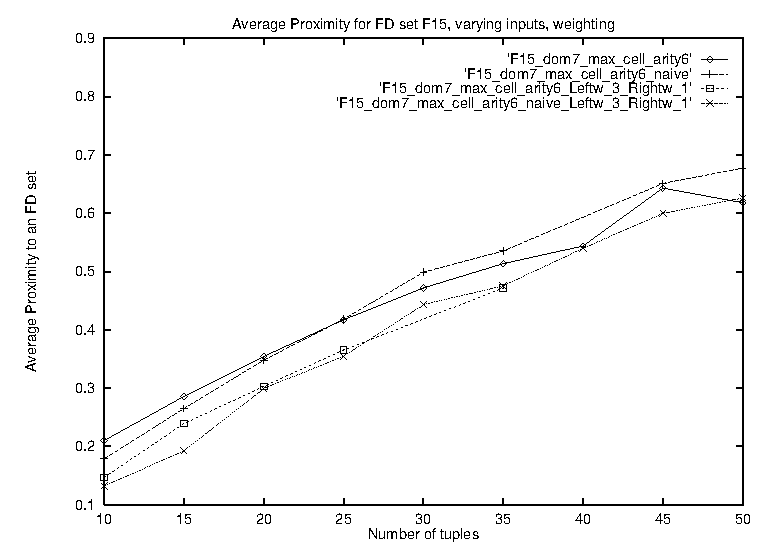
\includegraphics{figures/f15_average.eps}}}
\caption{\label{graph:5.6} {Average Proximity to FD set 15, standard
and reduced
right hand side indefinite cell weighting}}
\end{minipage}
\hfill
\begin{minipage}{7cm}
\centerline{\scalebox{0.5}{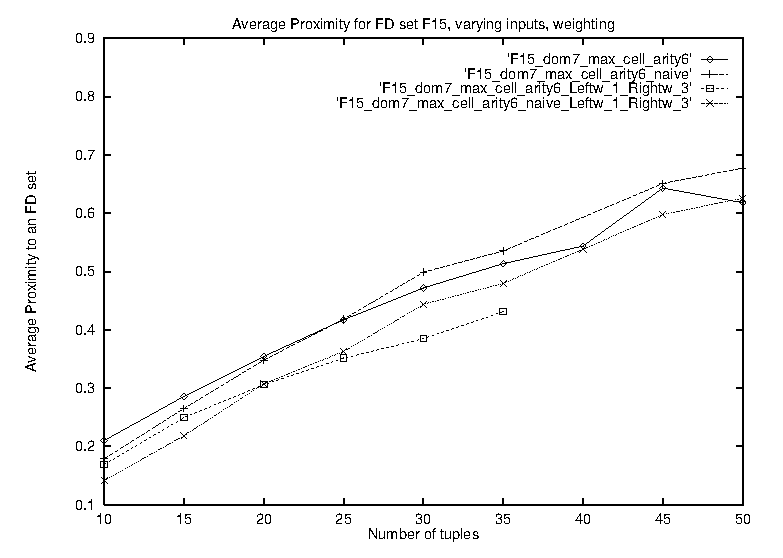
\includegraphics{figures/f15_average2.eps}}}
\caption{\label{graph:5.7} {Average Proximity to FD set 15, standard
and reduced
left hand side indefinite cell weighting}}
\end{minipage}
\end{figure}



\section{Closest Proximity to FD sets}

In contrast with the average results we find that, generally, the
best result within a batch is obtained by our chase and hill-climbing
procedure. Figures~\ref{graph:5.4} and~\ref{graph:5.5}, as well
as~\ref{graph:6.1} and~\ref{graph:5.15}, serve to emphasise that
occasionally the naive procedure, at a cost of efficiency, can
outperform the chase and hill-climbing procedure.


\begin{figure}
\begin{minipage}{7cm}
\centerline{\scalebox{0.5}{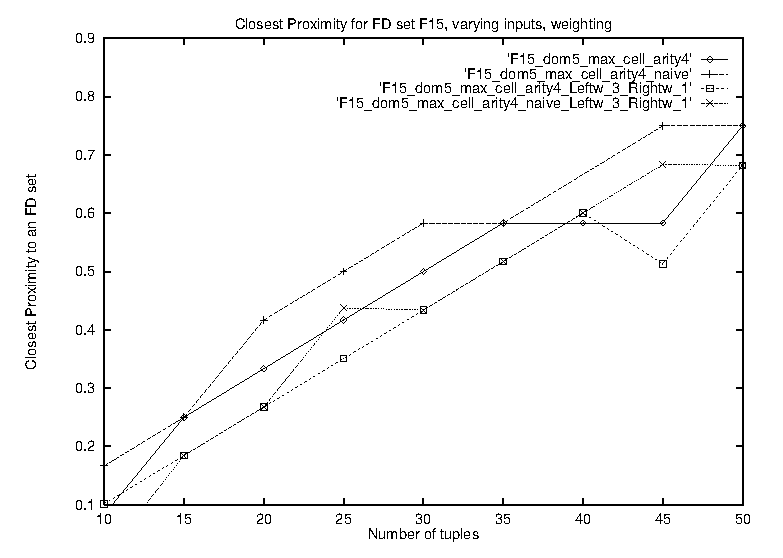
\includegraphics{figures/closest.eps}}}
\caption{\label{graph:5.4} {Closest Proximity to FD set 15 for
standard and reduced right hand side weighting of indefinite cells}}
\end{minipage}
\hfill
\begin{minipage}{7cm}
\centerline{\scalebox{0.5}{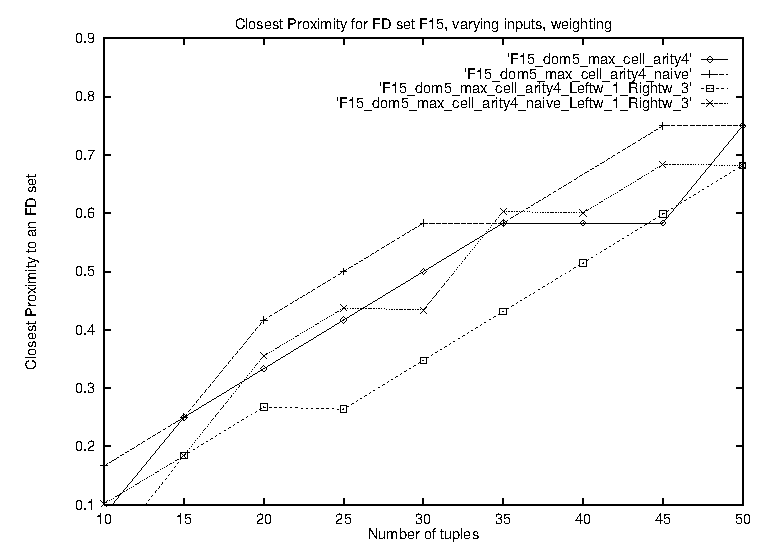
\includegraphics{figures/closest2.eps}}}
\caption{\label{graph:5.5} {Closest Proximity to FD set 15 for
standard and reduced left hand side weighting of indefinite cells }}
\end{minipage}
\end{figure}

\begin{figure}
\begin{minipage}{7cm}
\centerline{\scalebox{0.5}{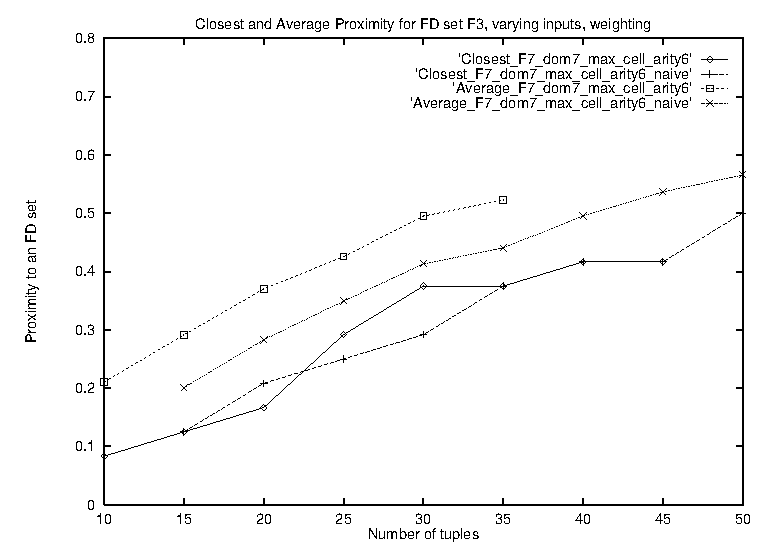
\includegraphics{figures/max2.eps}}}
\caption{\label{graph:5.13} {Average Proximity to  FD set 7, domain
size 7, max indefinite cell arity 6}}
\end{minipage}
\hfill
\begin{minipage}{7cm}
\centerline{\scalebox{0.5}{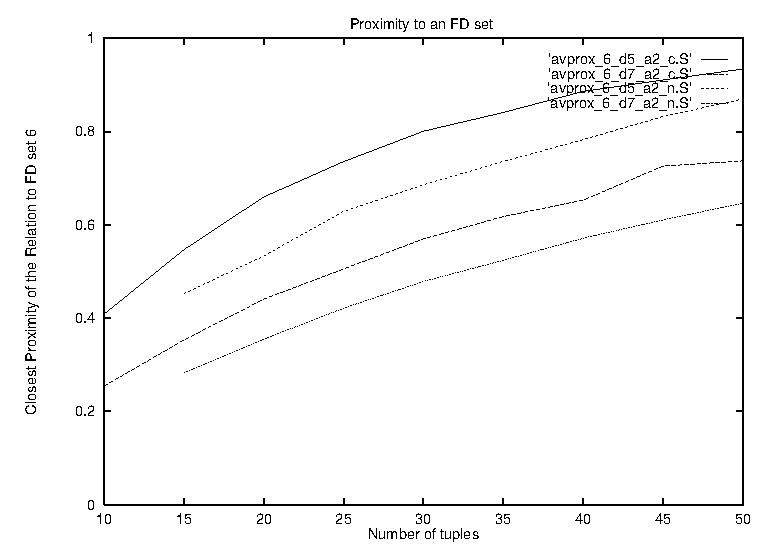
\includegraphics{figures/av6_d5_a2.eps}}}
\caption{\label{graph:5.14} {Average Proximity to FD set 6, domain
5,7, indefinite arity 2}}
\end{minipage}
\end{figure}
\newpage

\begin{figure}
\begin{minipage}{7cm}
\centerline{\scalebox{0.5}{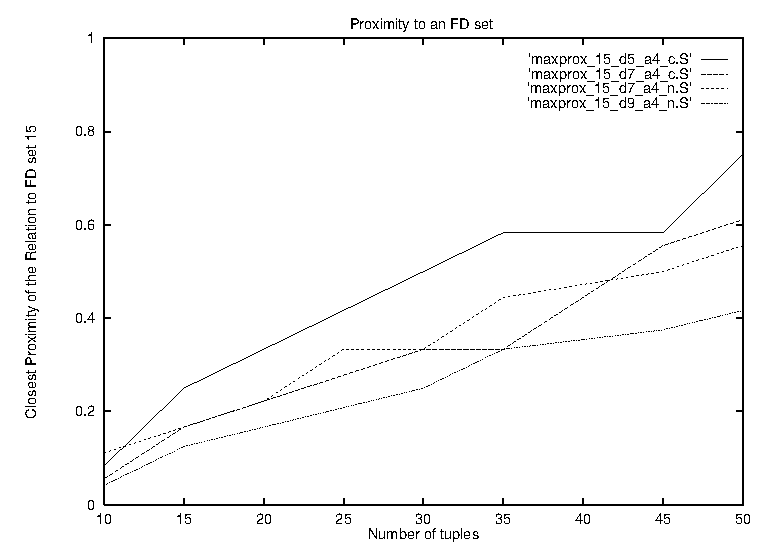
\includegraphics{figures/m15_d5_a4.eps}}}
\caption{\label{graph:6.1} {Closest Proximity to FD set 15, varying
domain sizes 5 - 9, chase and naive approaches, indefinite arity 4}}
\end{minipage}
\hfill
\begin{minipage}{7cm}
\centerline{\scalebox{0.5}{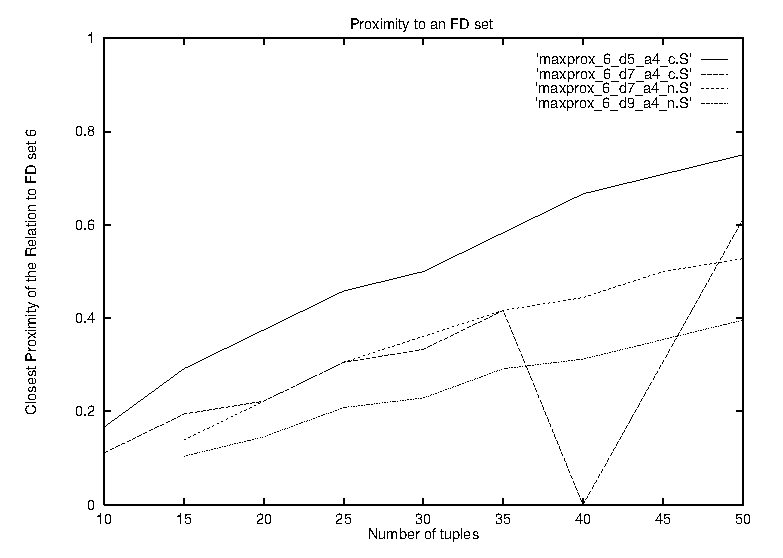
\includegraphics{figures/max6_d5_a2.eps}}}
\caption{\label{graph:5.15} {Closest Proximity to FD set 6, domain
size 5 - 9, indefinite arity 4}}
\end{minipage}
\end{figure}


\section{Jacknife and Bootstrap Comparisons}

Figures~\ref{graph:7.1}, ~\ref{graph:7.2} and~\ref{graph:7.3} present
examples of jackknife and bootstrap resampling used within our dynamic
algorithm~\ref{alg:blimit}. To ensure a fair comparison we conducted
these tests so that at each iteration each sample of possible worlds,
and therefore each sample of ND sets satisfied, was equivalent before
either bootstrap or jackknife resampling was performed. This accounts
for much of the similarity in each figure.

We draw the following conclusions:
\begin{itemize}
\item Jackknife and Bootstrap resampling will reach approximate
fixpoints, on average, at a similar number of possible
worlds. Figures~\ref{graph:7.1}, ~\ref{graph:7.2} and~\ref{graph:7.3}
are indicative of this. 
\item The jackknife resampling technique is more computationally
intensive in such a dynamic setting. The size of the bootstrap
replication is fixed, say at 50 or 100, found to be useful in this
context. \cite{et86,et93} note that sizes about 200 produce no
additional information, in general. However, the jackknife procedure
creates $n$ replicates, each of size $n-1$, when the sample size is
$n$. Therefore we have to examine 299 jackknife resamples at sample
size 300 as opposed to 100 for the bootstrap. The results show this to
be sufficient to infer a suitable standard deviation, variance, or
mean.
\item Jackknife resamples are slightly smoother due to the fact that
we are merely omitting one point in each resample. Though this may
imply it is likely to reach a fixpoint at an earlier stage, results do
not suggest this, validating, in some sense, our approach.
\end{itemize}


\begin{figure}
\begin{minipage}{7cm}
\centerline{\scalebox{0.5}{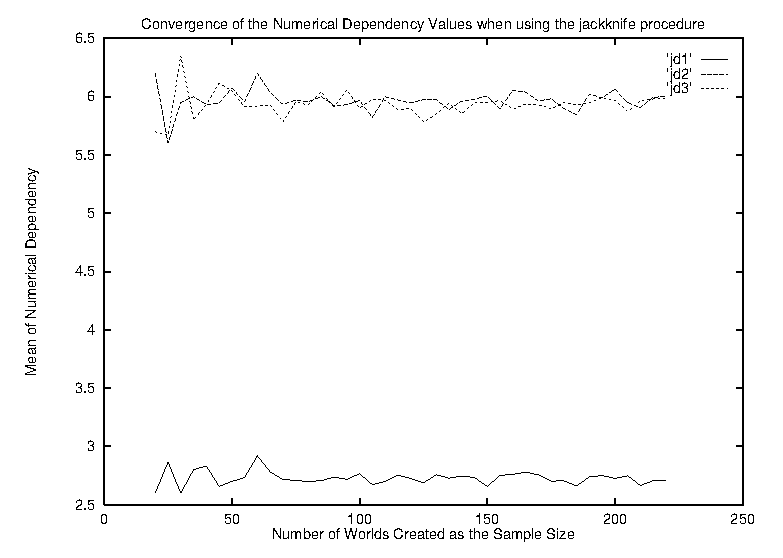
\includegraphics{figures/jack_fd11_10_50_3.eps}}}
\end{minipage}
\hfill
\begin{minipage}{7cm}
\centerline{\scalebox{0.5}{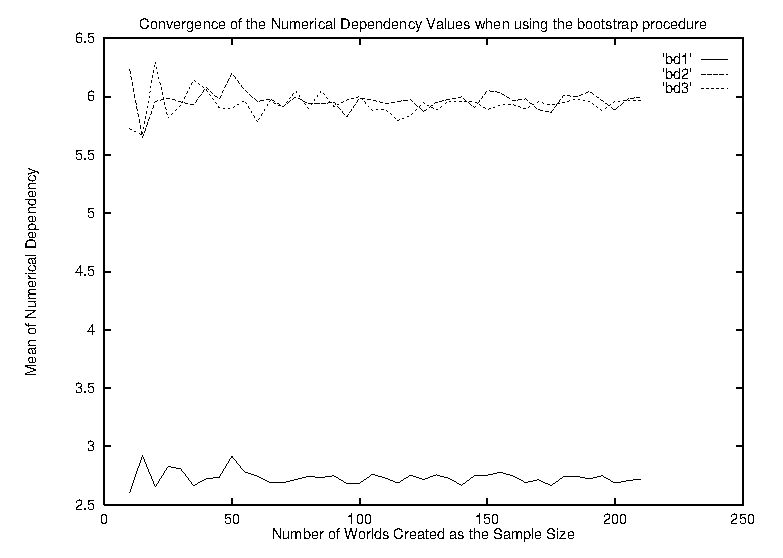
\includegraphics{figures/boot_fd11_10_50_3.eps}}}
\end{minipage}
\caption{\label{graph:7.1} {A comparison of Jackknife and
Bootstrap mean ND set values iterated to an approximate fixpoint of
the mean using equivalent samples, for FD set 11, with a domain of 10,
50 tuples and a maximum indefinite cell arity of 3}}
\end{figure}


\begin{figure}
\begin{minipage}{7cm}
\centerline{\scalebox{0.5}{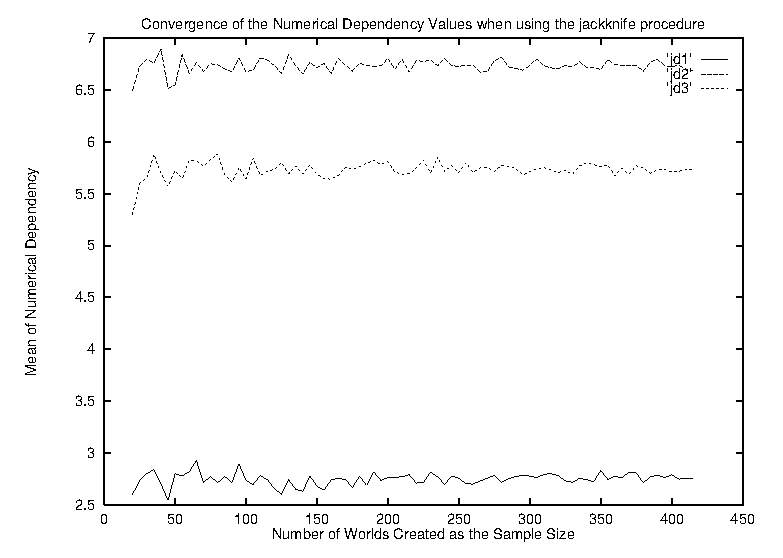
\includegraphics{figures/jack_fd11_10_50_5.eps}}}
\end{minipage}
\hfill
\begin{minipage}{7cm}
\centerline{\scalebox{0.5}{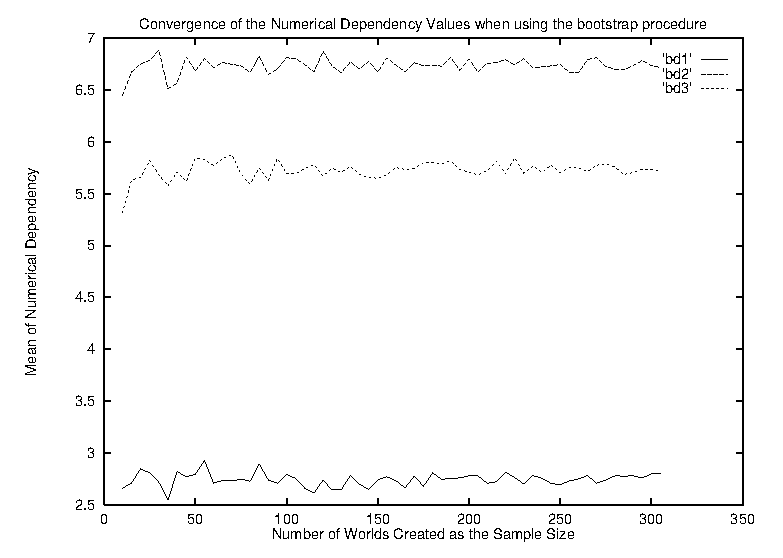
\includegraphics{figures/boot_fd11_10_50_5.eps}}}
\end{minipage}
\caption{\label{graph:7.2} {A comparison of Jackknife and
Bootstrap mean ND set values iterated to an approximate fixpoint of
the mean using equivalent samples, for FD set 11, with a domain of 10,
50 tuples and a maximum indefinite cell arity of 5}}
\end{figure}


\begin{figure}
\begin{minipage}{7cm}
\centerline{\scalebox{0.5}{\includegraphics{figures/jack_fd11_10_25_3.eps}}}
\end{minipage}
\hfill
\begin{minipage}{7cm}
\centerline{\scalebox{0.5}{\includegraphics{figures/boot_fd11_10_25_3.eps}}}
\end{minipage}
\caption{\label{graph:7.3} {A comparison of Jackknife and
Bootstrap mean ND set values iterated to an approximate fixpoint of
the mean using equivalent samples, for FD set 11, with a domain of 10,
25 tuples and a maximum indefinite cell arity of 3}}
\end{figure}


\begin{figure}
\begin{minipage}{7cm}
\centerline{\scalebox{0.5}{\includegraphics{figures/boot_var_fd11_10_50_5.eps}}}
\end{minipage}
\hfill
\begin{minipage}{7cm}
\centerline{\scalebox{0.5}{\includegraphics{figures/boot_sd_fd11_10_50_5.eps}}}
\end{minipage}
\caption{\label{graph:7.4} {Bootstrap variance and standard deviation
convergence, for FD set 11, with a domain of 10, 25 tuples and a maximum indefinite cell arity of 3}}
\end{figure}


Figure~\ref{graph:7.4} highlights convergence of the standard
deviation and variance as the sample size is increased. We are dealing
with approximate fixpoint and this implies equality within confidence
limits shown in Figure~\ref{graph:conlim}. 

\subsection{Bootstrap Variance Results}

\begin{figure}
\begin{minipage}{7cm}
\centerline{\scalebox{0.5}{\includegraphics{figures/var2500.eps}}}
\end{minipage}
\hfill
\begin{minipage}{7cm}
\centerline{\scalebox{0.5}{\includegraphics{figures/var210000.eps}}}
\end{minipage}
\caption{\label{graph:histo2} {Histograms displaying variance of 500 and 10000 bootstrap replications}}
\end{figure}

Figure~\ref{graph:histo2} display the overall similarity in variances
achieved for 500 and 10000 BRS, respectively, complementing
Figure~\ref{graph:cp_hist1}.



\chapter{Simulation Methodology}\label{app:sim_meth}

We now describe our process for conducting experiments, expanding the
outlines given in Chapters~\ref{chap:numdep},~\ref{chap:consistency},
and~\ref{chap:tempresult}, demarcated into sections on evolving
relations, the consistency problem, and simulations on our temporal
logic, respectively.


\medskip
The code was implemented in GNU C++ version 2.7.2 on a UNIX platform running
Sun Solaris 2.5.1.  C++ with
the embedded CORAL deductive
database interface \cite{rss92} was also used for evolving relations
in Chapter~\ref{chap:numdep}. For efficiency reasons the code for procedures
described in Chapters~\ref{chap:consistency} and~\ref{chap:tempresult}
was implemented in C++ alone.
 
\section{Simulation Details: Evolving
Relations}\label{sec:sim_er}

\subsection{Simulation Range Decisions}


We selected 72 FD sets many of which originated from a number of well
known DB texts including \cite{Mann92,databasefound,atze93}. These sets were 
divided into BCNF and non-BCNF for investigative purposes. Given
that an Armstrong Relation can only be generated for a set of FDs F when
the relation size has at least \linebreak $\mid$ GEN(F) $\mid$ + 1
tuples, where 
GEN(F) is defined in Definition~\ref{def:GEN}, then we chose to vary
the domain and tuple sizes from $G/2$ to $G$ and  $G/2$ to $3G$,
respectively. This allowed for the scale of the randomly generated
relations to be related to F, as well as ensuring that we would have a
good chance of finding an AR for each FD set. This choice was
justified by finding ARs in 63 out of our 72 selected FD sets.  We
created a batch of 1000 runs, the process of evolving a randomly
generated relation to absorption, for each domain and tuple
combination. 1000 runs allowed us to find reliable averages for each
domain and tuple combination. 

\medskip

Random Relations were created by random number
selection within a uniform distribution to prevent unwanted
discrepancies in ND set satisfaction. For smaller domain sizes a
normal distribution in random relations would often lead to relations
satisfying FD sets with few steps to absorption as there are likely to
be fewer partitions on attributes on the left hand side of the FDs and
fewer differences between attributes values on the right hand side of the FDs.


\subsection{Use of Random Number Generation}\label{subsec:imp_note}

A number of algorithms in this thesis use randomised techniques. To
circumvent any potential problems with non-random behaviour we used
a linear congruent procedure taken
from the algorithm provided by Park and Miller \cite{pm88} which
avoids cycles by incorporating multiplier and modulus
having 534 million full period generators. 
 
\subsection{C++ libraries}

The program, a direct implementation of Algorithm~\ref{alg:iter},
 was written in C++ with the embedded CORAL deductive
database C++ interface to manipulate the relations. Each randomly
generated relation was created and stored as a database in CORAL.
\smallskip

Via the C++ interface in CORAL, using functional and numerical dependency
classes and a partition class for the tuples, the relation 
 is then mutated according
to the uniform random selections made in the algorithm. C++ with
embedded CORAL was also used for assessing the quality of
the relations after evolution, the knowledge discovery component
of our system.

\section{Simulation Details: The Consistency
Problem}\label{sec:sim_conprob}

For this work we concentrated on 12 FD sets, detailed in
Appendix~\ref{app:con_prob} and Chapter~\ref{chap:consistency}. Again,
for
coverage these were demarcated in BCNF and non-BCNF sets. Our
simulation details are presented in Table~\ref{table:simpar}. The 12
FD sets range from containing a small to a significant number of
dependencies, 8 of which are presented in
Table~\ref{tbl:fd_set_used}. Those FDs not discussed directly within
the text provided results subsumed by those FD sets which are
presented. 

\medskip
For each domain, tuple and maximum indefinite-cell arity we ran a
batch containing 500 runs. A batch was run for both naive and the
chase and hill-climbing instances of the program. Again these batches
allowed us to infer acceptable mean behavior for each input
combination.

\medskip

\subsection{Indefinite Information Data}\label{subsec:ind_inf}

The lack of availability of real-world data containing indefinate
information dictated our use of randomly generated data. Though there
are cases, as we have seen in Chapter~\ref{chap:consistency}, where it
would be useful to represent disjunction within cells, current
RDBMS systems do not generally support anything more than the ability
to store NULL values. This also applies to deductive databases, as
experienced by our use of the CORAL deductive database. Due to this 
we chose to conduct our experiments on randomly generated relations
with a uniform distribution of values across a given domain size.

Further simulations were conducted where attributes on the left hand
side or right hand side of FDs were specified as containing indefinite
cells with either a low, medium, or high probability of containing
indefinite information, as detailed in
Table~\ref{table:spar_range}. This allowed us to study the behaviour
of indefinite information in sparsely generated random relations,
sparsity being elaborated upon in Definition~\ref{def:spar}. 
This direct control over the presence of indefinacy within a randomly
generated relation created with a uniformly random distribution was
preferable to that of a random relation created with a normal
distribution, giving us direct control over the relationship between
indefinacy in cells and their appearance in either the left or right
hand side of an FD.

{\line
\begin{table}[ht]
\begin{center}
\begin{tabular}{|l|l|} \hline 
\multicolumn{2}{|c|} {\bf Sparsity} \\ \hline
{\sc low} & 25\% probability of indefinite cell \\ 
{\sc medium} & 50\% probability of indefinite cell  \\ 
{\sc high}  & 75\% probability of indefinite cell \\ \hline
\end{tabular}
\end{center}
\caption{\label{table:spar_range} Depicting the range of indefinite cells in a relation}
\end{table}
}

\begin{definition}[Sparsity]\label{def:spar}
\begin{rm}
Sparsity is defined to be the fraction of indefinite cells within a 
relation. If relation $R$ has $m$ tuples and $n$ attributes such that it
is of size $m$ x $n$ and there are $k$ indefinite cells in the relation then
its sparsity is $\frac{k}{mn}$. For example a relation with 20 tuples
and 5 attributes will have a low, medium, or high sparsity with 
25, 50, and 75 indefinite cells respectively. $\quad\Box$
\end{rm}
\end{definition}

 

\subsection{A note on randomly generated relations}

The use of randomly generated relations places a limit on the size of
the relations which we can use. For example, as shown in
Table~\ref{table:simpar}, we restricted relation size to 50
tuples. Though this is small given the requirement of a fixed domain
size any increase in relation size is likely to lead to all randomly
created relations satisfying the given FDs as NDs with the branching
factor equivalent to the domain size in all possible worlds. 

\medskip

We stress that though these relations are small there is generally a
significant number of possible worlds to select from.  In a randomly
generated relation with each cell having a 50\% chance of being
indefinite, far higher than likely in the real world, a relation with
50 tuples, 4 attributes and a maximum indefinite cell size of 4 has a
maximum $4^{50.4}$ possible worlds.  A much larger relation, say with
1,000 or 10,000 tuples but with only 20 indefinite cells, none with more
than 4 items in any indefinite cell, would have $4^{20}$ possible
worlds. Larger relations in such a case would not have been any more
comprehensive with regard to results concerning our use of the
bootstrap. 

\subsection{Bootstrap Parameter Size Selection}

The Bootstrap Replication Size (BRS), $B$, is the number of times we
resample from a sample. As discussed in Section~\ref{subsec:boot_proc}
we restate, from \cite{et86}, that there is {\em little improvement}
setting $B$ above 100. We decided to conduct a number of tests with
$B$ starting at 25 and approximately increasing $B$ by a factor of 2
until we reached $B$ = 10,000 on relations. Our tests on a suitable BRS
were conducted on two relations presented together in
Table~\ref{table:brs_testset} with Attribute A as the only left hand
side for the FDs guaranteeing FD violation. These relations contain
every cell as 
indefinite implying that the variance within each resample would be
much higher than for usual implying that our conclusions on a suitable
BRS would be robust for a randomly generated relation. Empirical
results allowed us to conclude that setting $B$ = 100 would provide
reliable resampling results. Figure~\ref{graph:histo2} emphasises the
minimal difference in variance between 500 and 10000 resamples; a
similar result was also found for 100 resamples.


{\line
\begin{table}[ht]
\begin{center}
\begin{tabular}{|c|c|c|c|c|c|} \hline 
 {A } & {\bf B$_1$ } & { \bf B$_2$  } & {\bf $\ldots$ } & {\bf B$_{n-1}$} & { \bf B$_n$ } \\ \hline
$[2,3]$	& $[1,2,3]$ & $[1,2,3]$  & $\ldots$ &  $[1,2,3]$ & $[1,2,3]$ \\
$[2,3]$	& $[4,5,3]$ & $[4,5,3]$  & $\ldots$ &  $[4,5,3]$ & $[4,5,3]$ \\
$\vdots$	& $\vdots$ & $\vdots$  & $\vdots$ &   $\vdots$ & $\vdots$ \\
$[2,3]$	& $[n_{m-3},n_{m-2},3]$ & $[n_{m-3},n_{m-2},3]$  & $\ldots$ &  $[n_{m-3},n_{m-2},3]$ & $[n_{m-3},n_{m-2},3]$ \\
$[2,3]$		& $[n_{m-1},n_m,3]$ & $[n_{m-1},n_m,3]$  & $\ldots$ &  $[n_{m-1},n_m,3]$ & $[n_{m-1},n_m,3]$ \\ \hline
\end{tabular}
\end{center}
\caption{\label{table:brs_testset} Indefinite relations $r_1$ with 10 tuples when $m = 21$ and $r_2$ with
20 tuples and $m = 41$}
\end{table}
}


\subsection{Use of the Original Sample and Fixpoint Selection}

We experimented with 
using the original indefinite 
relation for each resampling iteration from which $n$ possible worlds are
sampled each time. The variance is much higher in this case as we
have all possible worlds to select from for each sample of size
$n$. These experiments were conducted on 5 batches for different
domain, tuple and indefinite cell-arity combinations.

\medskip

Initially we experimented with using our dynamic resampling algorithm,
WORLD\_LIMIT, with different degrees of approximate equality for out
statistical estimators (standard deviation, variance). We found that 1
decimal place to provide too many {\em false} convergence results,
though the averages within a batch were similar to those for 2 decimal
places. We chose to use 2 decimal places as our degree of
approximation in these tests.


\subsection{Using the Bootstrap to determine confidence intervals}

Based on the values generated by the Bootstrap samples we 
used the generally accepted assumption that as the Bootstrap
replication size increases the 
sampling approximates a normal distribution and so we can actually
determine the confidence intervals empirically, shown to converge for
a relation in Figure~\ref{graph:conlim}. For example to find the
95\% confidence intervals we determine what the values of the 
parameter of interest are within the ordered $B$ Bootstrap samples at the
25th and 975th points for the replications with $B$ = 1000. The extra
information provided by confidence intervals for a sample implies that
they need more computational effort, as remarked in \cite{et93}. 

The bootstrap could also be used to find the distribution of {\em good}
approximations to the FD set.
An example of this may be that
NDs such as $AB \to^3 CD$ are found in the $\bar{s}(\tilde{p}^\star_b) + 2.\hat{se}_B$ to
$\bar{s}(\tilde{p}^\star_b) + 3.\hat{se}_B$ 
 range of the distribution  which contains 2.1\% of a normal
distribution, and are therefore considered {\em good} for the
indefinite relation in question.
In this case it will be unlikely to achieve anything better other
than by an exhaustive search which is impossible. Possible problems 
associated with this are that it is too naive to tell us anything
when there may be very few {\em good} approximations such as in
$r_2$, shown in Table~\ref{table:brs_testset}. We chose not to apply this technique.

\medskip

Alternatively we can use the standard error for the Bootstrapped
sample to assign approximate confidence intervals given the
bootstrapped estimate of standard error $\hat{se}_B$ and the bootstrapped variance $\hat{\theta}$ 
whilst assuming a normal distribution.  For example, we determine a 95\% 
confidence interval as $\hat{\theta} \pm 1.960 \cdot \hat{se}_B$.

\subsection{Jackknife and Bootstrap Resampling}

For 3 FDs an additional batch of simulations were run, using
jackknife resampling in addition to bootstrap resampling for 10
different domain/tuple/indefinite-cell arity combinations. We enforced
that each step of resampling would have the same original sample in
each case for more comprehensive comparisons. The only difference was
that for jackknife resampling our statistical estimators would be
based on $n$ resamples for a sample of size $n$ and for 100 resamples
for bootstrapped resamples. This implied that whenever the number of
worlds in a sample exceeded one hundred in our algorithm,
WORLD\_LIMIT, that the bootstrap became more computationally
efficient.

\section{Simulation Details: Numerical Dependency Temporal
Logic}\label{sec:sim_ndltl}

For our simulations on property discovery we used real world data
downloaded from the following sources:

\begin{itemize}
\item Statlib, a data set resource, \ttb http://lib.stat.cmu.edu\tte
\item Financial Data sets are available in the public domain from a
number of sources, we cite \ttb http://www.market-eye.co.uk \tte and
\ttb http://www.moneyworld.co.uk \tte
\end{itemize}

We implemented our objects within template classes in
C++ using the classes for functional and numerical dependencies
created for our work on evolving relations and the consistency
problem. 
A sequence object (class) was created to hold the temporal sequence
data. This was 
implemented as a template in C++ to allow data independence. 
This object contained the required time series function values which
would allow us to difference and create moving averages of the time
series. Additionally it 
included a
sign for the trend, initial and maximum values within the sequence.  
Moving Block procedures were also implemented upon this object.
Statistical functions such as correlations, variance and
covariance were also implemented in this class. 
These time series functions were verified for correctness via
testing and comparison of results presented in \cite{ko90}.
Based on the results of our procedures we are able to add the modal
operators $\bm^n$ and \diam$^n$ to a sequence so that it may represent
a potentially interesting property within our discovery model.


\subsection{Sequence Size Selection}

Input was a Time Series and two sequence sizes.  Given
Theorem~\ref{theorem:pt_logic} we know 
that for fixed small and large sequence sizes the discovery of properties
can be achieved in polynomial time.

We conducted our experiments with a small sequence size $n$ and
large sequence size $2n$. We increased $n$ by a factor of 2 until it
was considered too large to provide meaningful results with respect to
the sequence size at hand, when $n$ is over half the size of the
complete temporal relation sequence implying that all sequences
overlap by at least one point, discussed in
Section~\ref{sec:tr_real_analysis}. 

\medskip


Often we changed the sequence sizes based upon the presence or absence
of response and persistence rules as discussed in
Section~\ref{sec:tr_crit_an}. When the small sequence size $n$ is much
smaller than the large sequence size $m$ then we are unlikely to find
a response rule and if they are nearly the same size we are guaranteed
to find one due to overlapping of sequences. A similar criteria holds
for persistence rules. We found our use of 1:2 as an initial ratio to
provide interesting results, though we freely changed this when
results from simulations suggested so. This highlights the interactive
nature of these simulations, stressed in much data mining research. 


\subsection{Moving Average and Moving Block Size Selection}

Moving Averages ranged from 3 to 10 as our simulation shows. This was
to avoid excessive smoothing with a temporal relation sequence.

\smallskip

Experiments were conducted on a range of different moving block
sizes. These were arbitrary choices based on our goal to obtain
resampled sequences which preserved relationships within the
blocks. The choice of block size in our use of the moving block
bootstrap for large relations depended on our goal of whether we are
seeking to discover properties relating to either grouping of short
ranges or over a {\em synopsis} of the original sequence. Short range
behaviour will be found if we select fewer blocks of a larger size
whilst long range behaviour is found by selecting more blocks of a
smaller size with respect to the size of the original temporal
relation sequence. 










{\setlength{\baselineskip}{13pt}
\printindex
}

\end{document}

